%Document vide aux normes de l'École nationale des Chartes
%crée par J.B. Camps
%Dernières modifications E. Rouquette (03/2025)

%%%%%%%%%%%%%%%%%%%%%% PRÉAMBULE


%%%%%%%%%%%%%% partie obligatoire du préambule
\documentclass[12pt,twoside]{book}
\usepackage{fontspec}
\usepackage{xunicode}
\usepackage[french]{babel} % Utiliser babel pour la gestion des langues
\usepackage{pdfpages}
% \usepackage{polyglossia}
% \setdefaultlanguage[frenchfootnote=true]{french}%indiquer la langue principale du document
% \setotherlanguage{english} %indiquer les autres langues utilisée

%%%%%%%%%%%%%%%%%%%%%%%%%%%%%%%%% PACKAGES UTILISÉS

\usepackage{csquotes}
\setquotestyle{french} % les guillemets français
\usepackage{lettrine} %faire une lettrine (pas obligatoire)
\usepackage[backend=biber,style=biblatex-enc/enc,sorting=nyt,maxbibnames=10, language=french]{biblatex}%charger le style de l'EnC (téléchargeable ici https://ctan.org/pkg/biblatex-enc)
\addbibresource{bibliographie.bib} 

%%%Faire un ou plusieurs index

%\usepackage{imakeidx} %pour faire un ou plusieurs index
%\makeindex %commande pour générer l'index

%RAJOUTEZ ICI VOS PACKAGES

\usepackage{newunicodechar}
\usepackage{graphicx}    % pour includegraphics
\usepackage{subcaption}  % pour les sous-figures
\newunicodechar{•}{\kern-.25em\textperiodcentered\kern-.25em} %Pour le point médian de l'écriture inclusive, faire alt+0183
\newcommand{\wokisme}{\kern-.25em\textperiodcentered\kern-.25em} % Pour l'écriture inclusive comme ça je peux l'appeler avec une commande
\usepackage{listings} % Pour citer du code
\usepackage{graphicx}
\usepackage{float} % Pour fixer les figures et qu'elles ne bougent pas au gré des envies d'Overleaf.

%%%%%%%%%%%%%%%%%%%%%%%%%%%%%%%%% CONFIGURATION DE MISE EN PAGE

%%%%%% Les compteurs (sections, subsections, etc)
\renewcommand{\thechapter}{\arabic{chapter}} % Chapitre en chiffres romains
\renewcommand{\thesection}{\thechapter.\arabic{section}} % Section = Numéro de chapitre + numéro de section
\renewcommand{\thesubsection}{\thesection.\arabic{subsection}} % Subsection = section.sous-section
\renewcommand{\thesubsubsection}{\thesubsection.\arabic{subsubsection}} % Subsubsection = subsection.sous-sous-section
\setcounter{tocdepth}{3} % jusqu'à subsubsection dans la table des matières
\setcounter{secnumdepth}{3} % numérotation affichée jusqu'à subsubsection

%%%%%  Configurer le document selon les normes de l'école
\usepackage{minted} % Pour les blocs de code en couleur
\usepackage{ulem}   % Pour le soulignement
\usepackage[margin=2.5cm]{geometry} %marges
\geometry{margin=2.5cm}
\usepackage{setspace} % espacement qui permet ensuite de définir un interligne
\onehalfspacing % interligne de 1.5
\setlength\parindent{1cm} % indentation des paragraphes à 1 cm

%%%%% Mise en forme des headers (haut de page)

\usepackage{fancyhdr} %package utilisé pour modifier les headers
\pagestyle{fancy} %utiliser ses propres choix de mise en page et non ceux par défaut du package

\setlength\headheight{16pt}%la hauteur des headers

%%la façon dont les sections apparaissent dans les en-tête:

\renewcommand{\sectionmark}[1]{\markright{\small\textit{\thesection~\  #1}}}%Faire apparaître dans les headers les sections en petit et en italiques
%\renewcommand{\sectionmark}[1]{}%Commenter la lign précédetne et mettre celle-ci pour ne pas avoir le titre des sections dans le header

%% réglages propres à frontmatter

\appto\frontmatter{\pagestyle{fancy}%
\renewcommand{\chaptermark}[1]{\markboth{\small\textit{#1}}{}}% ne pas faire apparaître de <<numéro>> de chapitre dans les chapitres non numérotés (front: l'introduction, els remerciement, etc)
}

%% réglages propres à mainmatter

\appto\mainmatter{
\renewcommand{\chaptermark}[1]{\markboth{\small\chaptername~\thechapter~--\ \textit{#1}}{}}}

% Redéfinir les marqueurs pour ne pas inclure les sections
\renewcommand{\sectionmark}[1]{}  % Ne rien faire pour les sections

%% réglages propres aux annexes
\appto\appendix{
  \renewcommand{\chaptername}{Annexe} % Supprime "Chapitre"
  %\renewcommand{\thechapter}{}  % Supprime le numéro
}


%% réglages propres au backmatter
\appto\backmatter{
  \renewcommand{\chaptermark}[1]{}
}

% Redéfinir les marqueurs pour ne pas inclure les sections
\renewcommand{\sectionmark}[1]{}

%%%%%%%%%%%%%%%%%%%%%%%%%%%%%%%%%%%%%%%%%%%%%%%%%%%%%%%%%%%%%%%%%%

%%%%%%%%%%%%%%%%%%%%%%%%%%%%%%%%%%%%%%%%%%%%%%%%%%%%%%%%%%%%%%%%%%

%%%%%%% Package hyperref

% A mettre après les autres appels de packages car redéfinit certaines commandes).

\usepackage[colorlinks=false, breaklinks=true, pdfusetitle, pdfsubject ={Mémoire TNAH}, pdfkeywords={les mots-clés}]{hyperref} %
\usepackage[numbered]{bookmark}%va avec hyperref; marche mieux pour les signets. l'option numbered: les signets dans le pdf sont numérotés

% Compléter pdfsubjet et pdfkeywords
% Explication des options de hyperref (modifiables)
% hyperindex=false
% colorlinks=false: pour que le cadre des liens n'apparaisse pas à l'impression
% breaklinks permet d'avoir des liens allant sur pusieurs lignes
%pdfusetitle: utiliser \author et \title pour produire le nom et le titre du pdf


%avec overleaf, utiliser :
% \usepackage[xetex]{hyperref}
% \hypersetup{
% 		pdfauthor = {Mathieu Taybi},
% 		pdftitle = {Memoire_M2_TNAH_2025},
% 		pdfsubject = {L'IA au Musée des Arts Décos},
% 		pdfkeywords = {\textit{computer vision}} {\textit{machine learning}} {indexation des œuvres}
% 	}


%%%%%%%%%%%%%%%%%%%% Package glossaries

%Exception: il faut le charger APRÈS hyperref
\usepackage[toc=true]{glossaries}
\makeglossaries

%%%%%%%%%%%%%%%%%% DÉFINITION DES COMMANDES ET ENVIRONNMENTS

 %%%%%%%%%%%%%% INFORMATIONS POUR LA PAGE DE TITRE
 
\author{Mathieu \textsc{Taybi} - M2 TNAH}
\title{L'IA au musée des Arts Décoratifs}

%%%%%%%%%%%%%%%%%%%%%% DOCUMENT
\begin{document}
	\begin{titlepage}
		\begin{center}
			
			\bigskip
			
			\begin{large}				
				ÉCOLE NATIONALE DES CHARTES\\
				UNIVERSITÉ PARIS, SCIENCES \& LETTRES
			\end{large}
			\begin{center}\rule{2cm}{0.02cm}\end{center}
			
			\bigskip
			\bigskip
			\bigskip
			\begin{Large}
				\textbf{Mathieu Taybi}\\
			\end{Large}
		%selon le cas
			\begin{normalsize} \textit{licencié ès de philosophie}\\
				\textit{diplômé de master de philosophie et d'histoire}
			\end{normalsize}
			
			\bigskip
			\bigskip
			\bigskip
			
			\begin{Huge}
				\textbf{L'IA au Musée des Arts décoratifs}\\
			\end{Huge}
			\bigskip
			\bigskip
			\begin{LARGE}
				\textbf{Perspectives et opportunités pour le traitement massif des collections patrimoniales}\\
			\end{LARGE}
			
			\bigskip
			\bigskip
			\bigskip
			\begin{large}
			\end{large}
			\vfill
			
			\begin{large}
				Mémoire 
				pour le diplôme de master \\
				« Technologies numériques appliquées à l'histoire » \\
				\bigskip
				2025
			\end{large}
			
		\end{center}
	\end{titlepage}
	
\frontmatter

%%%%%%%%%%%%%%%%%%%% RESUMÉ %%%%%%%%%%%%%%%%%%%%%%%%%%

	\chapter{Résumé}
\medskip
	Ce mémoire a été réalisé à la suite d'un stage de 6 mois au sein du Département des Arts graphiques du musée des Arts décoratifs de Paris. L'objectif principal de ce stage était d'explorer et de mettre en place plusieurs outils technologiques de reconnaissance d'images dans le cadre du traitement des collections du musée. Nous avons poursuivi cet objectif en empruntant deux voies distinctes et complémentaires. La première était centrée sur un projet d'apprentissage supervisé avec un modèle de \textit{computer vision} sur le fonds de dessins du designer Jean Royère, afin d'automatiser la reconnaissance des motifs et des meubles sur les calques et les gouaches qu'il a produit. La seconde se concentrait sur le recueil des besoins, la formation et l'acculturation des équipes scientifiques aux nouveaux outils et procédés utilisant l'intelligence artificielle. Nous avons cherché à retranscrire en termes technologiques les demandes pratiques des équipes du musée qui ont pour mission la gestion et la conservation des collections d'arts graphiques. 
    
    Ce mémoire s'attache donc à décrire les différentes approches et technologies déployées pour appliquer un traitement de \textit{computer vision} à des collections patrimoniales uniques dans un musée tout aussi unique. Nous présentons un regard rétrospectif sur le musée, un état des lieux de sa situation, un compte-rendu des résultats obtenus par les technologies déployées ainsi que différentes stratégies et perspectives pour l'intégration durable des nouveaux outils d'intelligence artificielle dans le cadre du traitement des collections. \\
	
	\textbf{Mots-clés:} TNAH ; \textit{Computer vision} ; \textit{Machine learning} ; Intelligence artificielle ; YOLO ; Indexation des œuvres ; Histoire du musée.
    
%%%%%%%%%%%%%%%%%%%% MOT-CLEFS & CITATION %%%%%%%%%%%%%%%%

	\textbf{Informations bibliographiques:} Mathieu Taybi, \textit{L'IA au musée des Arts décoratifs. Perspectives et opportunités pour le traitement massif des collections patrimoniales}, mémoire de master « Technologies numériques appliquées à l'histoire », dir. Marion Charpier, École nationale des chartes, 2025.

%%%%%%%%%%%%%%%%%%%% REMERCIEMENTS %%%%%%%%%%%%%%%%%%%%%%

	\chapter{Remerciements}
    
Je tiens à remercier tout d'abord Sonia Aubès pour m'avoir accueilli au sein du Département des Arts graphique du musée des Arts décoratifs de Paris, et pour sa relecture du présent travail. Je remercie également toute l'équipe du département pour leur accueil exceptionnel et leur gentillesse. Je remercie spécifiquement Sébastien Quéquet du département pour son enthousiasme dans le projet et pour sa participation au jury de soutenance.

Je remercie chaleureusement Marion Charpier pour sa supervision, sa bonne humeur et ses précieux conseils tout au long de ce stage unique et stimulant. Je remercie aussi Emmanuelle Bermès pour son encadrement, sa direction et pour m'avoir fait confiance sur ce projet. Je remercie Nathan Schlanger d'avoir accepté de présider le jury de soutenance.

Je remercie tout particulièrement Léa pour sa relecture patiente et bienveillante, et pour ses précieux conseils qui m'ont permis de clarifier mon propos et de reformuler certains passages obscurs. 

Je remercie aussi tous\wokisme tes les ami\wokisme e\wokisme s, de Paris et d'ailleurs, qui m'ont permis d'aborder cette aventure nouvelle dans le monde de l'informatique appliquée aux sciences humaines, et de partager mes peines et mes joies pendant cette année dense et rude à plusieurs égards. 

Sans oublier de remercier particulièrement Francesca pour sa présence à mes côtés, sa vivacité d'esprit et sa relecture attentionnée.

Enfin, je tiens à remercier Shiva, petite boule de poils qui me suit depuis 10 ans déjà, de m'avoir accompagné et apporté son soutien muet et indéfectible, surtout pendant la dernière phase de ce travail de rédaction .

%%%%%%%%%%%%%%%%%%%%%%%%%%%%%%%%%%%%%%%%%%%%%%%%%%%%%%%%%
%%%%%%%%%%%%%%%%%%%% BIBLIOGRAPHIE %%%%%%%%%%%%%%%%%%%%%%
%%%%%%%%%%%%%%%%%%%%%%%%%%%%%%%%%%%%%%%%%%%%%%%%%%%%%%%%%
        
\nocite{*}
\chapter{Bibliographie}
\section*{}
\defbibheading{firstlevel}{\section*{#1}}
\defbibheading{secondlevel}{\subsection*{#1}}

\printbibliography[keyword=Archives, title=Archives, heading=firstlevel]
\clearpage
\printbibliography[keyword=Articles, title=Articles, heading=firstlevel]
\printbibliography[keyword=Po, title=Discours politiques et interviews, heading=firstlevel]
\printbibliography[keyword=Législation, title=Législation, heading=firstlevel]
\printbibliography[keyword=Monographies, title=Monographies, heading=firstlevel]
\printbibliography[keyword=Th, title=Thèses et mémoires, heading=secondlevel]
\printbibliography[keyword=Sites web, title=Sites web, heading=firstlevel]
\printbibliography[keyword=Vid, title=Vidéos, heading=firstlevel]

%%%%%%%%%%%%%%%%%%%%%%%%%%%%%%%%%%%%%%%%%%%%%%%%%%%%%%%%%%
%%%%%%%%%%%%%%%%%%%% CORPS DU MEMOIRE %%%%%%%%%%%%%%%%%%%%
%%%%%%%%%%%%%%%%%%%%%%%%%%%%%%%%%%%%%%%%%%%%%%%%%%%%%%%%%%

%%%%%%%%%%%%%% INTRO %%%%%%%%%%%%%%%%%%%%%%%%%%%%%%%%%%%%%
%%%%%%%%%%%%%%%%%%%%%%%%%%%%%%%%%%%%%%%%%%%%%%%%%%%%%%%%%%
	
\chapter{Introduction}

Le présent travail intervient à la fin de la première année de lancement du projet TORNE-H au musée des Arts décoratifs. L'acronyme du projet signifie \enquote{Traitement d'objets par reconnaissance numérique en environnement humain}. Il est aussi l'anagramme d'Henrot, nom du photographe autour duquel s'est agencé l'idée du projet. Il est le fruit d'une collaboration entre trois institutions : la Bibliothèque Nationale de France, par l'entremise de son chef de mission Intelligence Artificielle Jean-Philippe Moreux ; le Centre Jean Mabillon de l'École des Chartes sous la direction d'Emmanuelle Bermès ; et le musée des Arts décoratifs sous les auspices de Camille Herody, directrice générale adjointe du musée. Il a été rendu possible grâce à un financement du Ministère de la Culture dans le cadre du Fonds d’accompagnement à la transformation numérique et à la cybersécurité des établissements du ministère de la Culture (FTNC). 

Le projet se place dans le cadre de la nouvelle stratégie \textit{data} du musée des Arts décoratifs. Il ambitionne de \enquote{mettre au point des flux de traitements des collections muséales avec une utilisation de l'intelligence artificielle pour l'analyse et la description automatique des données visuelles}\footnote{\cite{grim_vision_2024}. p. 8.}. Il est le résultat de deux ans de tests préalables, pilotés par Marion Charpier et Emmanuelle Bermès, sur le fonds du designer Jean Royère (1902-1981), riche de 18 000 dessins et gouaches non décrites. Cette première phase a consisté en une réflexion sur les outils et les méthodes à adopter dans le cadre d'une tâche de description de fonds patrimoniaux. Elle s'est accompagnée d'un travail de compréhension et de recueil des besoins des personnels du musée, afin de cibler au mieux les outils et procédés adaptés et réplicables à d'autres contextes et collections. L'un des enjeux principaux pour le musée est d'être en mesure de décrire ses collections pour venir alimenter la base de données. Les personnels du musée estiment que seulement 30\% des collections sont décrites, et pour le département des Arts graphiques seul, cela représente 700 000 pièces non décrites ou inventoriées. \hfill \break
\hfill \break

Dans ce cadre, les équipes du musée veulent avoir recours à des processus automatisés comme la vision par ordinateur tout en gardant une exigence haute de fiabilité. Le \textit{workflow} qui a été construit pendant ce projet se base sur un dialogue constant avec les équipes scientifiques du musée et sur la nécessaire validation des informations produites par les responsables des collections. Dans le sillage de la refonte de sa stratégie \textit{data}, adoptée en octobre 2023, le musée a fait appel au centre Jean Mabillon pour explorer les techniques avancées d'analyses d'images par IA. \enquote{Il s’agit de démontrer la valeur ajoutée de l’IA pour le traitement des collections et
de tester l’intégration des données générées au sein des processus métiers propres à la gestion
des collections nationales. La data structure et les stratégies d’entraînements adoptées au
terme du projet Royère constitueront un socle technique dans la mise au point de la nouvelle
infrastructure numérique du musée – applicable à l’ensemble de ses collections}\footnote{\cite{grim_vision_2024}. p. 8.}.

Nous revenons ici sur quelques notions fondamentales en traitement automatisé et en intelligence artificielle, afin de poser certains définitions que nous devons manipuler par la suite. Tout d'abord qu'est-ce que l'intelligence artificielle ? Elle est définie par la CNIL comme \enquote{un procédé logique et automatisé reposant généralement sur un algorithme et en mesure de réaliser des tâches bien définies. Pour le Parlement européen, constitue une intelligence artificielle tout outil utilisé par une machine afin de \textquotedblleft reproduire des comportements liés aux humains, tels que le raisonnement, la planification et la créativité \textquotedblright{}}\footnote{\cite{cnil_intelligence_nodate}}. Elle est de deux types : elle peut être connexionniste ou symbolique. Dans le premier cas, elle s'inspire du fonctionnement du cerveau humain et de son réseau de neurones biologiques, elle ne s'appuie pas sur des règles explicites, mais \enquote{apprend} à partir de données pour extraire des motifs et des relations à partir de nouvelles données\footnote{\cite{charpier_atelier_2025}}.Dans le second cas, elle s'appuie sur des règles explicites préprogrammées pour prendre des décisions. Elle ne demande pas de passer par un apprentissage à partir de données mais elle suit des règles préétablies. 

Maintenant, qu'est-ce la vision par ordinateur ou \textit{computer vision} ? \enquote{La vision par ordinateur est une branche de l’intelligence artificielle dont le principal but est de permettre à une machine d’analyser et traiter une ou plusieurs images ou vidéos prises par un système d’acquisition}\footnote{\cite{carius_lexique_2024}}. La vision par ordinateur utilise un modèle d'IA de type connexionniste. Un modèle IA est un algorithme capable (avec plus ou moins d’efficacité) d’effectuer un ensemble de tâches pour lesquelles on l’a entraîné\footnote{\cite{noauthor_quest-ce_2023}}. Il reçoit un type de données en entrée, et en propose un autre en sortie. Le terme “modèle” s’applique en IA peu importe le domaine. On appelle un modèle qui peut recevoir plusieurs types de données en entrée (par exemple texte ET image), un modèle multimodal. On distingue aussi généralement les modèles spécialisés, capables de réaliser une unique tâche (par exemple détecter les visages sur une image), des modèles généralistes capables de réaliser des tâches très variées (comme la plupart des \textit{Large Language Models}). Les modèles spécialisés requièrent habituellement moins de puissance de calcul que les généralistes.

Pour l'entraînement des modèles on distingue deux approches : la première est l'apprentissage machine ou l'apprentissage automatique, c'est-à-dire sans supervision. Il consiste en un \enquote{processus par lequel un algorithme évalue et améliore ses performances sans l’intervention d’un programmeur, en répétant son exécution sur des jeux de données jusqu’à obtenir, de manière régulière, des résultats pertinents. Un algorithme d’apprentissage automatique comporte un modèle dont il modifie les paramètres, de valeur initiale en général aléatoire, en fonction du résultat constaté.}\footnote{\cite{carius_lexique_2024}}. La seconde est l'apprentissage au sein duquel on trouve des interventions humaines explicites comme l'apprentissage supervisé ou l'apprentissage par renforcement\footnote{\textit{cf}. le \textbf{\hyperref[sec:Glossaire]{Glossaire}} pour les termes \enquote{apprentissage supervisé} et \enquote{apprentissage par renforcement}, p.~\pageref{sec:Glossaire}.}.

Afin de comprendre le projet qui a précédé le notre, nous devons parler de la spécificité du fonds Royère. En premier lieu, il est clos, c'est-à-dire qu'il ne recevra plus de nouvelles additions. Il comprend la majeure partie de la production de l'artiste, légué après sa mort. Il se compose de vues, en couleurs ou au fusain, de meubles ou de pièces qu'il a réalisé pour ses clients. De même, on dispose aussi d'un plan de classement réalisé par l'artiste et il y a une grande récurrence des mêmes types d'objets dans les dessins. C'est d'ailleurs ce qui a pu amener à l'établissement d'une ontologie fixe pour le traitement automatisé. Quelle a donc été la nature de ce traitement ?

Les résultats de ce premier projet font apparaître plusieurs éléments déterminantes sur lesquelles le projet TORNE-H a été bâti. Dans la démarche de comparaison des performances des modèles, deux approches ont été explorées : l'une via l'apprentissage supervisé avec \mbox{YOLOv8} et l'autre via un modèle \textit{zero-shot} Clip développé par OpenAI\footnote{\textit{cf}. le \textbf{\hyperref[sec:Glossaire]{Glossaire}} pour le terme \enquote{Clip} , p.~\pageref{sec:Glossaire}.}. Ici il faut entendre \textit{zero-shot} comme un modèle n'étant pas passé par une phase d'entraînement. Clip est un modèle qui a été entraîné sur 1,28 millions d'images issues d'internet et accompagnées de légendes, et il se base sur cette connaissance pour décrire les choses qu'on lui propose. \hfill \break

L'intérêt de ce modèle réside dans sa \enquote{capacité [...] à réaliser une
tâche pour laquelle il n’a pas été spécifiquement entraîné. Cela est possible grâce à l’espace
d’enchâssement vectoriel constitué lors de l’entraînement de CLIP\footnote{\textit{cf}. \enquote{Espace vectoriel} dans le \textbf{\hyperref[sec:Glossaire]{Glossaire}}, p.~\pageref{sec:Glossaire}.}. Les représentations vectorielles
lui permettent de correctement associer des images et des descriptions textuelles jamais
vues pendant son apprentissage}\footnote{\cite{grim_vision_2024}. p. 63.}. Cependant, l'approche qui a été privilégiée, et dont nous avons hérité est celle de l'apprentissage supervisé par l'entraînement d'un modèle YOLO avec une ontologie définie.

Dans les grandes lignes un processus d'entraînement par \textit{fine-tuning} consiste en une boucle de traitement qui a pour but la spécialisation d'un modèle pré-existant, ici YOLOv8, sur une tâche, ici la reconnaissance des meubles du fonds Royère\footnote{\textit{cf}. le \textbf{\hyperref[sec:Glossaire]{Glossaire}} pour le terme \enquote{\textit{fine-tuning}}, p.~\pageref{sec:Glossaire}.}. Ce processus passe par une phase d'annotation manuelle de données afin de constituer une vérité terrain\footnote{\textit{cf}. le \textbf{\hyperref[sec:Glossaire]{Glossaire}} pour les termes \enquote{vérité terrain} et \enquote{annotation manuelle}, p.~\pageref{sec:Glossaire}.}. Cette vérité terrain est le standard, la source fiable d'informations pour l'algorithme, parce que réalisé à la main. Ensuite, on entraîne l'algorithme à partir de cette vérité terrain pour lui apprendre à reconnaître les objets, via un système de poids et de biais en le lançant d'abord sur les mêmes images que la vérité terrain afin de produire des \textit{metrics} pour mesurer ses performances\footnote{\textit{cf}. le \textbf{\hyperref[sec:Glossaire]{Glossaire}} pour le terme \enquote{\textit{metrics}}, p.~\pageref{sec:Glossaire}.}. Puis on le lance sur des images qu'il ne connaît pas et on répète le processus en corrigeant ses prédictions, en ajoutant ces corrections à la vérité terrain et ainsi de suite, jusqu’à obtenir des \textit{metrics} satisfaisantes. Nous reviendrons sur le détail de ce processus et de ces \textit{metrics} dans la partie dédiée au \textit{machine learning} dans le chapitre 5.

Pour notre part, après cette mission technique de développement et de raffinement des solutions proposées nous intervenons au niveau de la réflexion sur la stratégie à adopter pour l'introduction pérenne d'outils d'IA dans le musée. Nous avons été auprès des équipes pour participer à leur acclimatation à ces outils, pour recueillir les avis et attentes des personnels, et pour mettre en œuvre un premier processus de MLOps au sein du musée avec ses infrastructures existantes\footnote{\textit{cf}. le \textbf{\hyperref[sec:Glossaire]{Glossaire}} pour le terme \enquote{MLOps}, p.~\pageref{sec:Glossaire}.}. Ce travail de rédaction est le reflet de cette activité, et il va tenter de répondre à plusieurs questions indispensables pour la mise en place d'un modèle d'intelligence artificielle dans le but de décrire les collections du musée. 

Nous nous interrogeons sur les limites et opportunités qu'offrent les modèles actuels pour la description patrimoniale. Ce faisant nous nous posons la question de la dette technique et du passif d'une institution vis-à-vis de son traitement des collections. Nous interrogeons en outre l'état de l'art dans la recherche en humanités numériques, sur des questions de recherches similaires, afin de voir quels choix ont été faits et quels problèmes ont été rencontrés ailleurs. Enfin, nous tentons de souligner les obstacles et points de vigilances à garder en tête au sujet de l'introduction d'une technologie d'intelligence artificielle dans le cadre de collections publiques et d'institutions patrimoniales.

Afin de répondre à ces questions, nous commençons ce travail par un bref retour rétrospectif sur l'histoire de l'Union Centrale des Arts Décoratifs depuis le milieu du \textsc{xix}\textsuperscript{e}~siècle jusqu'à nos jours. Cette partie nous permet de replacer la spécificité du MAD dans son contexte, d'étudier son évolution organisationnelle, l'émergence de l'idée d'un musée dédié aux arts décoratifs, l'importance de l'initiative privée et le rôle de l'État dans cette institution. Elle permet aussi de donner à voir la manière dont les collections se sont constituées au fil du temps afin de mieux saisir la particularité de celles-ci et les problèmes qu'elles posent aux personnels scientifiques aujourd'hui. 

Dans un second temps, nous traitons de l'environnement de recherche dans lequel se situe le projet en le replaçant au sein des interactions et institutions auquel il appartient. Nous passons en revue un certains nombre d'acteurs, publiques ou privés, qui participent à l'élaboration de ces nouveaux terrains de recherches en sciences humaines, permis par les avancées technologiques récentes. Puis, nous rendons compte de notre mission vis-à-vis de l'entraînement du modèle pour la production des notices d'inventaires du fonds Royère, et nous abordons la production de code et le déploiement logiciel que nous avons mené. Enfin, nous revenons sur le fruit des entretiens menés sur les équipes à propos de leur utilisation de l'IA.

Ainsi, fort de ces connaissances et de cette vue sur le contexte institutionnel et théorique dans lequel s'inscrit l'IA, nous tentons, dans une dernière partie, d'ouvrir la discussion sur les limitations identifiées et les préconisations pour l'introduction durable de la \textit{computer vision} au musée de Arts décoratifs spécifiquement, et plus généralement dans une institution patrimoniale. 

\mainmatter

%%%%%%%%%%%%%% PART 1 %%%%%%%%%%%%%%%%%%%%%%%%%%%%%%%%%%%
%%%%%%%%%%%%%%%%%%%%%%%%%%%%%%%%%%%%%%%%%%%%%%%%%%%%%%%%%

\part{Socio-histoire d'un musée à part}

%%%%%%%%%%%%%%%%%%%%%%%%%%%%%%%%%%%%%%%%%%%%%%%%%%%%%%%%%%%%%%%%%%%%%%%%%%%%%%%%%%%%
%%%%%%%%%%%%%%%%%%%%%%%%%%%%%%%%%%%%%%%%%%%%%%%%%%%%%%%%%%%%%%%%%%%%%%%%%%%%%%%%%%%%
%%%%%%%%%%%%%%%%%%%%%%%%%%%%%%%%%%%%%%CHAPITRE%%%%%%%%%%%%%%%%%%%%%%%%%%%%%%%%%%%%%%
%%%%%%%%%%%%%%%%%%%%%%%%%%%%%%%%%%%%%%%%%%%%%%%%%%%%%%%%%%%%%%%%%%%%%%%%%%%%%%%%%%%%
%%%%%%%%%%%%%%%%%%%%%%%%%%%%%%%%%%%%%%%%%%%%%%%%%%%%%%%%%%%%%%%%%%%%%%%%%%%%%%%%%%%%

\chapter{Une bibliothèque, un musée et une association unique en France, au service du « Beau dans l’Utile »}

\section{Le \textsc{XIX}\textsuperscript{e}~siècle et les arts décoratifs}

Au cours de ce siècle d'intense industrialisation, la position de l'artiste à l'intérieur de la société évolue. La dimension holistique du \enquote{savoir technique de l'artisan est niée et fragmentée par la division du travail, il se transforme en exécuteur passif d'une œuvre dont la conception ne lui appartient plus}\footnote{\cite{froissart_union_1990}. p. 1.}. Le statut de l’œuvre change aussi, elle perd sa connotation artistique originale du fait de sa reproductibilité technique, et se retrouve dépourvue de son \enquote{aura}\footnote{\cite{benjamin_walter_oeuvre_2013}}. À partir des années 1830, et au fil des expositions universelles, les arts industriels s'imposent petit à petit mais ne gagnent jamais la dignité réservée aux Beaux-Arts. On les considère comme des objets \enquote{produit à bon marché et en série, [...] forcément laids}\footnote{\cite{froissart_union_1990}. p. 11.}. Il faut attendre 1861 pour voir en France une première exposition dédiée aux arts industriels. Elle ne voit le jour qu'\enquote{avec des moyens limités et grâce à l'initiative privée}\footnote{\cite{froissart_union_1990}. p. 17.}. 

Les initiateurs de cette exposition sont ceux qui sont aussi derrière la fondation d'une association dédiée aux arts industriels quelques années plus tard. Ils ont pour ambition l’anoblissement de ces arts et leur pleine inscription dans le paysage artistique de leur époque. Cette entreprise de légitimation est la mieux représentée par la position d'un homme de lettres et journaliste, Théodore Labourieu, qui joue un rôle majeur en faveur des arts décoratifs en ce milieu du \textsc{xix}\textsuperscript{e}~siècle. Il \enquote{engage une vraie bataille contre tous ceux qui veulent reléguer les arts appliqués dans le domaine méprisé de l'industrie et du commerce, indignes donc de rechercher le vrai beau \textit{idéal}}\footnote{\cite{froissart_union_1990}. p. 33.}. Il critique le "grand Art" qu'il appelle "abstrait", et à qui il reproche d'appartenir à la sphère de l'idéal et non de la réalité concrète. Il va plus loin en disant qu'\enquote{il n'est pas l'expression de son époque ; [et que] seul l'art qui contribue directement à satisfaire les besoins pratiques de l'homme est capable d'exprimer son siècle , le siècle du \textquotedblleft Travail \textquotedblright{}}\footnote{\cite{labourieu_art_1857}. p. 261.}.
Son ambition est de rapprocher l'art du public, et il voit dans l'art uni au travail, dans le syncrétisme entre artiste et ouvrier, la voie que doit emprunter l'art nouveau dessinée par ce siècle industrieux. C'est animé d'une foi dans le travail comme moyen de progrès, empreinte des idées des socialismes contemporains et du saint-simonisme que Labourieu théorise cette mise à la portée de l'art pour chacun\footnote{\cite{froissart_union_1990}. p. 33.}. 

\subsection{Fondation et historique de l'association}

L'histoire du l'entité qui regroupe deux musées, une école, une bibliothèque et une association sous le même sigle "MAD" de nos jours, remonte à cette deuxième moitié de \textsc{xix}\textsuperscript{e}~siècle et prend racine dans deux mémoires et un placet remis à Charles Louis Napoléon Bonaparte alors président de la Deuxième République, peu de temps avant la proclamation de l'Empire. Ces documents lui sont remis le 25 novembre 1852\footnote{\cite{noauthor_origines_nodate}. p. 3.} à Saint-Cloud de la part du "Comité central des artistes et des artistes industriels" qui représente 126 artistes, dessinateurs industriels, architectes, sculpteurs, graveurs, ornemanistes et joailliers. Le but de ces doléances est \enquote{de demander à l'État d'instaurer un musée des beaux-arts industriels, une école centrale des beaux-arts appliqués à l'industrie et des expositions spéciales des œuvres des artistes industriels}\footnote{\cite{noauthor_origines_nodate}. p. 3.}. 

Ces doléances restent lettre morte, et c'est Théodore Labourieu qui, en 1855, reprend le propos de ces mémoires et décide d'en soutenir les visées par la création de la revue \textit{L'art au \textsc{xix}\textsuperscript{e}~siècle}\footnote{\cite{froissart_union_1990}. p. 21.}. C'est dans cette revue que sont publiés les premiers statuts de l'association du nom de Société pour le Progrès des Arts Industriels en 1858, présidé par M. Mirault, à la suite de la présentation d'un projet d'école et de musée au Conservatoire des Arts et Métiers le 14 juillet 1856\footnote{\cite{froissart_union_1990}. p. 23.}. 
À l'origine le musée ne devait \enquote{qu'être complémentaire à l'école, [...] pour que les ouvriers puissent avoir le temps de visiter ses collections de modèles}\footnote{\cite{froissart_union_1990}. p. 36.}. L'idée principale est la création d'une école d'arts appliqués au sein du Conservatoire des Arts et Métiers, et les initiateurs savent que le musée sera le résultat d'une démarche plus longue.

Après plusieurs années de tentatives d'expositions infructueuses c'est Édouard Guichard qui obtient, avec le concours du baron Taylor, une première exposition fin 1861 au Palais de l'Industrie. 
\vspace{1em}

\noindent
\hspace*{1cm}
\begin{minipage}{\dimexpr\linewidth-2cm}
\fontsize{10}{12}\selectfont
Le but de l'initiative est de pousser les artistes à une émulation féconde, de mieux définir leurs place à l'intérieur de domaines éloignés comme ceux de l'industrie et de l'art [et peut-être d'amener] l'art industriel à une fonction vulgarisatrice de l'idée du \textit{beau}, \textit{vrai}, et \textit{bien}                                                        \footnotemark{}
\end{minipage}

\vspace{1em}

\footnotetext{insère la ref bibliographique}

\footnotetext{\cite{froissart_union_1990} p. 40.}

Après l'exposition de 1863, la Société pour le Progrès des Arts Industriels entre en crise profonde et se dissout, ce qui amène la fondation en 1864 de l'Union centrale des Beaux-Arts appliqués à l'Industrie dont le siège est établi au 3 places des Vosges, au plus près des ouvriers du Marais. Dans ses statuts, son but est \enquote{d'entretenir en France la culture des arts qui poursuivent la réalisation du beau dans l'utile ; de recevoir, d'augmenter et de tenir à la disposition des travailleurs, les collections d'objets d'arts anciens [sic] et modernes, et la bibliothèque}\footnote{\cite{noauthor__1864}}. 

Sont aussi établies des expositions de collections particulières. Les premières pièces de ce musée nouveau se composent principalement des objets offerts à l'Union à la suite de l'exposition de l'année 1863 au Palais de l'Industrie. On y trouve aussi des \enquote{objets de haute curiosité, libéralement prêtés par des collectionneurs qui désirent concourir à cette œuvre}\footnote{\cite{noauthor_origines_nodate}. p. 8.}. Il s'agit de faïences, d'étoffes vénitiennes, de vêtements asiatiques, de tapisseries des Gobelins, etc,. Ces objets exposés sont renouvelés tous les trois mois pour offrir aux fabricants et ouvriers de nouveaux sujets d'études.

\subsection{La bibliothèque}

Avant l'ouverture de la Bibliothèque de l'Union Centrale des Beaux-Arts appliqués à l'industrie, et de la Bibliothèque Nationale des Beaux-Arts la même année, il n'existait pas, à Paris, de bibliothèque spéciale d'art\footnote{\cite{noauthor__1955}. p. 1.}. À l'origine la bibliothèque est le \enquote{premier embryon} de l'Union\footnote{\cite{noauthor__1991}. p. 2.}. Elle est ouverte au sein du siège social place des Vosges, là où le musée s'ouvre aussidans un premier temps, avant d'être transféré au Pavillon de Flore, dans le Louvre, et de rejoindre enfin le Palais de l'Industrie. Cette bibliothèque est ouverte à tous\wokisme tes et gratuite, les lecteurs\wokisme trices doivent simplement remplir un bulletin avec leur nom, profession et adresse pour accéder aux collections. Yvonne Brunhammer souligne dans son ouvrage de 1992, à propos de la Bibliothèque de l'UCAD, qu'elle \enquote{suscite les commentaires les plus élogieux. Les journalistes y voient, à juste titre, la justification de l'action de l'Union centrale en faveur de l'art industriel}\footnote{\cite{brunhammer_beau_1992}. p. 22.}. En effet, c'est un lieu \enquote{unique en son genre, en ce que les lecteurs sont autorisés à copier mais aussi à calquer les modèles}\footnote{\cite{noauthor__1874}.}. À ses débuts la bibliothèque n'a pas encore un fonds important, environ 4000 volumes de dessins, des échantillons d'étoffes, des maquettes pour soieries, des impressions sur mousseline et des papiers peints. Cependant, à la faveur de mécénats et de l'implication de personnalités comme Jules Maciet, les collections s'enrichissent considérablement au cours du \textsc{xix}\textsuperscript{e}~siècle, notamment avec la constitution des albums Maciet où sont regroupés par thèmes les reproductions d’œuvres et d'iconographies glanées au fil des livres, catalogues d'expositions et de ventes collectées et découpées à même les ouvrages pour les assembler.

La bibliothèque déménage au tournant du \textsc{xx}\textsuperscript{e}~siècle dans les locaux du Pavillon de Marsan et constitue une collection importante, témoignage de l'histoire de la technique au service du goût et de la mode au cours des derniers siècles. On y trouve, au milieu du \textsc{xx}\textsuperscript{e}~siècle plus de 75 000 volumes de livres, de périodiques, de catalogues de ventes ou d'expositions. Il y a aussi 700 albums de dessins et d'échantillons de tissus, soieries, rubans, dentelles et papiers peints. Environ 60 000 dessins originaux, que ce soit de dessins d'architectures, d'ornements, de jardins, de céramiques, d'orfèvreries, de mobilier. \hfill \pagebreak

\subsection{Le musée}

Le musée de son côté, \enquote{semble avoir été fragile et temporaire} dans les premiers temps\footnote{\cite{gady_dessin_2020}. p. 12.}. Dans le carton d'invitation pour l'inauguration au 20 septembre 1864 est indiqué une ouverture jusqu'au 30 novembre seulement\footnote{\cite{noauthor__1864-1}}. \enquote{Le musée s'étendait sur deux salles qui faisaient pendant à celles de la bibliothèque, et dont la deuxième servait aussi de salle de conférences}\footnote{\cite{gady_dessin_2020}. p. 12.}. Pour remédier à la maigre dotation du musée, qui était essentiellement fondée sur des prêts, une souscription est lancée en 1876 pour étendre les collections\footnote{\cite{noauthor__1876}}. En 1877, à la veille de l'Exposition Universelle de 1878, la Société du musée des arts décoratifs (Smad) est fondée par des grands collectionneurs, aristocrates, banquiers et industriels. Cette action concertée, avec le concours de l'État, permet au musée de se déplacer provisoirement au Pavillon de Flore, où l'exposition de chefs-d’œuvres prêtés par des particuliers rencontre un succès retentissant. Néanmoins, après une année, le musée est mis à la porte du Pavillon de Flore au profit de la préfecture de la Seine et doit se déplacer dans les locaux peu appropriés du Palais de l'Industrie\footnote{\cite{froissart_union_1990}. p. 124.}.

Au moment de ces déménagements et de ce rapprochement avec la Smad, le fonctionnement de l'Union est amendé, notamment en ce qui concerne la constitution de son patrimoine financier. Après 1874, la capital de l'Union n'est plus constitué par les \enquote{souscriptions, dons, droits d'entrée dans les galerie d'expositions, mais représenté essentiellement par des actions, émises au nombre de 4000}\footnote{\cite{froissart_union_1990}. p. 92.}. La Société du musée des arts décoratifs est \enquote{peut-être [aussi] née de l'impossibilité juridique pour l'Union [d'alors] d'encaisser les fruits de la souscription pour l'extension du musée} du fait de ce changement de statut\footnote{\cite{noauthor__1876}\enquote{\textit{En effet, dans notre organisation actuelle, nous ne sommes pas autorisés à accepter des fonds affectés à une destination qui exigerait une gestion à part, entraînant la société hors des limites que la loi nous prescrit de ne pas franchir}} cité dans \cite{gady_dessin_2020}. p. 19.}. 

\section{Un statut hybride, des collections protéiformes}

D'abord perçue comme concurrentes, \enquote{l'Union centrale et la Société du musée des Arts décoratifs sont condamnées à s'entendre, malgré leur divergences d'origine et d'opinion : les fondateurs de l'Union centrale appartiennent au monde des industries d'arts, les initiateurs de la Société du musée sont des leaders politiques et mondains}\footnote{\cite{brunhammer_beau_1992}. p. 35.}. Après leur fusion sous le nom d'Union Centrale des Arts Décoratifs en 1880, ils s'unissent dans la recherche d'un lieu pour le musée et la bibliothèque. L'entité issue de cette fusion, fruit de deux initiatives privées, est \enquote{adoubée} par l'État avec le décret qui la reconnaît d'utilité publique le 15 mai 1882. À côté de cette reconnaissance, dès les débuts de la Smad, on réflechit à la forme que prendrait une convention avec l'État afin de pérenniser le projet de musée. 

\subsection{Les donateurs et bienfaiteurs}

Le souffle qu'apporte la création de l'UCAD, et la réunion de ces volontés convergentes, amène aux premières campagnes de dons qui constitueront le noyau des collections. On peut citer Alphonse Wyatt Thibaudeau, marchand londonien, Philippe Chennevières, président par intérim de l'UCAD, ou bien Jules Maciet qui offrent la même année un corpus de dessins de maîtres et d'ornements aux collections de la nouvelle Union. Du côté du musée comme de la bibliothèque les deux décennies de cette fin \textsc{xix}\textsuperscript{e}~siècle sont marquées par un accroissement des collections. À la bibliothèque, c'est notamment son conservateur, par l'entremise de la \textit{Revue des arts décoratifs}, qui lance des appels aux dons de gravures et de photographies afin de constituer une collection encyclopédique ou iconographique. Cependant, le musée aussi collecte dessins et gravures, et malgré le fait que \enquote{tous les textes [de l'époque] insistent sur la nécessaire union de la bibliothèque et du musée, les deux entités géraient séparément leurs achats et leurs dons}\footnote{\cite{gady_dessin_2020}. p. 14.}. 

Un principe de séparation semblait exister, dans le cas par exemple où un don était adressé à l'UCAD, sans précision supplémentaire de l'institution à laquelle le don était destiné. On attribuait les dessins de maîtres au musée et les recueils de fonds complets, ou les dessins isolés jugés de moindre qualité à la bibliothèque. Cependant, ce n'était pas un principe absolu et \enquote{des glissements ponctuels d'une entité vers l'autre apparaissait fréquemment sur les registres, parfois à plusieurs reprises}\footnote{\cite{gady_dessin_2020}. p. 14}. Ces aller-retours, conjugués avec les politiques d'acquisition respectives de deux institutions de l'Union et la générosité des donateurs, créent les conditions pour donner naissance \enquote{à un trésor partiellement inexploré} du fait aussi des faibles moyens de cette institution associative\footnote{\cite{gady_dessin_2020}. p. 10.}. 

La structure associative de cette institution a toujours demandé à ses membres un investissement personnel important, mais aussi un désintéressement matériel marqué. C'est aussi cela qui fait \enquote{l'originalité de cette institution privée entièrement dévouée au public, dans un panorama français alors si marqué par le rôle de l'État}\footnote{\cite{gady_dessin_2020}. p. 15.}. En effet, outre la gratuité de l'accès à la bibliothèque, le musée aussi est ouvert gratuitement au public. C'est notamment cette liberté et cette créativité qui ont permis d'élargir le cercle de ses bienfaiteurs. Souvent les descendants d'artistes exposés qui ont profité de cette libéralité, ou bien les veuves d'artistes offraient dessins et archives personnelles à l'UCAD en signe de reconnaissance et pour prendre part à ce projet commun. 

\subsection{Le rôle de l'État central}

Comme nous l'avons vu, la genèse du projet de l'UCAD prend racine dans une doléance formulée à l'État central, que celui-ci ignore. C'est cet échec fondateur qui préside finalement à la forme et à la structuration si singulière de l'institution qu'est aujourd'hui le MAD, héritière de ces enjeux et de ces négociations constantes avec le pouvoir. C'est réellement avec la problématique de l'installation du musée dans un endroit plus adapté à la conservation des collections que le Palais de l'Industrie, que commencent les tractations soutenues avec l'État. Il est d'abord question d'une installation dans les anciens locaux de la Cour des Comptes et du Conseil d'État (incendiés pendant la Commune en 1871) sur le Quai d'Orsay (qui deviendra le Musée d'Orsay), et un projet de convention en ce sens est soumis aux deux parties en février 1885\footnote{\cite{froissart_union_1990}. p. 143.}. C'est finalement la destruction en 1896 du Palais de l'Industrie qui précipite les choses. Cette année-là, les collections du musée sont transférées au Pavillon de Marsan dont la concession avait été promise par l'État. 

L'année suivante est signée la première Convention liant l'UCAD à l'État. Elle ne stipule pas de renouvellement possible, et est résiliable à tout moment par l'État. Elle concède pour 15 années les locaux du Pavillon de Marsan à l'UCAD en échange de la prise en charge par l'Union de travaux d'aménagement, de la prise en charge de son entretien et de la soumission aux impôts liés au bâtiment. La gratuité d'accès pour le public est partiellement révoquée. Au terme de ces 15 ans, l'État reprend les locaux aménagés et \enquote{les collections feront retour à l'État sous le nom de Musée National des Arts Décoratifs, l'État entrant de plein droit et sans indemnité dans la propriété pleine et entière [...] des collections}\footnote{\cite{noauthor__1970}. p. 3.}. C'est donc avec l'assurance d'avoir un endroit pour unifier les deux organes principaux de l'UCAD, sa bibliothèque et son musée, que s'achève ce \textsc{xix}\textsuperscript{e}~siècle et que commencent 8 années de travaux pour le Pavillon de Marsan.

\begin{figure}
    \centering
    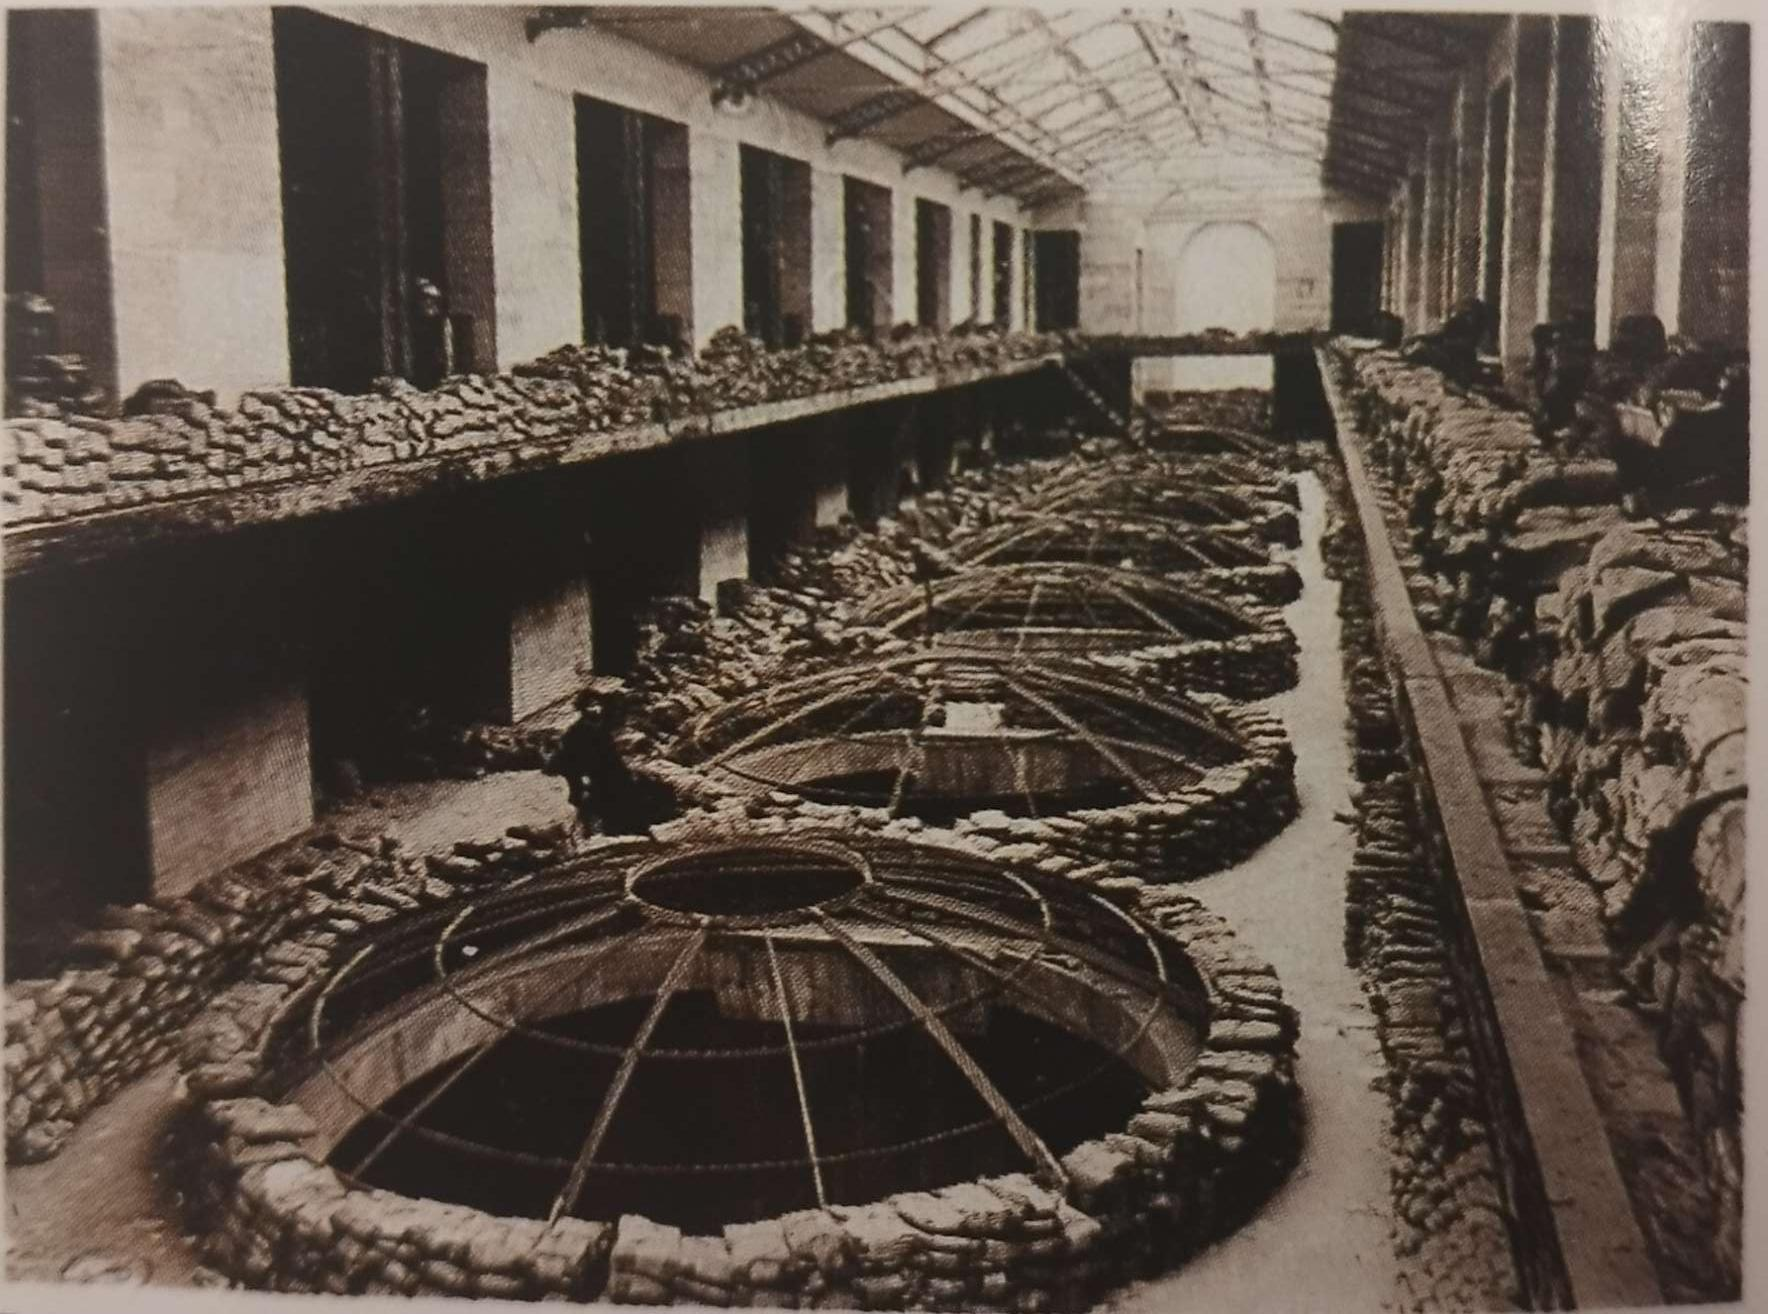
\includegraphics[width=0.75\linewidth]{Illustrations/1.jpg}
    \caption{Photo d'archive de la nef encombrée par les dossiers de la Cour des Comptes autour de 1900}
    \label{fig:placeholder}
\end{figure}

%%%%%%%%%%%%%%%%%%%%%%%%%%%%%%%%%%%%%%%%%%%%%%%%%%%%%%%%%%%%%%%%%%%%%%%%%%%%%%%%%%%%
%%%%%%%%%%%%%%%%%%%%%%%%%%%%%%%%%%%%%%%%%%%%%%%%%%%%%%%%%%%%%%%%%%%%%%%%%%%%%%%%%%%%
%%%%%%%%%%%%%%%%%%%%%%%%%%%%%%%%%%%%%%CHAPITRE%%%%%%%%%%%%%%%%%%%%%%%%%%%%%%%%%%%%%%
%%%%%%%%%%%%%%%%%%%%%%%%%%%%%%%%%%%%%%%%%%%%%%%%%%%%%%%%%%%%%%%%%%%%%%%%%%%%%%%%%%%%
%%%%%%%%%%%%%%%%%%%%%%%%%%%%%%%%%%%%%%%%%%%%%%%%%%%%%%%%%%%%%%%%%%%%%%%%%%%%%%%%%%%%

\chapter{Le XXe siècle, le Pavillon de Marsan et la gouvernance}

La nouvelle période qui s'ouvre pour l'UCAD avec l'accession aux locaux du Pavillon de Marsan et de l'aile de Rohan verra l'Union, le musée et sa bibliothèque se transformer. Leurs collections vont s'étendre et se patrimonialiser, et les publics vont progressivement changer à la faveur de cette patrimonialisation. Les artisans et dessinateurs seront peu à peu remplacés par les étudiants et amateurs d'arts. C'est aussi la période pendant laquelle les rapports entre l'État et l'UCAD vont se préciser et s'ancrer, au gré des luttes d'influences du pouvoir central et des manœuvres qu'entreprend l'association pour conserver son indépendance. Cette période verra pas moins de 5 conventions signées entre l'État et l'UCAD pour la concession du Pavillon de Marsan, avec par moments des changements structurels importants. Et \enquote{de convention en convention perdure ce statut si surprenant d'une collection nationale abritée dans des bâtiments de l'État, gérée grâce à une importante subvention publique, mais augmentée, restaurée, exposée et diffusée aux frais d'une association}\footnote{\cite{gady_dessin_2020}. p. 17.}.

\section{1905 : date fondatrice pour le musée et l'association}

Le 29 mai 1905, l'inauguration officielle du musée a lieu en présence du Président de la République Emile Loubet. Les sommes engagées pour les travaux de restauration par l'UCAD s'élèvent à 8 millions de francs. En réalité, une ouverture partielle depuis 1902 a permis au musée d'organiser ses premières expositions, mais son installation pleine et entière dans les locaux est retardée par la présence de centaines de milliers de liasses d'archives de la Cour des Comptes qui encombrent le pavillon de Marsan. 

\subsection{L'enrichissement des collections, méthodes d'acquisitions et donations}

Le statut loi 1901 de l'UCAD et sa reconnaissance d'utilité publique lui permettent de recevoir en plus des dons manuels, les legs et donations pour alimenter ses collections. Souvent les membres du Conseil d'administration sont aussi des donateurs à l'image de Jules Maciet, Paul Gasnault ou plus tard David David-Weill. Vient ensuite un legs d'importance pour les collections du musée, le legs Peyre. Puis, de façon générale, l'Union adopte une posture active dans l'achat d’œuvres pour alimenter ses collections. 

L'institution a cela de particulier qu'elle est aussi musée de séries d'objets et d'ensembles. Elle acquiert aussi des pièces uniques qui représentent leur temps ou une maîtrise particulière, mais le \textsc{xx}\textsuperscript{e}~siècle verra nombreuses manufactures, entreprises, ateliers, bijouteries donner en bloc des créations. Sans compter les ensembles constitués par les particuliers et collectionneurs qui cèdent leurs collections dans leurs testaments. C'est de cette manière que le Musée Camondo voit le jour le 21 décembre 1936 sous l'égide de l'UCAD. Le Comte Moïse de Camondo, en l'absence d'héritier, lègue un hôtel particulier, ses collections et des rentes suffisantes pour que soit édifié le Musée Nissim de Camondo, du nom de son fils défunt. 

Il faut aussi noter la procédure à laquelle l'association doit se soumettre afin de pouvoir accepter les dons et legs.

\vspace{1em}

\noindent
\hspace*{1cm}
\begin{minipage}{\dimexpr\linewidth-2cm}
\fontsize{10}{12}\selectfont
Les donations et les legs sont des types d’acquisitions pour lesquelles les dispositions doivent être authentifiées par des actes écrits. La donation est la transmission d’un bien à titre gratuit ; elle doit être passée devant notaire et acceptée par le bénéficiaire, à la différence du don, transmission moins procédurière qui n’engendre pas obligatoirement d’écrits. \footnotemark{}                                                     
\end{minipage}

\vspace{1em}

\footnotetext{\cite{siguret_ir_2001}. p. 29.}

 Ce point souligne par ailleurs l'un des problèmes principaux de nombreuses œuvres qui font partie des collections du musée : les artistes ou les manufactures qui donnent quantité d'ouvrages avec une simple note manuscrite indiquant par exemple \enquote{La manufacture Leroy donne un lot de papier peint.} 

Cela génère deux problèmes majeurs pour les conservateurs\wokisme trices, d'abord le manque de description du fonds, ce qui rend difficile le travail scientifique, puis le problème des droits qui surgit souvent dans ce genre de dons, où les descendant\wokisme e \wokisme s réclament des compensations dans le cas où les droits de publications ou de reproductions n'ont pas été spécifiquement accordés à l'institution. 
\vspace{1em}

\noindent
\hspace*{1cm}
\begin{minipage}{\dimexpr\linewidth-2cm}
\fontsize{10}{12}\selectfont
Le legs, lui, résulte de la disposition qu’une personne a stipulée dans son testament en faveur d’une (ou plusieurs) personne(s) morale(s) ou physique(s). Le légataire n’est pas obligé d’accepter le 
legs ; si c’est le cas, il doit prendre à sa charge les droits de succession inhérents. Pour les établissements reconnus d’utilité publique, l’acceptation d’une telle transmission doit être faite par les administrateurs (le président ou le trésorier de l’établissement). Elle est soumise à un contrôle gouvernemental.                                                       \footnotemark{}
\end{minipage}

\vspace{1em}

\footnotetext{\cite{siguret_ir_2001}. p. 29.}
 Ce contrôle gouvernemental se manifeste par des démarches administratives auxquelles doit se plier l'UCAD et dont le résultat est soumis à la volonté du préfet de la Seine, qui doit motiver son refus le cas échéant, et à un arrêté ministériel d'autorisation d'acceptation.

La grande générosité des donateurs, artistes et bienfaiteurs était parfois à double tranchant, ce qui apparaît dans la sous-série C3 : Donation et legs des archives du MAD. On y trouve des dossiers qui \enquote{révèlent parfois les difficultés que l’UCAD a éprouvées pour accepter des legs, et les démarches vaines de l’association pour se soustraire aux obligations financières trop lourdes qui lui incombaient en tant que légataire}\footnote{\cite{siguret_ir_2001}. p. 30.}.


\subsection{Les premières expositions et le rapport au public}

Au fil des acquisitions et des mutations des collections, l'idée d'un musée comme \enquote{conservatoire de l'Art décoratif} s'affirme\footnote{\cite{brunhammer_beau_1992}. p. 70.}. Le musée alterne entre deux types de collections qui dictent leur présentation et leur répartition : 

\vspace{1em}

\noindent
\hspace*{1cm}
\begin{minipage}{\dimexpr\linewidth-2cm}
\fontsize{10}{12}\selectfont
des séries d'objet classées suivant leur typologie, leur matière, leur provenance ou leur appartenance à une manufacture, une région, ou un pays, et des ensembles d’œuvres réunies de façon à restituer l'atmosphère d'une époque dans un lieu donnée.                                                        \footnotemark{}
\end{minipage}

\vspace{1em}

\footnotetext{\cite{brunhammer_beau_1992}. p. 73.}


 

De là, et de par la manière dont le musée s'est constitué et installé, il semble inévitable aux yeux des dirigeant de l'Union que le musée perde de sa valeur pédagogique initiale. Pourtant élément central du projet de l'association, les publics concernés par le musée sont de moins en moins les artisans et créateurs, et de plus en plus les collectionneurs et amateurs d'arts. Le projet muséal semble se diriger de plus en plus vers l'idée d'un \enquote{Conservatoire de l'Art décoratif}, de plus en plus loin de l'idée du pollinisateur de la création contemporaine qu'il voulait être\footnote{\cite{brunhammer_beau_1992}. p. 70.}. 

Ce sont les importants dons du début du \textsc{xx}\textsuperscript{e}~siècle qui motivent les thèmes des premières expositions avec les expositions sur le groupe de l'École de Nancy, l'Art musulman et les Primitifs français, respectivement en 1902, 1903 et 1904. Sur la période allant de l'ouverture du musée à la fin des années soixante on dénombre pas moins de 88 expositions organisées par l'Union, avec uniquement des coupures lors des deux Grandes Guerres Mondiales\footnote{\cite{noauthor__1970}. \enquote{\textit{Annexe 3 : 100 ans d'expositions à l'Union centrale}}}.

En dépit du déplacement du rôle de l'Union vers une tâche plus historique qu'instigatrice ou promotrice des techniques, elle continue de vouloir porter un rôle pédagogique et de formation. Elle crée en 1944 le Centre d'art et de techniques (CAT) qui deviendra l'École Camondo, une école de désign et d'architecture intérieure. Elle déplace ses volontés de formation vers la jeunesse et met en place une série d'initiatives ayant pour buts de sensibiliser la jeunesse, et de \enquote{former le goût des enfants au contact des objets d'arts, de diriger et de développer leur talents}\footnote{\cite{noauthor__1970}}. C'est l'ouverture des ateliers pour les moins de treize ans — qui deviendront les Ateliers du Carrousel, de la tenue de Conférences-promenades et de la création d'un Service éducatif qui mets à disposition des publics un service de documentation et de reproductions photographiques. 

\section{Les accords avec l'État et l'entrée au patrimoine public des collections}

À l’échéance de la première convention, en 1920, toutes les œuvres du musée et de la bibliothèque deviennent propriétés nationales. Cependant, les membres de l'Union n'entendent pas laisser désormais à des fonctionnaires la charge du musée et des collections constituées entièrement de dons et d'achats de passionnés qui, jusque-là, en avaient la gestion. \enquote{Sans parler des collectionneurs, qui confient plus volontiers leurs trésors à des mains privées qu'à l'État}\footnote{\cite{brunhammer_beau_1992}. p. 70.}. \hfill \break

Avant la période de tension que se révélera être la décennie 1970 pour les rapports entre État et UCAD, trois conventions sont signées pour renouveler la concession du Pavillon de Marsan et régir la gouvernance de l'Association, respectivement en 1920, 1935 et 1950. Dans la convention de 1920 apparaît pour la première fois la possibilité de prolonger la durée de la convention par simple décret, et le principe d'un partage des charges entre État et UCAD. L'UCAD a à sa charge l'entretien des locaux et l'organisation des expositions. L'État pour sa part prend en charge les dépenses relatives au personnel. Ce dernier point amorce un état de fait, toujours en cours de nos jours, qui veut que \enquote{l'effectif actuel du personnel de toutes catégories ne pourra être augmenté sans l'autorisation} du Ministère de la Culture et des Finances\footnote{\cite{noauthor__1970}}. Ce point ne soumet cependant pas le recrutement des personnels aux mêmes exigences que dans le secteur public, et l'Union est libre d'engager ou de renvoyer son personnel sans contrôle de l'État. De plus, 10 représentants de l'État font désormais partie du Conseil d'Administration de l'UCAD. 

Dans les conventions de 1935 et 1950, les seules modifications concernent la nombre de membres représentant de l'État qui passe de 10 à 15, mais aussi, désormais, l'État exige que \enquote{le personnel scientifique [soit] recruté parmi les candidats inscrits sur les listes d'aptitudes} par le pouvoir central\footnote{\cite{noauthor__1970}. \textit{Rapport sur le renouvellement... p. 4}.}.

\section{1970 et la redéfinition des rapports entre l'État et l'UCAD}

La convention qui devait être renouvelée en 1965 ne voit le jour que plusieurs années plus tard à la faveur d'âpres négociations entre le Ministère de la Culture et l'UCAD. C'est le cabinet du ministre André Malraux qui se charge d'examiner les demandes de l'association et d'arbitrer la situation compliquée qui s'est créée au fil du temps.

\subsection{Entre affirmation de l'État et demandes de l'UCAD}

La convention n'est signée qu'en 1975 pour une courte période de deux ans, puis en 1977 pour cinq ans, et pour cause, pendant la période, l'État tente de remettre la main sur l'ensemble du palais du Louvre pour en faire \enquote{le plus grand musée du monde}\footnote{\cite{brunhammer_beau_1992}. p. 92.}, mettant en danger l'existence même de l'UCAD. D'un côté l'Union demande à l'État de prendre en charge une plus grande part du personnel et des frais de fonctionnement, d'abandonner la disposition qui oblige l'UCAD à recruter parmi les candidats inscrits sur les listes d'aptitudes du Ministère, de revenir à une part de 10 administrateurs d'État et non pas 15 au Conseil d'Administration. Enfin l'UCAD veut pouvoir renouveler la convention pour 15 ans et étendre son emprise sur les bâtiments qui lui ont été dévolus. À cela, l'État rechigne en prévision d'une éventuelle future expropriation de l'UCAD au profit du Louvre, que ce soit pour la durée de la convention ou l'emprise sur les bâtiments qui rendrait un déménagement prochain inconcevable. 

L'État se retrouve à naviguer dans des eaux étroites entre volonté de contrôle, du fait des crédits accordés à l'UCAD, et flexibilité et indépendance du modèle associatif. Par l'intermédiaire du Directeur des Musées de France\footnote{\cite{noauthor__1971}}, l'État répond favorablement à l'allocation d'une subvention globale pour les personnels et frais de fonctionnement. Il accepte l'abandon du contrôle du recrutement. Il propose cependant la nomination d'un contrôleur administratif et financier en la personne d'un commissaire du Gouvernement affecté à la gestion de l'Union.

%%%%%%%%%%%%%%%%%%%%%%%%%%%%%%%%%%%%%%%%%%%%%%%%%%%%%%%%%%%%%%%%%%%%%%%%%%%%%%%%%%%%
%%%%%%%%%%%%%%%%%%%%%%%%%%%%%%%%%%%%%%%%%%%%%%%%%%%%%%%%%%%%%%%%%%%%%%%%%%%%%%%%%%%%
%%%%%%%%%%%%%%%%%%%%%%%%%%%%%%%%%%%%%%CHAPITRE%%%%%%%%%%%%%%%%%%%%%%%%%%%%%%%%%%%%%%
%%%%%%%%%%%%%%%%%%%%%%%%%%%%%%%%%%%%%%%%%%%%%%%%%%%%%%%%%%%%%%%%%%%%%%%%%%%%%%%%%%%%
%%%%%%%%%%%%%%%%%%%%%%%%%%%%%%%%%%%%%%%%%%%%%%%%%%%%%%%%%%%%%%%%%%%%%%%%%%%%%%%%%%%%

\chapter{De l’année 1982 à nos jours, transformations et modernisation}

L'année 1982 marque une rupture et une étape importante pour l'UCAD. La convention qui lie l'association à l'État vient d'être renouvelée au 3 mars 1981 et l'association reçoit de nouveau sa reconnaissance d'utilité publique. En 1983 le musée ferme pour un grand chantier de travaux et rouvre le 23 mai 1985\footnote{\cite{noauthor__2006}.}.

\section{Évolutions structurelles du musée }

L'UCAD revêt une forme nouvelle mais garde beaucoup des aspects qui font le cœur de son identité, notamment le lien avec le privé et les mécènes. Dans la nouvelle convention avec l'État est affirmée l'idée que le pouvoir central pourvoit aux besoins de fonctionnement de l'association en termes de locaux et de masse salariale, mais que c'est à l'Union de financer les expositions, les restaurations et les acquisitions. C'est ce qui donne lieu à une situation singulière, où, en part du total le mécénat et l'initiative privée, représentent autour de 12 à 15\% des produits de l'association. Dans le même temps c'est aussi le mécénat et l'initiative privée qui finance a plus de 80\%, et souvent entièrement, le montage des expositions : l'activité principale du musée. Cet état de fait, rend la planification et la programmation du musée difficile à prévoir bien à l'avance, comme c'est souvent le cas dans les musées publics, du fait de l'incertitude budgétaire qui règne, parfois jusqu'au dernier moment, pour la tenue d'une exposition\footnote{\textit{Propos recueillis auprès de Sébastien Quéquet, attaché de conservation en charge du fonds photographique}}.


\subsection{Les évolutions salariales et financières}

Pendant la période récente l'UCAD et plus spécifiquement le musée ont vu un certain nombre d'évolutions que nous avons pu retracer grâce aux archives et aux rapports d'activités produits par l'institution depuis le début de la décennie 1980. Tout d'abord, les dépenses de l'UCAD n'ont cessé d'augmenter au fil du temps, mais l'Union est le plus souvent à l'équilibre ou bien génère un léger excédent, comme nous pouvons voir ci-dessous.

\begin{figure}[H]
    \centering
    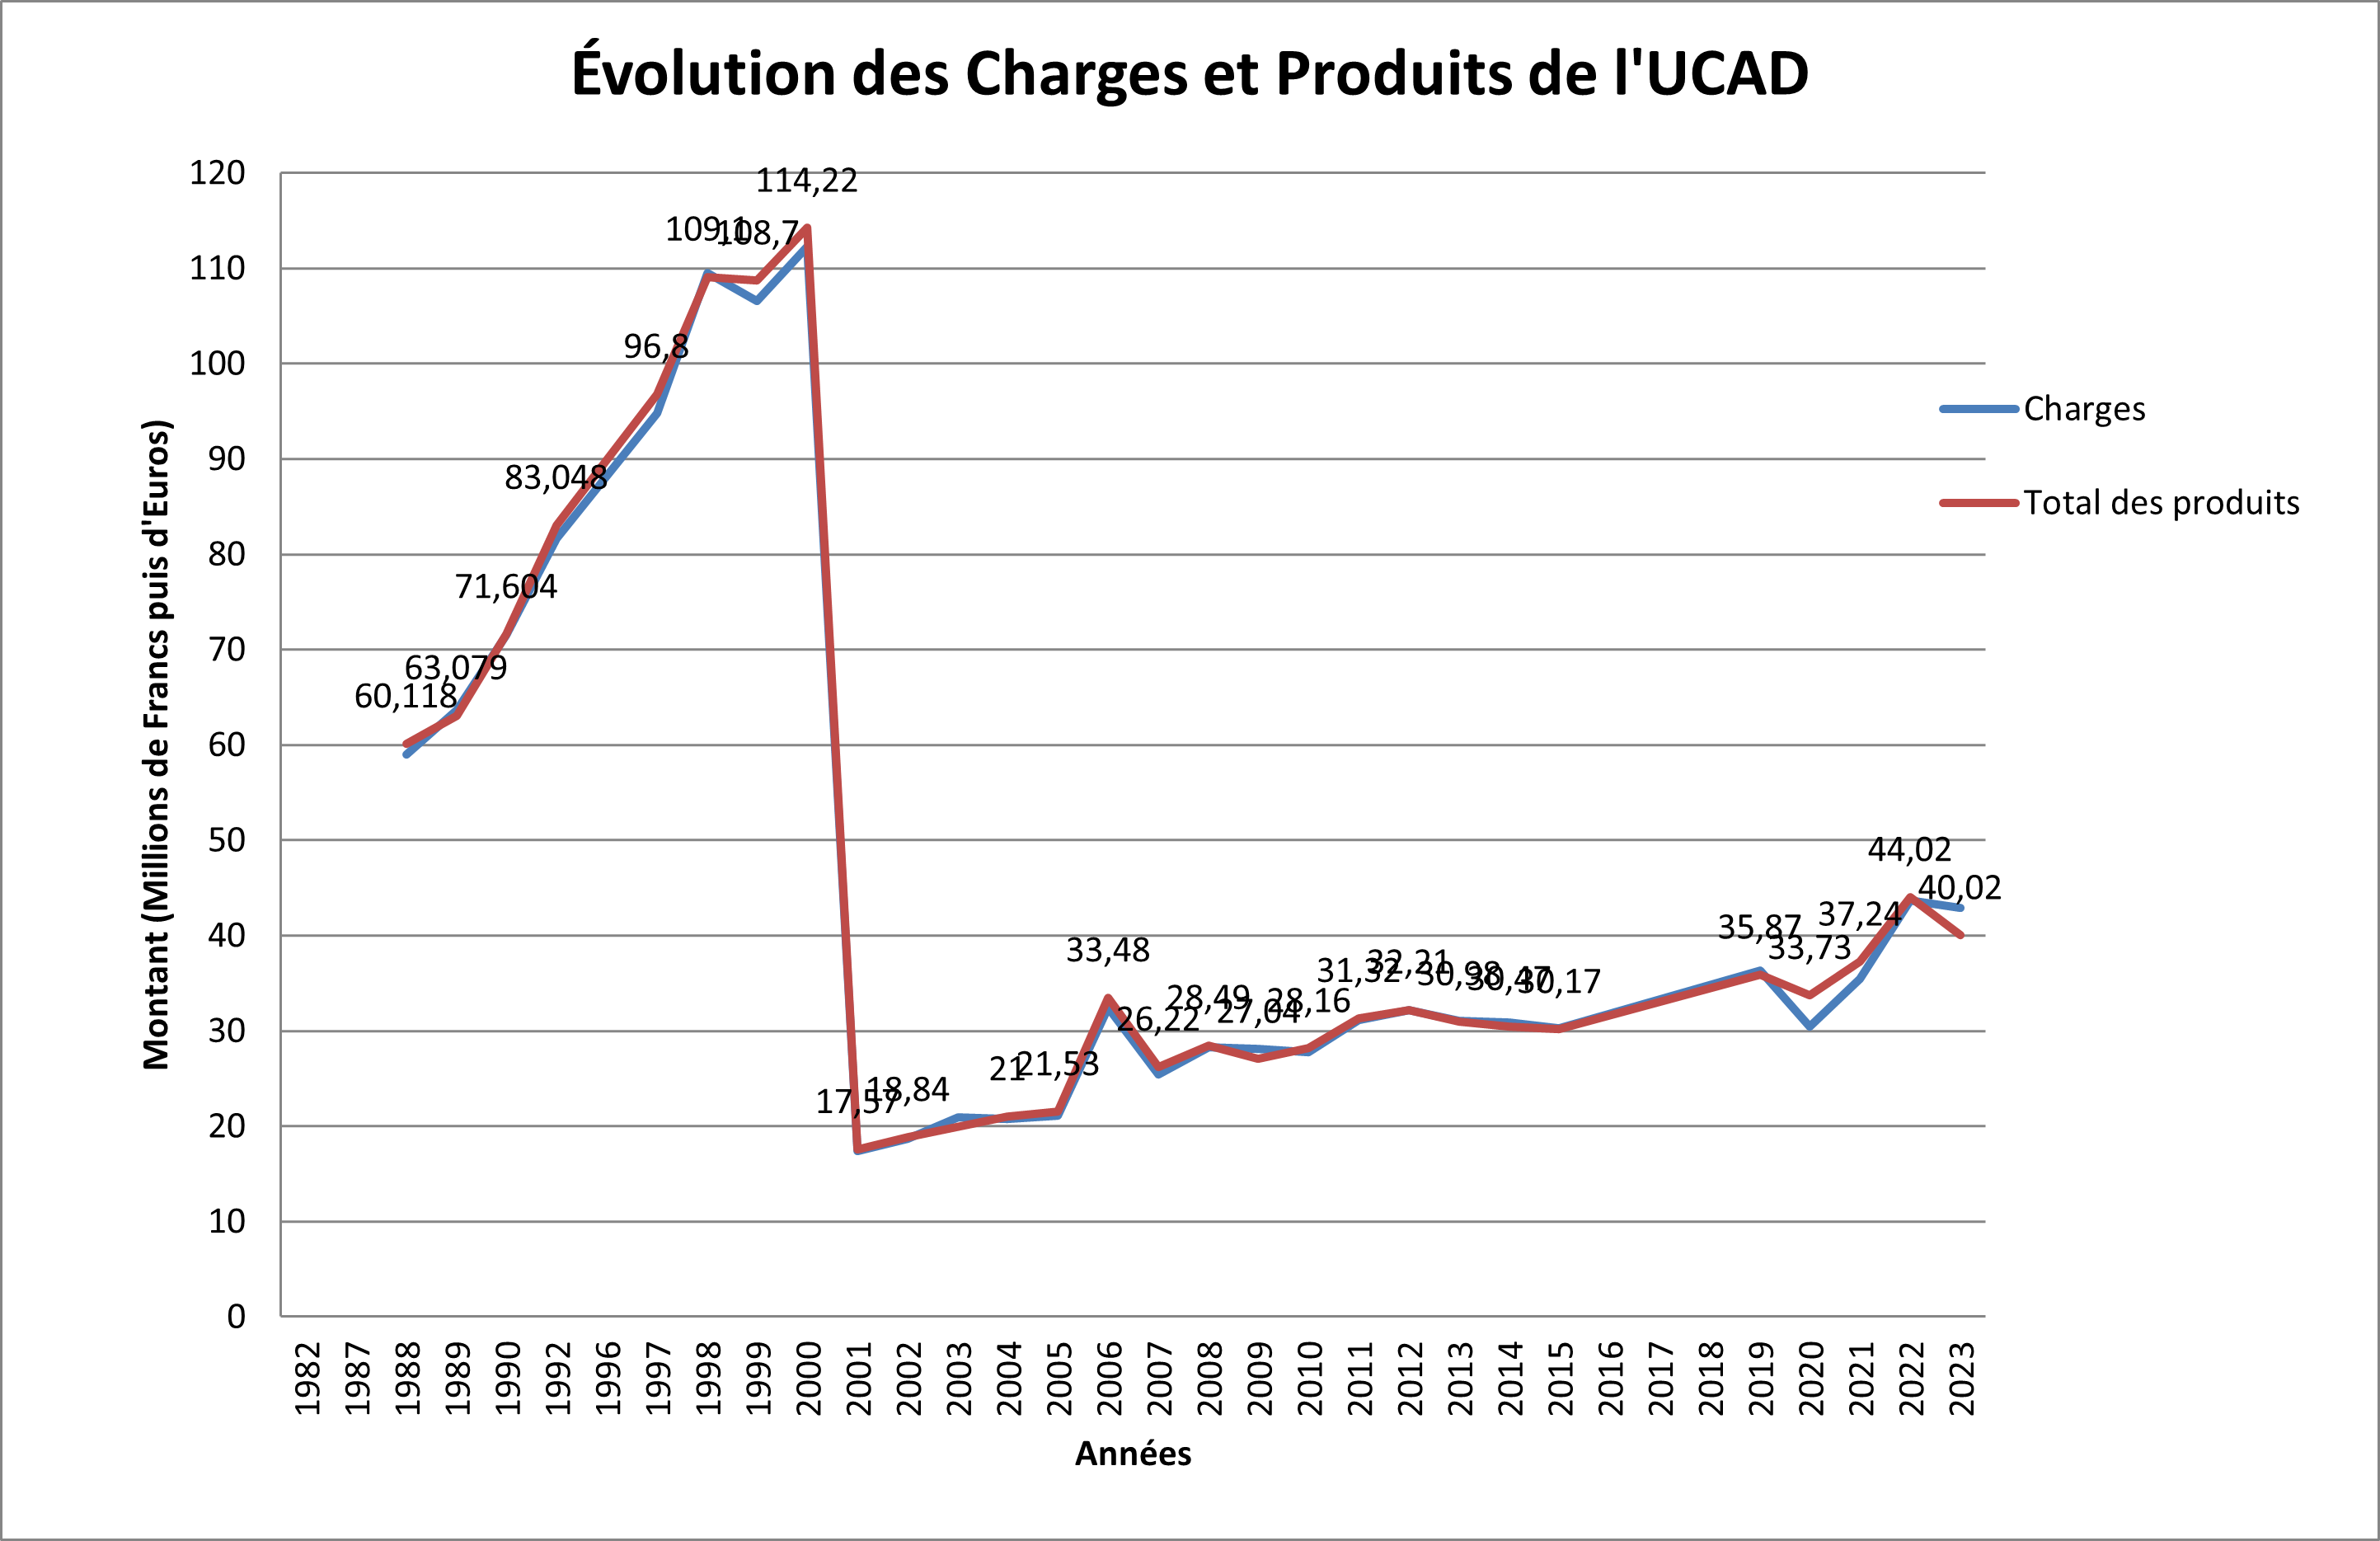
\includegraphics[width=0.75\linewidth]{Illustrations/Image1.png}
    \caption{Évolution des charges et des produits de l'Union entre 1982 et 2023}
    \label{fig:placeholder}
\end{figure}

\begin{figure}[H]
    \centering
    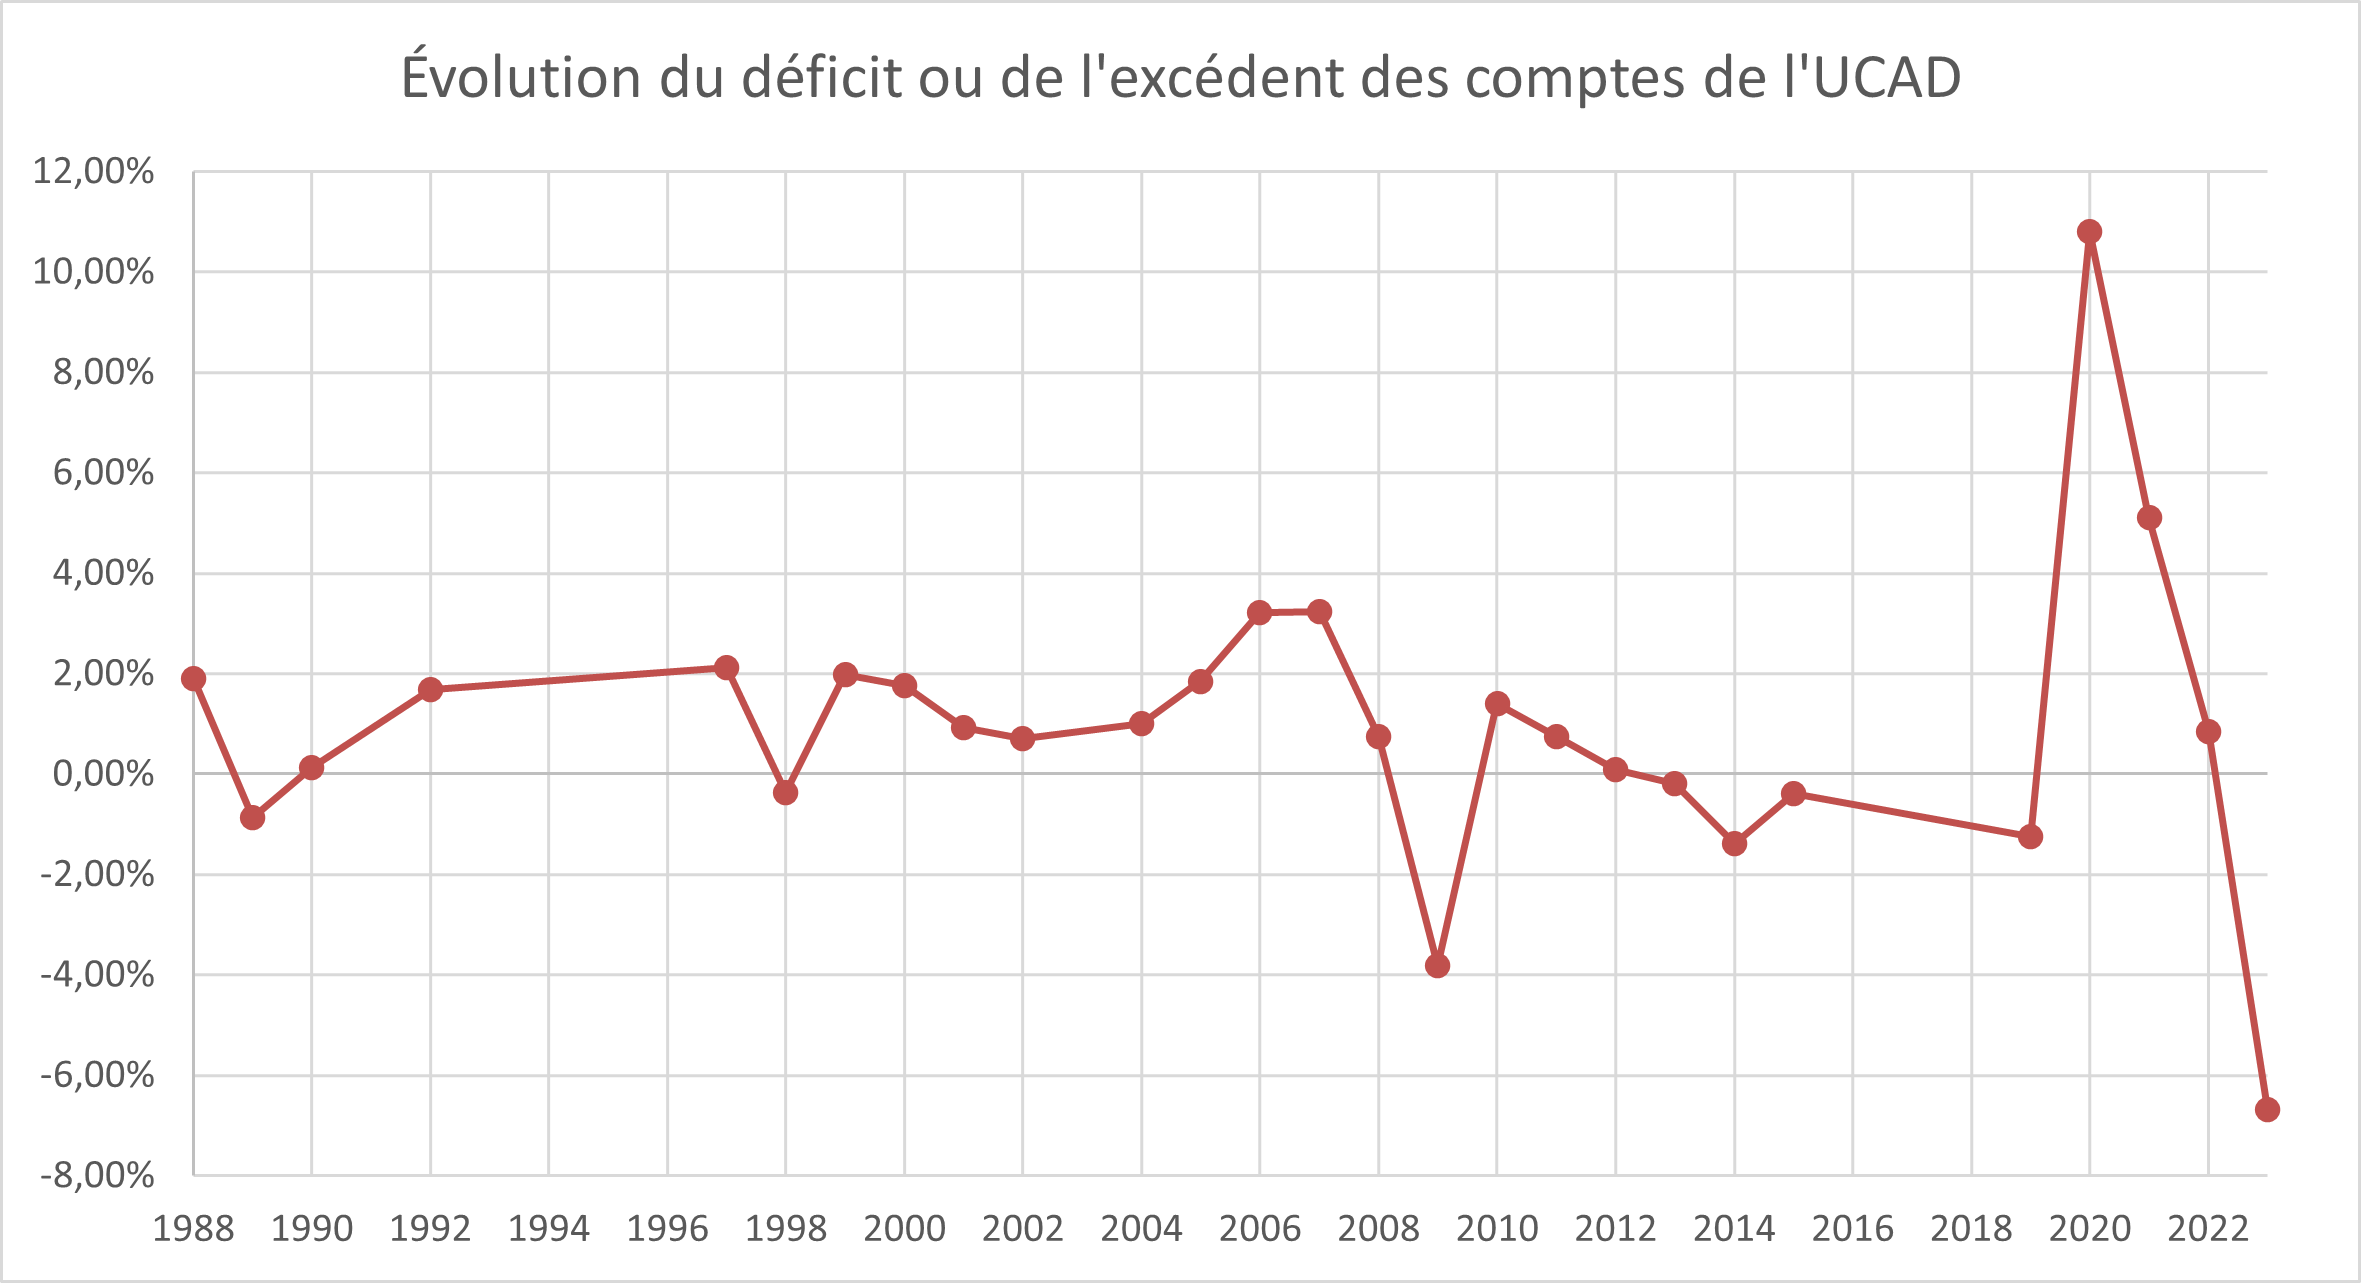
\includegraphics[width=0.75\linewidth]{Illustrations/Image5.png}
    \caption{Évolution du déficit et de l'excédent de l'Union entre 1988 et 2023}
    \label{fig:placeholder}
\end{figure}
\pagebreak

Ce qu'on observe c'est une augmentation croissante des coûts (114,22 millions de Francs étant équivalent à 17,69 millions d'Euros), qui ne se répercute pourtant pas visiblement sur la masse salariale, qui elle reste stable avec une moyenne de 306 employés entre 1982 et 2023\footnote{\cite{noauthor_convertisseur_nodate}}. Le balance entre total des produits et charges est plutôt bonne, avec 7 années enregistrant un déficit, notamment en 2009 des suites de la crise financière. Le large excédent de 2020 s'explique lui par les larges subventions exceptionnelles allouées par l'État au moment du COVID afin de faire face à la pandémie et à la cessation brutale des activités. 

\begin{figure}[H]
    \centering
    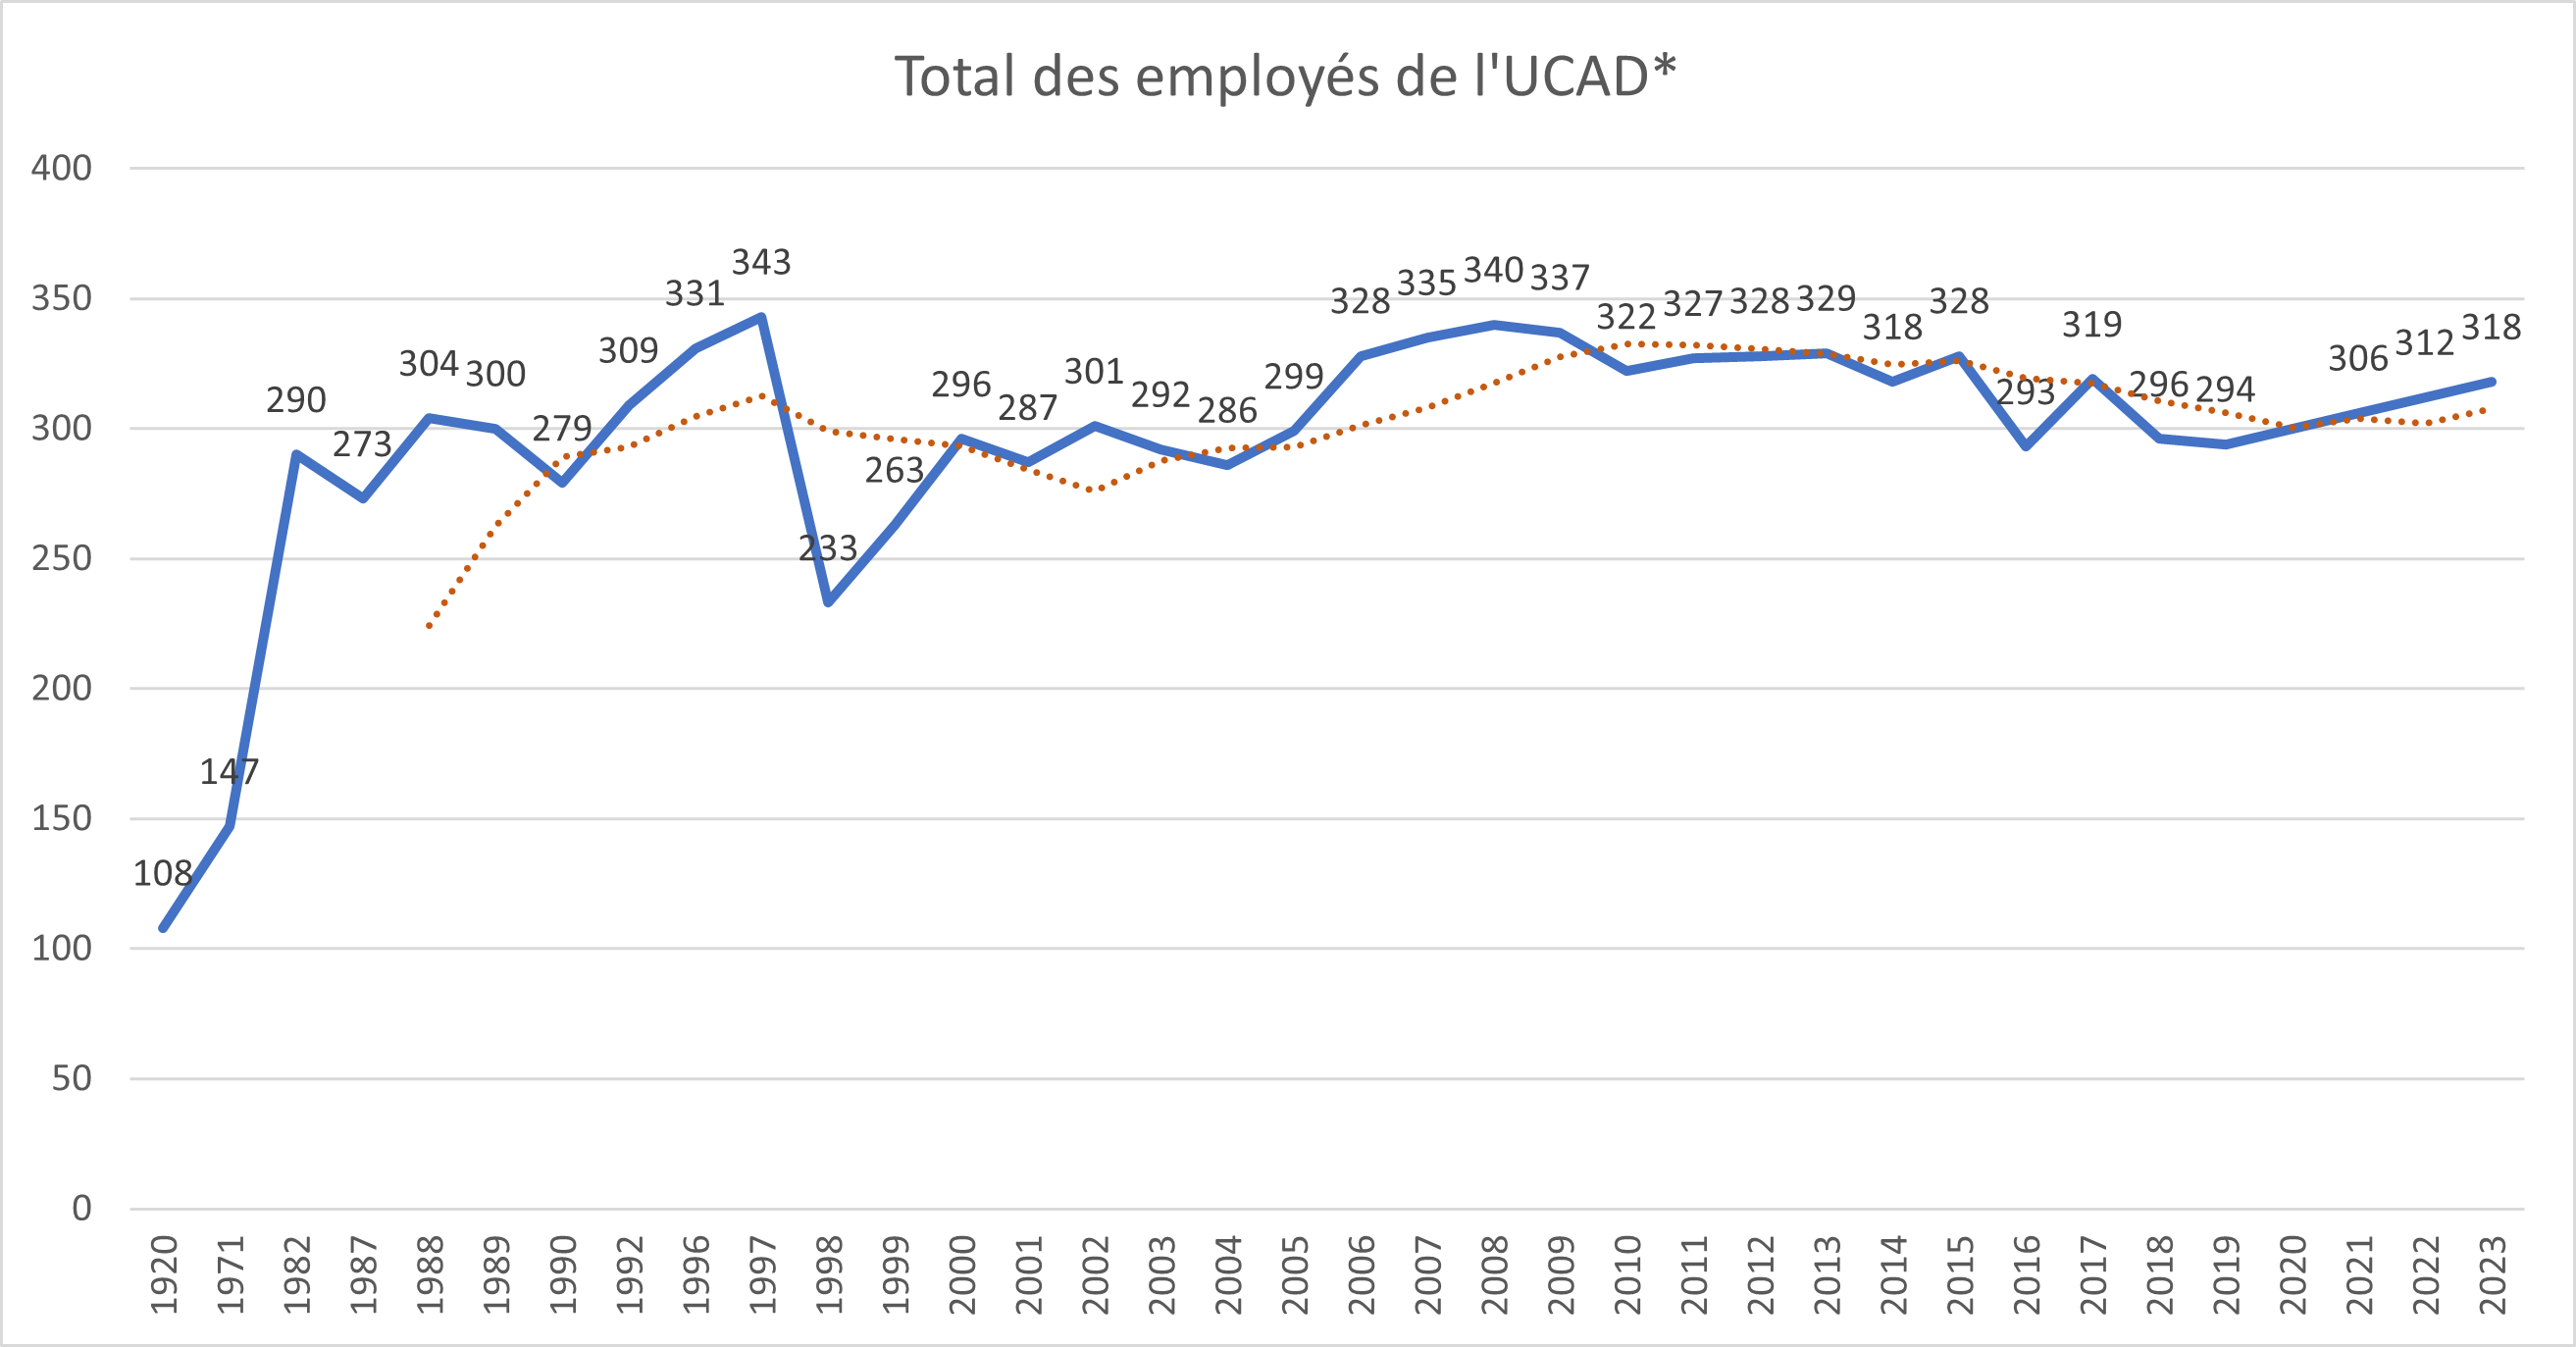
\includegraphics[width=0.75\linewidth]{Illustrations/Image8.png}
    \caption{Évolution du nombre d'employés de l'UCAD}
    \label{fig:placeholder}
\end{figure}

\textit{*Sauf secteurs non-conventionnés (Ateliers du Carrousel et École Camondo).}

Pour le cas qui nous intéresse particulièrement ici nous voulons nous pencher sur l'évolution des ressources humaines au sein du musée des Arts Décoratifs par rapport au reste de l'Union (à l'exclusion des secteurs non-conventionnés). Cela nous permet de quantifier aussi l'importance numérique en terme de répartition des moyens humains, que prend le musée. 

\begin{figure}[H]
    \centering
    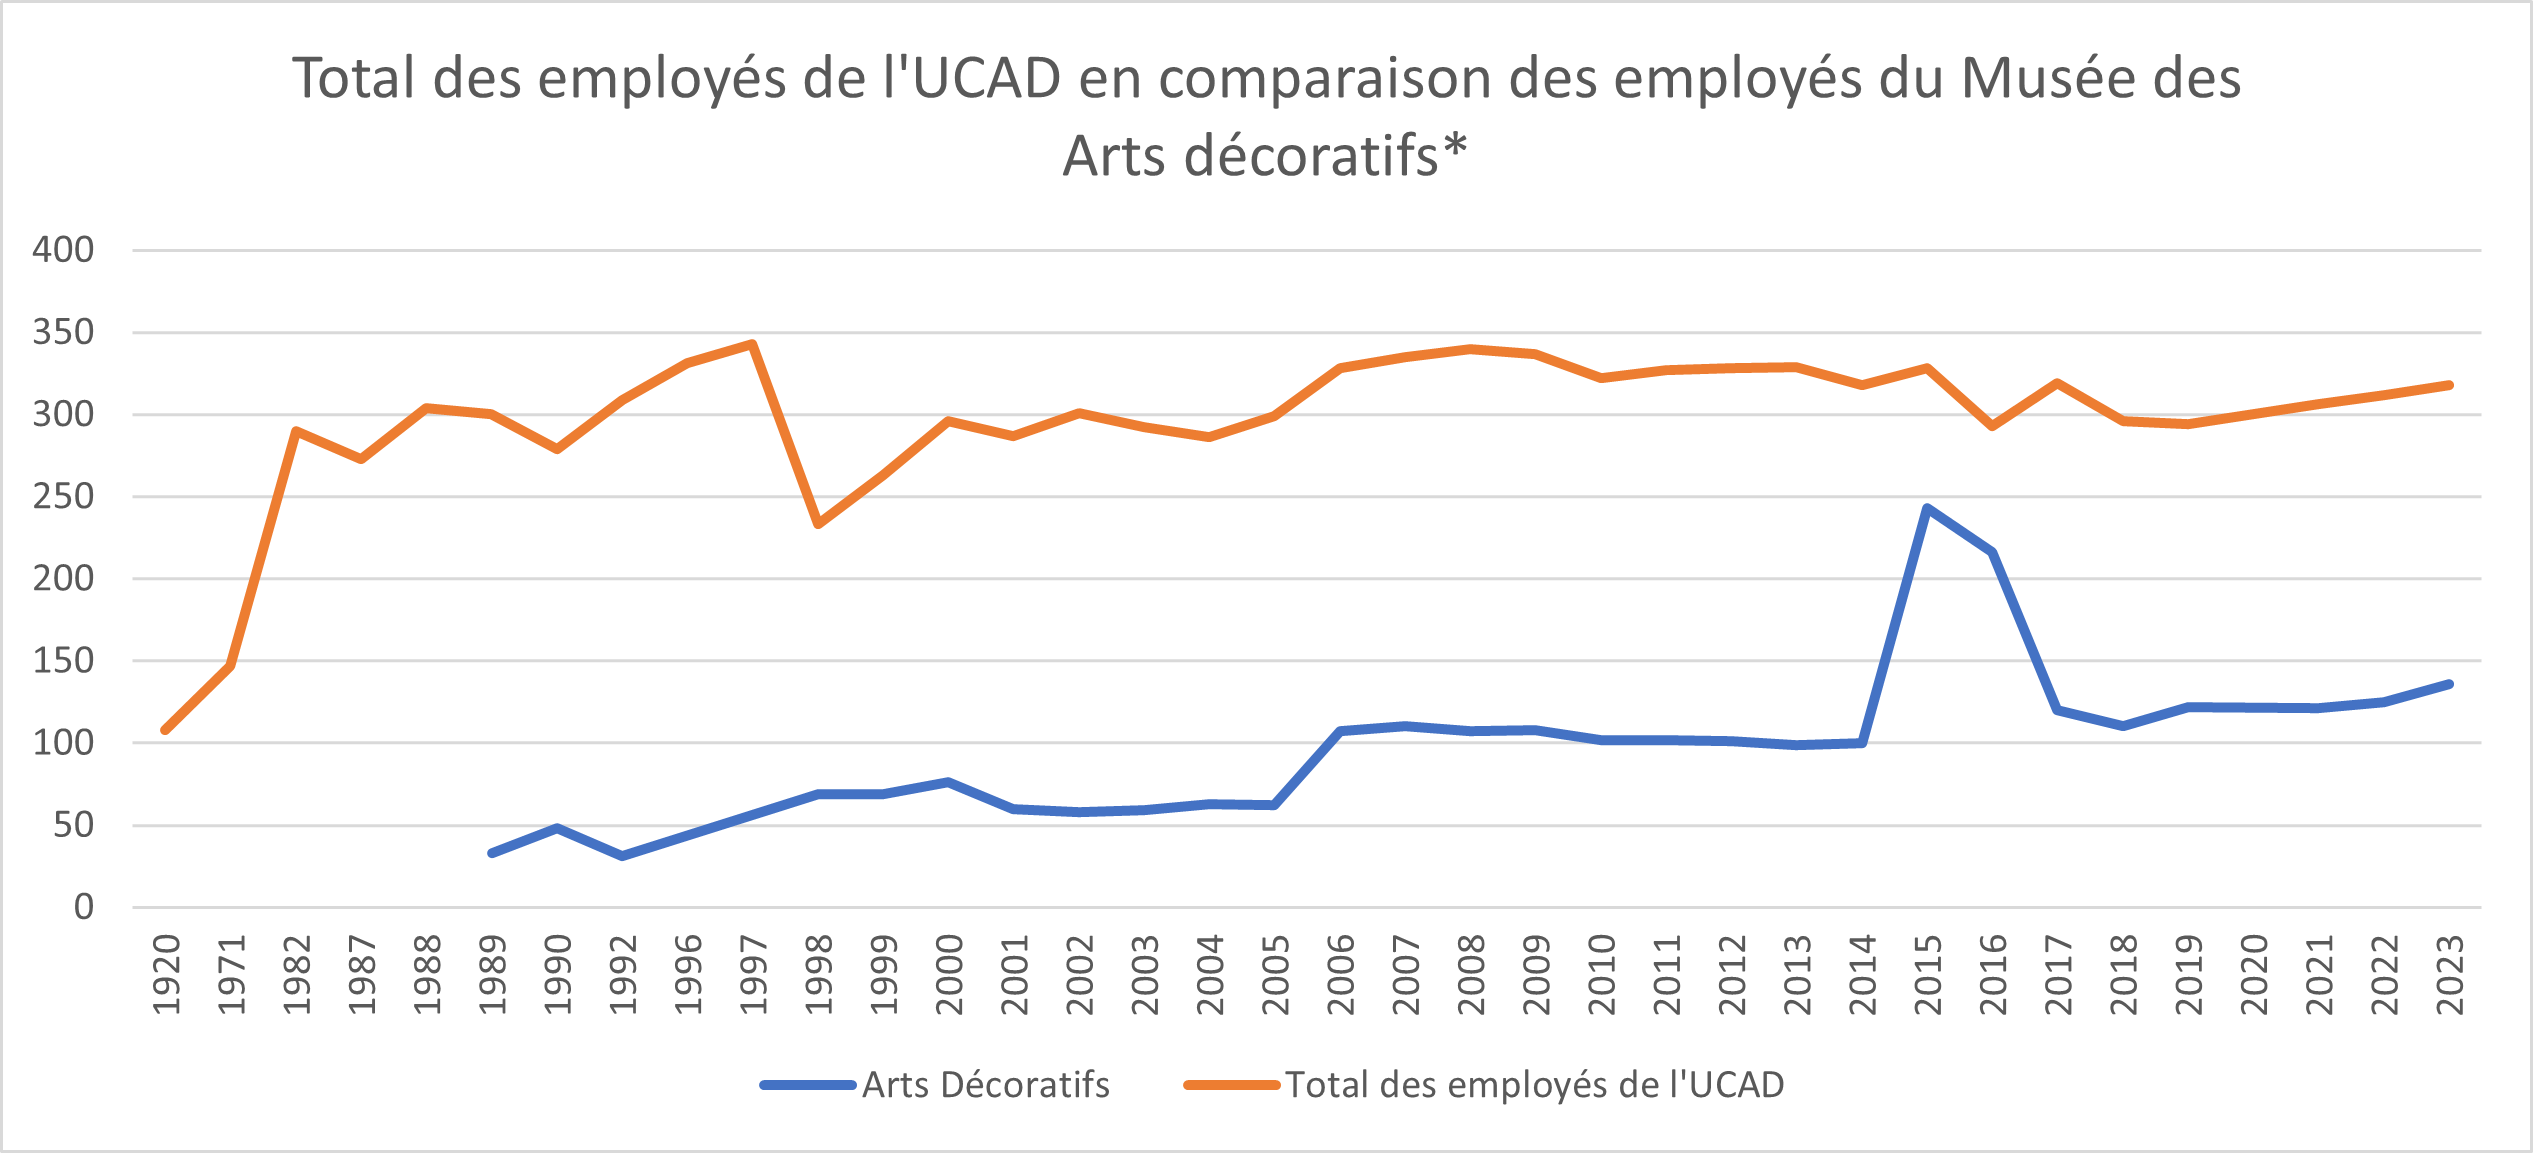
\includegraphics[width=0.75\linewidth]{Illustrations/Image10.png}
    \caption{Évolution des employés du musée des Arts Décoratifs comparé à l'ensemble du personnel entre 1989 et 2023}
    \label{fig:placeholder}
\end{figure}

Ce décompte spécifique pour le musée Arts décoratifs exclut les services techniques et les services communs des musées. Ce qu'on observe c'est que les Arts Décoratifs gagnent peu à peu en importance, notamment entre 2005 et 2006 où on observe presque un doublement des effectifs au musée. Cependant, le pic de 2015 s'explique par la fusion de tous les musées en une seule grande entité, ce qui regroupe tous les employé\wokisme e\wokisme s des musées sous la même appellation \enquote{Direction des musées} dans les sources postérieures. Les tendances à la baisse des années suivantes laissent apparaître une reconfiguration du partage salariale entre les corps de métiers au sein de l'Union, doublé d'une baisse générale de l'effectif entre 2015 et 2016. \hfill \break

\pagebreak

\begin{figure}[H]
    \centering
    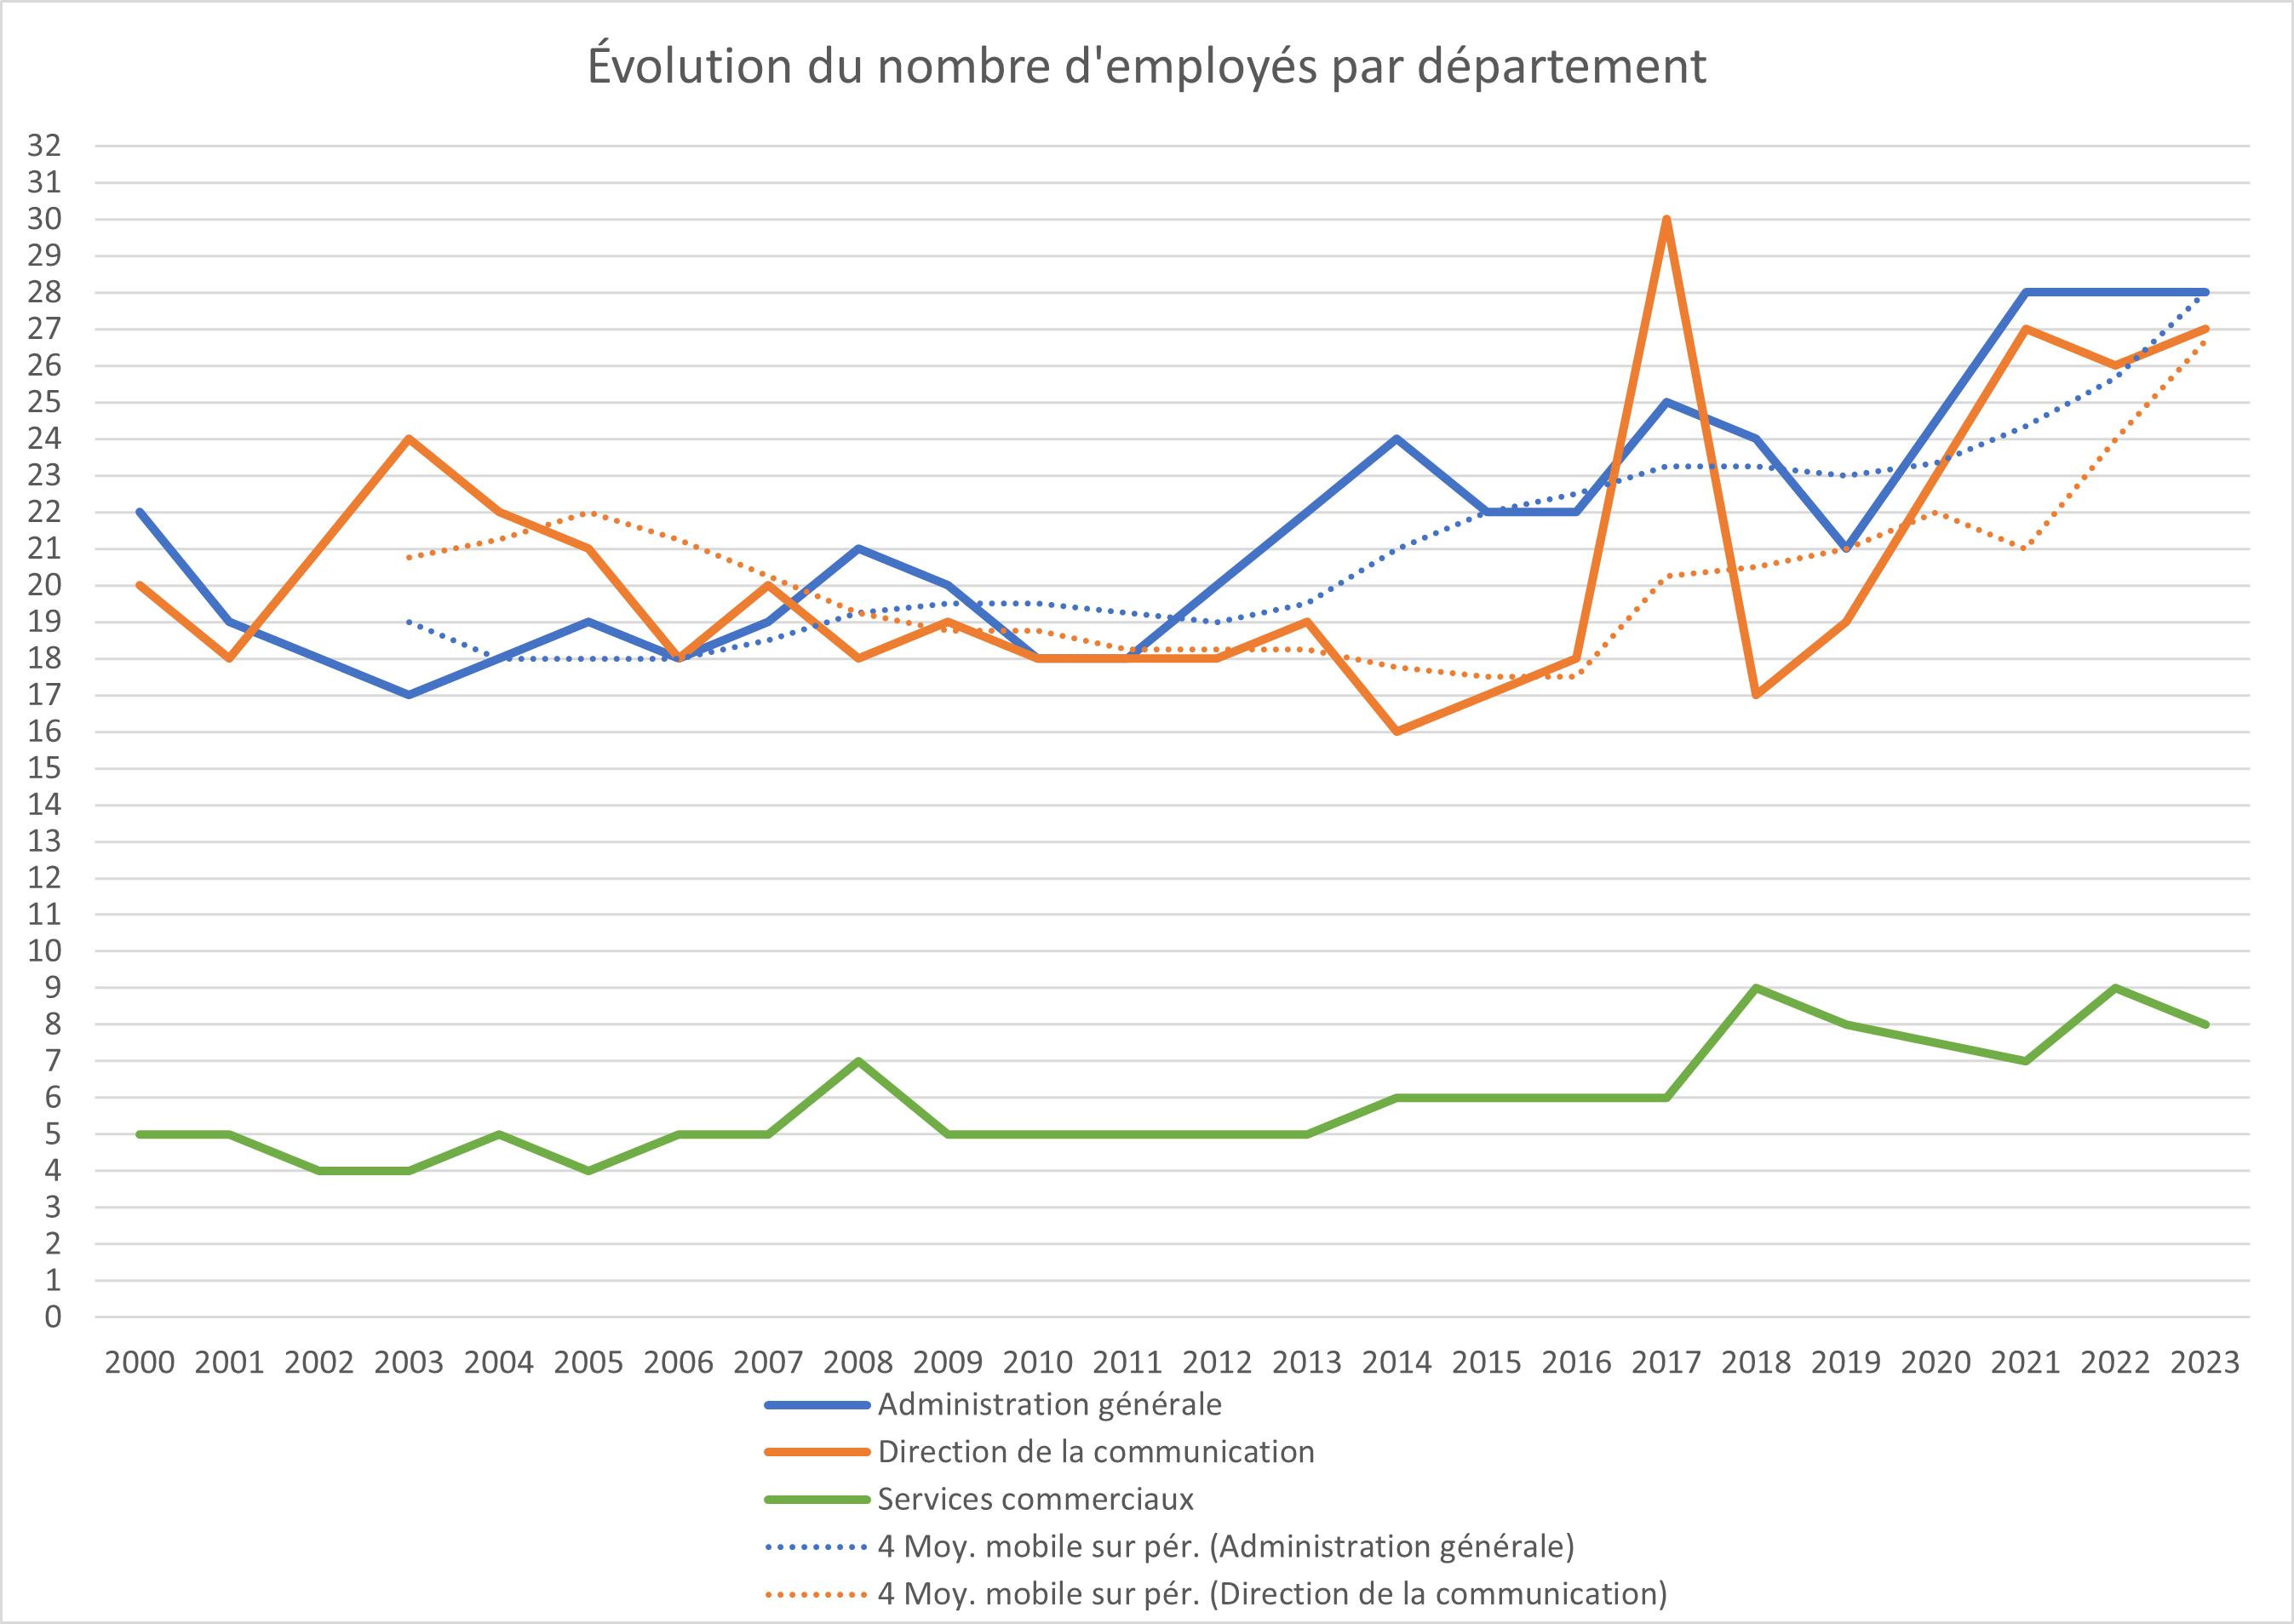
\includegraphics[width=0.75\linewidth]{Illustrations/Image12.png}
    \caption{Évolution du nombre d'employés par départements entre 2000 et 2023}
    \label{fig:placeholder}
\end{figure}

Cette reconfiguration des services du musée s'accompagne d'une tendance d'embauche à la hausse dans les secteurs commerciaux, de la communication et dans la direction. Cependant, ce qui n'apparaît pas ici dans nos visualisations, et qui pourtant est présent dans les rapports d'activités est la répartition entre C.D.I. et C.D.D. au sein de l'Union. Apparaît aussi dans les sources les pourcentages des employé\wokisme e\wokisme s par ancienneté et tranches d'âges, qui pourraient constituer une étude à part entière\footnote{\cite{noauthor__1982}}. Pour ce qui est est de la répartition entre contrats courts et contrats longue durée on observe une augmentation très nette du recours au C.D.D. entre 2010 et 2023 par rapport aux périodes précédentes. Entre 2000 et 2009 on passe de 17 à 27 employé\wokisme e\wokisme s en C.D.D., avec une moyenne autour de 19 sur la période. En 2010, on dénombre 15 employé\wokisme e\wokisme s en C.D.D. contre 51 en 2023, ce qui représente une hausse de 240\% du recours au C.D.D. dans l'Union (à l'exception des secteurs non-conventionnés), avec une moyenne de 35 C.D.D. Du côté des C.D.I., on trouve 302 employé\wokisme e\wokisme s en contrats longue durée en 2010, contre 261 en 2023, soit une baisse de 13,6\%. Si on compare avec la masse salariale totale, les deux années 2010 et 2023 sont plutôt proches avec 322 employé\wokisme e\wokisme s en tout en 2010 et 318 en 2023. 

Ces changements dans la gestion et la précarisation des postes est peut-être à mettre en rapport avec le fait que sur la période concernée (2010-2023), l'Union enregistre 5 des 7 années déficitaires sur ses comptes entre 1988 et 2023. Pourtant quand on observe avec le schéma ci-dessous cela correspond à une période où l'Union se finance en majorité à l'exception des années 2019 à 2022, en gardant bien à l'esprit que cette période correspond aussi à un moment exceptionnel avec les subventions liées au COVID. 

\begin{figure}[H]
    \centering
    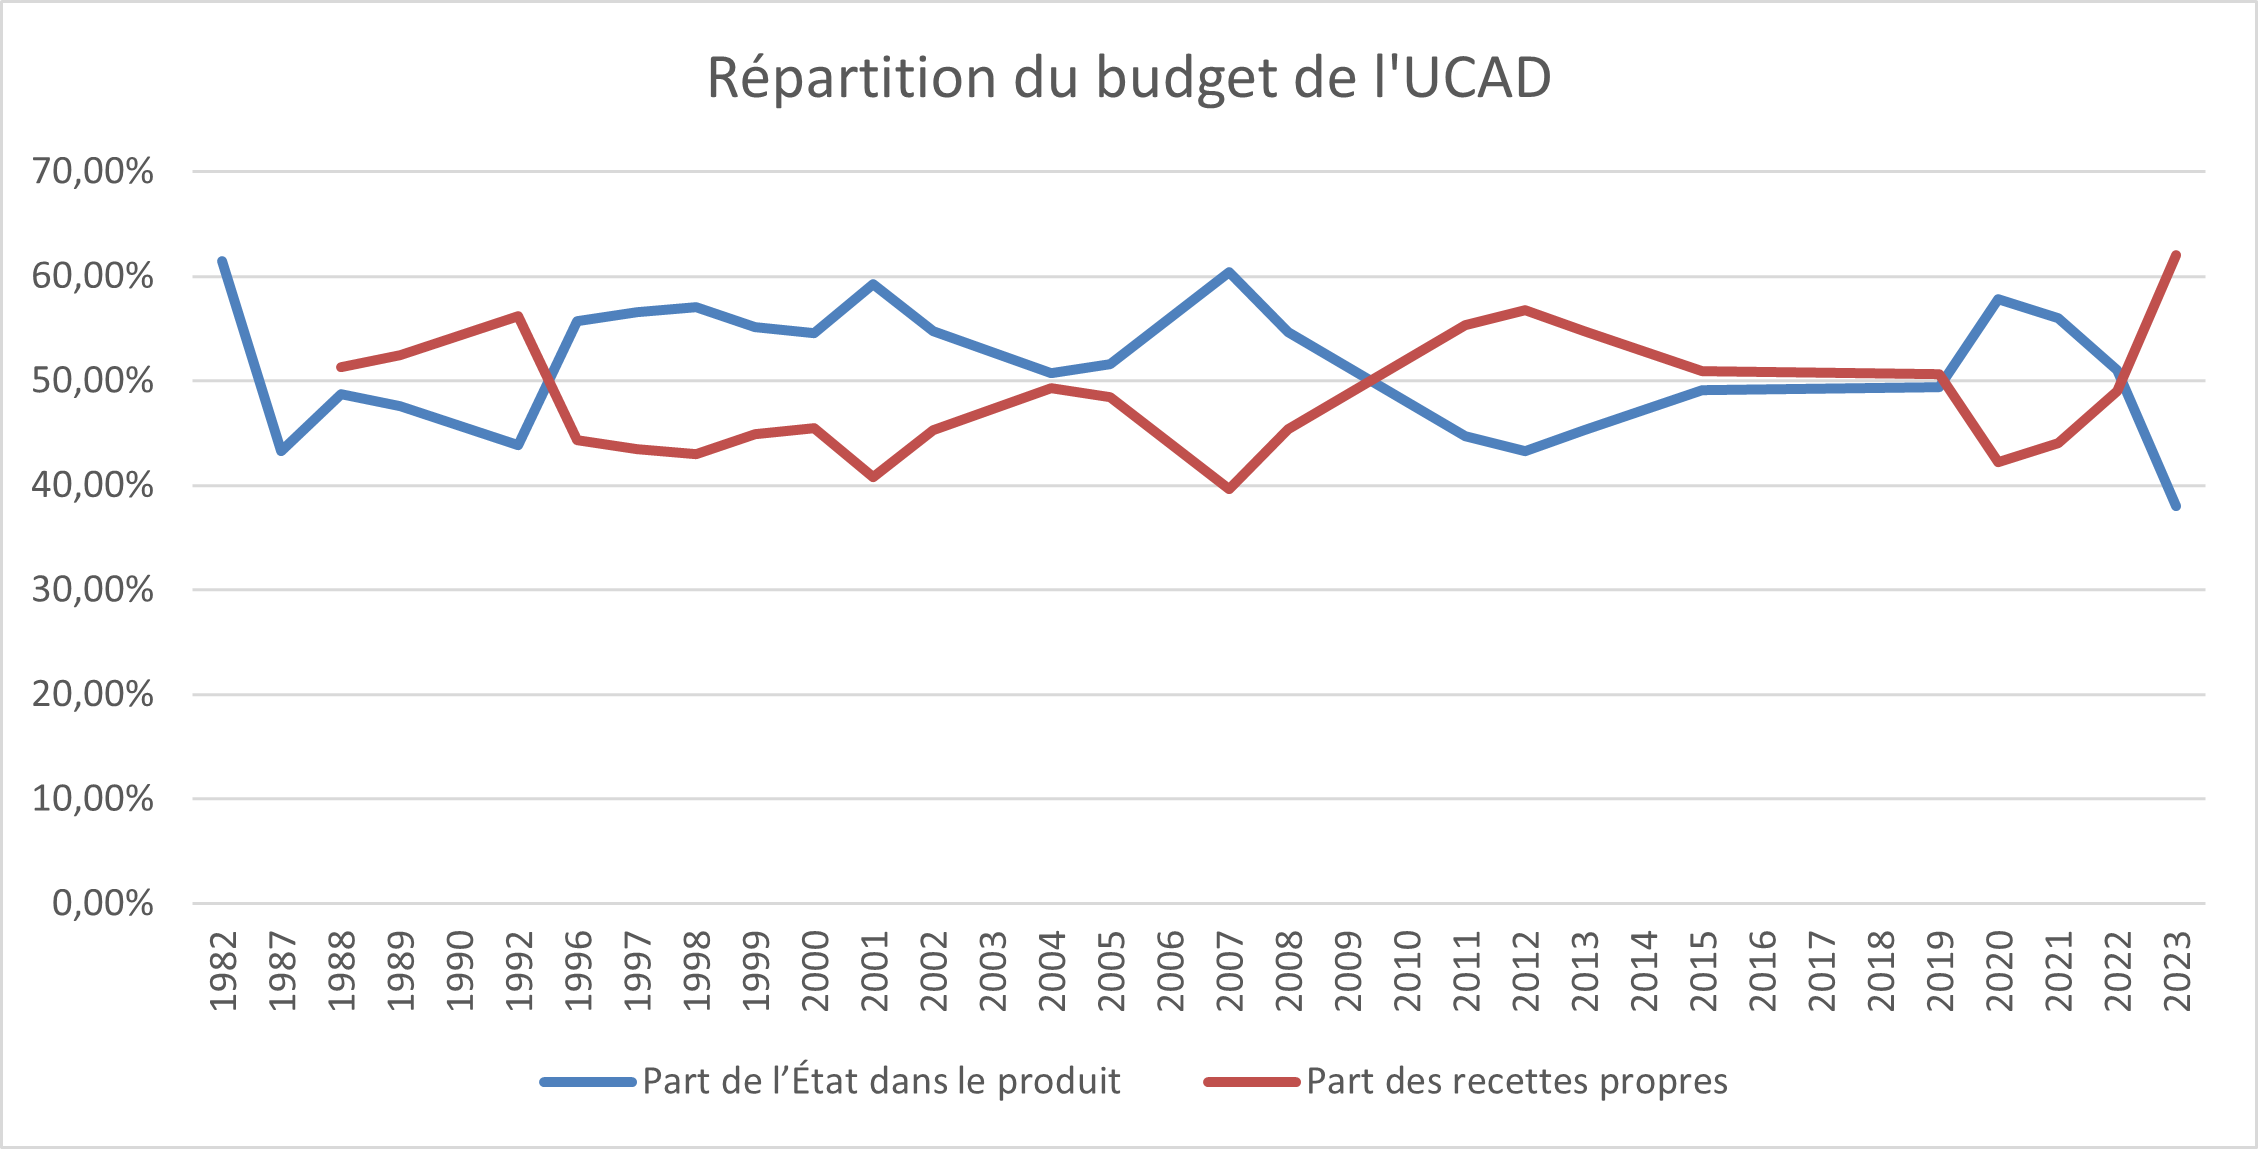
\includegraphics[width=0.75\linewidth]{Illustrations/Image2.png}
    \caption{Évolution de la part de l'État et des revenus propres de l'UCAD dans le total des produits entre 1982 et 2023}
    \label{fig:placeholder}
\end{figure}

\begin{figure}[H]
    \centering
    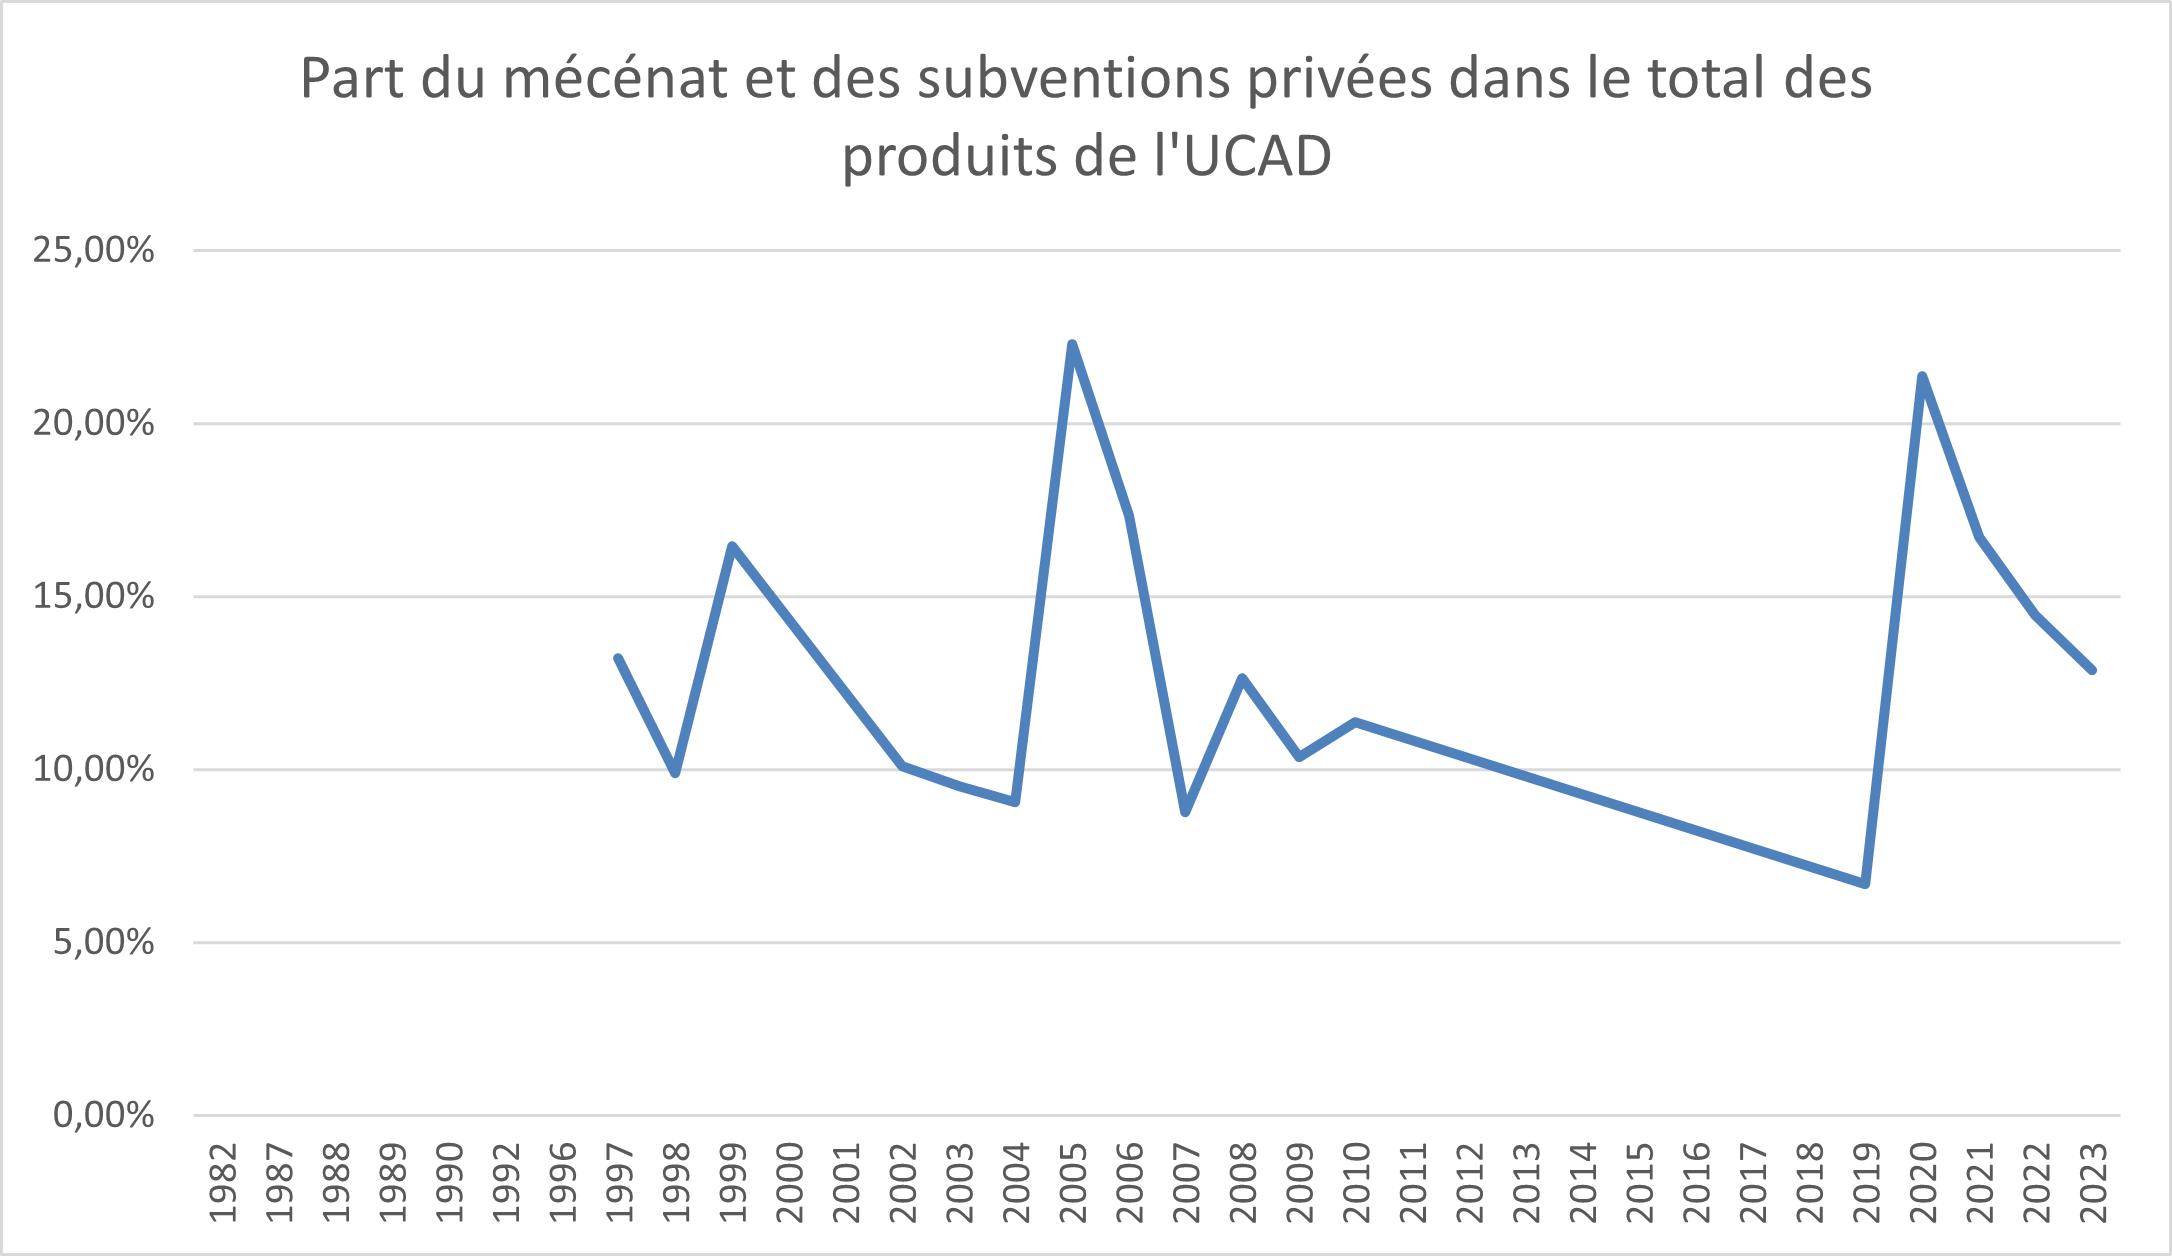
\includegraphics[width=0.75\linewidth]{Illustrations/Image3.png}
    \caption{Évolution en pourcentage de la part du mécénat et des revenus des privatisations sur les recettes propres de l'Union entre 1997 et 2023}
    \label{fig:placeholder}
\end{figure}

Enfin, si on prend en compte cette dernière visualisation, nous pouvons peut-être mettre en rapport cette tendance avec la baisse du mécénat et des revenus issus des privatisations sur la même période. Souvent, les postes liés à des expositions, ou à des chantiers de collections, de restauration ou de réhabilitations, sont des postes mécénés comme le prévoit la convention qui lie l'État à l'UCAD. Aussi, il est bon de souligner qu'en vertu de ladite convention, c'est l'État qui contrôle le plafond d'emploi de l'Union et qui dicte le nombre de postes permanent auxquels l'association peut pourvoir. Les raisons de cette baisse peuvent donc aussi être plus largement politiques et conjoncturelles, au gré des nominations au Ministère de la Culture ou des budgets votés à l'Assemblée, mais pour déterminer cela une étude approfondie serait nécessaire, nous ne pouvons avancer ici que des pistes non vérifiées. 

Pour conclure, nous voulons évoquer un état de fait éloquent posé en 1991 par le Directeur de l'Union d'alors, Antoine Riboud, au cours d'un entretien accordé au Monde. Ce qu'il évoque, après deux années à la tête de l'Union, représente une partie des spécificités structurante de l'UCAD : \enquote{Globalement, le bilan est très positif. L'UCAD regroupe des musées, des écoles qui tous vivent très pauvrement. Le personnel n'a pas le même salaire que celui du Louvre. La conservation est peu nombreuse, dévouée, mais très compartimentée. C'est une entreprise qui a besoin de se moderniser, d'évoluer. Pendant un an, il a fallu s'assurer qu'on restait bien rue de Rivoli. Nous avons, finalement, eu gain de cause}\footnote{\cite{noauthor_entretien_1991}}. Cette citation illustre bien, en effet, le constant danger qui plane au dessus de l'institution, de n'être pas renouvelée au Pavillon de Marsan et dans l'aile Rohan, le manque de moyens structurels en comparaison d'autres institutions patrimoniales publiques et l'aspect pluriel et fragmenté de l'institution. C'est ce dernier aspect, et les évolutions organisationnelles en termes de système d'information et de gouvernance mis en place au musée que nous allons étudier dans la fin du présent chapitre afin de rendre compte, aussi fidèlement que possible de l'état de l'organisation actuelle.

\section{De nouveaux musées et de nouveaux services}

L'histoire des musées qui composent désormais le MAD remonte un peu avant le début de notre période avec l'apparition de deux entités dans l'escarcelle des Arts décoratifs. En 1978 est inauguré le musée de l'affiche\footnote{\cite{siguret_ir_2001}. p. 1.}. Il est basé sur l'ancien fonds d'affiches de la bibliothèque des arts décoratifs, et son domaine d'activité est étendu. Il sera rebaptisé Musée de la publicité et transféré dans l'aile Rohan en 1999. De même le Centre national d'information et de documentation sur les métiers d'art (CNIDMA), est inauguré en 1974 et incorporé au musée des arts décoratifs comme département dès 1990. Pendant notre période, en 1986 est inauguré le musée des arts de la mode, fruit d'une collaboration entre l'UCAD et l'Union française des arts du costume. Il rouvre ses portes en 1997 sous le nom de musée de la mode et du textile. Toutes ces entités séparés viendront fusionner dans un même musée regroupant toutes les anciennes composantes en 2015. C'est de cette structuration qu'hérite le système d'information actuel. Les données des différentes collections reflètent encore souvent cette répartition dans les bases du musée. Il n'est pas rare de retrouver les noms de ces anciennes institutions en en-tête des dossiers et des classifications. La fusion a eu pour effet de tout regrouper sur un faible nombre de volumes, il existe 2 volumes principaux à l'heure actuelle, qui regroupent l'ensemble des données du musée avant 2020-2021. De cette histoire naturelle des institutions et des enjeux techniques contemporains, sont nées plusieurs problématiques et états de fait qu'il est important de garder à l'esprit dans le cadre de notre étude. L'état des fonds, la dispersion des informations et le système d'information telle qu'il s'est développé sont autant de paramètres à prendre en compte pour le déploiement et la pérennisation de nouvelles méthodes de traitements au sein du musée. 

C'est la raison pour laquelle nous voulons revenir sur l'histoire du déploiement des systèmes informatiques au sein du musée, afin de contextualiser et de remettre en perspective les enjeux passés et présents qui encadrent les collections et leur gestion. Nous allons aussi, dans un second et dernier temps, revenir quelque peu sur l'histoire récente de la bibliothèque et du service d'archives afin de mettre en lumière une autre partie des problèmes qui se posent aujourd'hui aux conservateurs tant des musées et des bibliothèques. 

\subsection{L'informatisation croissante}

Les premières réflexions autour de la nécessité d'informatiser les collections émergent dès le début des années 1990. On en retrouve des traces dans les archives de l'UCAD : \enquote{Les études préalables à l'informatisation des collections sont engagées pour démarrer en 1991}\footnote{\cite{noauthor__1991}. p. 8.}. Le président de l'UCAD évoque aussi ce chantier et la première difficulté qu'il rencontre : le manque de moyens. À la question \enquote{Quel intérêt accordez-vous à la conservation ?}, il répond : \enquote{La première chose à faire, c'est de mettre nos collections sur ordinateur, pour estimer nos richesses. Cette informatisation demandera des moyens importants qui devront figurer dans notre budget de fonctionnement}\footnote{\cite{noauthor_entretien_1991}}. Outre une vision, peut-être partielle des enjeux de conservation, il souligne un point important : être en mesure de pleinement comptabiliser tout ce qui se trouve dans les collections de l'Union. En avril 1996 est lancé la présence de l'UCAD sur internet, la même année on voit la mise en place du premier réseau interne à l'Union qui permet d'accéder aux fiches des œuvres, aux notices de la bibliothèque et, après harmonisation, aux fonds des centres documentaires\footnote{\cite{noauthor__1996}. p. 11 et 13.}. 

Durant les années qui suivent, le parc informatique se développe, les différentes institutions, qui composent l'Union, sont progressivement connectées à internet. Au début des années 2000, un logiciel de gestion de parc informatique est mis en place et les premières campagnes de numérisation massive des albums Maciet ont lieu, pour permettre aux usagers de la bibliothèque de les consulter sur des postes ou sur internet\footnote{\cite{noauthor__1982}. Rapport 2002, p. 54-55.}. Les services informatiques sont aussi sollicités, pendant la première décennie des années 2000, dans divers projets multimédias, de réalisation de documentaire ou de films sur les expositions et leur préparation. En 2010, le SI prépare la mise en ligne des collections. L'année 2020 est une année charnière pour comprendre l'état du système d'information actuel, des documents et des collections du MAD de nos jours. Avec le confinement, et la nécessité de passer en distanciel les activités, le MAD a été massivement basculé sur la suite Microsoft Teams pour continuer ses activités, ce qui a eu pour effet de fragmenter l'information entre des groupes par département et de confier toutes les données du musée à un acteur américain. En plus du coût, l'export vers Teams a eu comme conséquence d'effacer une partie des métadonnées des fichiers au moment de l'import, ce qui pose un certain nombre de problèmes actuellement, notamment pour le service d'archives. 

L'autre grand changement cette année-là est la reprise du chantier \enquote{de changement du système de gestion et de publication des collections et des archives du musée}\footnote{\cite{noauthor__1982}. Rapport d'activités 2020, p. 68.}. Ce travail a donné lieu à une définition de l'architecture cible et à un état des lieux des médias. C'est ce travail qui a amené à la mise en place d'un contrat avec Skinsoft pour la mise en place de la base Arcadie, qui ne sera mise en production qu'en 2022.

Pendant toute l'histoire récente de l'Union, l'informatisation croissante des activités, et la mise en place d'un Service Informatique a progressivement accompagné le développement de l'institution. De la mise en place des premiers postes informatiques, au déploiements de solutions extérieures pour la gestion RH par exemple, en passant par les premières numérisations, le branchement à Internet et les projets multimédias, le SI n'a pas toujours servi le même rôle. Aujourd'hui il est principalement en charge du parc informatique et technologique du MAD, il gère son intranet, les quelques serveurs qui sont encore en interne, sa billetterie, sa sécurité informatique et se charge de l'implémentation de solutions clef en main de type \textit{Software as a Service} pour les services du musée\footnote{\textit{cf}. le \textbf{\hyperref[sec:Glossaire]{Glossaire}} pour le terme \enquote{\textit{Software as a Service}}, p.~\pageref{sec:Glossaire}.}. 

\subsection{La création des archives et l'évolution de la bibliothèque}

Afin de parler de la création d'un des derniers services de l'Union, le service des archives, nous devons revenir brièvement sur l'histoire récente de la bibliothèque, d'où provient l'initiative des missions archivistiques au sein de l'association, bien avant la création officielle du service en 2014. Depuis la fin du \textsc{xx}\textsuperscript{e}~siècle la bibliothèque connaît un lent déclin de ses fréquentations et une érosion de ses collections au profit du musée. Autrefois, cœur vibrant de l'UCAD, la bibliothèque connaît une chute vertigineuse de sa fréquentation. Alors qu'elle a plus de 25 000 visiteurs par an en 1955\footnote{\cite{noauthor__1955}. p. 6.}, avec un pic à 30 000 visiteurs en 1964\footnote{\cite{noauthor__1965}. p. 10.}, elle enregistre 24 360 visiteurs en 1988\footnote{\cite{noauthor__1982}. Rapport d'activités 1988.}, puis seulement 5000 en 2024\footnote{Donnée récoltée auprès des personnels de la bibliothèque en juillet 2025.}. L'informatisation croissante est un facteur évident, du fait de l'accessibilité accrue des ressources en ligne, et les campagnes de numérisations. Cependant d'autres facteurs peuvent aussi être pris en compte. 

Alors qu'en 1996 les documents d'archives du \enquote{Plan stratégique de l'UCAD} mentionnent la volonté de faire de l'UCAD un centre de la recherche sur les arts décoratifs\footnote{\cite{noauthor__1996}. p. 12.}. L'érosion successive des fréquentations et l'abandon progressif de plusieurs initiatives pour la recherche, comme le carnet Hypothèses \enquote{Du Beau dans l'utile}, couplés avec la rétrogradation récente de la direction de la bibliothèque en simple service, marque un climat de déclin pour la bibliothèque et sa mission de recherche\footnote{\cite{rivoire_du_2021}}. 

Pour ce qui est des archives, la première formalisation moderne d'un outil pour la mise en place d'une démarche proprement archivistique au sein de l'Union se cristallise autour de l'Instrument de Recherche produit en 2001 par Florence Siguret. Cependant, ce dernier mentionne une initiative antérieure lancée en 1977 par Yolande Amic, conservateur du musée des Arts décoratifs à ce moment-là. Il faut rappeler qu'en dépit de l'ancienneté de l'association, jusque-là \enquote{ces archives ont été stockées sans classement ni inventaire au fil des ans, [...] ont subi plusieurs déménagements [pour enfin] être déménagées au sein de la bibliothèque des arts décoratifs, non sans dommages}\footnote{\cite{siguret_ir_2001}. p. 2.}. À ces péripéties s'ajoutent les consultations \enquote{plus ou moins scrupuleuses} des chercheurs, la mauvaise ré-intégration ou la perte de certains documents et le fait que certains services conservent encore leur propres archives, et l'on obtient des fonds obligatoirement lacunaires. 

Ce dernier point illustre bien une des tensions au sein du MAD qui persiste encore à l'heure d'aujourd'hui. En effet, l'association, relevant du droit privé mais ayant à sa charge des collections publiques, produit de fait des archives publiques. Cependant, du fait de son histoire elle gère aussi un grand volume d'archives privées de particuliers et de collectionneurs, mais \enquote{la trop forte interpénétration entre archives publiques et archives privées rend caduque une quelconque délimitation}\footnote{\cite{siguret_ir_2001}. p. 4.}. Pour la mission de l'archiviste il peut, de ce fait, devenir compliqué d'accéder, de centraliser et de pouvoir traiter certains dossiers de services ou de personnes quand ces dernières ne perçoivent pas ce qu'ils produisent dans le cadre de leur activités comme des archives publiques. Enfin, le dernier point de tension, qui joue un rôle important pour nous dans notre compréhension de l'état des collections en vue de leurs traitements, est la confusion ou requalification d'un objet comme œuvre d'art. Nombreux fonds ont été déplacés de la bibliothèque aux collections du musée lorsque certain\wokisme e\wokisme s se sont rendus compte de la valeur esthétique qu'ils pouvaient avoir. Ce point pose, par ailleurs, problème dans les relations entre les services. 

C'est vers 2013-2014 que Carole Pilarz, bibliothécaire adjointe se forme et assume brièvement des fonctions d'archiviste pendant que Nathalie Baueur établissait un état des lieux en vue de l'embauche d'Élise Barzun en 2014 et de la création officielle du service d'archives\footnote{Propos recueillis auprès de Karine Bomel, Responsable du pôle archives de la bibliothèque des arts décoratifs, le 22/08/2025.}. Puis, en 2017 lorsque la réflexion sur la mise en place d'un nouvel outil de gestion des collections émerge, réflexion qui aboutira au contrat avec Skinsoft et au déploiement d'Arcadie en 2022, les équipes du musée intègrent d'emblée la dimension archivistique dans le cahier des charges du nouvel outil. Ce dernier devant pouvoir permettre de gérer les fiches des œuvres, et ce qui a été plus tard regroupé sous le terme de \enquote{ressources documentaires}, afin de documenter au mieux les œuvres et leur histoire.

\chapter*{Conclusion}

Nous avons parcouru au pas de charge plus d'un siècle et demi d'histoire afin de donner aux lecteurs\wokisme trices un bref aperçu, aussi fidèle que possible, du caractère unique de l'institution que nous étudions et de son souffle si particulier. De laboratoire d'enseignement pour les arts décoratifs ouvert à tous, à institutions patrimoniale ayant à sa charge des collections publiques dans l'aile d'un des plus beau palais du monde, en passant par association de passionnés et de généreux esthètes en quête de toit, l'Union Centrale des Arts Décoratifs surprend par sa forme et son caractère si particulier dans le paysage muséal français. C'est bien dans son développement si unique que nous devons comprendre les enjeux qui l'animent aujourd'hui, enjeux qui déterminent en grand partie la nature des projets que nous pouvons y développer. Que ce soit les volontés d'informatisation précoce des collections, la place des différents musées, celle de la bibliothèque, la création récente du service des archives, ou bien le basculement au tout numérique en raison de la pandémie de Covid-19. Tous ces développements organiques d'une association polycéphale dictent la compréhension que nous devons avoir de l'état de ses collections et donc de la manière dont nous pouvons tenter d'en proposer un traitement automatisé. C'est la raison pour laquelle, dans le second mouvement de ce travail, nous nous attachons à décrire l'environnement de recherche dans lequel se situe le projet TORNE-H, les réalisations techniques du stage et les premiers résultats de l'introduction de l'IA au musée.

%%%%%%%%%%%%%% PART 2 %%%%%%%%%%%%%%%%%%%%%%%%%%%%%%%%%%%
%%%%%%%%%%%%%%%%%%%%%%%%%%%%%%%%%%%%%%%%%%%%%%%%%%%%%%%%%

\part{L’IA et les données patrimoniales, les musées et institutions publiques à l'heure de l'accélération numérique}

%%%%%%%%%%%%%%%%%%%%%%%%%%%%%%%%%%%%%%%%%%%%%%%%%%%%%%%%%%%%%%%%%%%%%%%%%%%%%%%%%%%%
%%%%%%%%%%%%%%%%%%%%%%%%%%%%%%%%%%%%%%%%%%%%%%%%%%%%%%%%%%%%%%%%%%%%%%%%%%%%%%%%%%%%
%%%%%%%%%%%%%%%%%%%%%%%%%%%%%%%%%%%%%%CHAPITRE%%%%%%%%%%%%%%%%%%%%%%%%%%%%%%%%%%%%%%
%%%%%%%%%%%%%%%%%%%%%%%%%%%%%%%%%%%%%%%%%%%%%%%%%%%%%%%%%%%%%%%%%%%%%%%%%%%%%%%%%%%%
%%%%%%%%%%%%%%%%%%%%%%%%%%%%%%%%%%%%%%%%%%%%%%%%%%%%%%%%%%%%%%%%%%%%%%%%%%%%%%%%%%%%

\chapter{Les humanités numériques au service du patrimoine}

Face à la numérisation croissante du patrimoine, son accessibilité en ligne et les nouvelles opportunités offertes par les traitements automatisés, les institutions patrimoniales et les chercheurs en sciences humaines se mobilisent depuis plusieurs années déjà pour concevoir des infrastructures et des réseaux de recherche efficaces pour répondre aux problématiques nouvelles auxquelles ces outils permettent de répondre. Avant d'aborder les procédés que nous avons spécifiquement entrepris dans le cadre du stage au sein du département des Arts graphiques, nous voulons proposer un tour d'horizon des projets actuels et des structures en place qui poussent au quotidien pour une meilleure appréhension des outils automatisés et d'intelligence artificielle au sein des sciences humaines.

Une partie non-négligeable du stage a été de faire le lien avec plusieurs groupements de recherche et institutions, que ce soit pour communiquer à propos du projet TORNE-H ou bien nourrir la réflexion du projet en assistant à divers événements et conférences. 

\section{Les acteurs de la recherche en sciences humaines computationnelles}

En 2025, une galaxie d'institutions et de groupements prennent part aux développements récents en humanités numériques en France. Ce ne sont pas seulement des institutions publiques, comme des institutions patrimoniales, des Consortiums de recherche, ou des laboratoires. On trouve aussi des entreprises privées et des EPIC (Établissement public à caractère industriel et commercial). Dans le premier cas, il s'agit de l'entreprise Teklia, avec laquelle nous avons pu collaborer, et dans le second de l'Institut National de l'Audiovisuel. D'un côté Teklia propose des solutions technologiques pour la reconnaissance de texte (OCR/HTR), l'extraction d'information, l'analyse de la structure et la classification de documents. De l'autre, l'INA, en plus de remplir sa mission de collecte du paysage audiovisuel français, propose un certain nombre d'approches innovantes à la croisée entre sciences sociales et méthodes computationnelles afin de traiter de l'immense corpus qu'ils ont à disposition. Ensuite, nous avons aussi des acteurs universitaires comme les laboratoires de recherche, notamment l'Institut de Recherche et d'Histoire des Textes, le Médialab à Sciences Po, le Centre Jean Mabillon à l'École des chartes ; mais aussi l'INHA, le CERES de Sorbonne Université, et le Centre Internet et Société du CNRS. Enfin nous avons aussi des institutions comme les Maisons des Sciences de l'Homme, en soutien à la recherche ou bien la BNF. Tous ces acteurs, en grande partie des acteurs publiques, collaborent souvent, entretiennent des listes de diffusions communes, et forment des groupements pour soutenir leurs visées de recherches.

\subsection{L'environnement de recherche de TORNE-H}

Dans le cadre du partenariat de recherche dans lequel s'inscrit le projet TORNE-H, nous sommes sous l'égide du Consortium Huma-Num PictorIA. Cet acronyme veut dire \enquote{Programme d'identification, classification, traitement d'images, observation et reconnaissance des formes par l'intelligence artificielle}. Ce Consortium réunit une partie des institutions que nous avons citées plus haut : l'INA, la MSH Mondes, l'INHA, la BNF, l'École des chartes, mais aussi La contemporaine. Il est sous la tutelle du CNRS, de l'Université Paris 1 Panthéon-Sorbonne et de l'Université Paris Nanterre. Il est \enquote{dédié à l’analyse de corpus visuels numériques en sciences humaines et sociales par le biais d’outils d’intelligence artificielle}\footnote{\cite{noauthor_pictoria_nodate}}.

Le Consortium se structure autour de deux axes principaux: un axe « Traitement et exploration de données » et un axe « Diffusion ». Ces axes sont répartis d’une part en groupes de travail experts (GT), qui se concentrent sur des tâches précises afin de produire des livrables à forte valeur technique (jeux de données, développements, plateformes d’analyse, modèles préentraînés, tutoriels) et peuvent agir en support des autres groupes; d’autre part, en communautés de pratique (CP), centrées autour d’enjeux disciplinaires, qui testent les outils sur des corpus précis, en dialogue avec les ingénieurs, et développent des protocoles susceptibles d’être reproduits\footnote{\cite{noauthor_groupes_nodate}}. \hfill \break

L'initiative est adossée à l'Infrastructure de Recherche (IR*) Huma-Num qui est une infrastructure de recherche nationale pionnière dans le domaine des SHS computationnelles et de la mise en œuvre de l'ouverture des données et de l'interopérabilité au sein de la recherche en France. Huma-num est lancé depuis 2013 et \enquote{propose un ensemble de services et d'outils pour les données numériques produites dans les projets de recherche en Sciences Humaines et Sociales. Ces services et outils sont construits sur un ensemble de technologies d’infrastructure (serveurs) et de systèmes informatiques mis à la disposition des laboratoires et équipes de recherche pour mutualiser, diffuser et stabiliser l’accès aux données et documents.}\footnote{\cite{noauthor_presentation_nodate}}. 

L'infrastructure mène des actions d’expertise, participe à la conception de guides de bonnes pratiques, de formations, de plateformes de données ancrées dans les Maisons des sciences de l’homme. Elle s’appuie sur les moyens de centres de calcul nationaux (centre de calcul de l’CNRS Nucléaire et Particules, CINES). Elle coordonne la participation de la France dans les infrastructures européennes DARIAH ERIC et CLARIN ERIC. Dans le cadre du Consortium c'est notamment grâce à Huma-Num que nous avons accès à des solutions de stockage à long terme et aux services de l'entreprise Teklia et de sa plateforme Arkindex.

\subsection{La collaboration autour de la vulgarisation d'outils au sein du Consortium}

Durant le stage, nous avons animés le Groupe de Travail (GT) Formation et Animation du Consortium PictorIA, nous avons menés une mission coordonnée de partage d'information et de formation à destination des membres du Consortium. Sous la supervision de Julien Schuh, coordinateur scientifique de PictorIA, avec Fantin Le Ber, stagiaire à la MSH Mondes de Nanterre et Pierre Husson stagiaire à l'INHA nous avons appris à prendre en main le \textit{workflow orchestrator} Arkindex de la société Teklia\footnote{\cite{noauthor_quest-ce_2025}\enquote{\textit{Alors que l’automatisation des workflows consiste à automatiser les tâches individuellement, l’orchestration des workflows crée un écosystème au sein duquel ces tâches automatisées interagissent efficacement, suivent une séquence logique et s’intègrent à d’autres systèmes pour former un processus métier de bout en bout}}.}. La société collabore avec PictorIA dans le cadre de l'infrastructure de recherche Huma-num et possède une instance et des modèles dédiés pour la mise en place au sein de projets de recherches d'opérations d'OCR, de détection d'objets, de \textit{layout recognition\footnote{\textit{cf}. le \textbf{\hyperref[sec:Glossaire]{Glossaire}}, p.~\pageref{sec:Glossaire}.
}}, etc,. 

Ces séances de travail ont amenées à la rédaction de deux tutoriels et à la tenue de deux journées de formation à destination des institutions partenaires du Consortium comme le Datalab de la BNF, l'INHA, la MSH Mondes, ou le CNRS\footnote{\textit{cf}. l'\textbf{\hyperref[sec:Formations]{Annexe E}}, p.~\pageref{sec:Formations}.}. La première s'est tenue le 23 juin 2025, et nous avons mis à disposition des jeux de données contenant des numérisations de presses du \textsc{xix}\textsuperscript{e} siècle et des peintures italiennes\footnote{\cite{le_ber_tutoriel_2025-1}.}. L'idée était de guider pas à pas des publics peu ou pas habitués à la programmation dans le processus de traitement automatisé. Pour cela nous avons configurés des \enquote{\textit{workers}} avec certaines tâches spécifiques comme l'OCR, la description d'image par un LLM ou la reconnaissance de mise en page pour faire tester les processus\footnote{\textit{cf}. le \textbf{\hyperref[sec:Glossaire]{Glossaire}} pour les termes \enquote{LLM} et \enquote{\textit{layout recognition}}, p.~\pageref{sec:Glossaire}.}. L'idée derrière cet outil est de pouvoir chaîner les \textit{outputs} d'une ou plusieurs opérations comme \textit{input} d'une autre opération. Cela permet par exemple de faire passer un modèle de reconnaissance de mise en page, d'envoyer le résultat du processus dans un \textit{worker} qui fait de l'OCR, qui va lui-même envoyer le résultat dans un algorithme de Reconnaissance d'Entités Nommées. La seconde journée va se dérouler le 18 septembre à la MSH Mondes de Nanterre sur le même principe\footnote{\cite{schuh_seminaire-atelier_2025}}.

Dans le cadre de la préparation de ces journées nous avons été en contact avec le directeur de Teklia, Christopher Kermorvant et Bastien Abadie, directeur technique chez Teklia, qui ont pris le temps de répondre à nos questions pour nous permettre de préparer au mieux les formations. Cela nous a permis aussi de faire remonter des cas d'usages et des demandes spécifiques aux enjeux de recherche que nous rencontrons dans le cadre de nos stages afin d'affiner, de concert avec la société, l'offre du \textit{workflow orchestrator}. 

\section{Les projets de recherches actuels}

Dans cette section nous voulons revenir sur les projets de recherche en cours au sein du Consortium, et évoquer rapidement les participations du projet à la diffusion de la recherche. Les projets de recherches que nous évoquons nous semblent mettre en œuvre ou explorer des problématiques identiques, ou très similaires, à celles que le musée pourrait rencontrer dans la perspective du traitement des collections. 

Tout d'abord, dans le cadre du projet TORNE-H nous avons eu l'opportunité, grâce aux financements du FTNC, de communiquer à plusieurs reprises dessus. Le 4 juillet, nous étions présent\wokisme e \wokisme s aux côtés d'Emmanuelle Bermès, qui pilote le projet au Centre Jean Mabillon, au Congrès PFIA de Dijon, où nous avons présenté les enjeux et avancées du projet. Le 30 septembre une journée d'étude est organisée au sein du musée afin de marquer la fin de la première année du projet. Enfin, le 14 novembre, l'équipe de TORNE-H sera présente au colloque DH Nord à Tourcoing organisé par la MESHS afin de présenter le résultat des expérimentations de la curation assistée par IA au musée. 

\subsection{HikarIA et le musée Guimet}

Pour ce premier projet, nous regardons du côté du Musée Guimet et de la collection Dubois qui y est conservée. Cette collection de photographies anciennes du Japon comporte 19 000 phototypes datant de l'ère Bakumatsu et Meiji (entre 1853 et 1912). Ces photos, à destination d'un public occidental, représentent des mises en scènes idéalisées et mises en couleurs à la main par des peintres japonais. Ce projet est coordonné par le conservateur des collections photographiques du musée et en collaboration avec l'entreprise Teklia et son président et directeur scientifique Christopher Kermorvant. Pour permettre le traitement par intelligence artificielle de la collection \enquote{l’adoption du protocole IIIF est devenue une norme, permettant un accès standardisé aux images et aux métadonnées\footnote{\textit{cf}. le \textbf{\hyperref[sec:Glossaire]{Glossaire}} pour le terme \enquote{IIIF}, p.~\pageref{sec:Glossaire}.}. Cette approche numérique permet la valorisation non invasive des images photographiques et améliore la gestion des collections, facilitant ainsi la réalisation d’études quantitatives approfondies}\footnote{\cite{saint-ours_de_projet_2024}. p. 21-22.}. 

En utilisant les avancées dans les modèles visuels d'apprentissage profond qui utilisent les \enquote{réseaux de neurones convolutifs et des modèles}\footnote{\cite{saint-ours_de_projet_2024}. p. 22.}, et en enrichissant les métadonnées descriptives, il a été possible de décrire et de faire catégoriser les 19 000 images du fonds en une base de données interrogeable en langage naturel sur le site \url{https://hikaria.org/search/}\footnote{\textit{cf}. le \textbf{\hyperref[sec:Glossaire]{Glossaire}} pour le terme \enquote{réseau de neurones convolutifs}, p.~\pageref{sec:Glossaire}.}. Si nous citons ce projet c'est parce qu'au gré d'une redécouverte dans les archives du MAD, dans le cadre d'un chantier de collection photographique sous la direction de Sébastien Quéquet, ont été retrouvés des albums de photographies japonaises datant de 1881 à 1913. Ces albums sont issus du Leg Gustave Schlumberger et du don Raymond Koechlin qui ont tous deux cédés au musée des albums du photographe japonais Kusakabe Kimbi, et le musée pourrait bénéficier d'un projet similaire de reconnaissance ou d'indexation automatique des images et de leur contenu. 

\subsection{Extraction et interprétation sémantique de tables anciennes}

Projet porté par le Centre de Recherches Historiques de l'EHESS, et présenté lors du Congrès PFIA de Dijon, il s'agit d'un projet d'\textit{Handwritten Text Recognition} sur des tables anciennes (l'HTR est l'équivalent de l'OCR mais sur l'écriture manuscrite)\footnote{\cite{tual_extraction_2025}}. L'idée de ce projet est de pouvoir extraire des tables historiques les informations pour pouvoir manipuler les données. Dans les archives il y a nombres de tableaux partiellement imprimés, partiellement remplis à la main, qui comportent des abréviations, des dépassements, des flèches, des bulles et autres variations qui rendent la lecture et la compréhension des tables compliquées pour un modèle automatique. Cependant, l'équipe derrière le projet a mis au point une chaîne de traitement qui associe des méthodes d'extraction d'informations et d'interprétation sémantique de tables à l'aide d'un graphe de connaissances pour pallier ces problèmes\footnote{\textit{cf}. le \textbf{\hyperref[sec:Glossaire]{Glossaire}} pour le terme \enquote{graphe de connaissances}, p.~\pageref{sec:Glossaire}.}. Ils utilisent un modèle DAN, mis en production par Teklia pour faire de l'extraction d'information sans segmentation préalable\footnote{\cite{noauthor_dan_nodate}}. L'intérêt de cette démarche est de pouvoir faire de la reconnaissance d'entités nommées par la suite et d'extraire les informations dans un format portable et facilement interrogeable.

Ce projet propose des outils et une réflexion très intéressante pour deux fonds sur lesquels nous avons pu travailler : les carnets de Paul Henrot et les carnets de Jean Royère. Dans les deux cas les structures des tables ne sont pas très complexes et pourraient bénéficier d'un traitement automatisé. Ceux d'Henrot comportent les noms de ses clients, les dates et les temps de développement de ses pellicules et une extraction des données pourrait permettre de cibler les bobines intéressantes que le musée pourrait faire numériser ou développer en vue d'une exposition. Dans le cas de Royère, ce sont ses carnets de clients et de commandes, avec les dates mais surtout avec les références des magazines dans lesquels apparaissent ses designs. Ce dernier point est très précieux parce que la plupart des magazines cités sont disponibles sur Gallica et un traitement de recoupement et d'enrichissement est envisageable, notamment pour reconstruire les couleurs des meubles et les remettre en contexte en les croisant avec les dessins et gouaches de l'artiste que possèdent le musée. 

\subsection{HighVision, étudier la circulation des images dans la presse}

Ce troisième projet ANR, est porté par le CNRS, la MSH Mondes de Nanterre, le Laboratoire d’Informatique Paris Descartes, le LIP6 de Sorbonne Université, le Laboratoire Europe États-Unis Empires-post-empires, Cultures, Histoire, Littératures, Longue durée, et Sciences sociales de l'Université Paris Cité. Il mobilise l’IA pour étudier la circulation des images des fonds des agences de presse dans les journaux du début du XXe siècle. Il se situe dans la lignée d’un certain nombre de projets internationaux comme celui porté par Lin Du au Department of Asian Languages and Cultures à l’université de Californie, qui a mobilisé l’IA pour extraire en masse les images de journaux, avant de rapprocher les images similaires pour une étude plus poussée. Highvision entend aller plus loin en automatisant aussi le rapprochement avec le texte, et en extrayant les notes relatives aux retouches des images des agences de presses. Tout ceci, \enquote{dans l’optique d’enrichir les métadonnées associées à des fonds et des collections de photographies patrimoniales à l’aide des informations contextuelles récupérées à proximité de ces photographies. L’un des livrables du projet sera la création d’une base de données historique et multimodale}\footnote{\cite{noauthor_high_2025}}.

La structure de ce projet et ses résultats pourraient permettre de nourrir l'approche que nous avons esquissée plus tôt à propos des photos des designs de Jean Royère dans la presse, ou bien d'étudier la circulation dans la presse d’artistes ou d’œuvres présentes au musée

\subsection{GallicaPix, un outil d'exploration iconographique}

Enfin, face à l'offre documentaire massive de Gallica et au manque de description de certaines collections iconographique la BnF a décidé de mettre à disposition des chercheurs et du public un outil afin de leur permettre de requêter les collections même en l'absence de description. Développé par Jean-Philippe Moreux, expert scientifique de Gallica, et Guillaume Chiron, chercheur au laboratoire Informatique, Image et Interaction (L3i) à l'Université de La Rochelle, GallicaPix tire sa force de l’utilisation de techniques de l'intelligence artificielle. L’apprentissage profond permet par exemple, pour pallier le manque de métadonnées, l’identification des types d’illustrations pour pouvoir distinguer leur nature ou leur fonction (affiche, carte, schéma, illustration de presse, etc.). L’autre point fort de l’outil réside dans deux types de reconnaissance, la reconnaissance optique de caractères et la reconnaissance optique de la structuration des documents. Autrement dit, les documents sont annotés et sont donc enrichis d’informations supplémentaires sur leurs compositions visuelles et textuelles en plus de leurs métadonnées classiques\footnote{\cite{noauthor_gallicapix_nodate}}. Ce projet présente des similarités avec les enjeux que nous rencontrons au musée vis-à-vis des collections non-décrites et de la possibilité de pouvoir les interroger et renseigner de nouvelles métadonnées dessus.

%%%%%%%%%%%%%%%%%%%%%%%%%%%%%%%%%%%%%%%%%%%%%%%%%%%%%%%%%%%%%%%%%%%%%%%%%%%%%%%%%%%%
%%%%%%%%%%%%%%%%%%%%%%%%%%%%%%%%%%%%%%%%%%%%%%%%%%%%%%%%%%%%%%%%%%%%%%%%%%%%%%%%%%%%
%%%%%%%%%%%%%%%%%%%%%%%%%%%%%%%%%%%%%%CHAPITRE%%%%%%%%%%%%%%%%%%%%%%%%%%%%%%%%%%%%%%
%%%%%%%%%%%%%%%%%%%%%%%%%%%%%%%%%%%%%%%%%%%%%%%%%%%%%%%%%%%%%%%%%%%%%%%%%%%%%%%%%%%%
%%%%%%%%%%%%%%%%%%%%%%%%%%%%%%%%%%%%%%%%%%%%%%%%%%%%%%%%%%%%%%%%%%%%%%%%%%%%%%%%%%%%

\chapter{Le déploiement d’outils IA et les codes produits}

Après ce tour d'horizon des infrastructures et projets de recherches en humanités numériques, nous retraçons ici le résultat des tentatives d'introduction de l'IA dans le musée. Dans un premier temps, nous nous concentrons sur la démarche d'apprentissage supervisé que nous avons menée grâce au workflow itératif TiamaT conçu par Marion Charpier\footnote{\cite{chaouabti_chaouabtitiamat_2025}}. Dans un second temps nous rapportons le résultat des exercices d'acculturation des équipes du département des Arts graphiques aux outils IA utilisant un principe de rapprochement par similarité, notamment basé sur le modèle Clip d'OpenAI. 

\section{L'entraînement du modèle YOLO}

Nous reprenons, en ajoutant notre expérience du processus d'apprentissage, le fruit du travail de la stagiaire qui nous a précédée, Natacha Grim, et le fruit de l'immense travail de Marion Charpier sur le processus d'entraînement. Nous reviendrons sur certaines notions propres à la détection d'objets et à l'apprentissage supervisé que nous n'avons pas explicité dans l'Introduction pour ne pas alourdir le propos, et pour qu'il garde son caractère d'entrée en matière. 

Originellement le protocole Royère devait avoir lieu sur les infrastructures de l'École nationale des chartes, le musée ne disposant pas de GPU\footnote{\textit{cf}. le \textbf{\hyperref[sec:Glossaire]{Glossaire}}, p.~\pageref{sec:Glossaire}.}. Ma présence au musée devait faciliter le transfert sécurisé des données entre la base du musée et les serveurs de l'École. Cependant, pour des questions de droits, nous n'avons pas eu accès aux infrastructures de l'École et nous avons dû trouver une solution de remplacement avec le Service Informatique (SI) du musée. L'équipe du SI est parvenue à mettre en place un GPU sur un de leur serveur physique, et à mettre en place un espace de travail Jupyterhub (qui est un espace de développement partagé entre plusieurs utilisateurs\wokisme trices pour pouvoir collaborer) ayant accès à ces ressources. Les changements d'infrastructures et d'organisation ont ralenti la marche du projet. Le SI se forme aussi sur ces questions de développement et de MLOps, ce qui a demandé un petit temps d'adaptation\footnote{\textit{cf}. le \textbf{\hyperref[sec:Glossaire]{Glossaire}}, p.~\pageref{sec:Glossaire}.}. Nous reviendrons plus en détail dans les prochains chapitres sur la question des compétences en interne et de la mise en place de moyens matériels et humains pour permettre l'intégration de l'IA dans le musée.

\subsection{Retour sur la \textit{computer vision} et l'apprentissage supervisé}

Le projet de \textit{fine-tuning} d'un modèle YOLOv11 a eu lieu en plusieurs étapes. Le but de ce moment du stage a été de livrer à Marion Charpier, pour qu'elle lance le processus complet d'inférence sur la collection, un fichier \enquote{best.pt} qui contient le meilleur score que le modèle ait réalisé sur les collections. L'obtention de ces performances est passé par un processus itératif au moyen du \textit{workflow} de \textit{Machine learning} de Marion Charpier : TiamaT\footnote{\cite{chaouabti_chaouabtitiamat_2025}.}. Comme mentionné en introduction, un apprentissage supervisé comprend des phases d'annotations humaines des données. Cette phase a été accomplie sur \enquote{l’outil d’étiquetage Label Stu-
dio. Les avantages de cet outil sont la compatibilité avec différents
formats de données de boîtes englobantes, une interface utilisateur simple et la possibilité
d’extraire les données directement utilisables pour un entraînement YOLO.
Par ailleurs, il est également possible de modifier directement les boîtes d’annotations générés par YOLO\footnote{\textit{cf}. le \textbf{\hyperref[sec:Glossaire]{Glossaire}}, p.~\pageref{sec:Glossaire}.}. Dans cette perspective les scripts ont été conçus pour pouvoir charger les images, les annoter et les corriger qu’elles soient conservées localement ou accessible en ligne}\footnote{\cite{charpier_computer_2023}. p. 27.}. L’annotation se fait sur un serveur local et les données d’exports contiennent : 
\begin{itemize}
    \item Un fichier \texttt{notes.json} : contenant sous la forme d'un dictionnaire les différentes classes annotées. La clé correspond au numéro de label d'une classe (int) et la valeur est le nom de la classe (str).
    \item Un fichier \texttt{classes.txt} : contenant une liste des différentes classes sans leur code (une classe par ligne) ;
    \item Un dossier labels contenant des fichiers \texttt{.txt}:
    \begin{itemize}
        \item Un fichier par image (le même nom que l'image annotée, seule l'extension \texttt{.txt} change)
        \item Chaque fichier contient le numéro de la classe annotée et les coordonnées relatives des boîtes d’annotations. 
    \end{itemize}
    \item Un dossier images contenant toutes les images annotées sans les \textit{bounding boxes} au format \texttt{.jpg}.
\end{itemize}

Ces informations, que nous extrayons du travail de mémoire de Marion Charpier\footnote{\cite{charpier_computer_2023}. p. 26-27.}, sont importantes pour comprendre la structure fondamentale des données que l'on manipule et génère pendant cet entraînement. C'est cette structuration de données et cette logique qui dicte la nature du processus itératif et la manière dont le logiciel TiamaT est pensé. C'est à partir de cela que nous avons pu produire des métriques afin d'évaluer les résultats du modèle. \\[1cm]

\subsection{L'intégration des notices dans la base de données du musée}

Le résultat de ce processus a été la génération d'environ 12 000 descriptions d'images du fonds Royère. Initialement, le projet devait pouvoir intégrer la reconnaissance des différents motifs des meubles, mais les projets en ce sens entrepris par Natacha Grim, la stagiaire précédente, n'ont pas été suffisamment concluant et il faudrait reprendre ce travail pour mener à bien cette mission. À tout le moins nous avons donc la description de la composition des dessins, calques et gouaches du fonds Royère avec les numéros des dessins, les noms des commanditaires et le nombre d'objets représentés sur chaque image pour venir alimenter la base du musée. De concert avec l'administratrice de la base de données, Michèle Jasnin, a été pensée une manière d'introduire dans la base une mention \enquote{données générées par IA}, à défaut d'avoir encore une section spécialement dédiée à cet effet. Dans la description, qui est un champ de texte libre, se retrouve donc la liste de ce qui est représenté. Dans le champ \enquote{numéro sur l’œuvre}, le produit de l'HTR et dans le champ \enquote{Utilisateur/Destinataire} le nom de la personne ou de l'institution à l'origine de la commande.

\section{Des réalisations techniques nécessaires pour la mise en place des entretiens et l'expérimentation}

Pour la campagne d'entretiens, un certain nombre de préparations ont été nécessaires en amont. Ces préparations constituent le second volet technique de ce stage car elles impliquent d'une part la réalisation de deux scripts en Python, et d'autre part, la mise en place d'une application conteneurisée sur le réseau interne du musée\footnote{\textit{cf}. le \textbf{\hyperref[sec:Glossaire]{Glossaire}} pour les termes \enquote{script} et \enquote{Python}, p.~\pageref{sec:Glossaire}.}. Tous les scripts et codes que nous avons produits pendant le stage sont sur le Github du mémoire, dans un dossier nommé "scr" à l'adresse suivante : \url{https://github.com/Baghate/Memoire_TNAH_2025}.

\subsection{Un code de scraping}

Dans un premier temps, qu'est-ce que le scraping ? C'est une technique de « récupération et organisation automatisées des données Web » ; c'est la principale forme d'extraction des données de sites web, via un script ou un programme. L'enjeu pour nous était d'augmenter la taille de notre jeu de données pour les premiers tests avec l'attaché de conservation du fonds photographique du musée. Nous avons donc scrapé des fonds photos de l'Exposition universelle de 1937 et de Thérèse Bonney. Ces fonds ont été sélectionnés par notre tutrice, Marion Charpier, pour leur similitude avec le fonds Henrot sur lequel nous travaillons. Par une recherche sur le site Gallica, Marion a obtenu un csv de plusieurs milliers de lignes pour chaque fonds\footnote{\textit{cf}. le \textbf{\hyperref[sec:Glossaire]{Glossaire}} pour le terme \enquote{csv}, p.~\pageref{sec:Glossaire}.}. Ces tableaux comprennent les adresses URL des images, les titres des photographies et les métadonnées associées. 

Le code que nous devions concevoir devait se charger d'automatiser la navigation et la récupération de ces plus de 5000 images en stockant de manière fiable les noms de fichiers et les chemins d'accès de chaque photo ainsi téléchargée pour la faire correspondre avec leurs notices dans le tableau. Pour accomplir ce travail nous avons tiré bénéfice des notions enseignées dans le master et nous avons eu recours à l'outil intégré à l'IDE Visual Studio Code, nommé Github Copilot\footnote{\textit{cf}. le \textbf{\hyperref[sec:Glossaire]{Glossaire}} pour le terme \enquote{IDE}, p.~\pageref{sec:Glossaire}.}. Cet outil est une extension d'IDE utilisant l'intelligence artificielle pour assister dans la tâche de rédaction du code. Le détail des interactions et de l'utilisation que nous avons faites de cet outil se trouvent en Annexe du présent travail\footnote{\textit{cf}. l'\textbf{\hyperref[sec:Copilot]{Annexe D}}, p.~\pageref{sec:Copilot}.}.

Plusieurs enjeux techniques se sont posés pour cette réalisation, et nous allons les aborder dans l'ordre dans lequel nous avons dû y remédier. Premièrement, les exports en csv n'étaient pas formatés uniformément et plusieurs manipulations pour enlever des caractères dans les portions de textes qui empêchaient la lecture automatique des URL ou le bon encodage des différentes lignes. Ce point à engendré un court travail de code qui est consigné dans le notebook \enquote{0.Nettoyage\_et\_manipulation\_csv.ipynb} sur le Github du mémoire.

Ensuite, dans le notebook principal de ce code de scrapping : le notebook intitulé \enquote{1.Scraping.ipynb} se trouve le cœur de notre travail. En premier il nous a fallu traiter la différence des sources du jeu de données. Une partie des images se trouvent sur le site Gallica et une autre sur le site des bibliothèques spécialisées de Paris. Notre fonction principale de téléchargement s'occupe donc dans un premier temps de simplement distinguer entre les URL et de rediriger vers le bon processus de téléchargement. Ensuite, cette fonction s'occupe simplement de la création d'une colonne "FICHIER" dans le csv, qui va contenir le chemin de fichier une fois le téléchargement terminé. Pour cela la fonction fait démarrer un index qui permettra de nommer par incrémentation les fichiers et de reprendre le scraping en cas d'interruption.

Dans le cas de Gallica, le moissonnage des images est d'une grande simplicité, il suffit de récupérer l'identifiant ark de l'image contenu dans l'URL et de l'insérer dans le modèle d'URL des images IIIF et de la télécharger depuis ce lien. C'est dans le cas des bibliothèques spécialisées que la tâche se complique. 

En effet, la plateforme impose de devoir interagir avec elle et de faire une douzaine de manipulations pour obtenir une image en haute qualité. Pour cette raison, nous nous sommes tournés vers l'utilisation d'une bibliothèque Selenium pour automatiser l'interaction avec les pages\footnote{\url{https://github.com/SeleniumHQ/Selenium}}. Il nous a fallu inspecter en détail le code HTML de la page web afin de programmer les interactions automatisées. Cependant, la factorisation des fonctions n'a pas été facile à établir. La fonction principale qui s'occupait de l'interaction avec la page web était déjà très dense, et d'autres problèmes sont apparus au fil des tests. Tout d'abord, cette bibliothèque a besoin d'une application tierce, un \textit{web-driver} pour fonctionner. Et sur notre linux nous n'avons pas été en mesure de faire fonctionner celui pour Firefox, à cause d'un problème de configuration des profils utilisateurs sur les instances que la bibliothèque générait. Nous avons donc dû privilégier le navigateur Chrome et son \textit{web-driver}. 

Aussi, nous devions gérer le fait que l'image téléchargée par cette méthode était contenue dans un dossier zip qu'il nous fallait traiter en utilisant des fichiers temporaires et en nous assurant que les dossiers étaient bien supprimés après le transfert des images dans le dossier final. Enfin, surtout, le site des bibliothèques spécialisées n'était pas toujours régulier dans sa structure. Par moments, à une URL correspondait une image, et à d'autres moments, une URL contenait une galerie d'images qui étaient matérialisées par de petits vignettes regroupées dans un <h3> qui n'existait pas toujours autrement. Il nous a fallu adapter le code et rajouter une fonction qui discerne entre ces deux cas en analysant le contenu de la page et en rajoutant des étapes supplémentaires de manipulation si plusieurs images étaient présentes.

\subsection{Un code pour nettoyer des numérisations de pellicules}

Ce second travail de code intervient lui aussi afin d'alimenter les jeux de données présentés au employé\wokisme e\wokisme s du MAD. Dans le cadre d'un mémoire de M2 au sein de l'UFR d'Histoire de l'Art et Archéologie de Sorbonne Université, une masterante du nom de Philippine Bergère est venue au MAD en 2022-2023 pour travailler sur Paul Henrot\footnote{\cite{bergere_paul_2023}}. Pendant ses recherches, elle a procédé à des numérisations de plusieurs bobines du fonds, représentant un total de près de 3000 images qui n'existent nulle part ailleurs. Nous l'avons contactée et elle a eu l'extrême gentillesse de nous faire parvenir une copie de ces clichés pour que nous puissions les intégrer aux fonds du musée. Elle s'est attelée à numériser les bobines des tiroirs numérotées n°131 à 160 du fonds Henrot, car ce sont les seules qui ne sont pas présents dans les carnets que nous détenons aussi et qui détaillent l'ensemble de sa production par année. 

\begin{figure}[H]
    \centering
    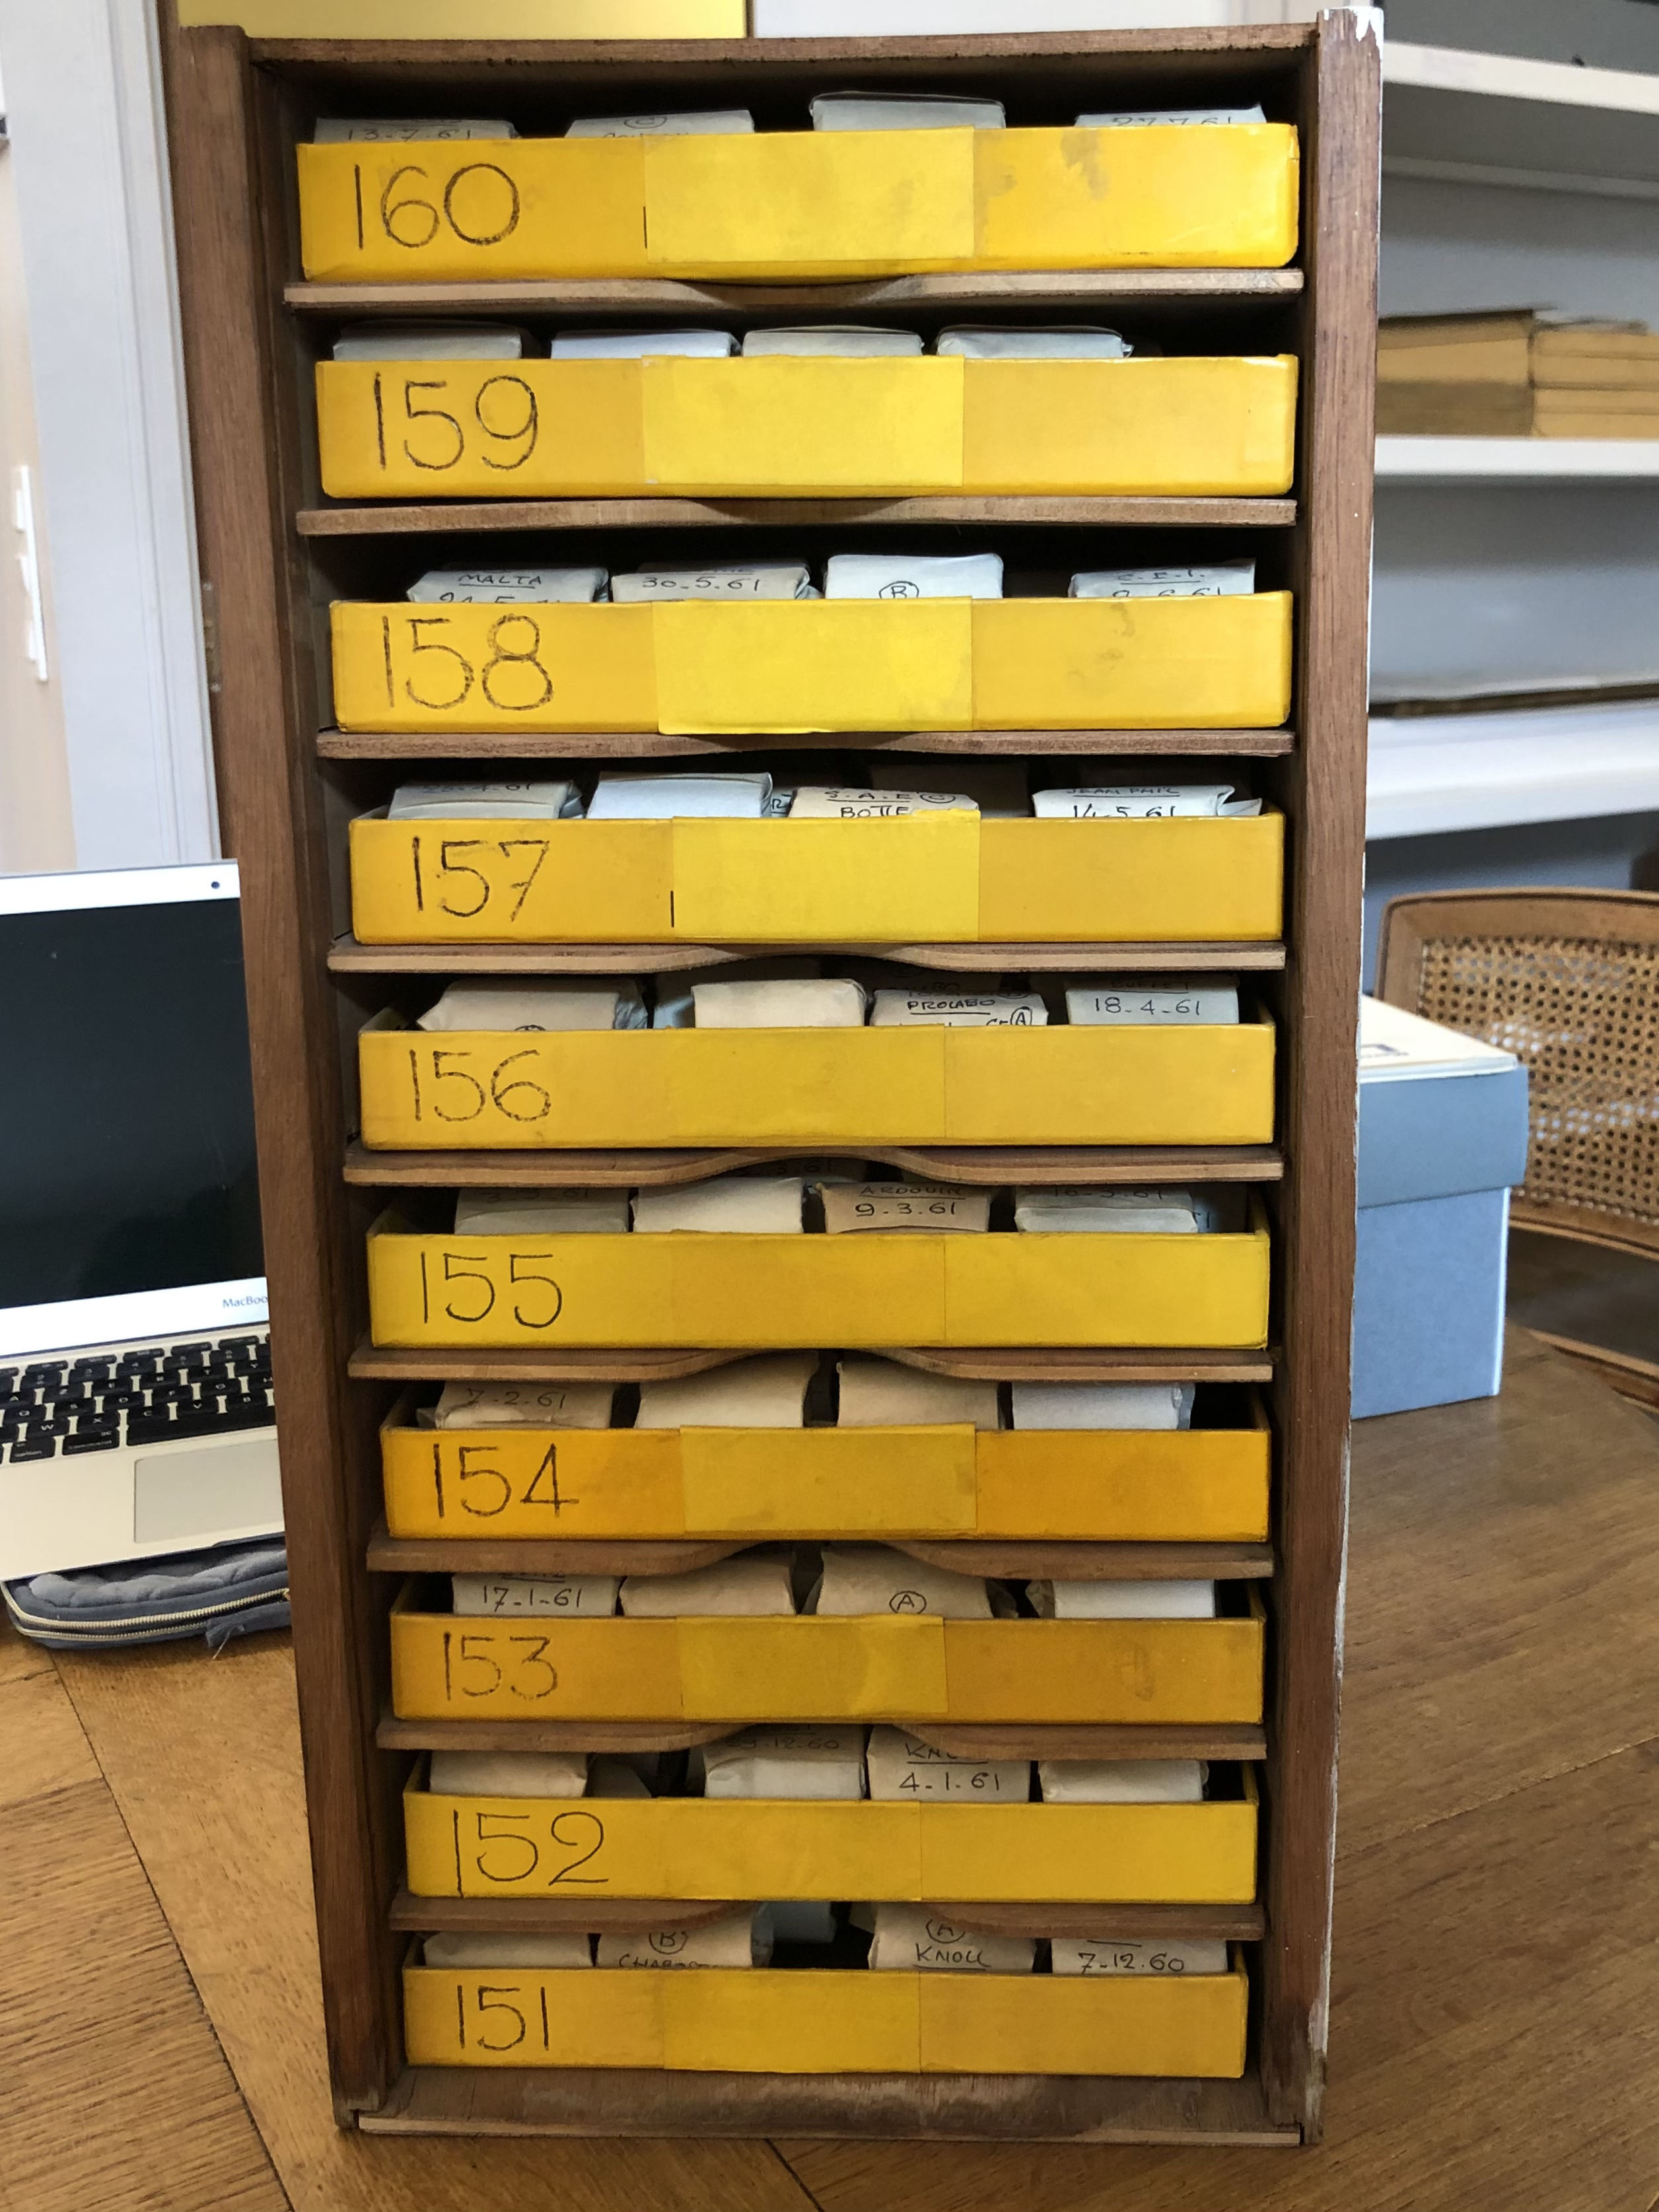
\includegraphics[width=0.75\linewidth]{Illustrations/tiroirs.jpg}
    \caption{Photo des tiroirs de pellicules numérisées}
    \label{fig:tiroirs}
\end{figure}

\begin{figure}[H]
    \centering
    \begin{subfigure}{0.24\textwidth}
        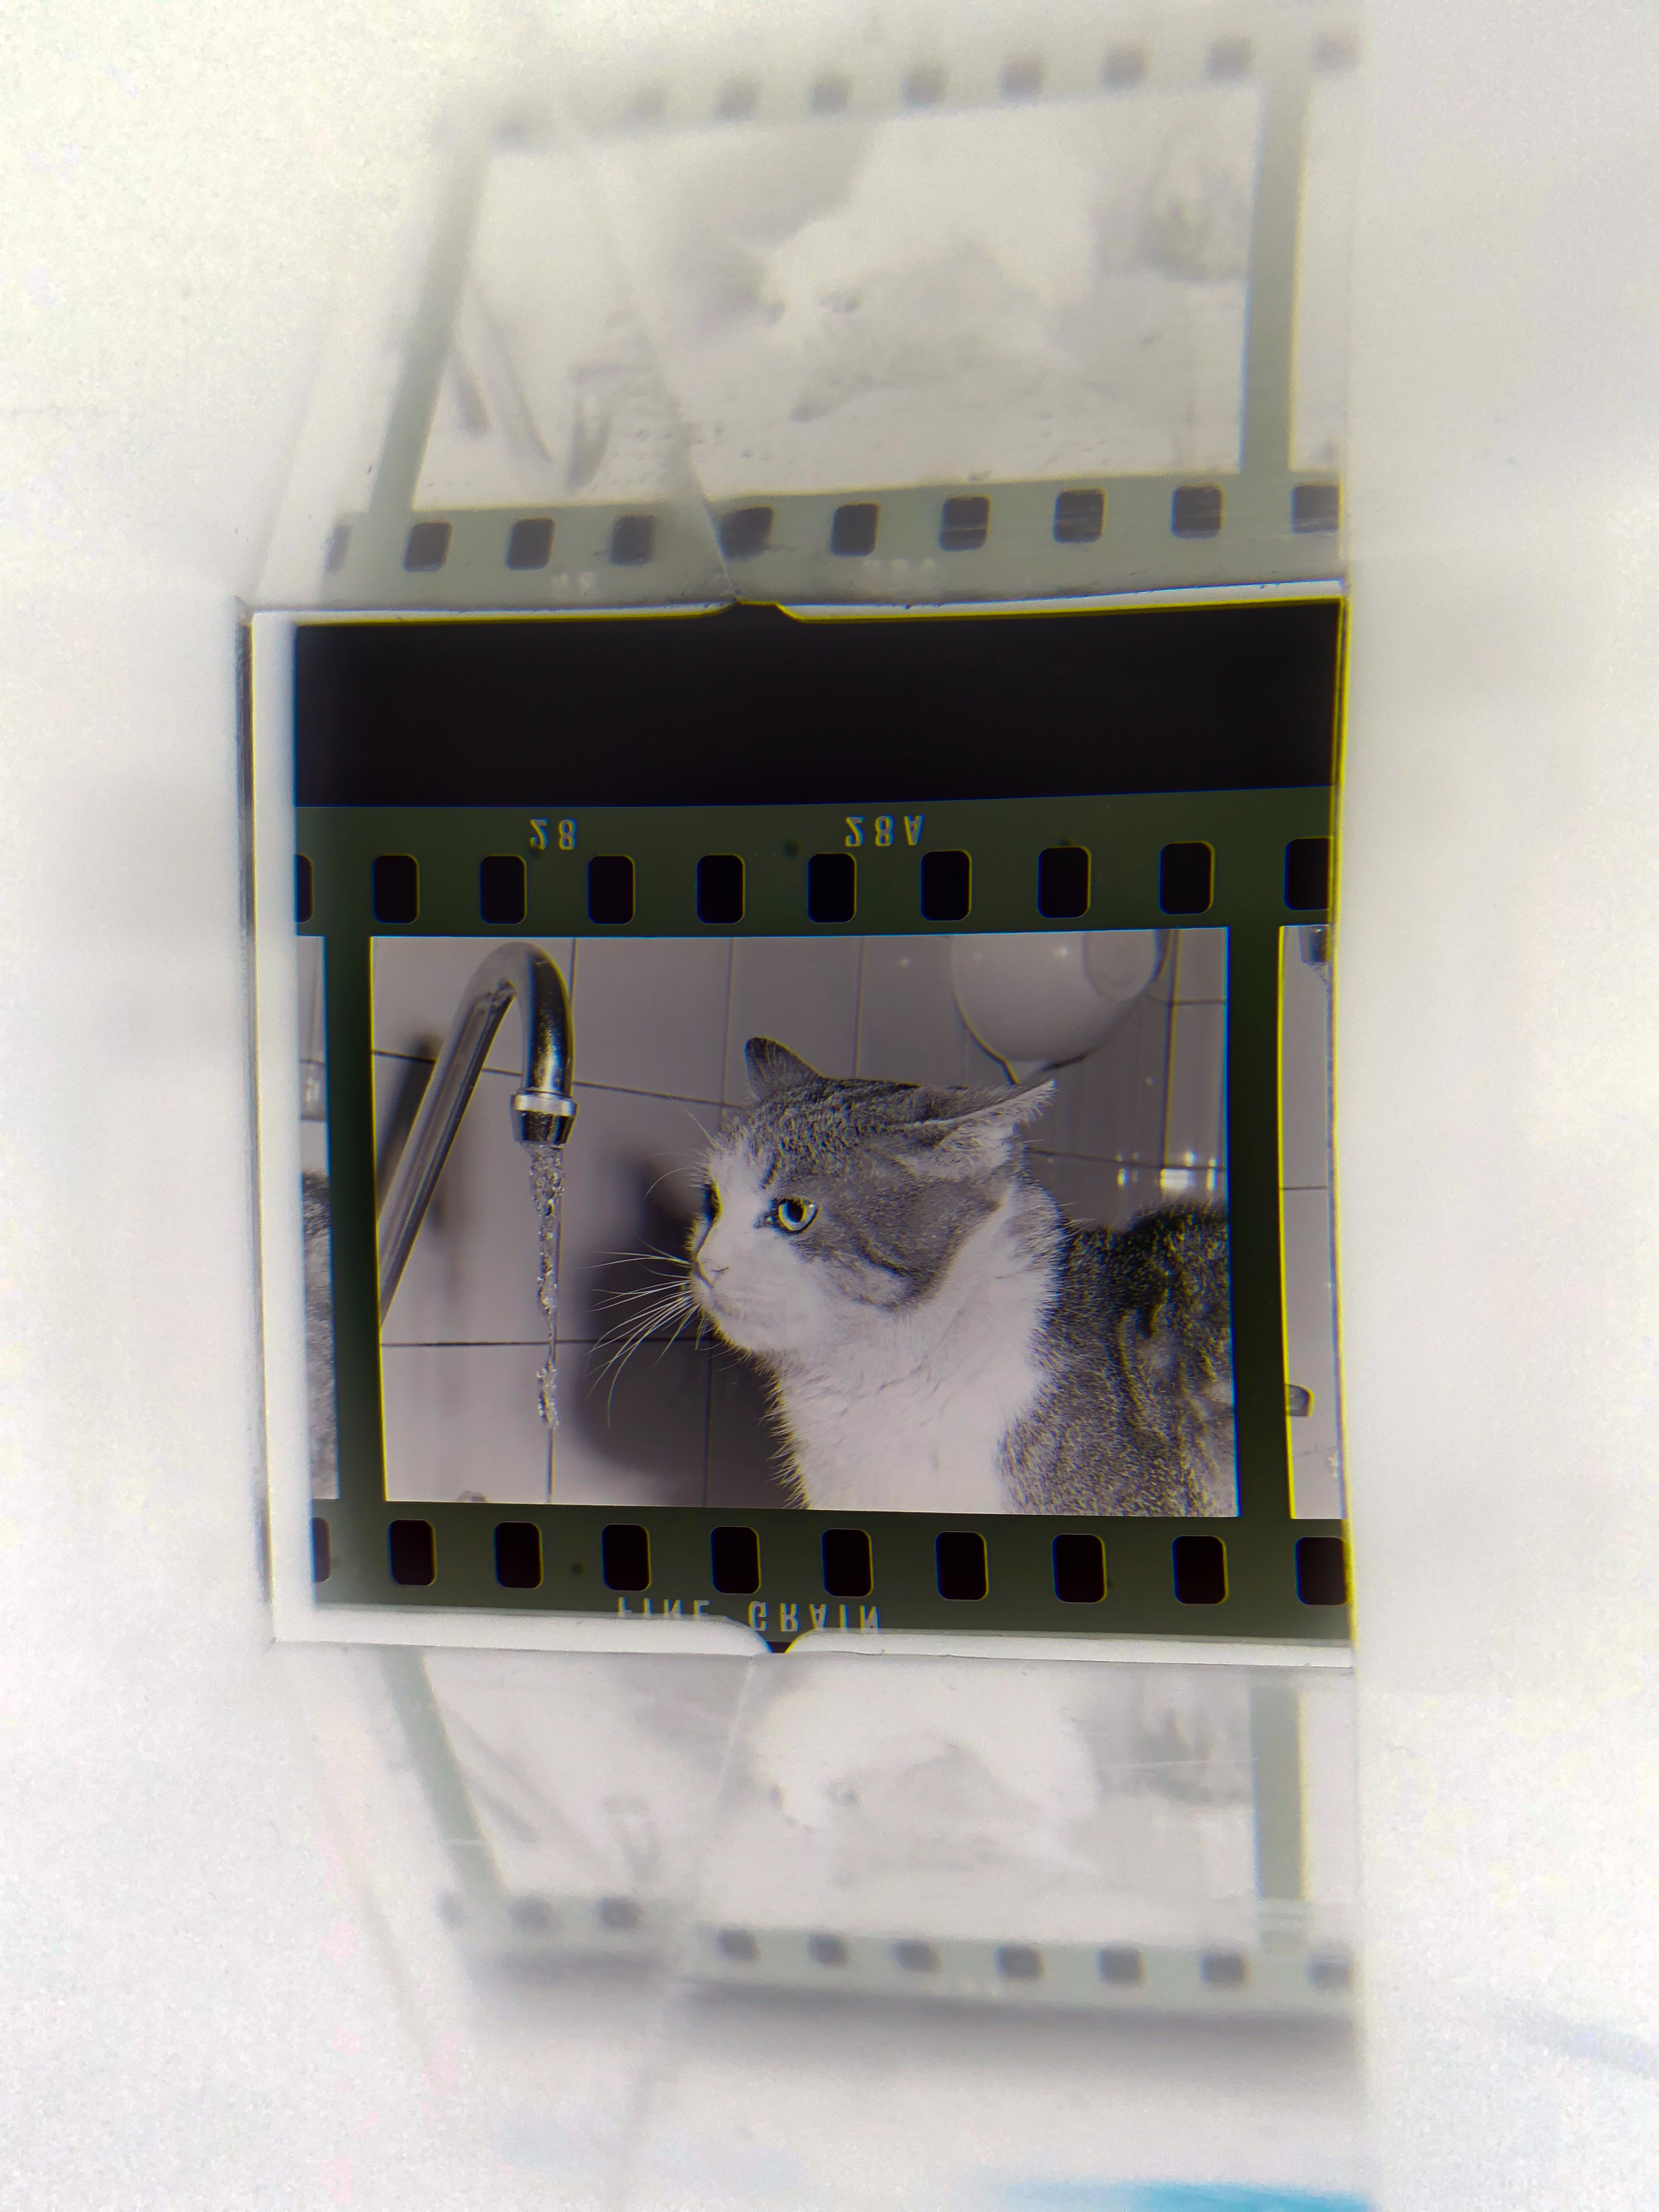
\includegraphics[width=\linewidth]{Illustrations/P1.jpg}
        \caption{}
    \end{subfigure}
    \begin{subfigure}{0.24\textwidth}
        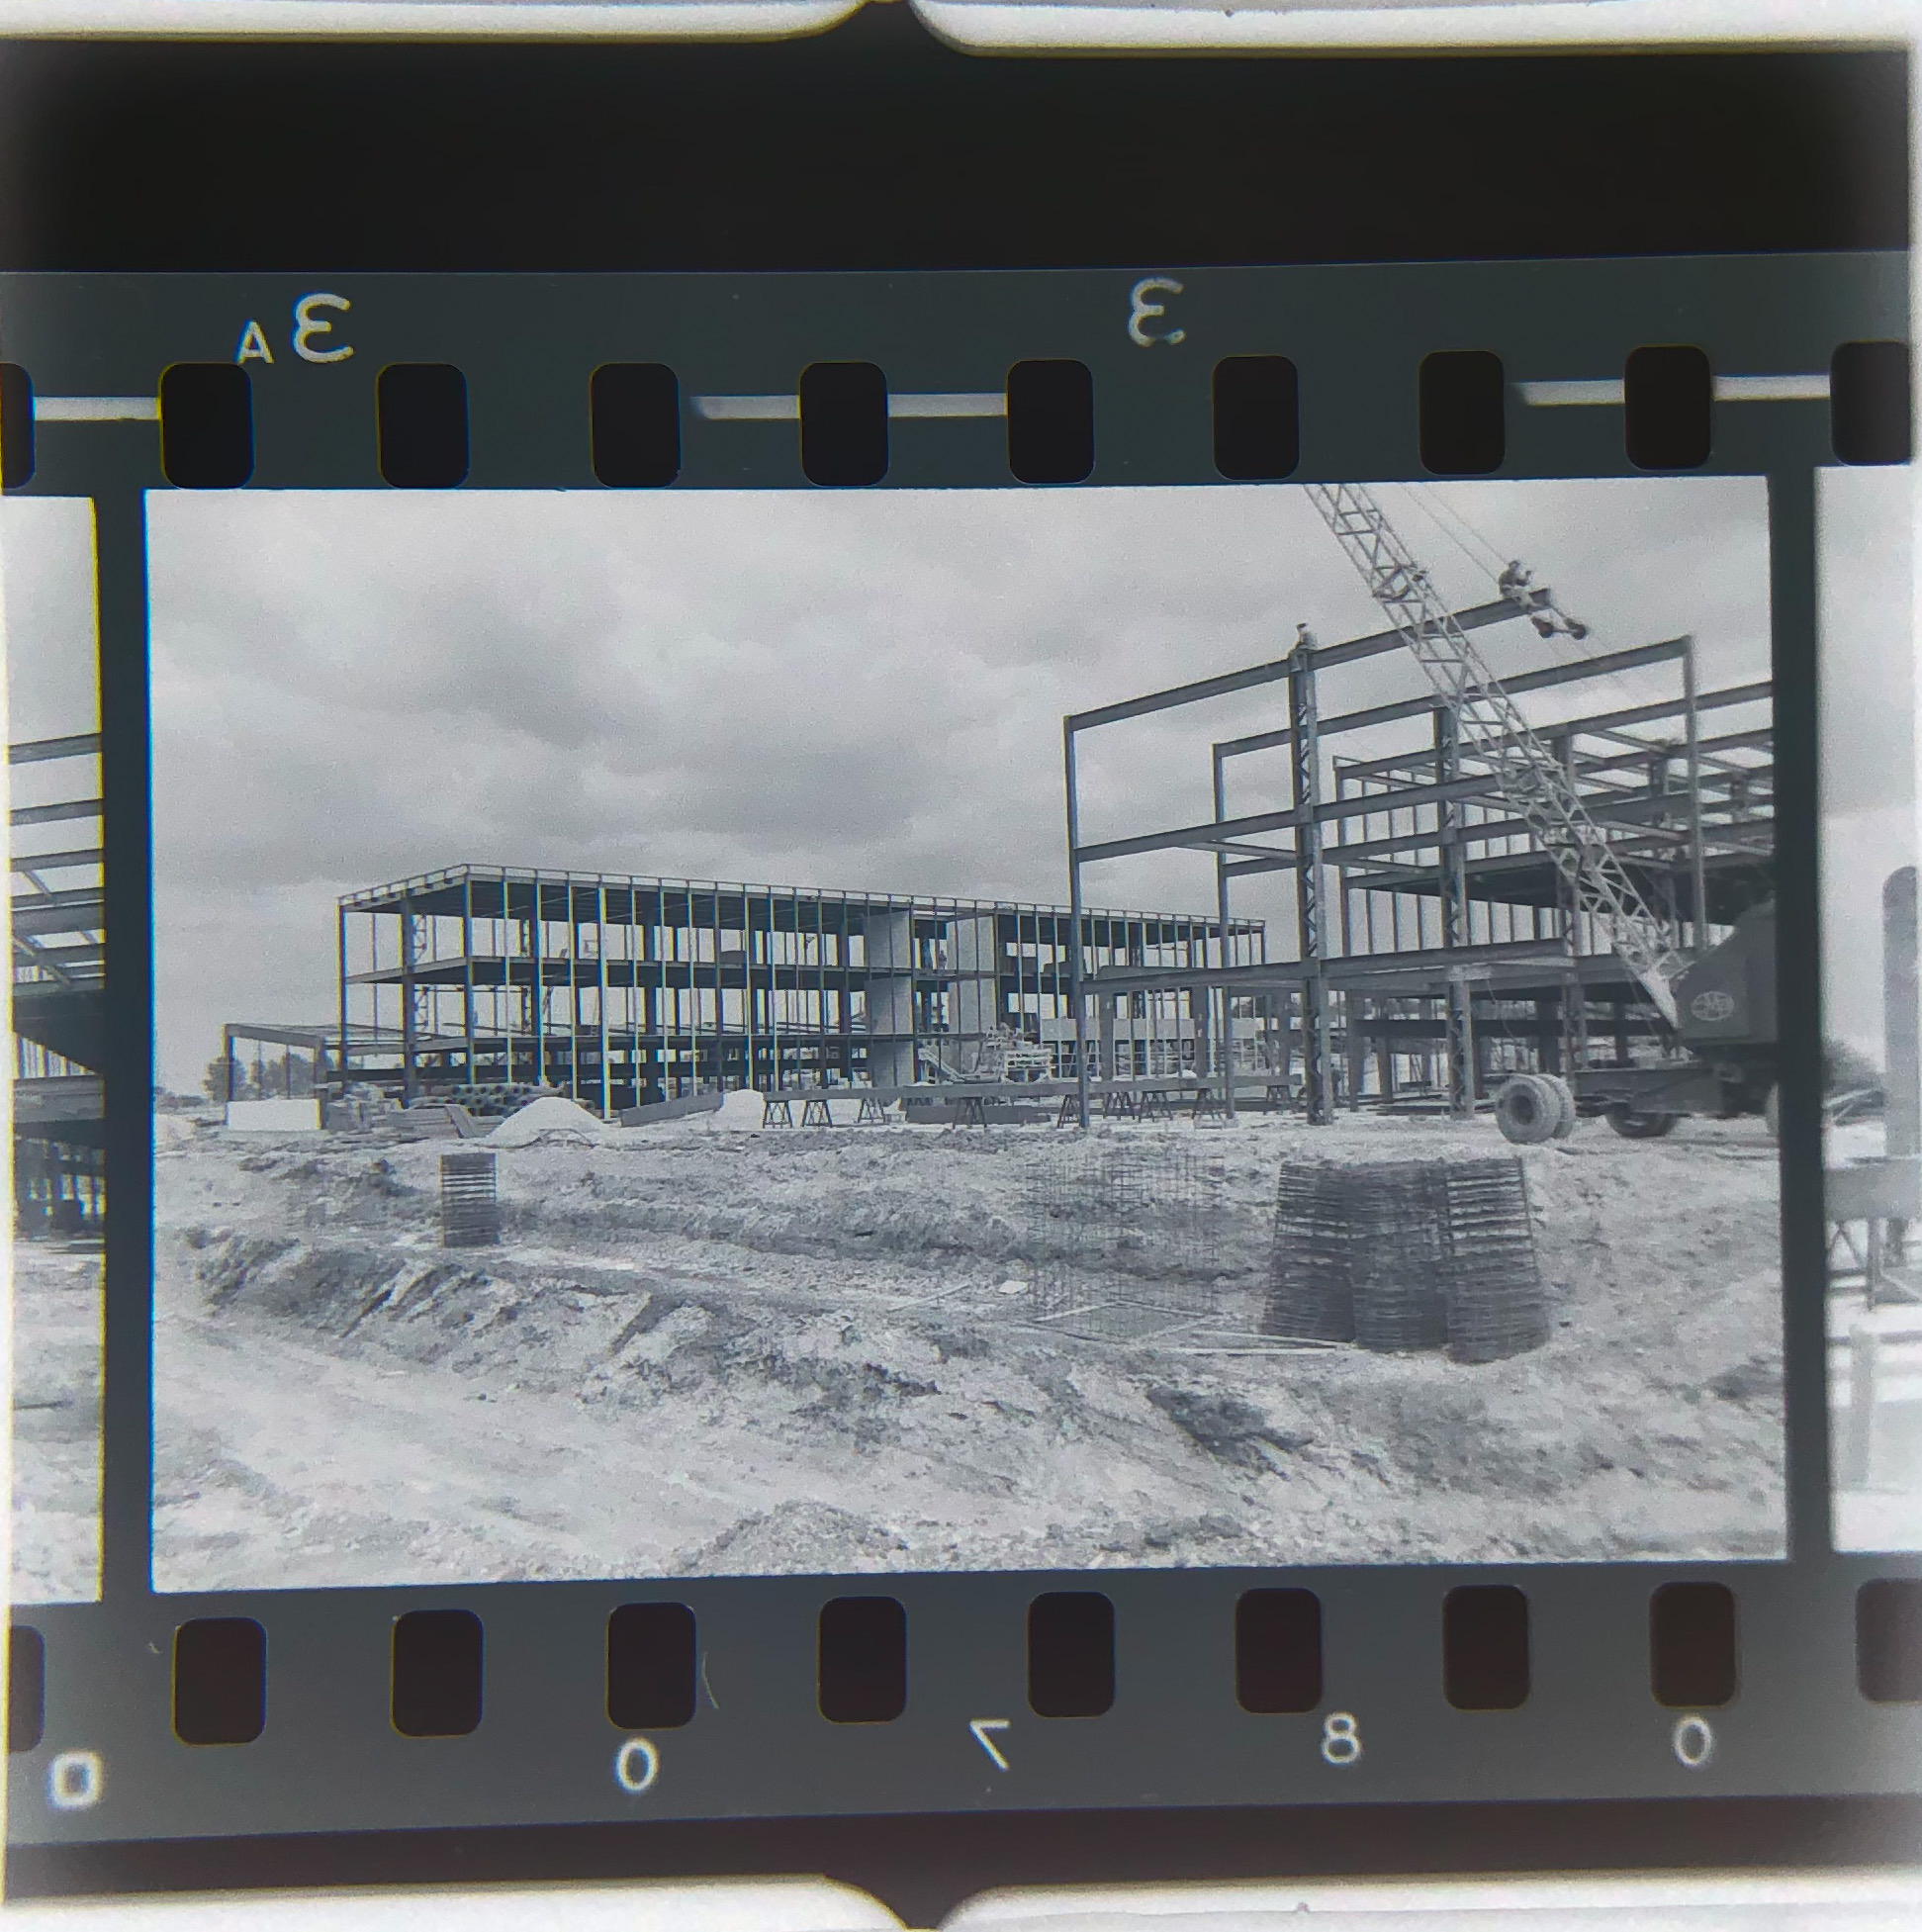
\includegraphics[width=\linewidth]{Illustrations/P2.jpg}
        \caption{}
    \end{subfigure}
    \begin{subfigure}{0.24\textwidth}
        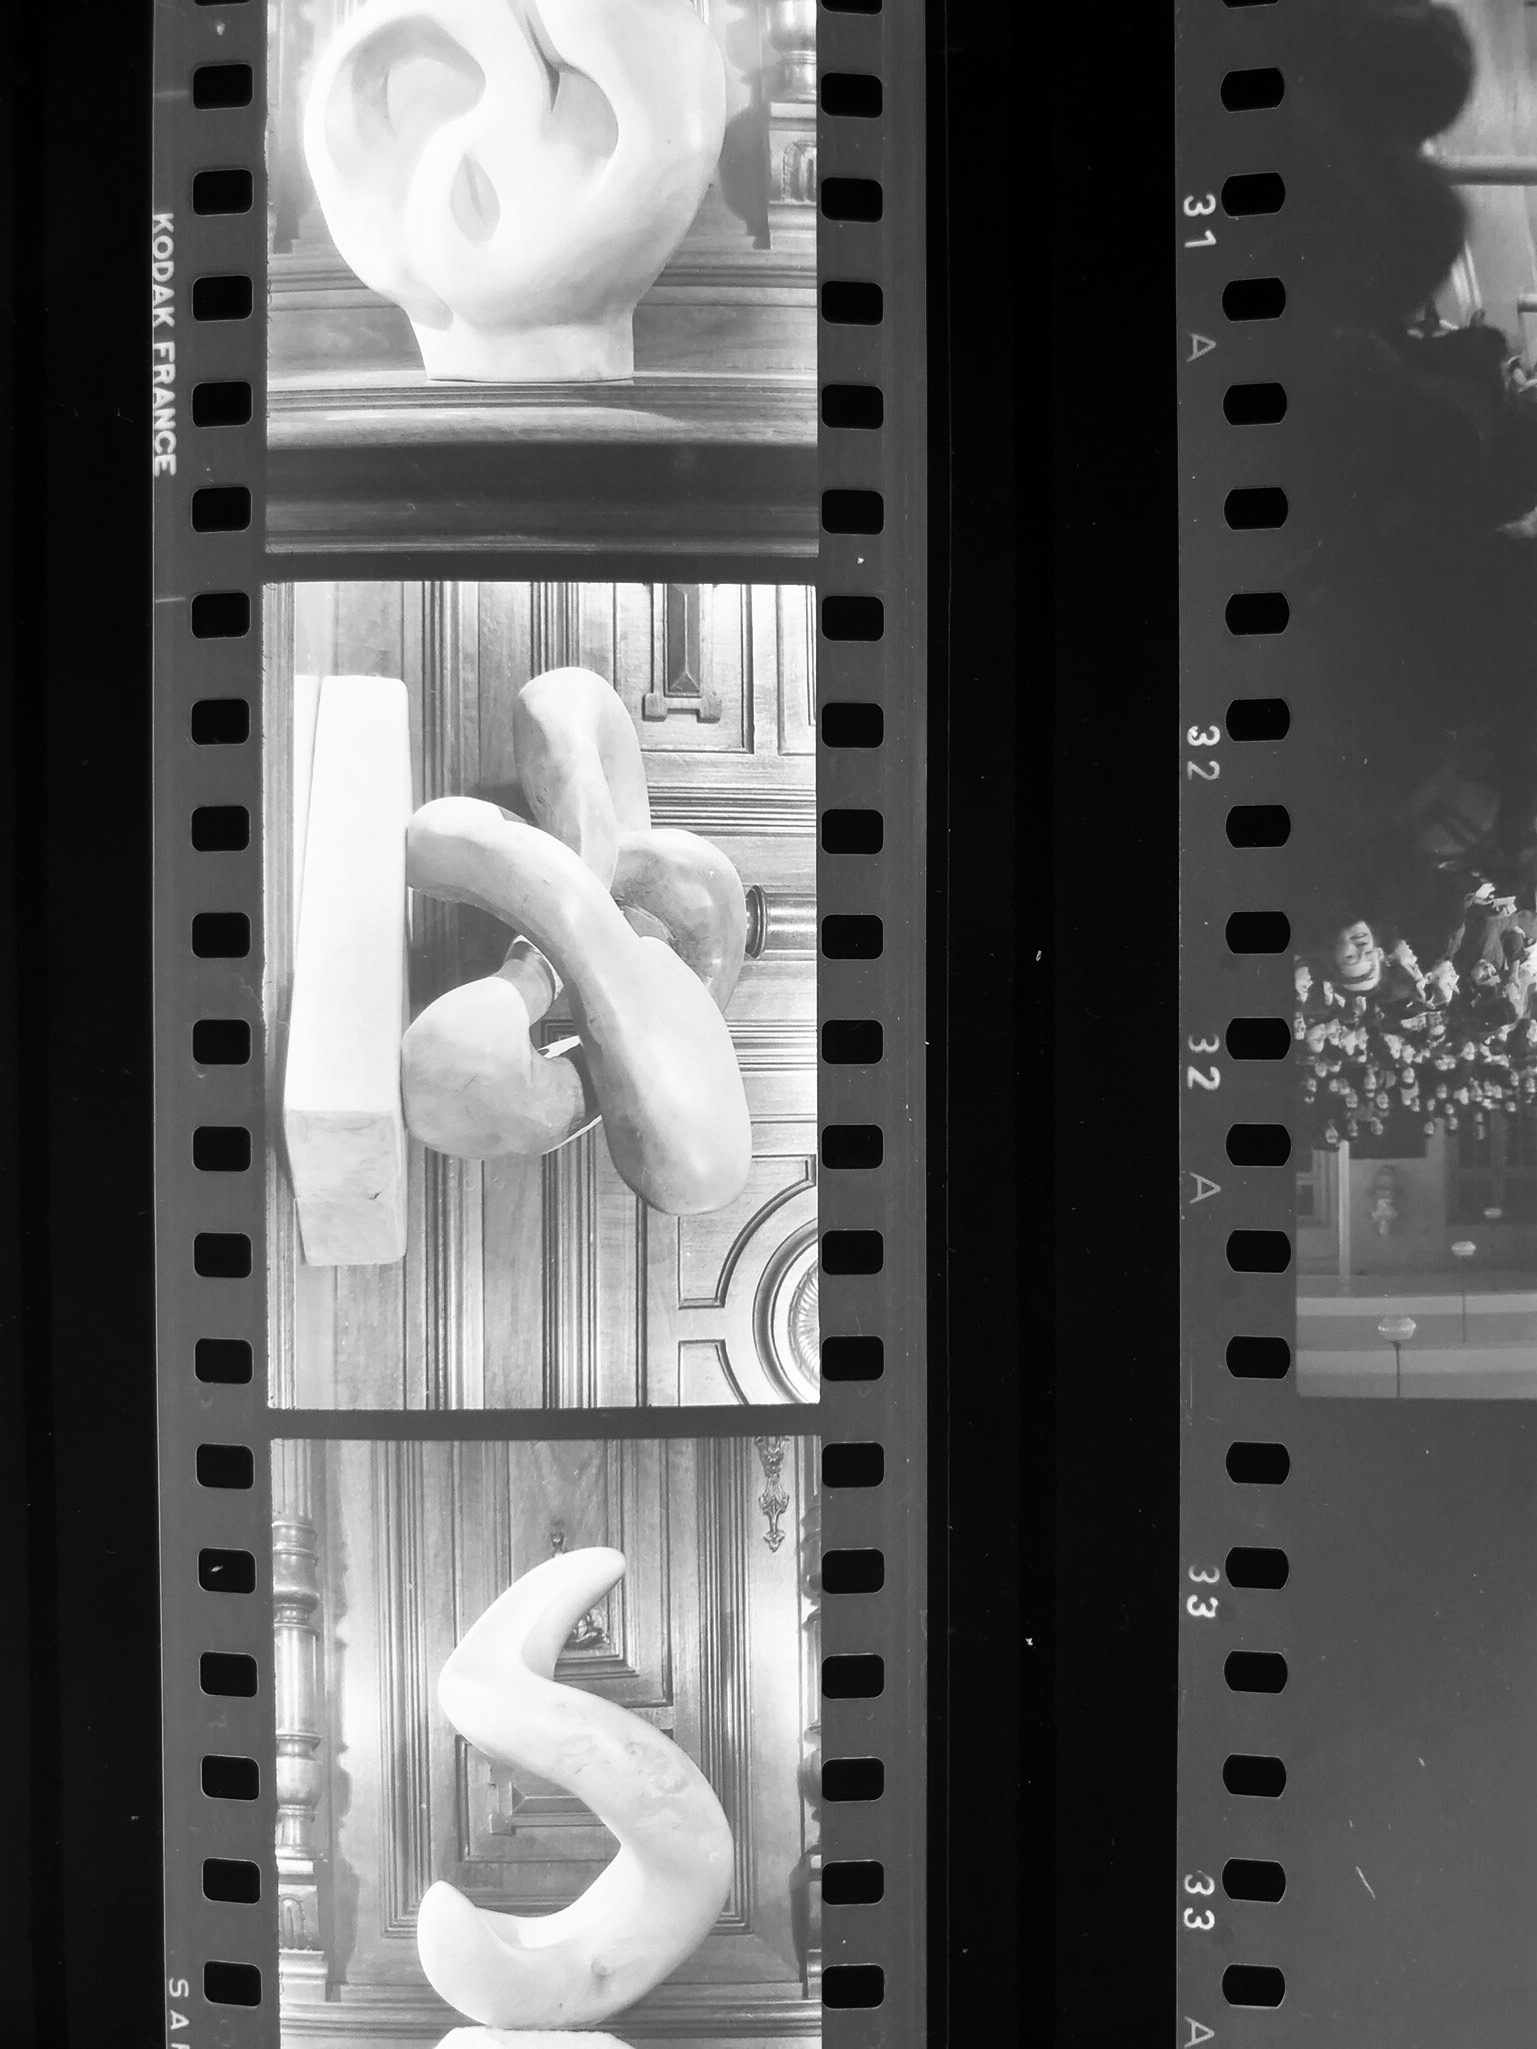
\includegraphics[width=\linewidth]{Illustrations/P3.jpg}
        \caption{}
    \end{subfigure}
    \begin{subfigure}{0.24\textwidth}
        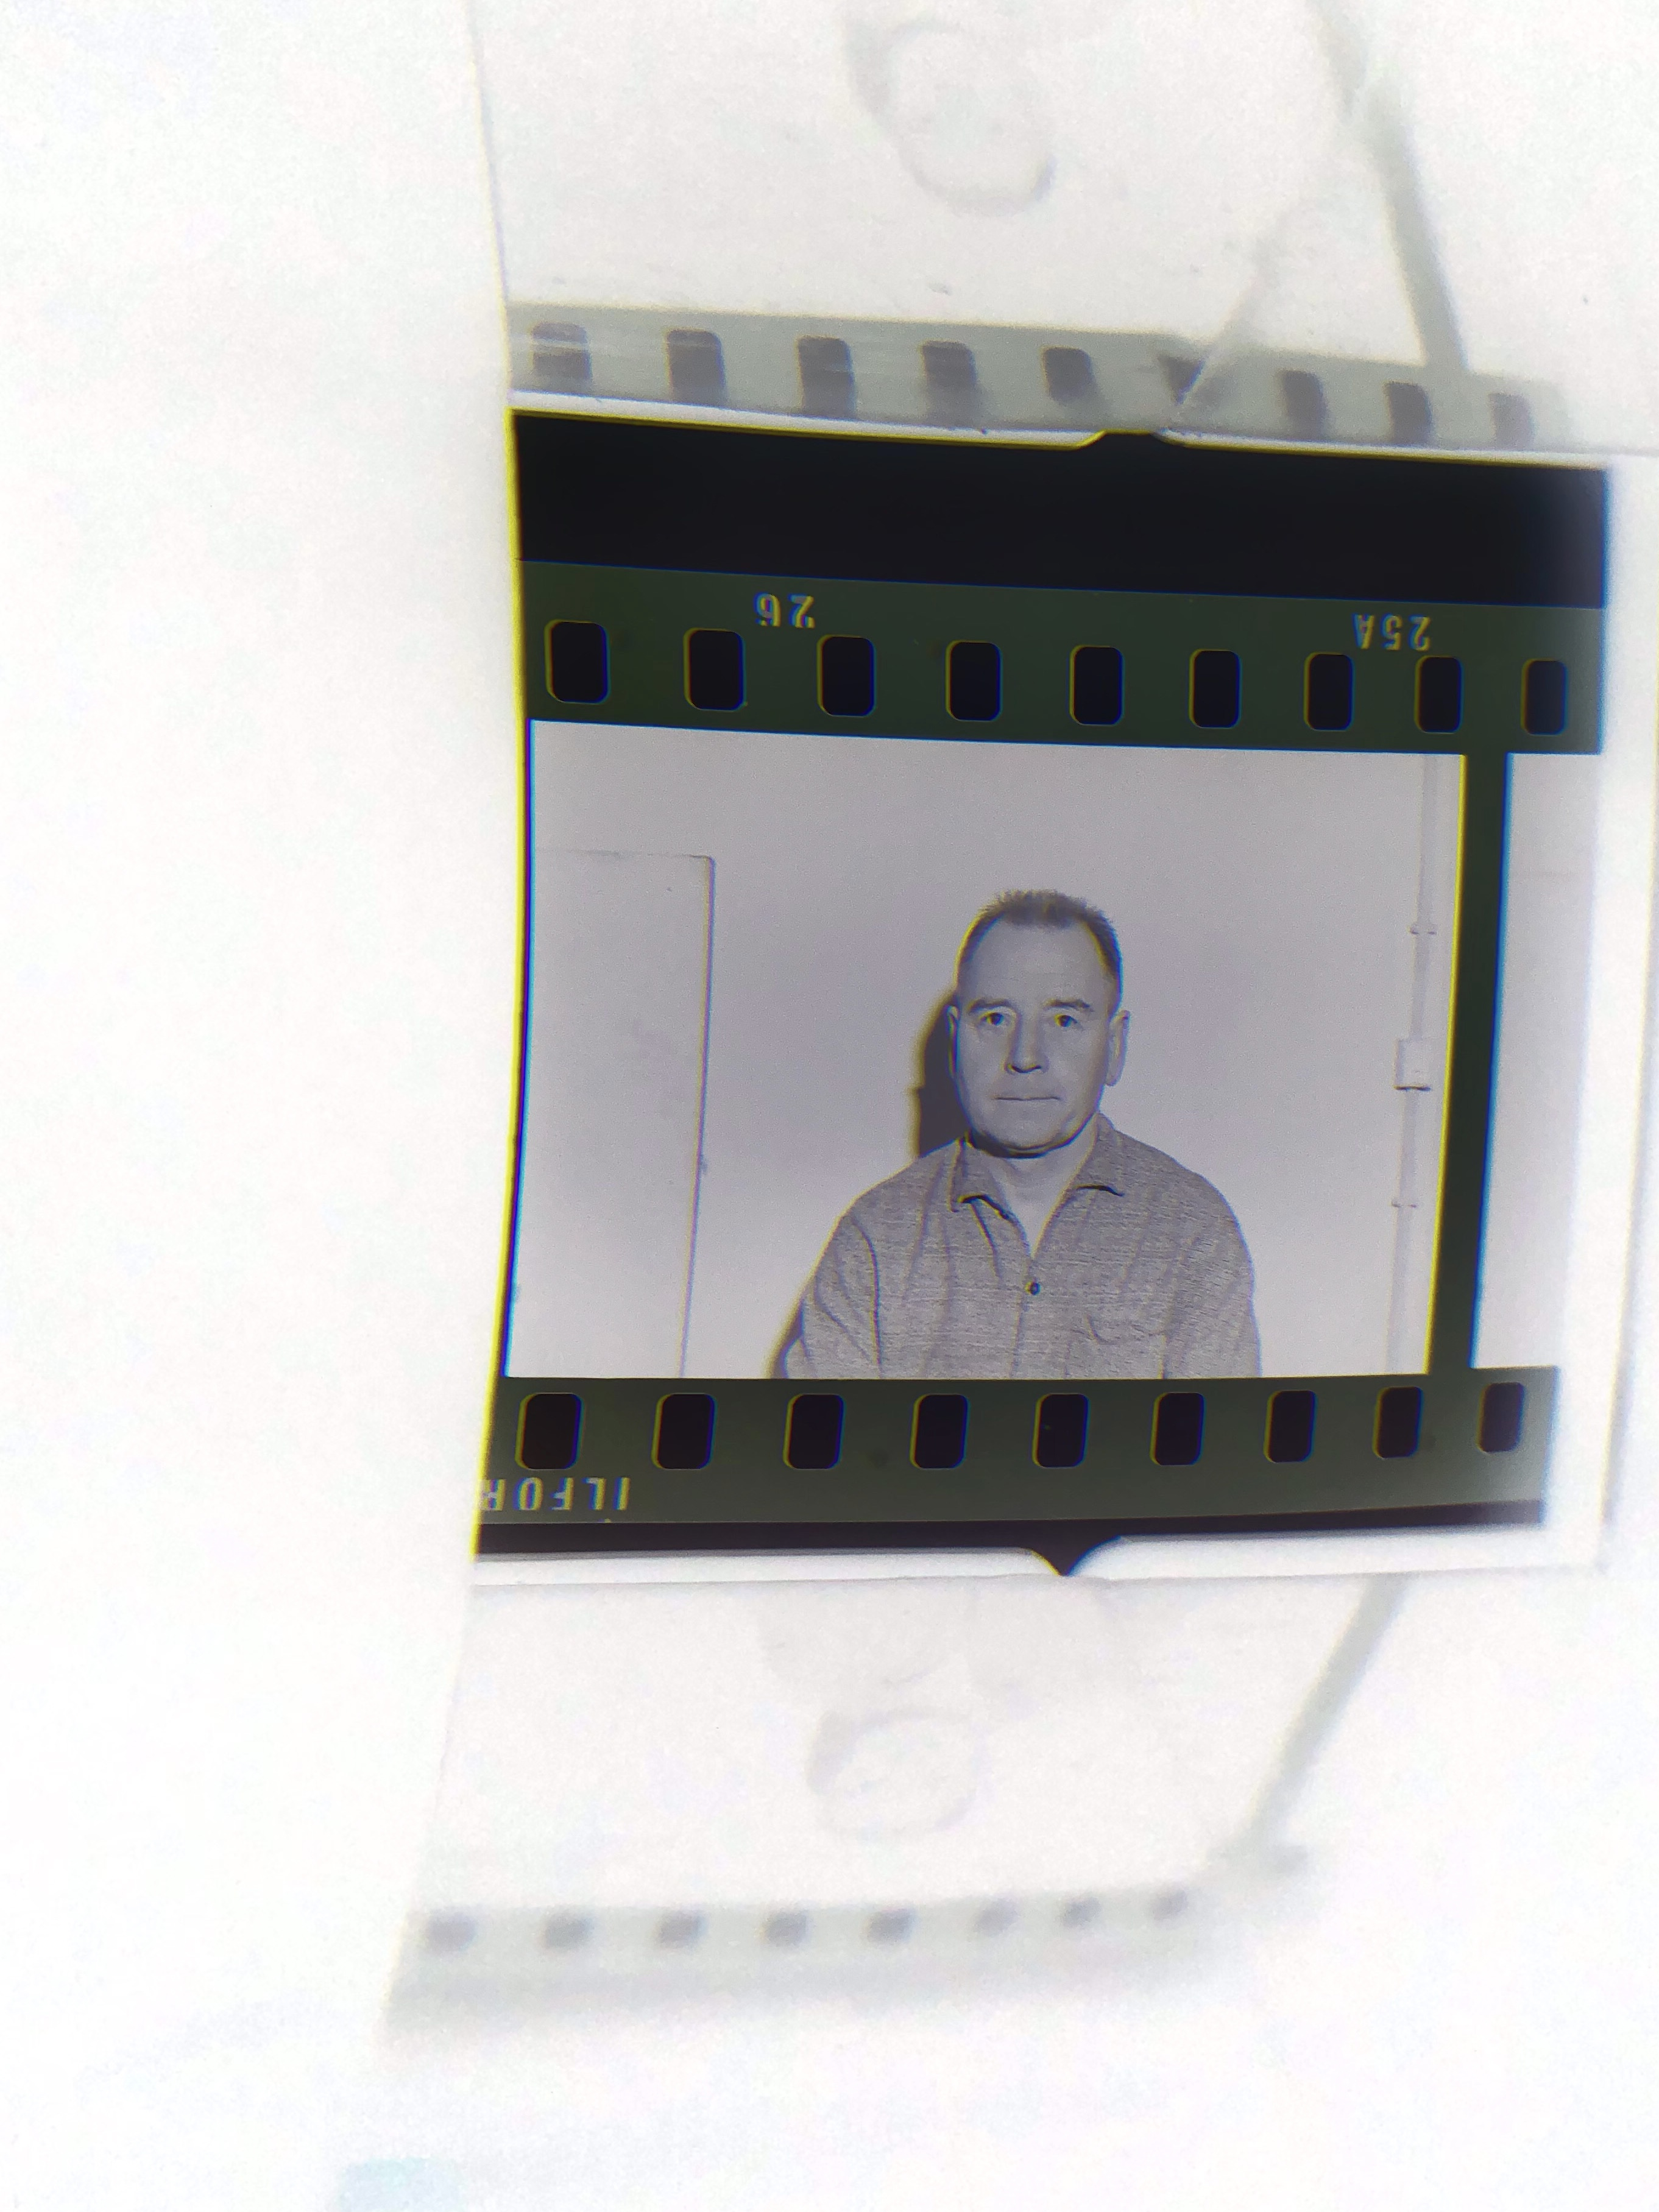
\includegraphics[width=\linewidth]{Illustrations/P4.jpg}
        \caption{}
    \end{subfigure}
    \begin{subfigure}{0.20\textwidth}
        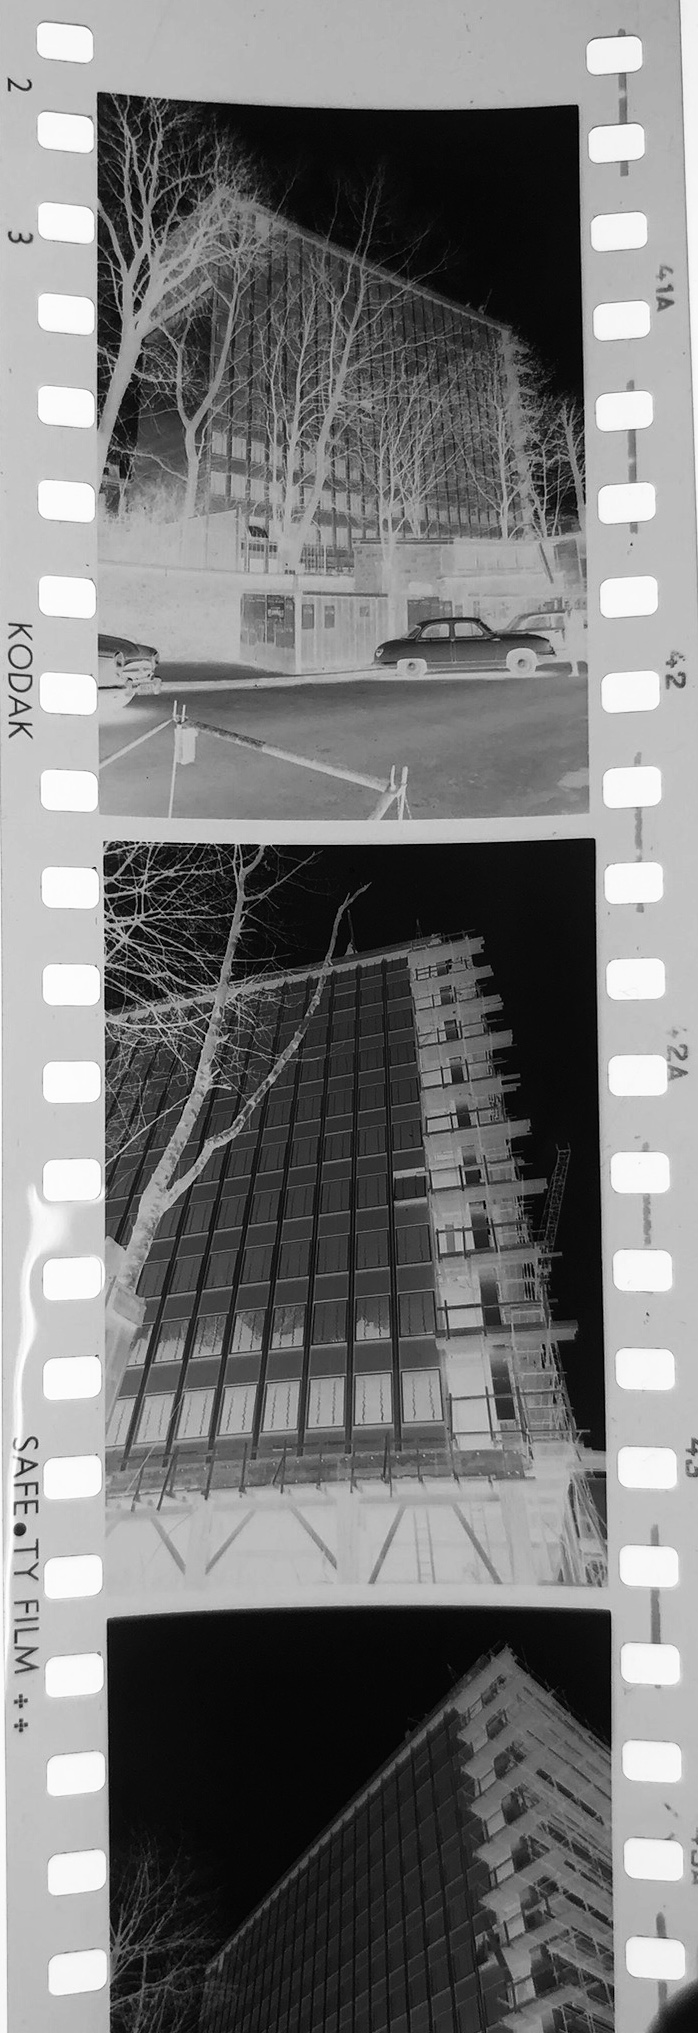
\includegraphics[width=\linewidth]{Illustrations/P5.jpg}
        \caption{}
    \end{subfigure}
    \begin{subfigure}{0.24\textwidth}
        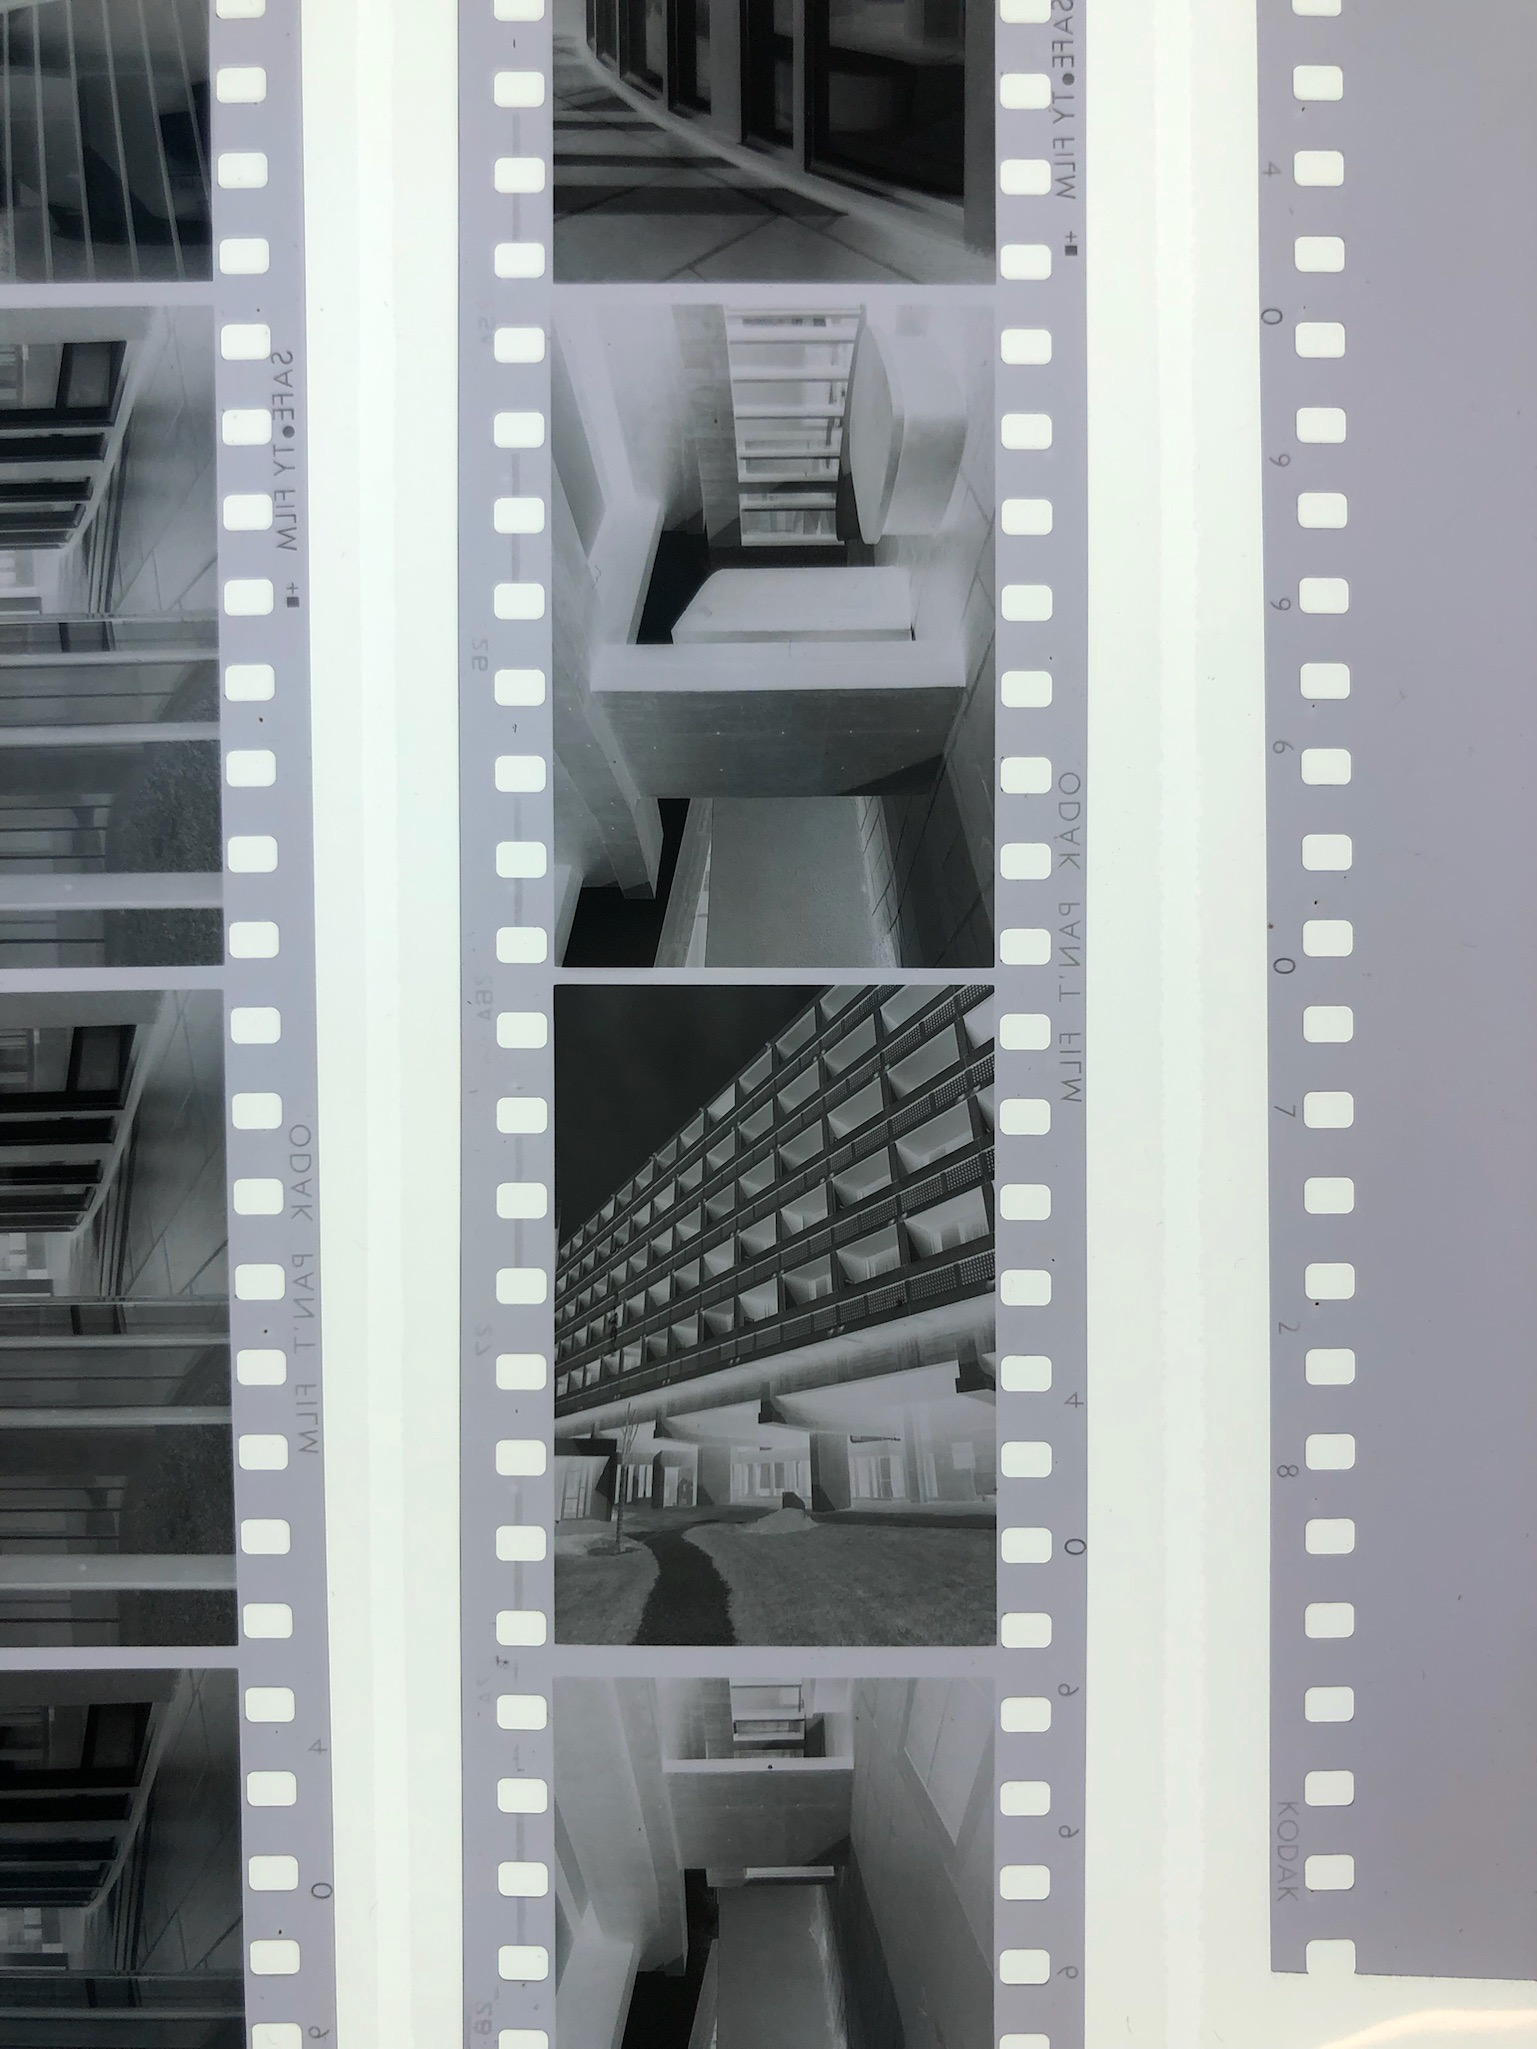
\includegraphics[width=\linewidth]{Illustrations/P6.jpg}
        \caption{}
    \end{subfigure}
    \begin{subfigure}{0.24\textwidth}
        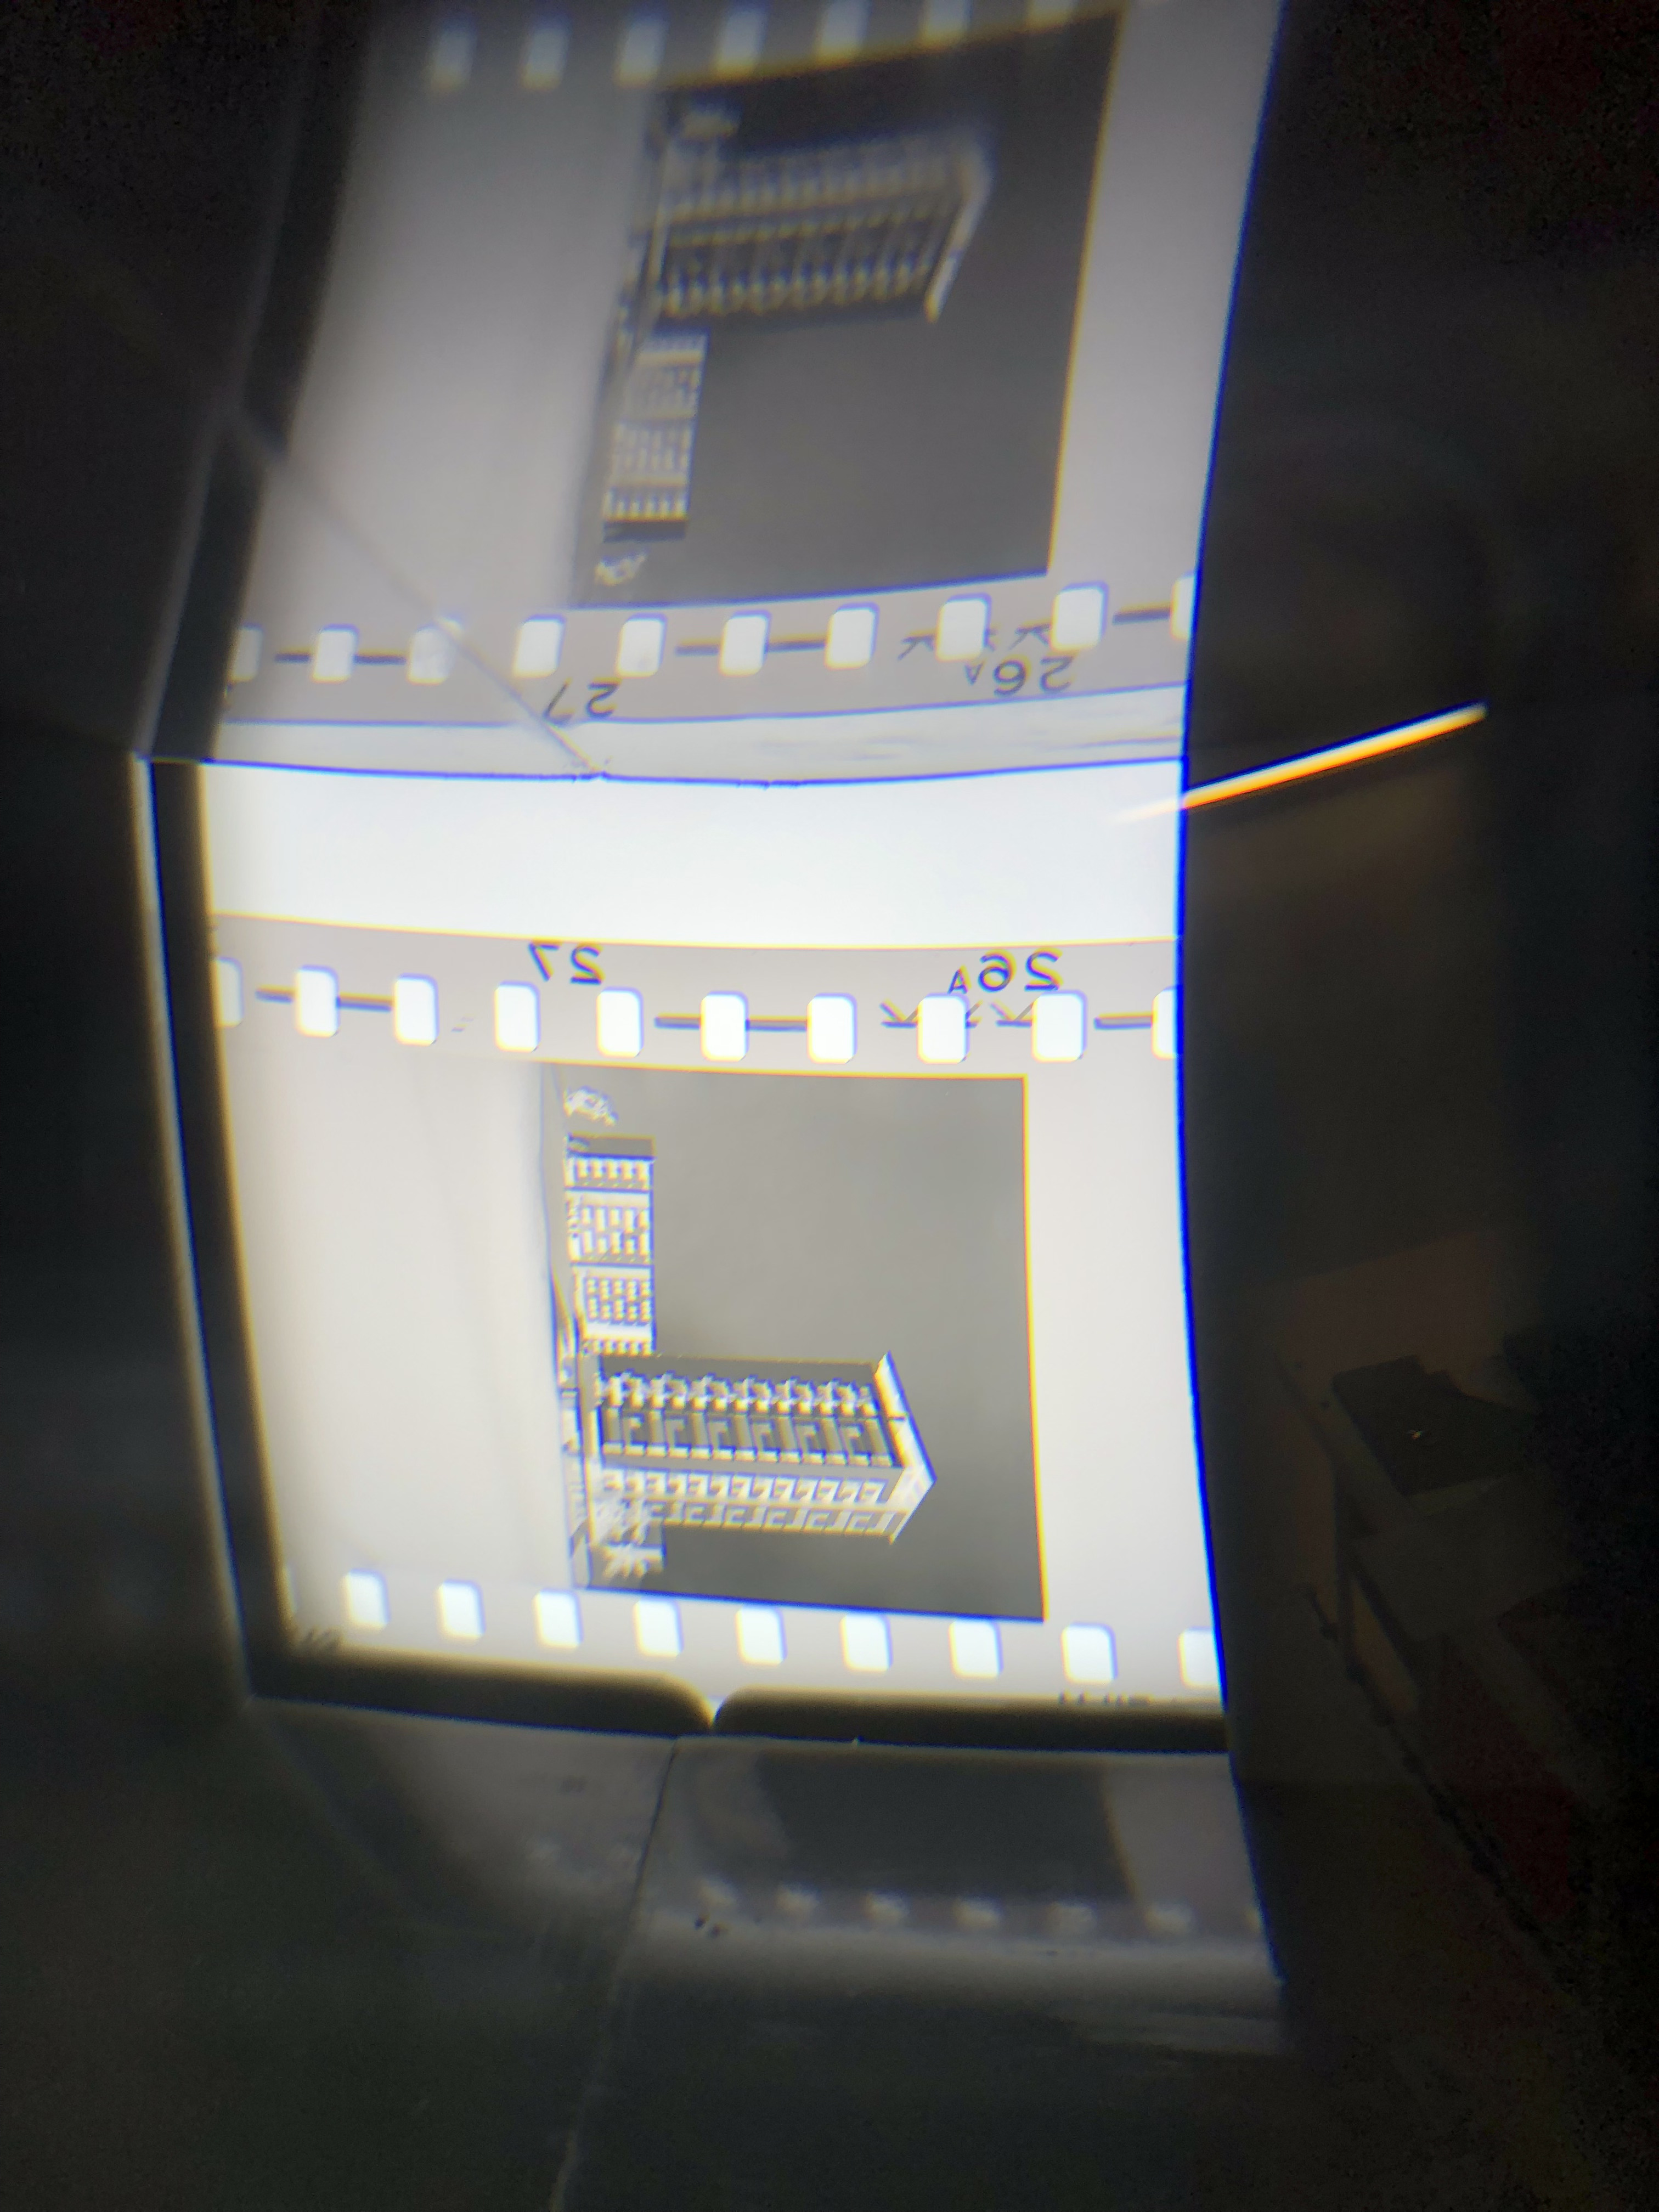
\includegraphics[width=\linewidth]{Illustrations/P7.jpg}
        \caption{}
    \end{subfigure}
    \begin{subfigure}{0.24\textwidth}
        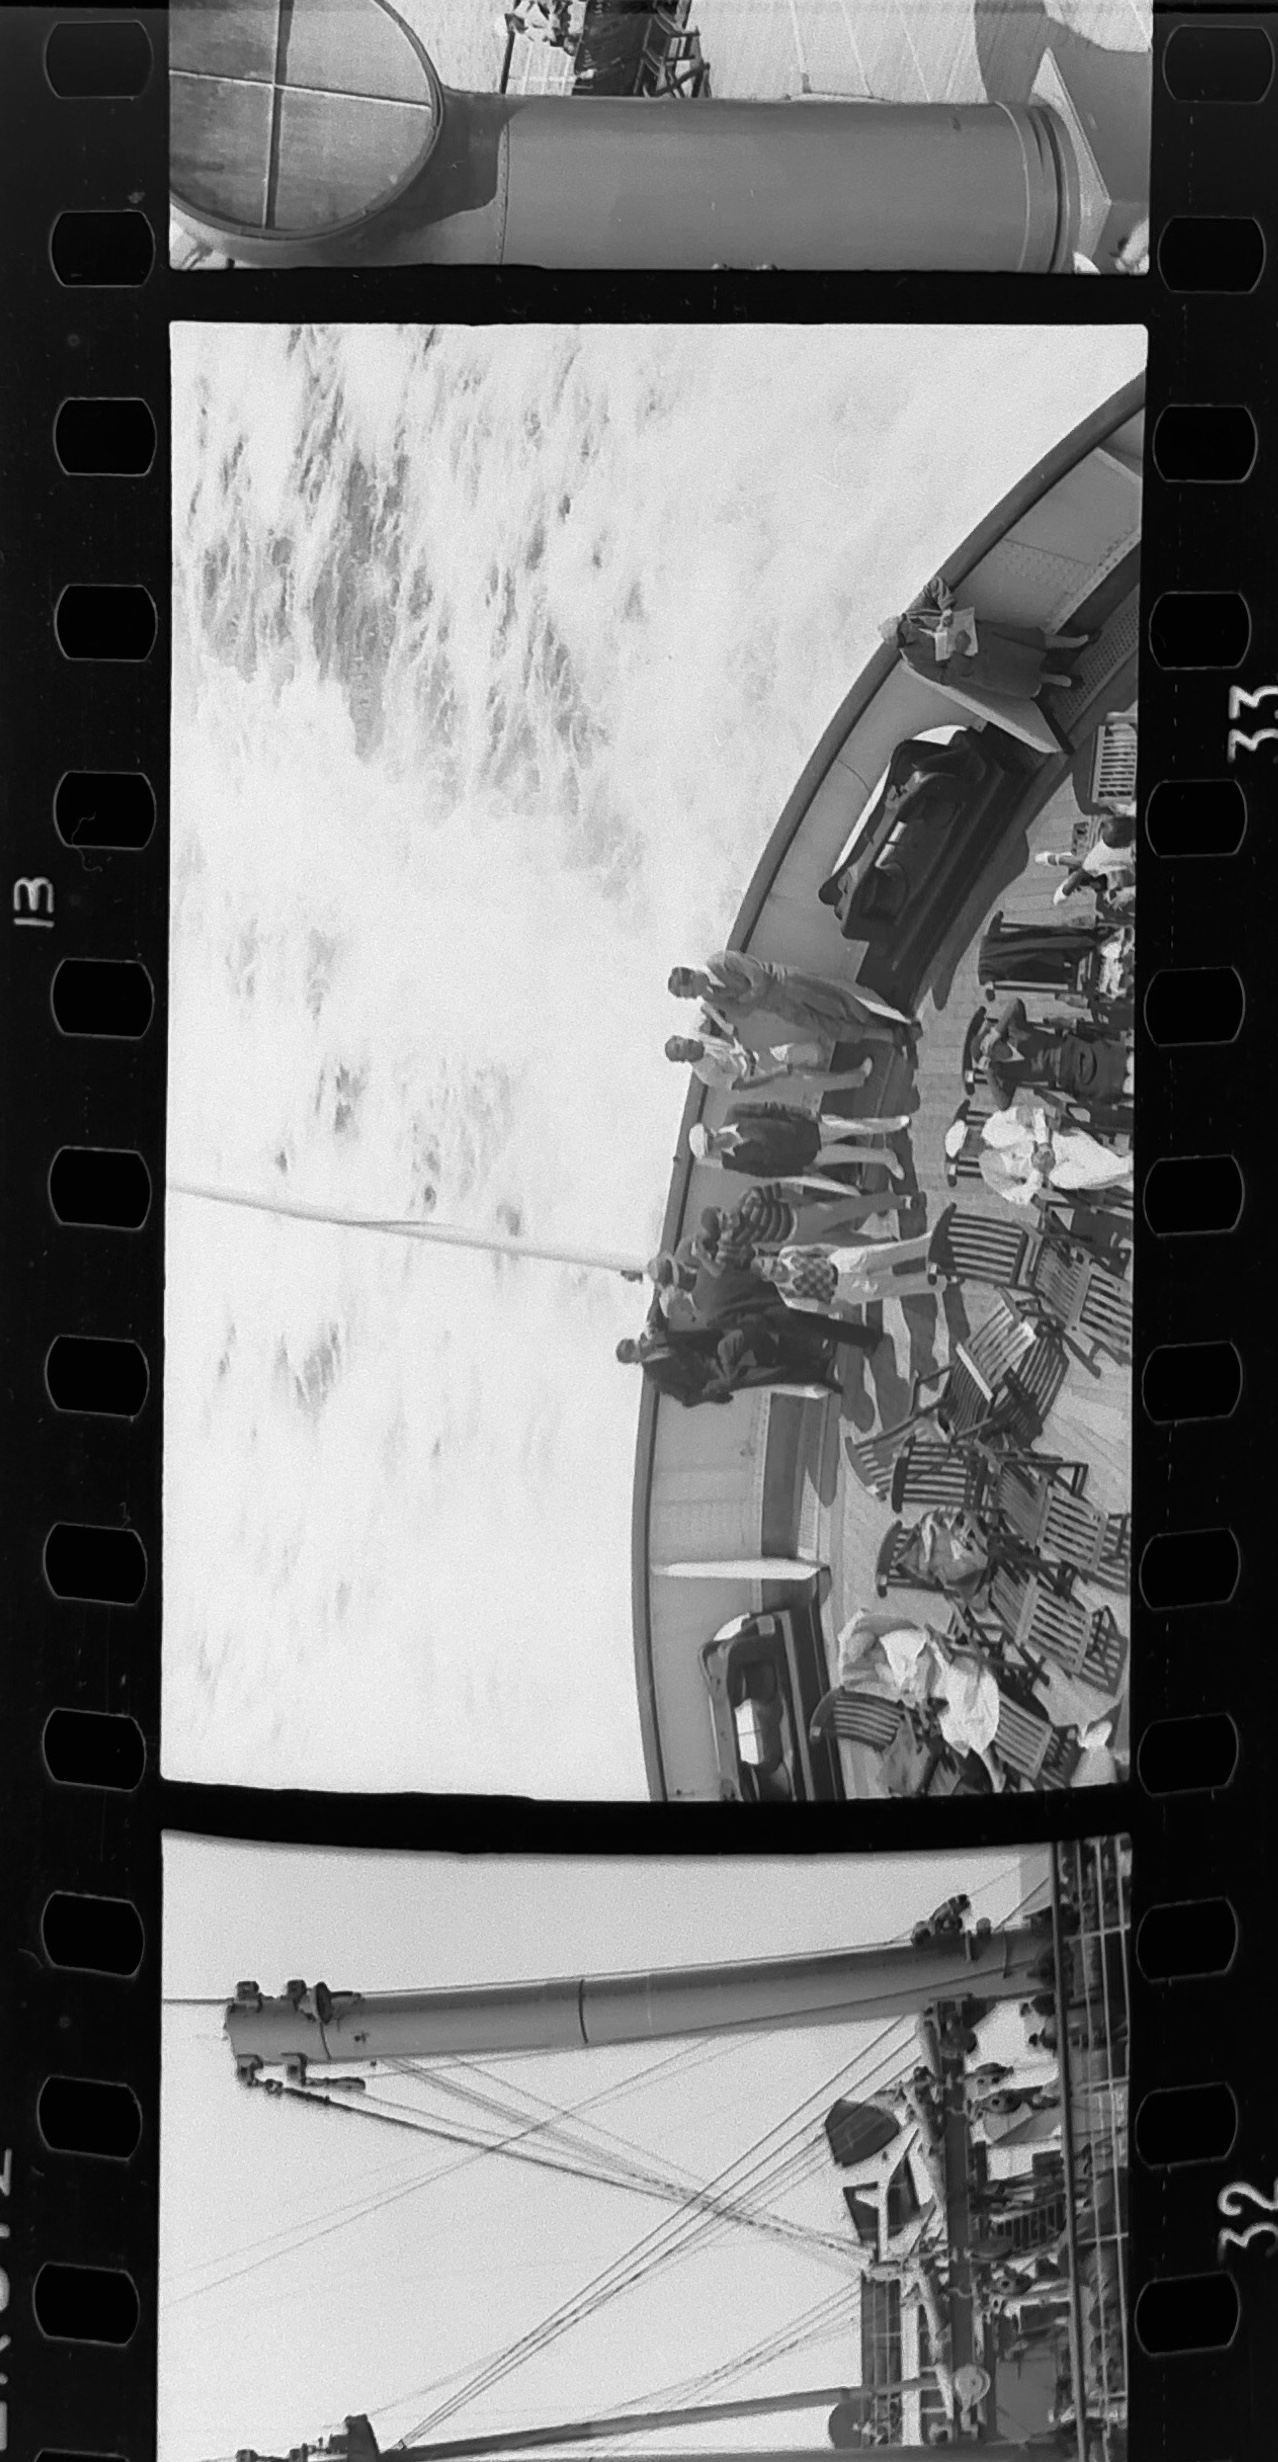
\includegraphics[width=\linewidth]{Illustrations/P8.jpg}
        \caption{}
    \end{subfigure}    \begin{subfigure}{0.24\textwidth}
        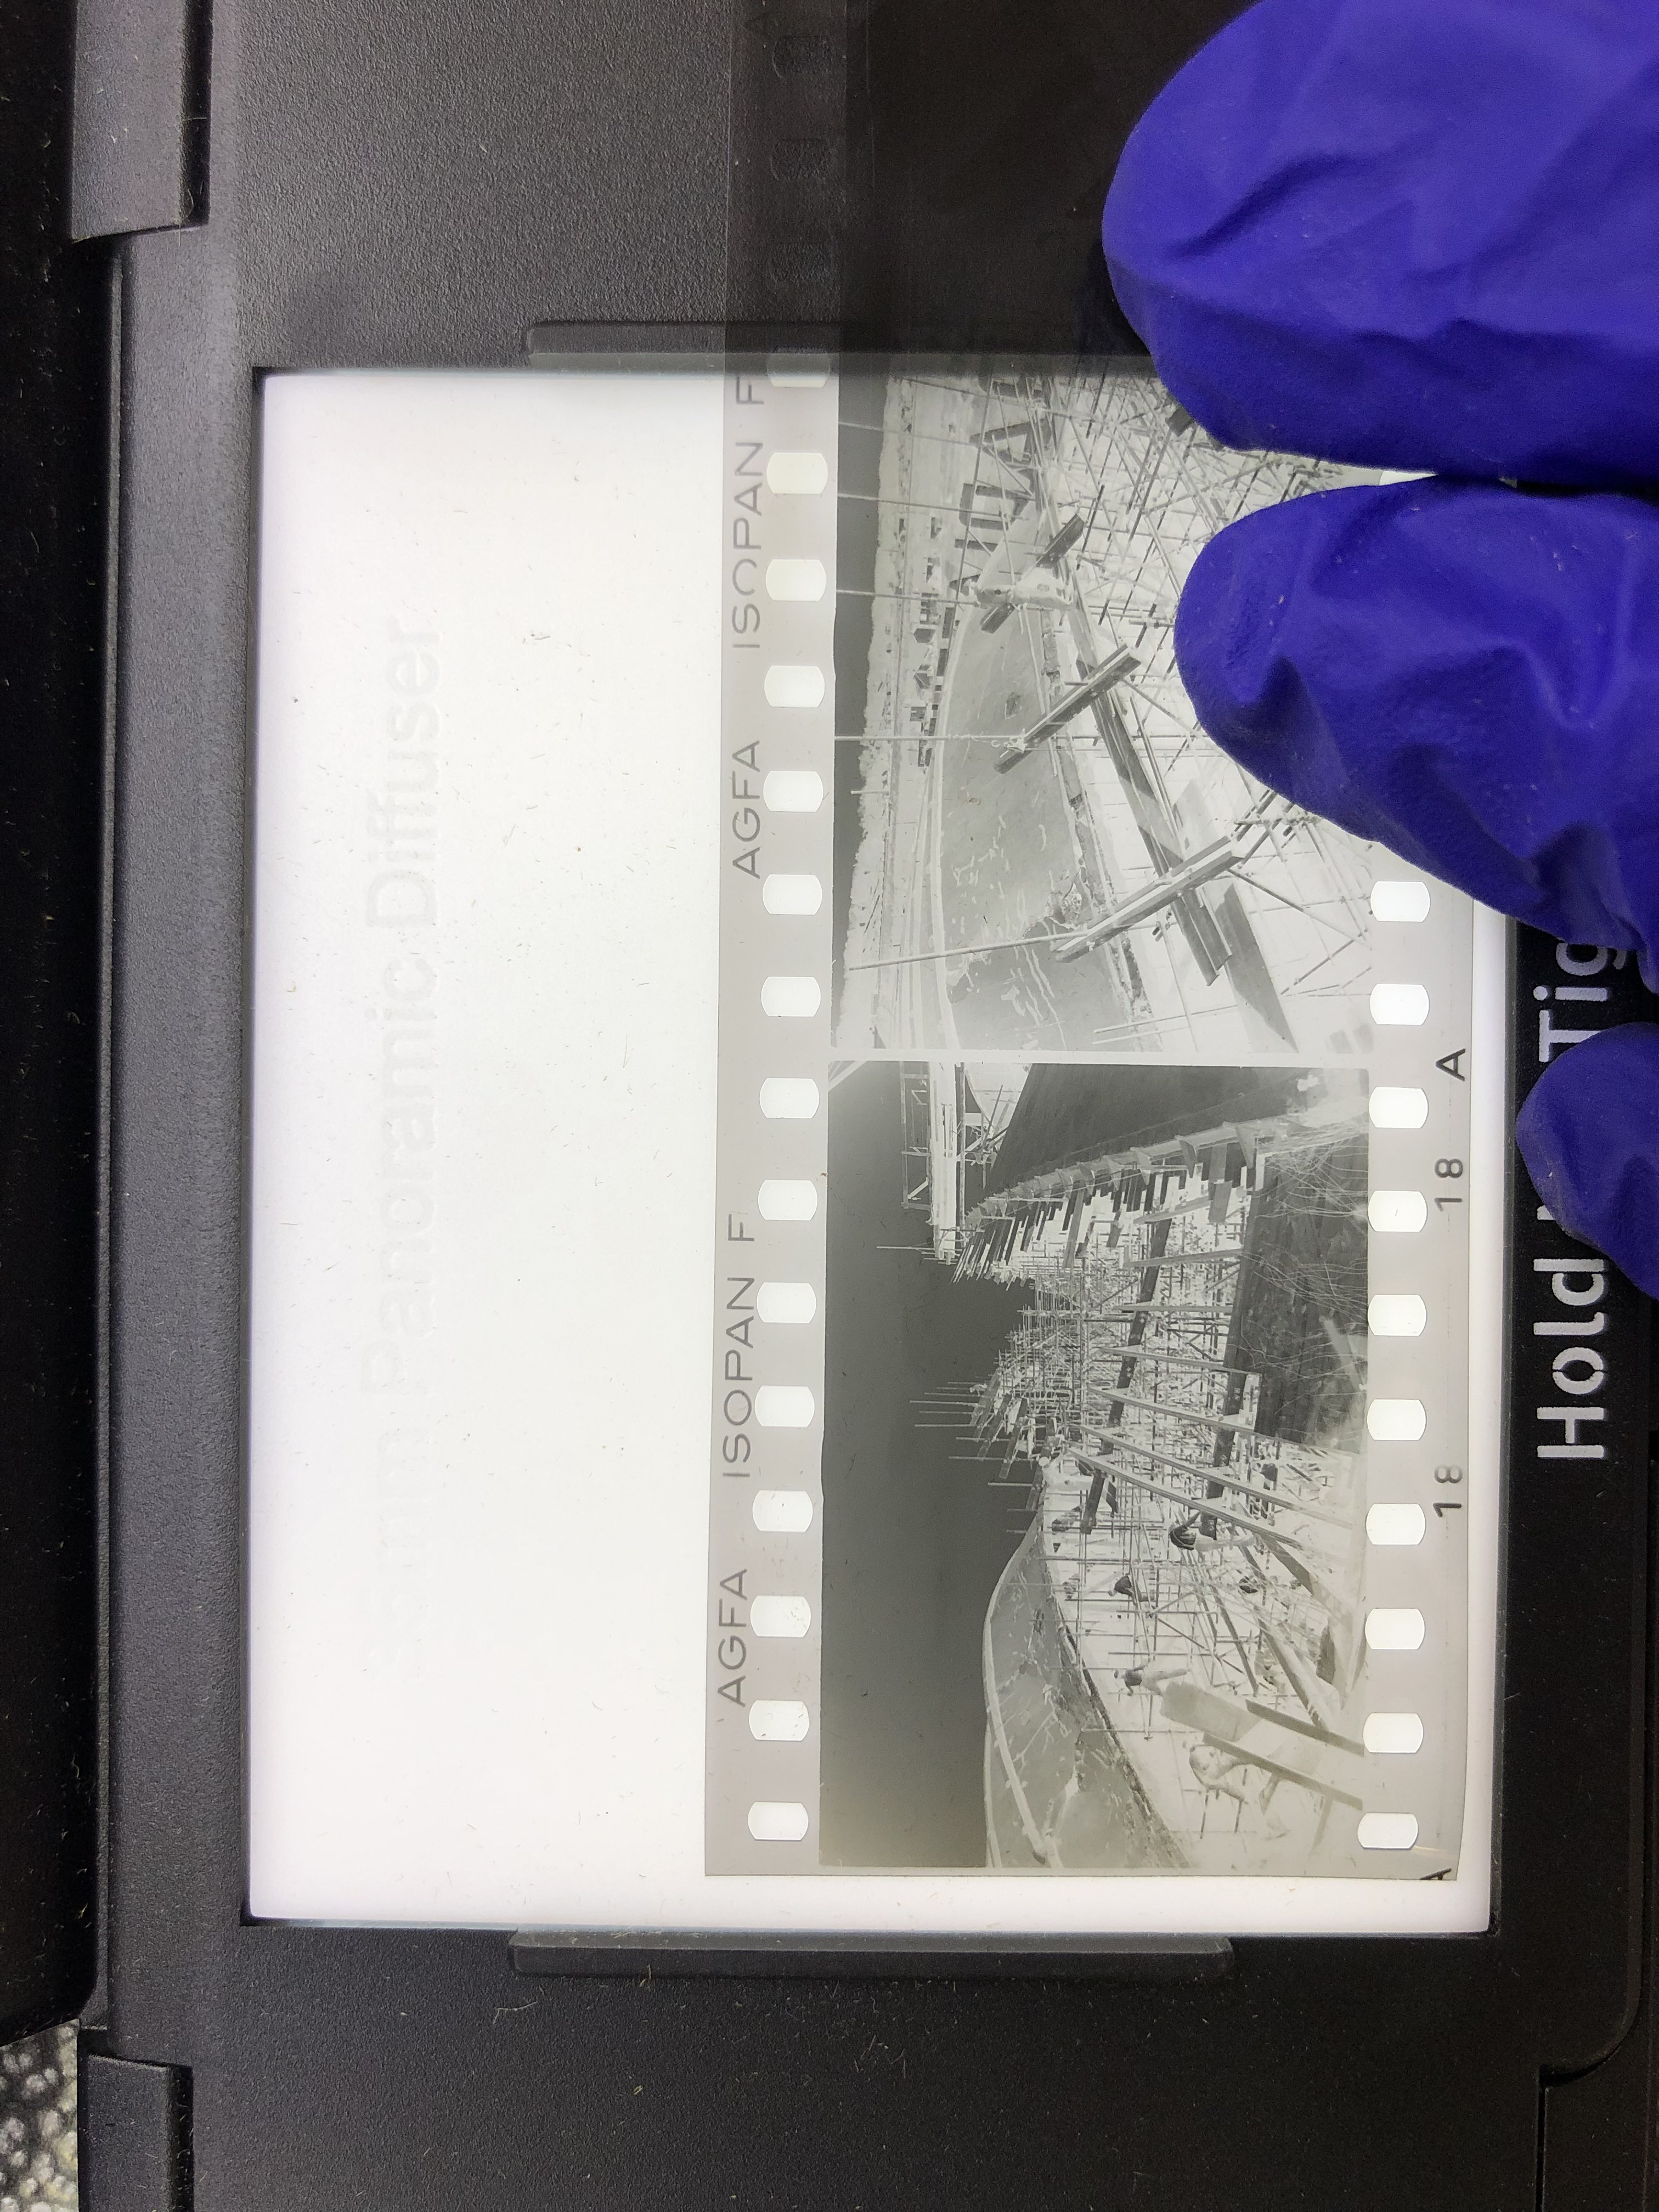
\includegraphics[width=\linewidth]{Illustrations/P9.jpg}
        \caption{}
    \end{subfigure}
    \begin{subfigure}{0.24\textwidth}
        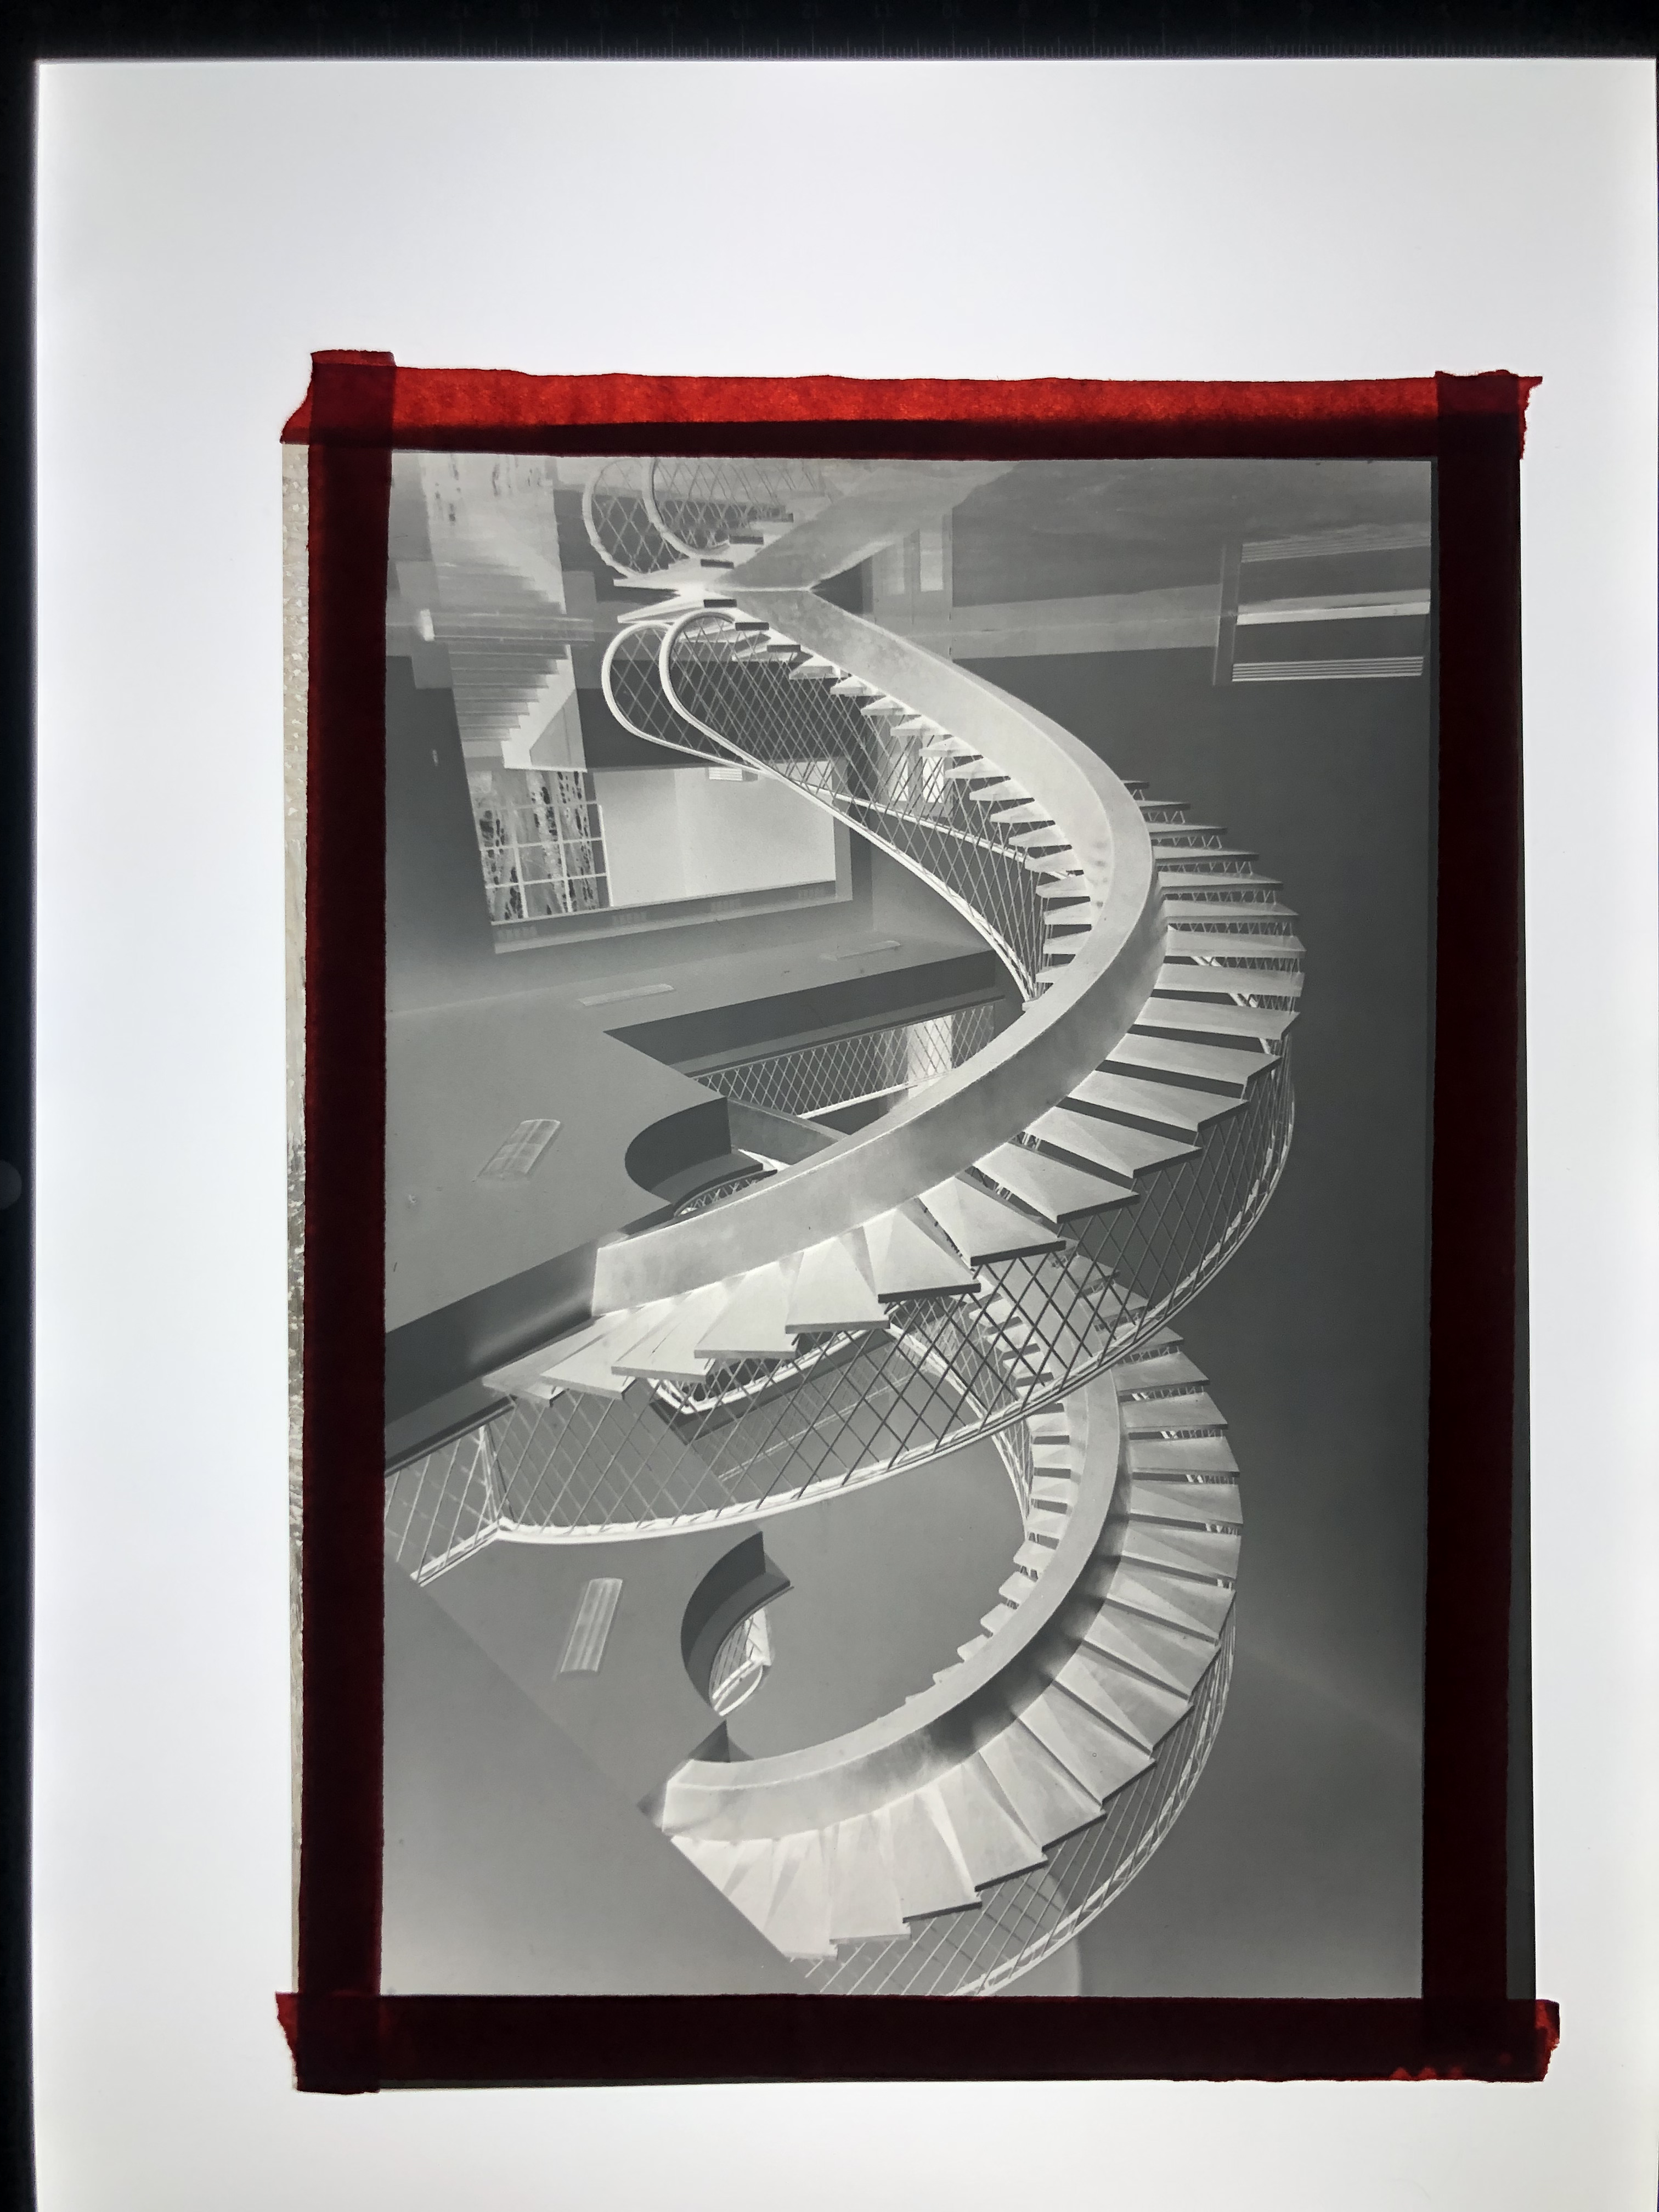
\includegraphics[width=\linewidth]{Illustrations/P10.jpg}
        \caption{}
    \end{subfigure}
    \begin{subfigure}{0.24\textwidth}
        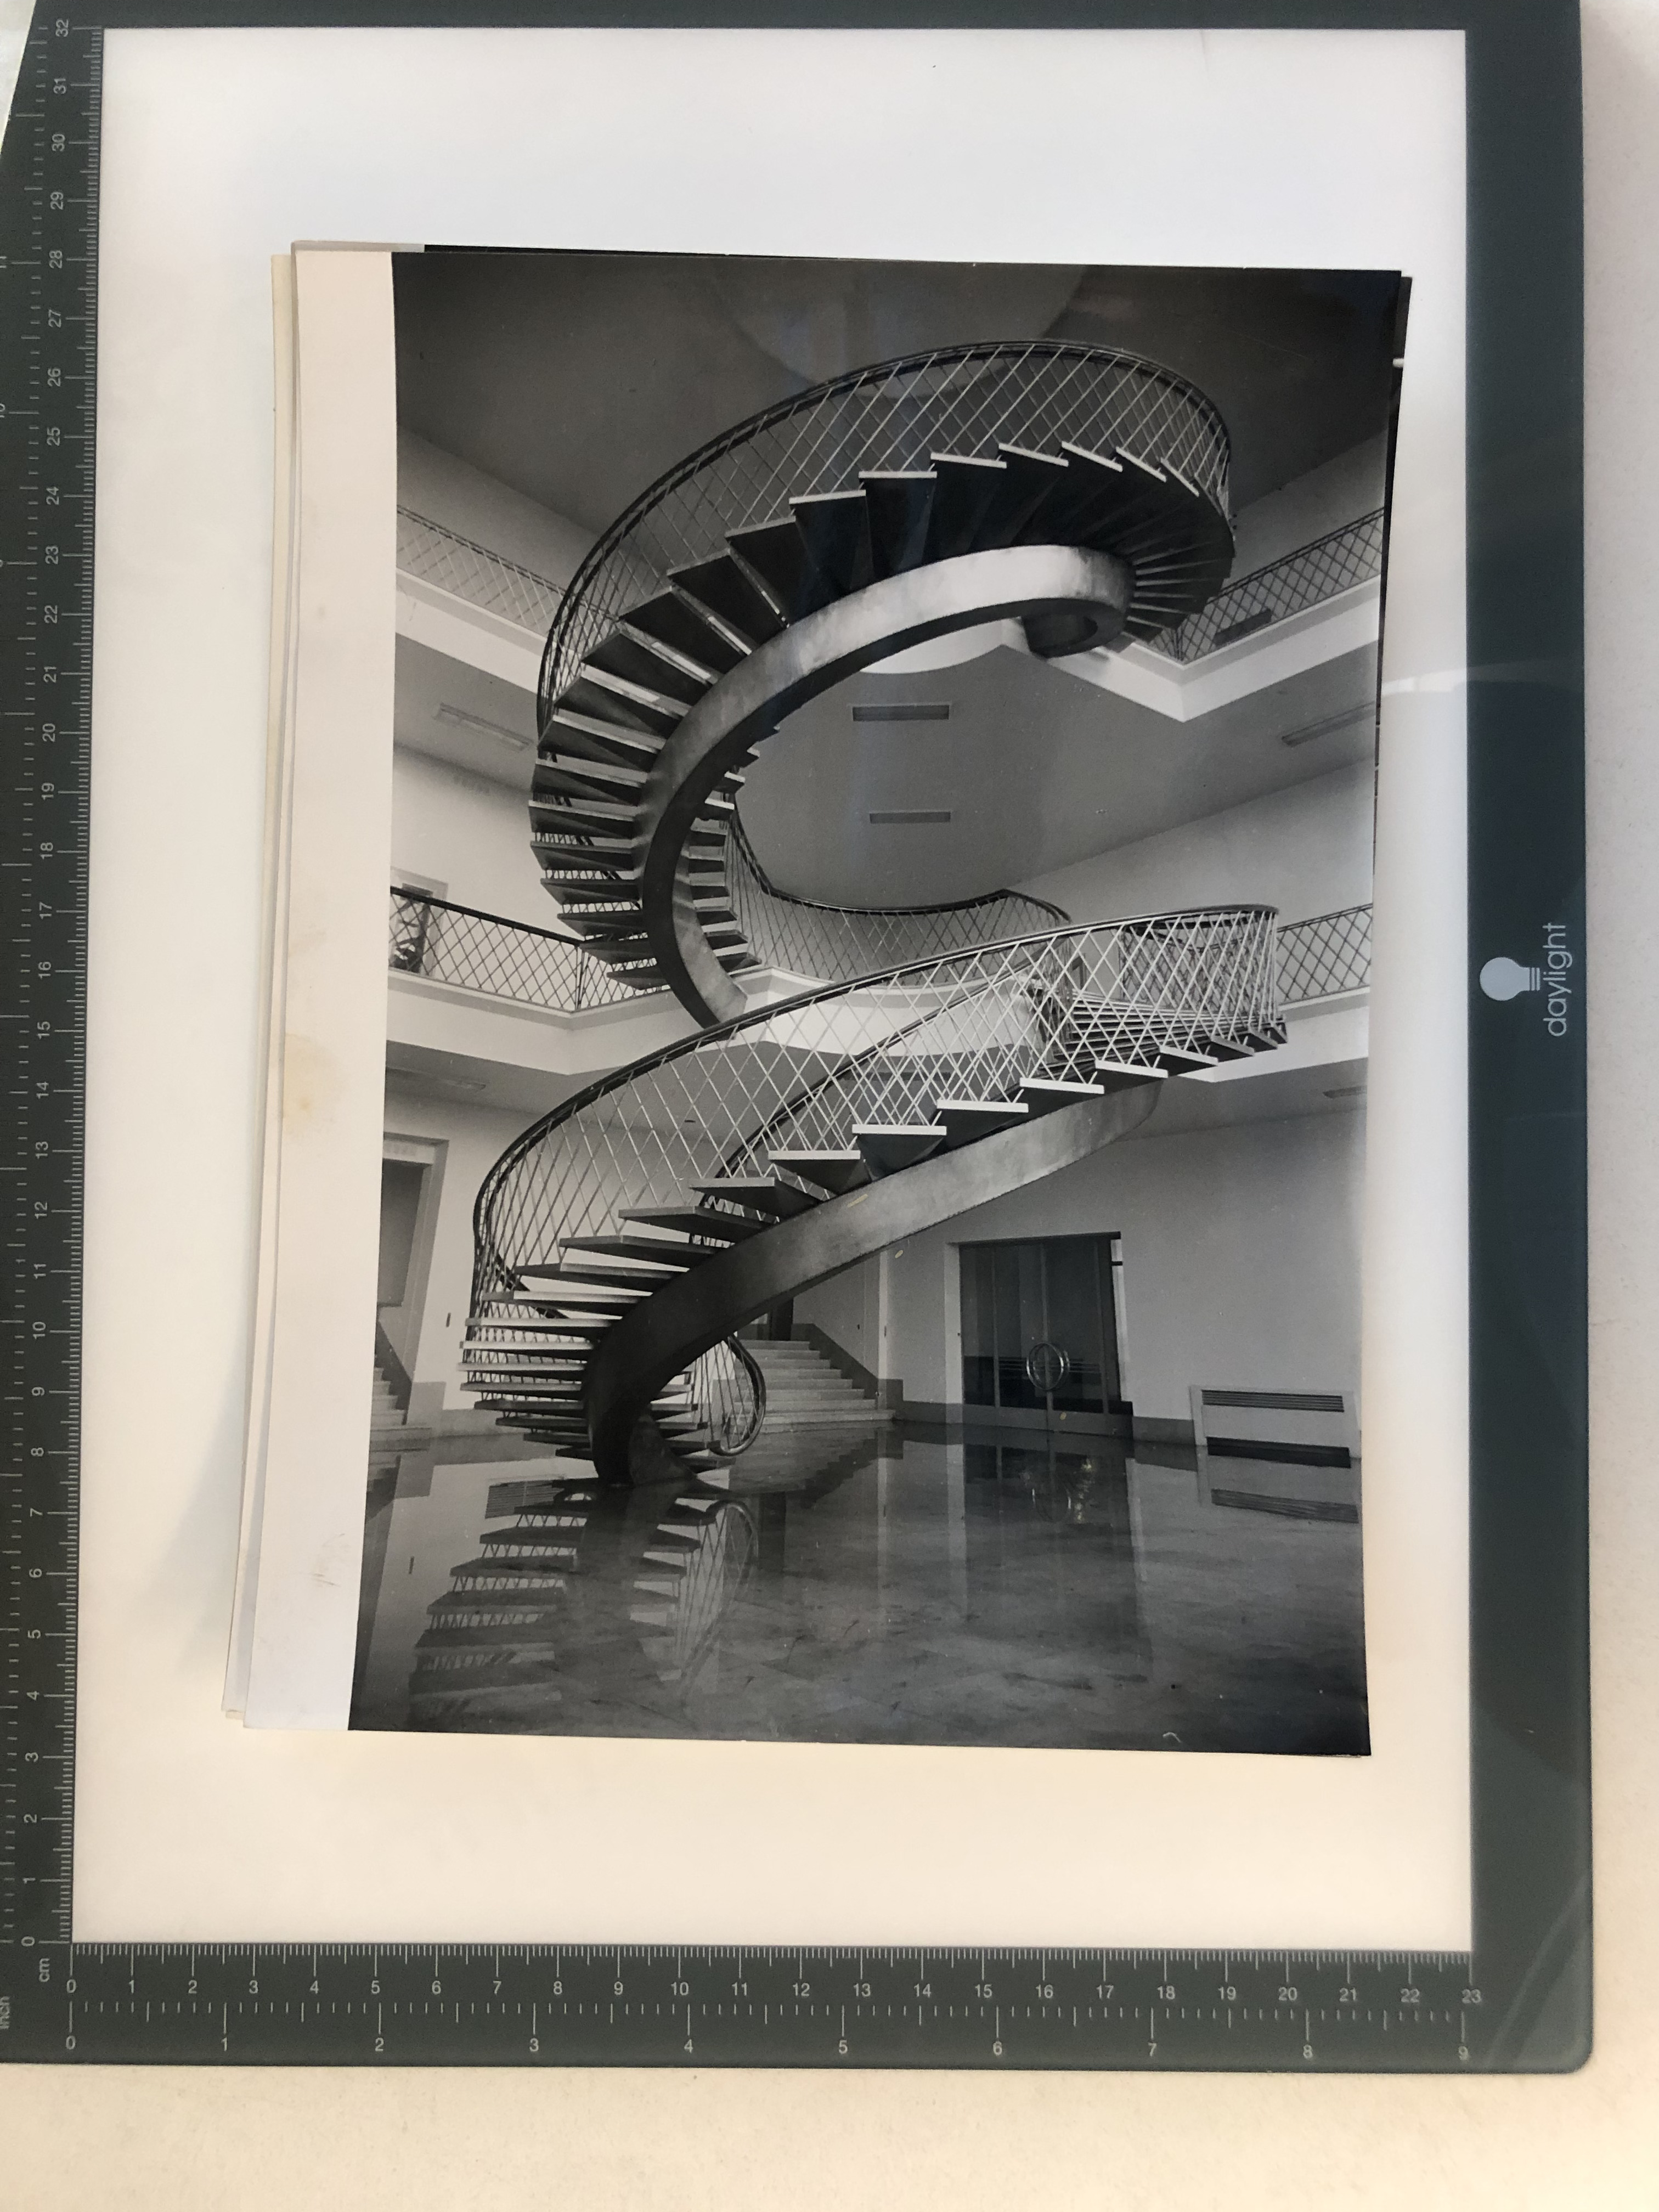
\includegraphics[width=\linewidth]{Illustrations/P11.jpg}
        \caption{}
    \end{subfigure}
    \begin{subfigure}{0.24\textwidth}
        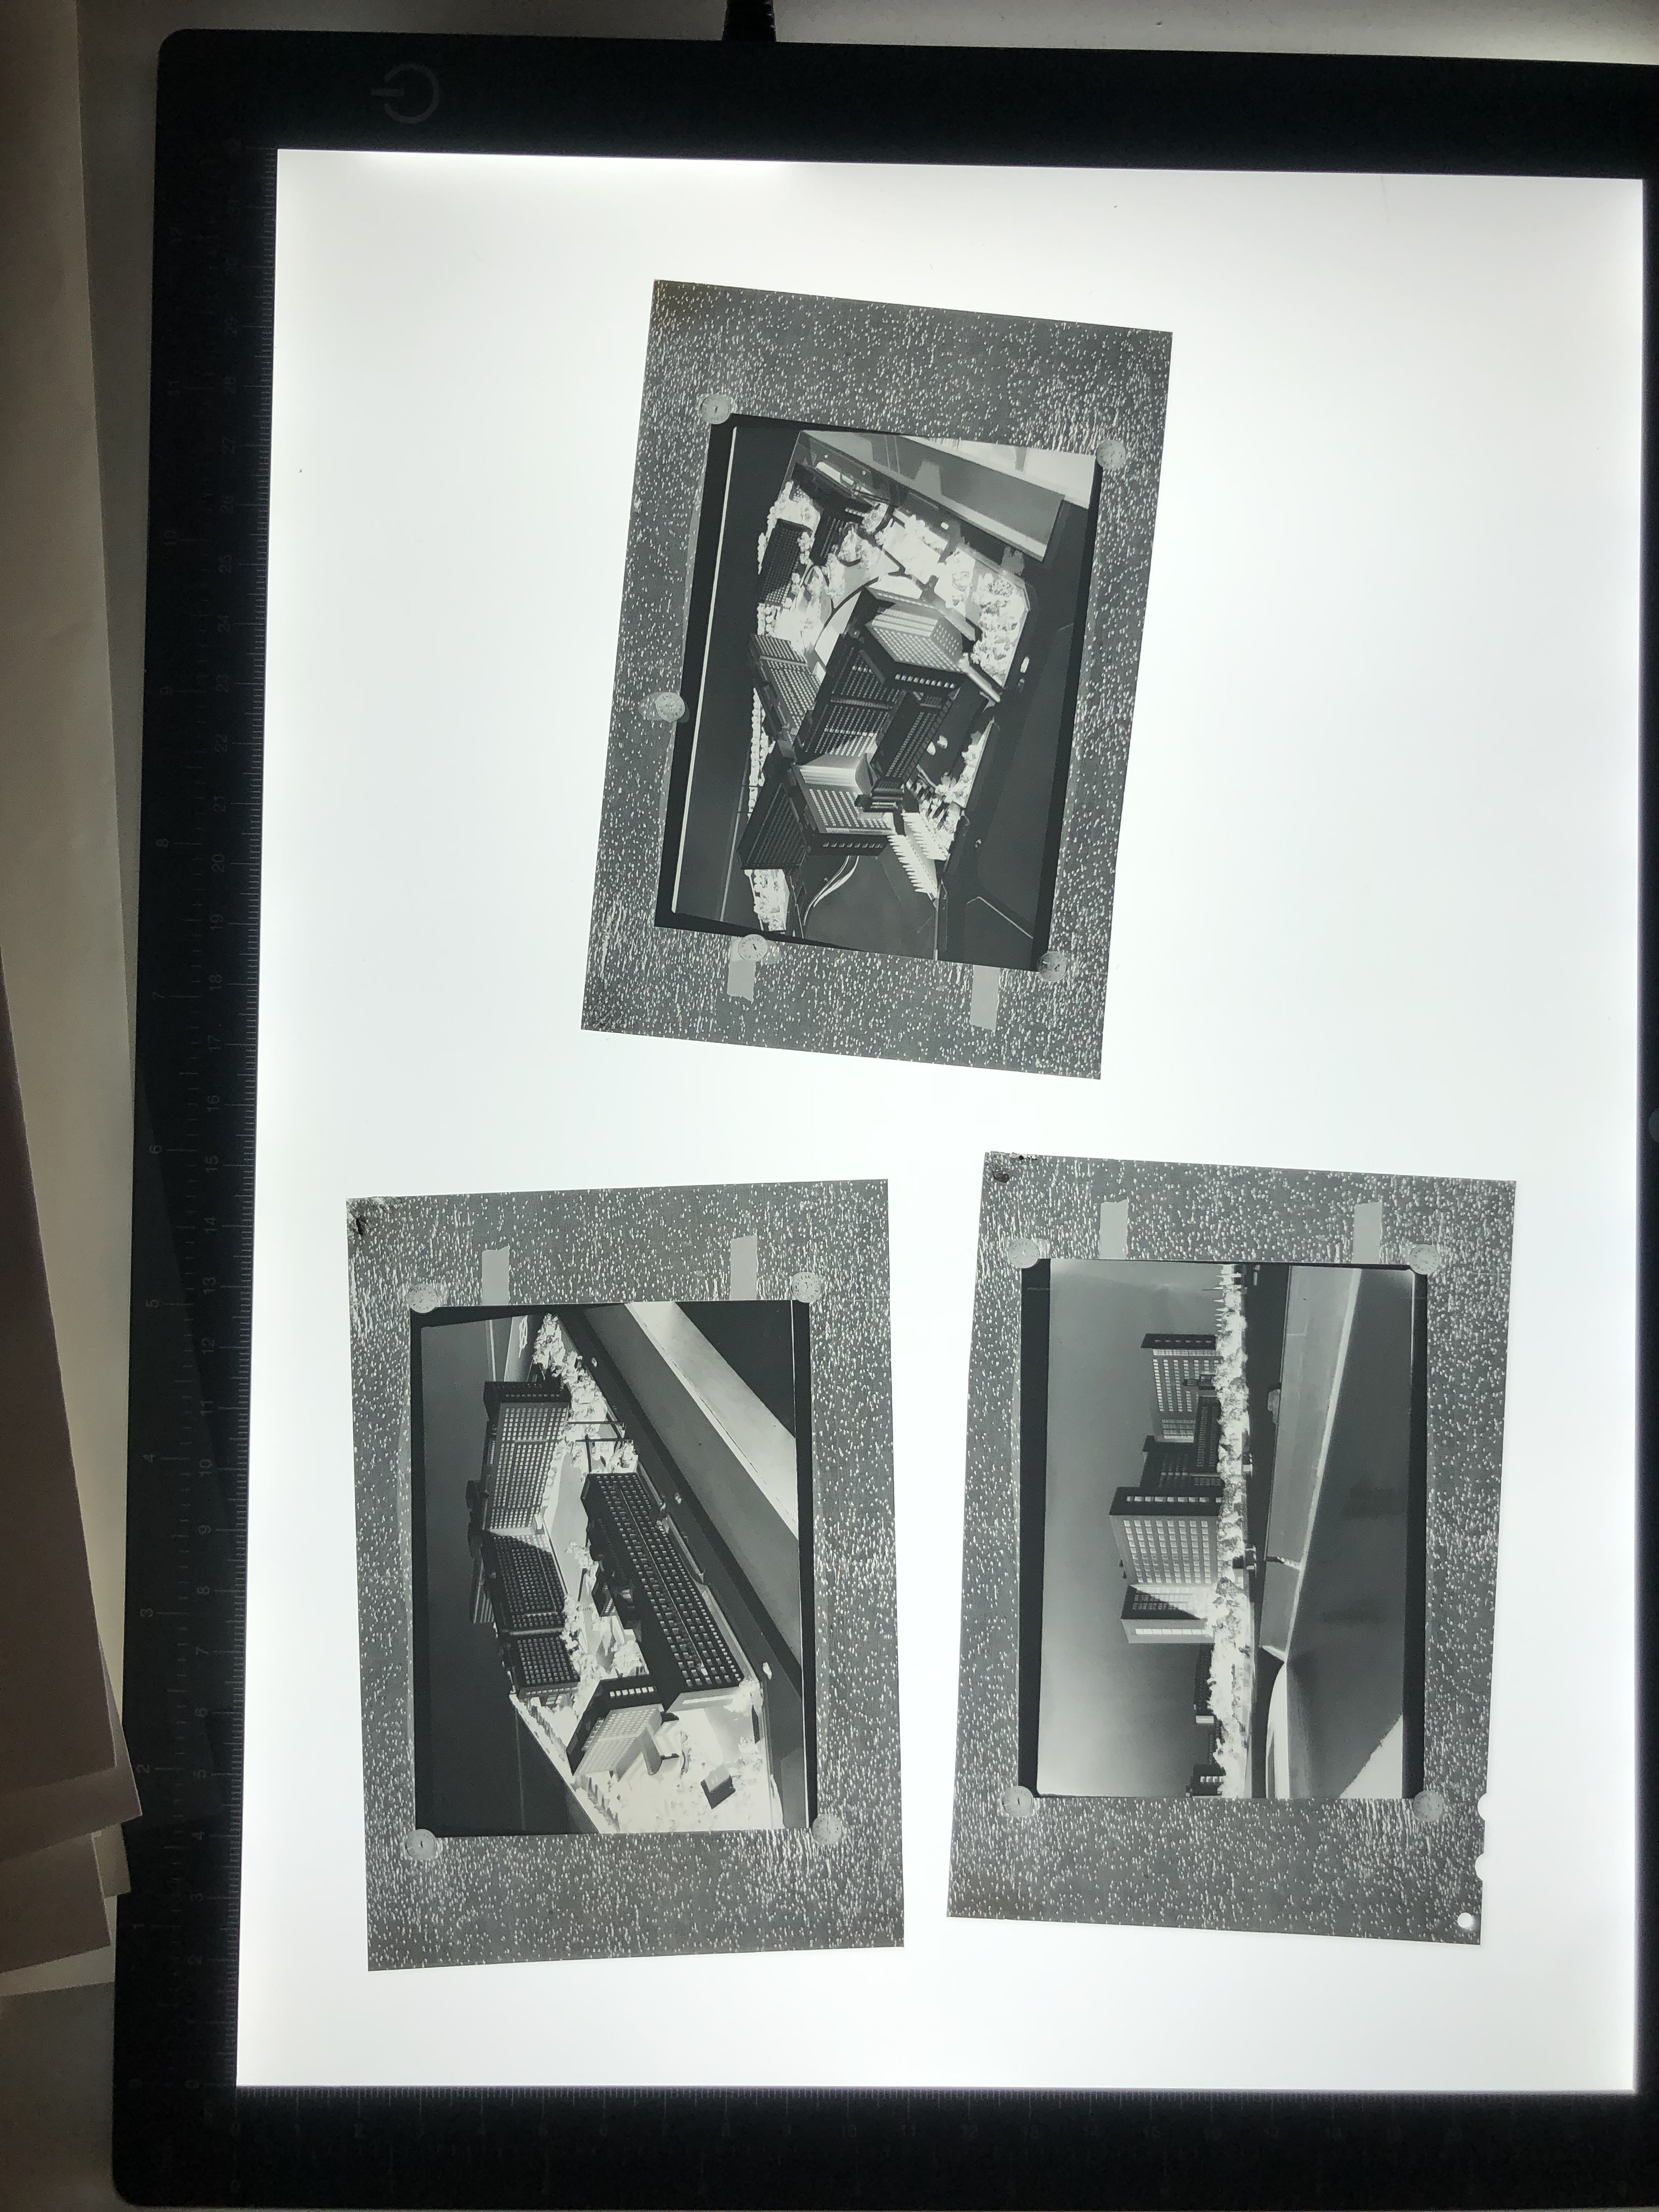
\includegraphics[width=\linewidth]{Illustrations/P12.jpg}
        \caption{}
    \end{subfigure}    
    \caption{Panorama des différents supports et formats d'images}
    \label{fig:pellicules}
\end{figure}    

Il y a plusieurs enjeux majeurs avec cette réalisation technique, tout d'abord le nommage des fichiers est en majeure partie un simple chiffre incrémenté de 1 en 1, n'offrant aucune information sur la bobine à laquelle appartenait la photo. Quelques rares photos comportent des noms de lieux, de commanditaires, des acronymes de sociétés, et l'idée sera de ne pas perdre cette information et qu'elle apparaisse dans le résultat final. Le premier enjeu est donc un enjeu de nomenclature des fichiers que nous allons produire en sortie, et donc de la réflexion que nous voulons avoir sur la manière de classifier ces objets. Le deuxième enjeu est celui des formats : il existe en tout 3 formats différents d'images, les jpg, les jpeg et les HEIC, qui sont le format produit sur iOS. Il va nous falloir harmoniser ces formats en perdant le minimum d'informations possible au moment des conversions. Enfin, troisième, et plus gros enjeu, la variété des images elle-même, comme illustrée dans l'échantillon que nous avons placé dans la page précédente. On trouve des bobines déroulées placées sur un appareil, des négatifs, des positifs, des photos développées, des plaques de verres, des supports sur tables rétroéclairées. Parfois, c'est une seule image qui apparaît, parfois c'est une image et des fragments des images précédentes et suivantes sur la bobine, parfois ce sont 3 à 6 images distinctes sur une prise de vue. De plus, l'angle des photos change en fonction du moment pendant la campagne de numérisation, on voit aussi parfois apparaître les gants de la personne qui manipule les acétates. Tout cela mis bout à bout nous donne déjà la feuille de route et les objectifs que notre code est censé accomplir.

Nous utilisons un script qui se sert de Florence-2 le Vision-language Model de Microsoft\footnote{\textit{cf}. le \textbf{\hyperref[sec:Glossaire]{Glossaire}} pour le terme \enquote{\textit{Vision-language Model}}, p.~\pageref{sec:Glossaire}.}. Sur le serveur JupyterHub du musée nous importons le corpus d'images, puis nous organisons en trois étapes le traitement dans un jupyter notebook. D'abord, faute de description, nous renommons toutes les images en incrémentant simplement de 1 en 1. Puis, nous passons un script pour uniformiser tous les formats d'images en .jpg. Enfin, nous faisons un prompt pour demander à Florence d'extraire et de créer des \textit{bounding box} autour de l'image ou des images qu'il détecte, de là en reprenant les coordonnées de ces \textit{bounding box}, nous automatisons le découpage des images pour les éclater en images individuelles\footnote{\textit{cf}. le \textbf{\hyperref[sec:Glossaire]{Glossaire}} pour le mot \enquote{prompt}, p.~\pageref{sec:Glossaire}.}. Enfin, un dernier traitement pourrait être possible : faire passer un OCR sur les images afin de récupérer des informations à même l'image pour tenter d'en donner une description minimale dans le titre de celle-ci. \hfill\break

\subsection{Le déploiement en conteneur docker de Panoptic}

Dans le cadre des ces mises en place d'outils, il a aussi fallu réfléchir à une manière de déployer sur plusieurs postes l'outil Panoptic du CERES. Dans le cadre du stage, le SI avait configuré un poste sous Ubuntu à notre attention, qui disposait des droits administrateurs. Cependant, c'est l'exception plutôt que la règle, et la plupart des employé\wokisme e\wokisme s du musée n'ont pas les droits administrateurs sur leurs machines. Dans un premier temps, nous avions envisagé d'installer une petite interface \textit{user-friendly} pour permettre aux employé\wokisme e\wokisme s de lancer l'application avec un simple double-clic sur un raccourci du bureau\footnote{\textit{cf}. le \textbf{\hyperref[sec:Glossaire]{Glossaire}} pour le terme \enquote{\textit{user-friendly}}, p.~\pageref{sec:Glossaire}.}. Autrement, Panoptic doit se lancer en ligne de commande, après l'installation d'un environnement virtuel et les employé\wokisme e\wokisme s ne se sentaient pas à l'aise de manipuler une invite de commande. En contournant cela par un raccourci, que nous venions directement installer sur l'ordinateur, cela épargnait au moins de recourir aux droits administrateurs pour l'installation, l'application et l'environnement virtuel étant configurés dans un dossier compressé. Le raccourci lançait simplement un court script en Python qui venait exécuter les commandes bash de manière transparente pour l'utilisateur et ouvrait Panoptic dans un navigateur web. 

Il reste que la solution posait deux problèmes majeurs. D'abord, l'ordinateur des employé\wokisme e\wokisme s devait être munis de Python, et pour cela les droits administrateurs étaient requis. Nous faisions donc appel au SI qui, à distance, autorisait l'installation, ce qui aurait pu représenter une perte de temps énorme s'il fallait déployer la solution à grande échelle. Deuxièmement, il fallait que les employé\wokisme e\wokisme s mettent en place eux-même le corpus qu'ils voulaient traiter en le copiant depuis la base sur la mémoire de leur ordinateur de travail, ce qui allait vite s'avérer intenable. \hfill \break

Grâce à la mise en place du serveur Jupyterhub, il a été possible de concevoir conjointement avec le SI, un déploiement de l'outil via l'intranet du musée. Un port http a été dédié au conteneur Docker contenant l'application Panoptic, ce qui le rendait accessible via une simple adresse URL à tous les postes connectés au réseau interne du musée. Il y avait donc une seule configuration unique à faire pour que tous\wokisme tes y aient accès. Aussi, cette conteneurisation du déploiement a permis de régler le second problème qui s'était posé : l'accès aux données du musée et le stockage. Le SI a pu monter directement en lecture seule les volumes de stockages principaux du musée. Cela permet de garder les arborescences que les employé\wokisme e\wokisme s connaissent déjà, et de ne pas avoir à dédoubler les données, en plus de permettre d'exporter les métadonnées que le personnel scientifique aura associé avec les bons chemins et numéros d'inventaire. 

Cependant, l'instance unique de Panoptic implique que tout le monde a accès aux projets des uns et des autres. L'idée de remonter à chaque fois un Docker avec les volumes en lecture etc,... serait trop chronophage pour le SI. Les concepteurs de l'outil n'avait pas pensé à faire un système de comptes, de log-in et de droits parce qu'ils n'en avaient pas l'utilité. Nous avons eu la chance de nous entretenir avec eux à propos de leur outil le 2 juillet 2025, notamment avec Édouard Brouté et Samuel Goncalves, afin de poser nos questions et de faire nos premiers retours sur les tests que nous avions déjà menés. Tout d'abord, le projet est un projet \textit{open-source} ce qui signifie que nous pourrions parfaitement implémenter un système d'authentification et de comptes pour remédier au problème de l'instance unique\footnote{\textit{cf}. le \textbf{\hyperref[sec:Glossaire]{Glossaire}} pour le terme \enquote{\textit{open-source}}, p.~\pageref{sec:Glossaire}.}. De plus, leurs explications étaient précieuses afin de mieux comprendre l'outil et certaines de ses limitations dans le domaine patrimonial. L'outil a été pensé pour des données nativement numériques, c'est-à-dire pour un objet image et non pour une chose photographiée. 

Ce point expliquera par la suite certains regroupements que fit l'outil pendant les tests où, par exemple, la disposition physique des objets pour des photos documentaires était jugée déterminante pour le rapprochement par similarité. C'est un point important pour le traitement de collections patrimoniales, mais un point qui peut être mitigé, ou bien même tourné à notre avantage grâce à une seconde caractéristique de l'outil : sa capacité à recevoir des plug-in et des modifications. Dans son architecture est pensée la possibilité d'ajouter des modules personnalisés, ce qui ouvre l'opportunité de brancher un modèle Clip entraîné spécifiquement sur des fonds patrimoniaux et des photos documentaires afin d'améliorer la pertinence des regroupements\footnote{\textit{cf}. le \textbf{\hyperref[sec:Glossaire]{Glossaire}} pour le terme \enquote{\textit{plug-in}}, p.~\pageref{sec:Glossaire}.}. Cela pourrait servir par exemple à repérer les dégradations, corrosions, déchirures et autres avaries sur les documents et les regrouper ensemble. Ils soulignent aussi que les étapes de tri et le processus itératif de description et caractérisation des images est indispensable parce que les premiers regroupements génèrent du bruit\footnote{\textit{cf}. le \textbf{\hyperref[sec:Glossaire]{Glossaire}}, p.~\pageref{sec:Glossaire}.} et le modèle apprend au fur et à mesure qu'on attribue des catégories à des images.

\section{Des outils d'IA aux mains des équipes}

Enfin, dans cette dernière partie, nous proposons la synthèse des entretiens que nous avons menés auprès de l'équipe des Arts graphiques autour de la manipulation de 3 outils d'intelligence artificielle\footnote{\textit{cf}. la \textbf{\hyperref[sec:Entretiens_2025]{Synthèse en Annexe C}}, p.~\pageref{sec:Entretiens_2025}.}. Ces entretiens ont été enregistrés entre juillet et août 2025, et reprennent une partie des conclusions et principes posés par la campagne d'entretien de décembre 2024 menés par Marion Charpier\footnote{\textit{cf}. la \textbf{\hyperref[sec:Entretiens_2024]{Synthèse en Annexe B}}, p.~\pageref{sec:Entretiens_2024}.}. Nous citerons les similitudes et conclusions concordantes des deux campagnes et nous réservons la partie propre aux entretiens de 2024 pour le prochain chapitre.

\subsection{Les outils présentés}

Pendant notre campagne d'entretien nous avons présenté 3 outils : \textit{Synesthesia}, Panoptic et Pixplot. \textit{Synesthesia} est un outil de rapprochement par similarité développé par Robert Erdmann Professeur à l'Université d'Amsterdam engagé par le MAD pour faciliter l'exploration des collections du musée. Le second, Panoptic, est un logiciel développé par le laboratoire CERES de Sorbonne Université\footnote{\cite{noauthor_ceres_nodate}.}. Le dernier est un outil développé par la \textit{Digital Humanities Lab} de l'Université de Yale\footnote{\cite{noauthor_yale_nodate}.}. Ces trois outils utilisent des technologies de clustering par similarité, mais pas toutes de la même époque. Le projet Pixplot date de 2017 et utilise Scikit-learn et TensorFlow\footnote{\textit{cf}. le \textbf{\hyperref[sec:Glossaire]{Glossaire}} pour les termes \enquote{Scikit-learn} et \enquote{TensorFlow}, p.~\pageref{sec:Glossaire}.}. Les deux autres utilisent Clip. 

\begin{figure}[H]
    \centering
    \begin{subfigure}{0.8\textwidth}
        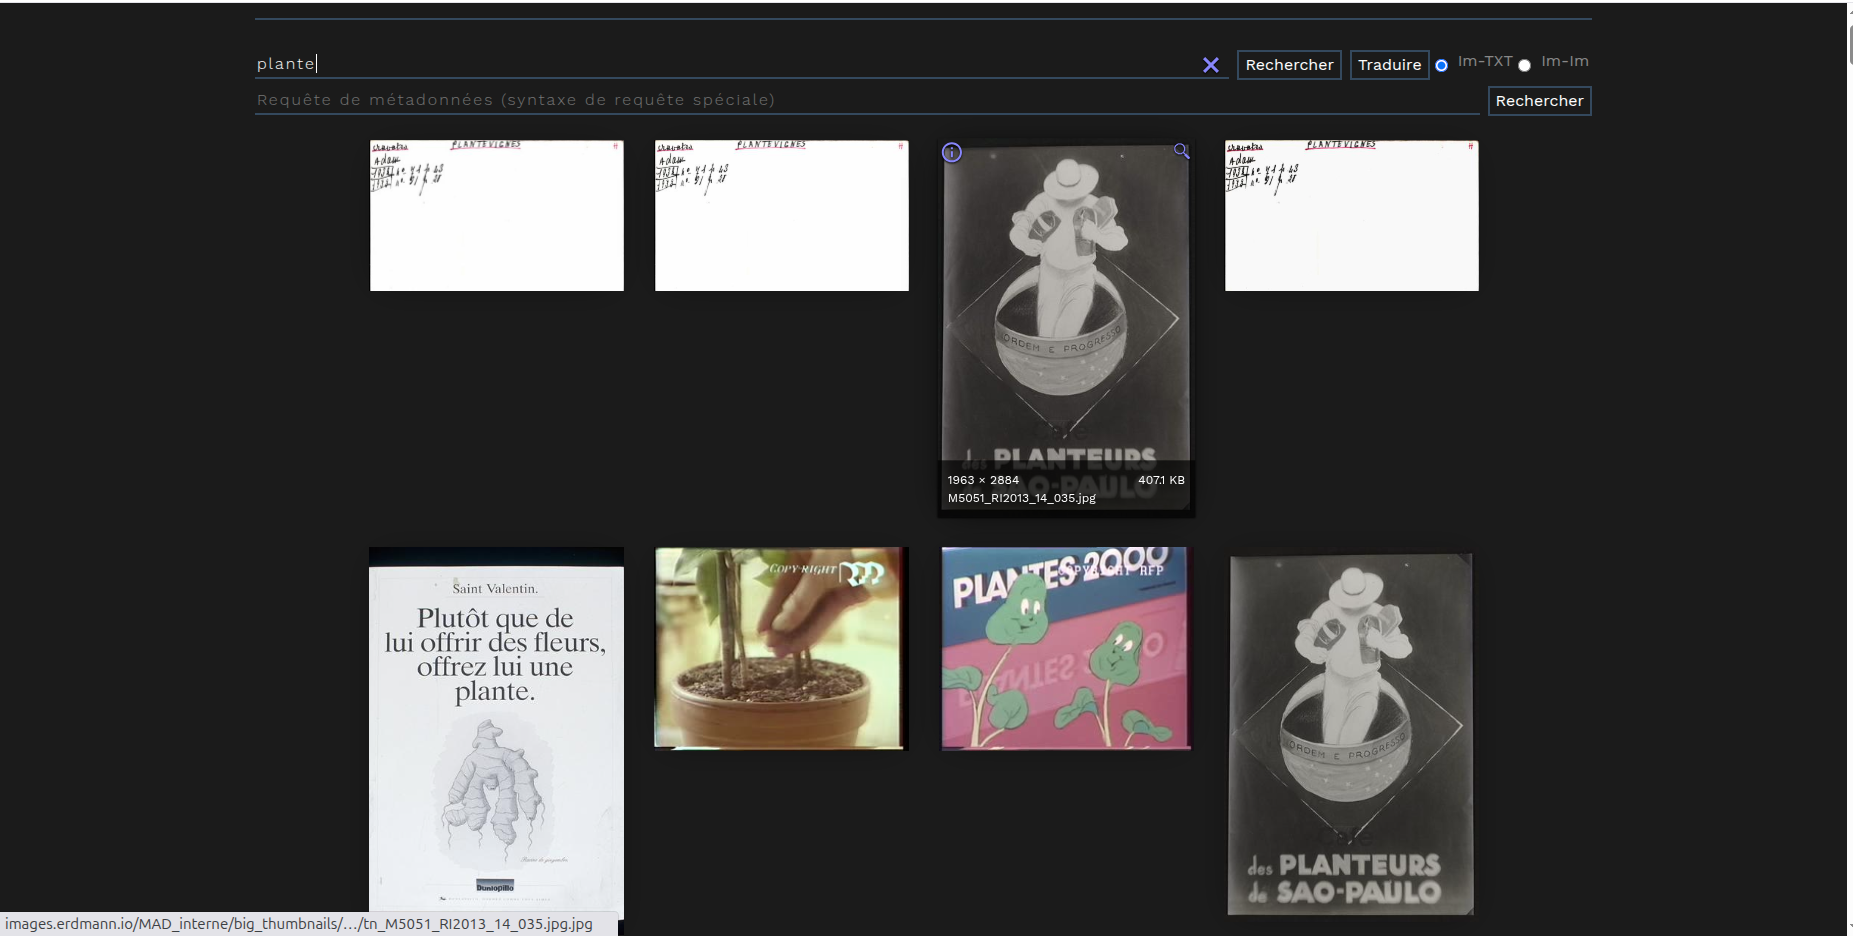
\includegraphics[width=\linewidth]{Illustrations/Synesthesia1.png}
        \caption{}
    \end{subfigure}
    \begin{subfigure}{0.8\textwidth}
        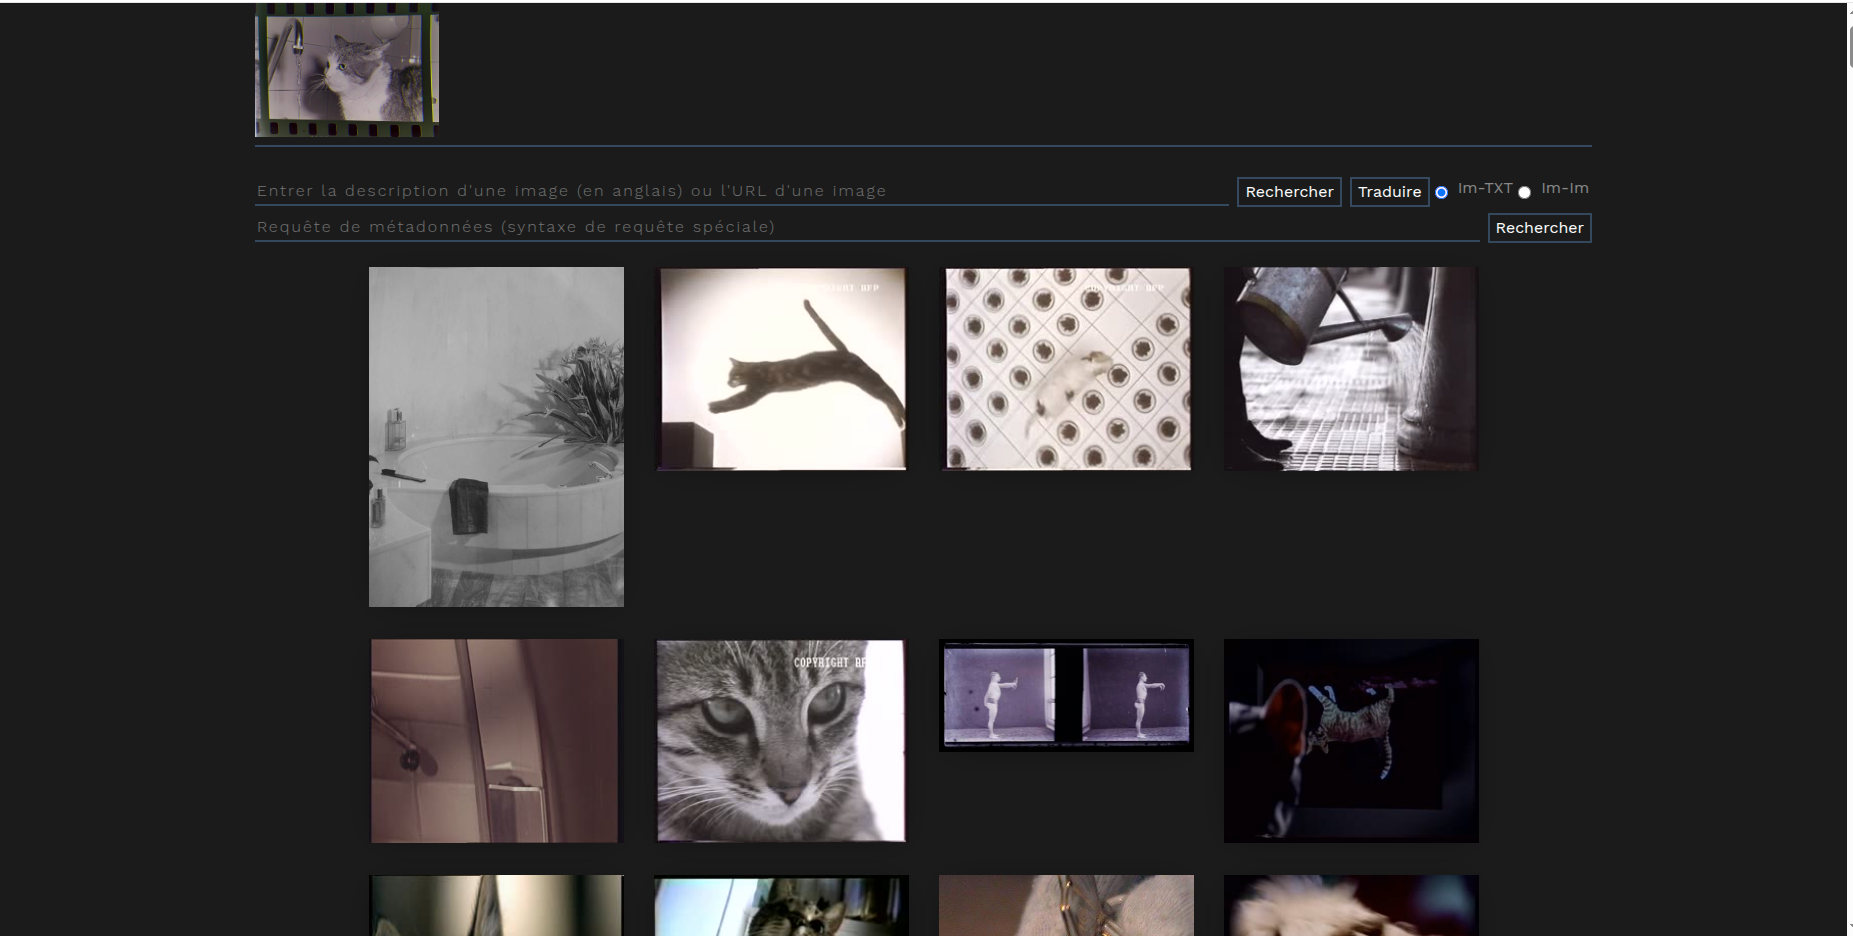
\includegraphics[width=\linewidth]{Illustrations/Synesthesia2.png}
        \caption{}
    \end{subfigure}
    \begin{subfigure}{0.8\textwidth}
        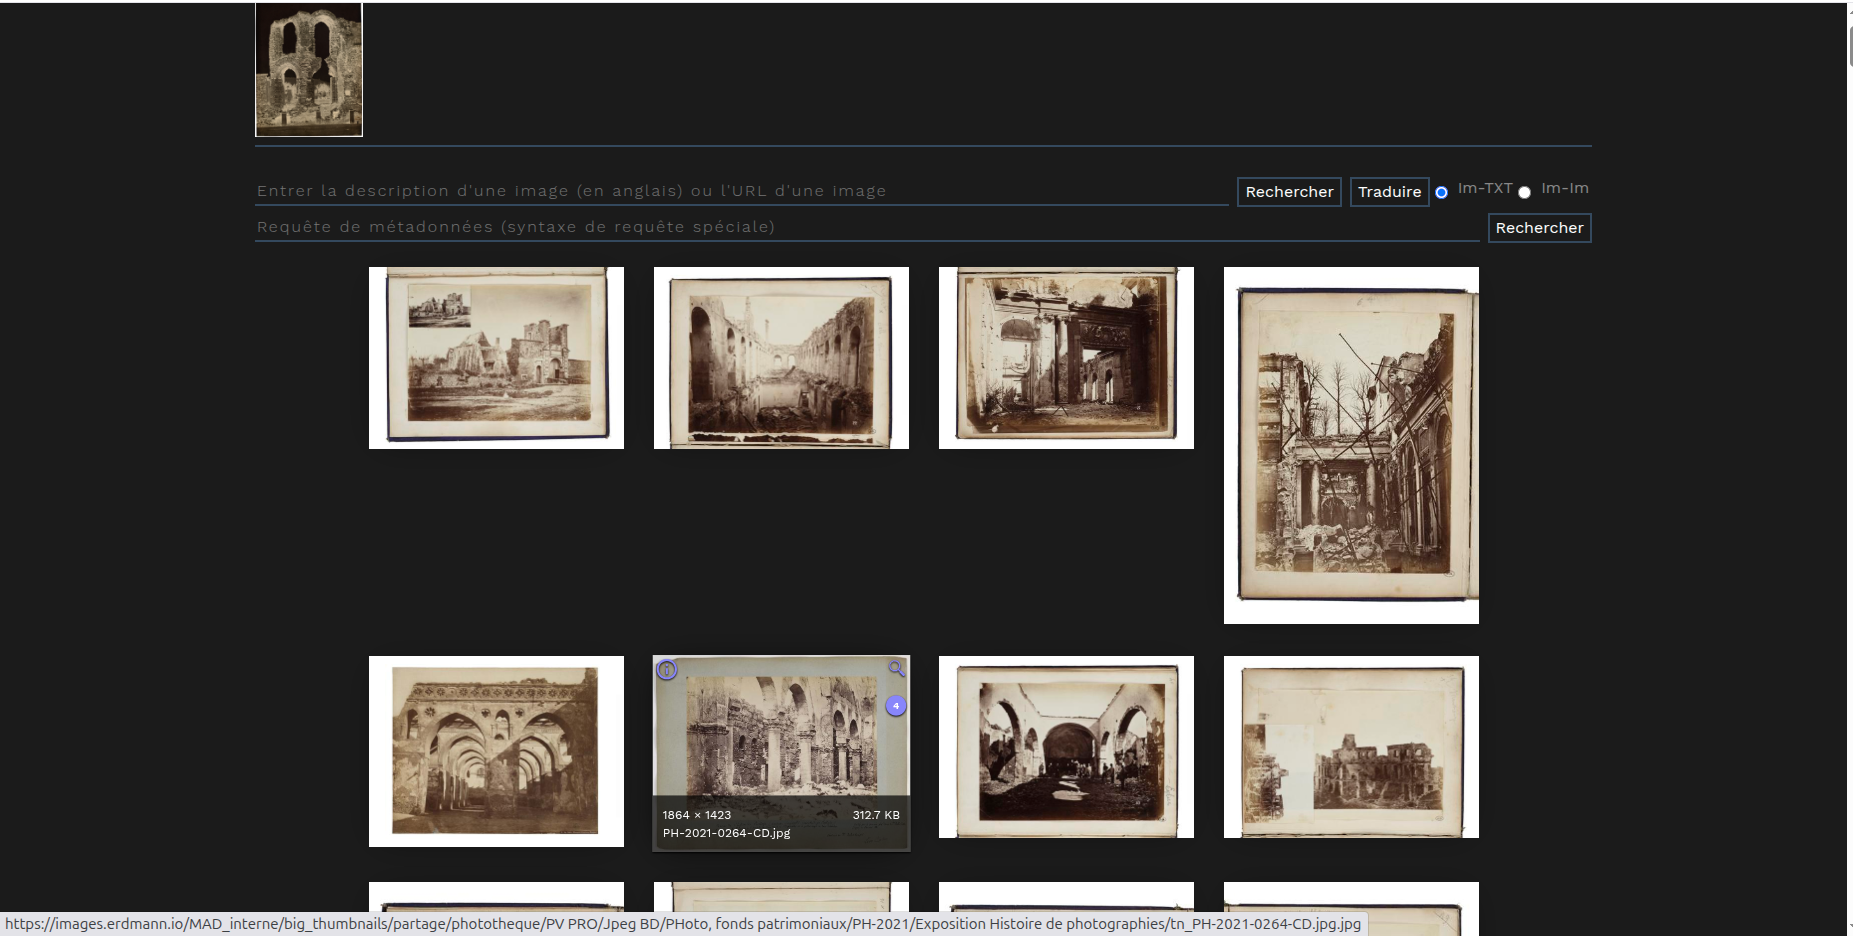
\includegraphics[width=\linewidth]{Illustrations/Synesthesia3.png}
        \caption{}
    \end{subfigure}
    \caption{Illustrations de \textit{Synesthesia}}
    \label{fig:pellicules}
\end{figure}    

Ici nous voyons quelques captures d'écrans qui illustrent le fonctionnement de \textit{Synesthesia}. L'outil consiste en un navigateur web dans lequel on peut faire des requêtes par texte, par image ou par métadonnées. L'outil est branché sur les bases du musée et montre tout ce qui est similaire ou qui correspond à la description écrite et qui se trouve dans les collections du musée. Lorsqu'on clique sur une image, l'application nous ouvre une fiche d'information qui contient le nom du fichier, son emplacement, sa taille et ses métadonnées associées. Si l’œuvre sur laquelle on clique figure dans la base de données Arcadie, alors cela nous redirige directement sur la fiche de l’œuvre dans la base. Dans les exemples donnés ici, nous avons d'abord fait une recherche par texte avec le mot \enquote{Plante}. Cette recherche nous montre autant des représentations de plantes que des documents contenant le mot recherché. Ensuite nous avons fait la recherche avec une numérisation d’œuvre qui n'est pas sur la base du musée, le chat près du robinet, et par similarité l'application a trouvé d'autres occurrences de chats dans les collections. Enfin, un négatif de photographie d'une collection qui se trouve dans les bases du musée et l'application nous a retrouvé les œuvres similaires, la plupart appartenant au même fonds.


\begin{figure}[H]
    \centering
    \begin{subfigure}{0.8\textwidth}
        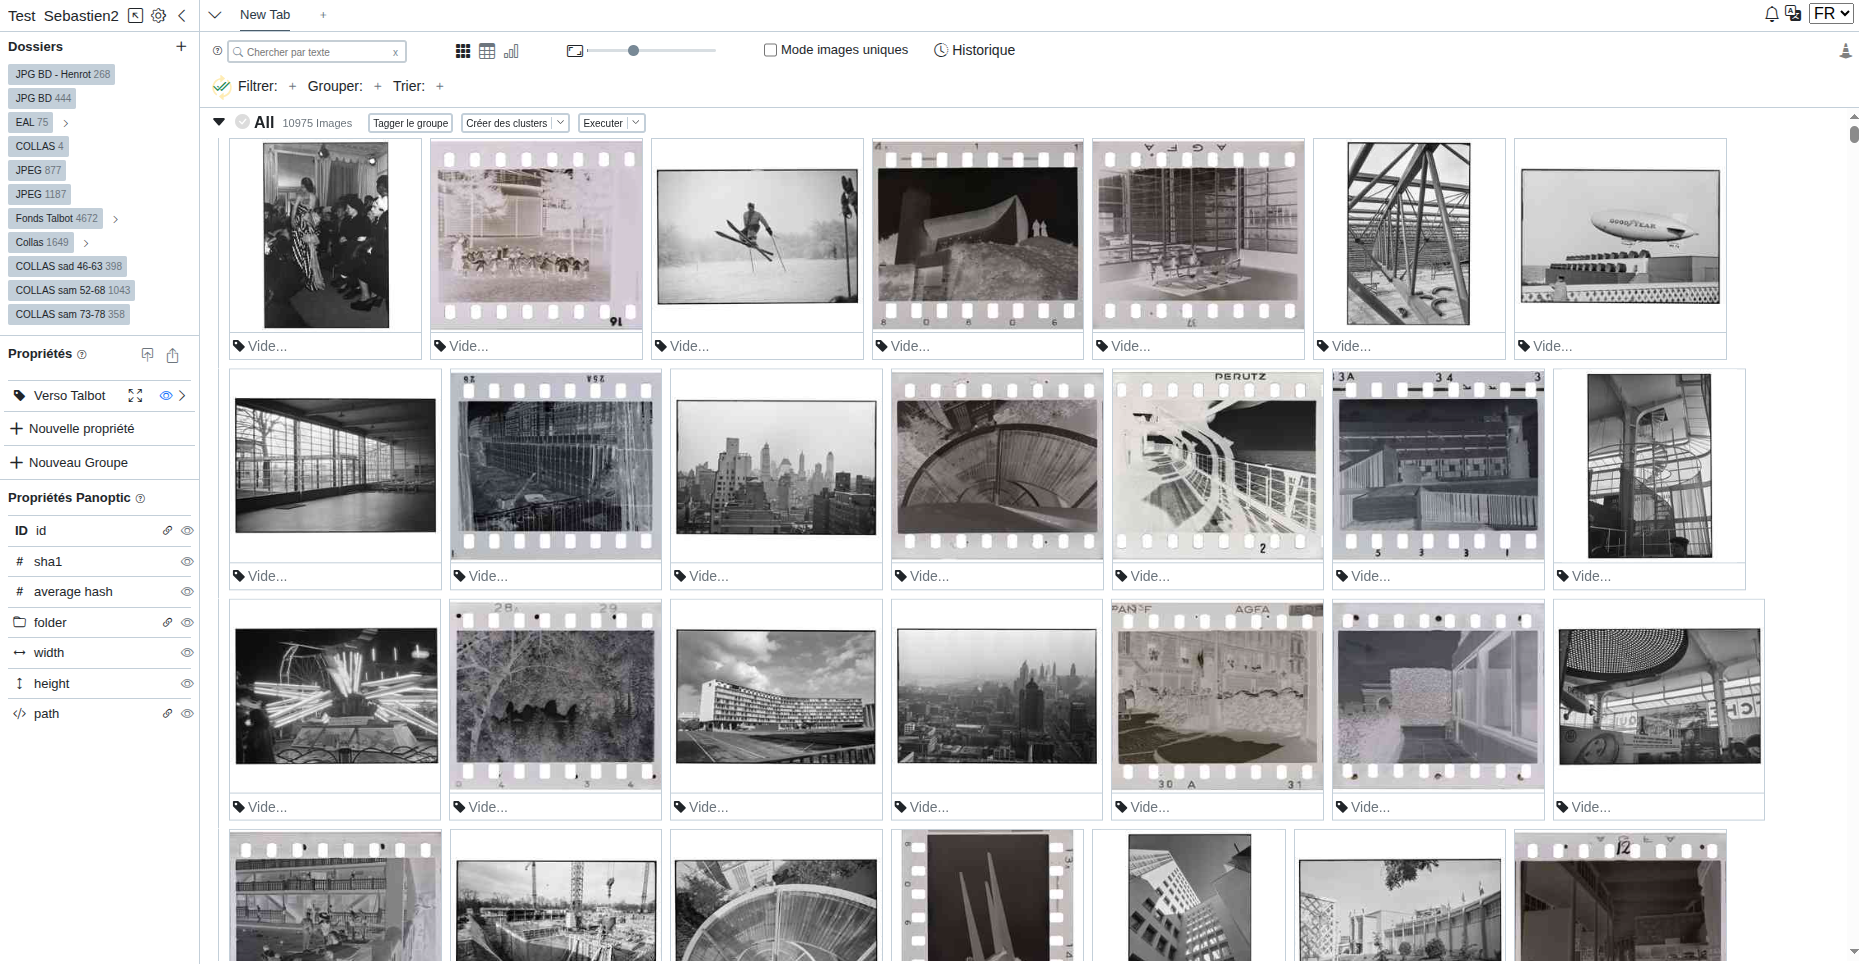
\includegraphics[width=\linewidth]{Illustrations/Panoptic1.png}
        \caption{}
    \end{subfigure}
    \begin{subfigure}{0.8\textwidth}
        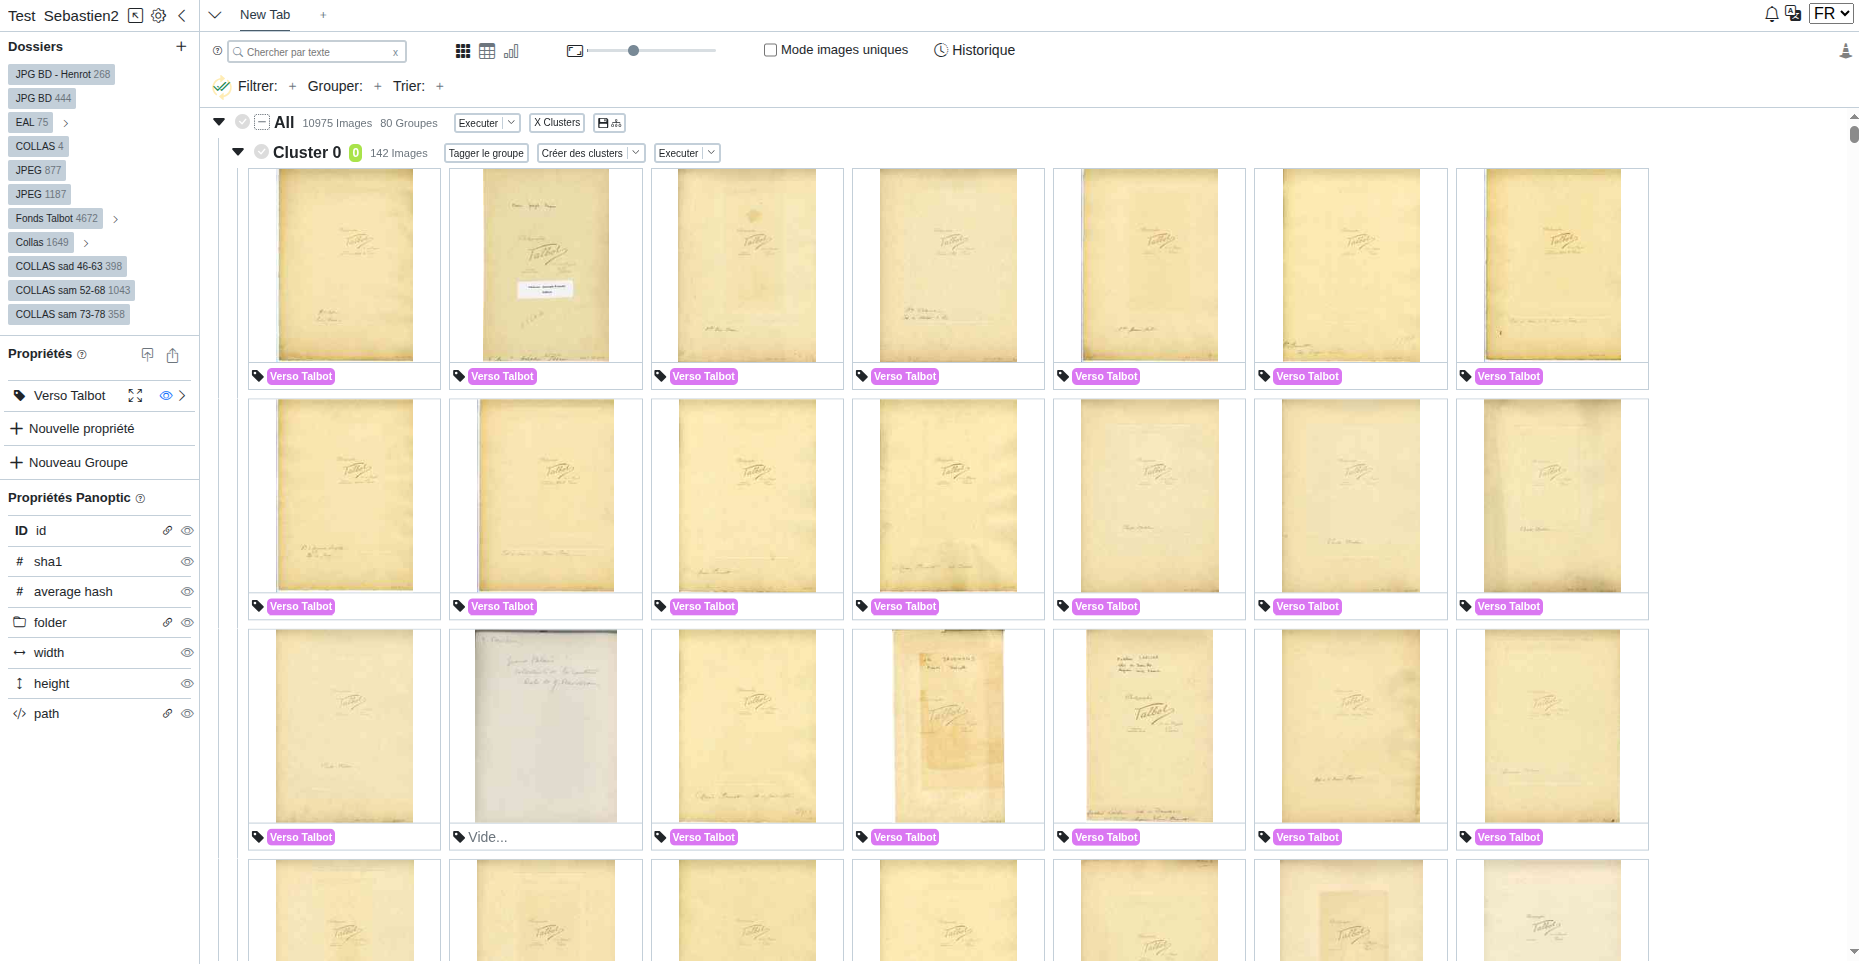
\includegraphics[width=\linewidth]{Illustrations/Panoptic2.png}
        \caption{}
    \end{subfigure}
    \begin{subfigure}{0.8\textwidth}
        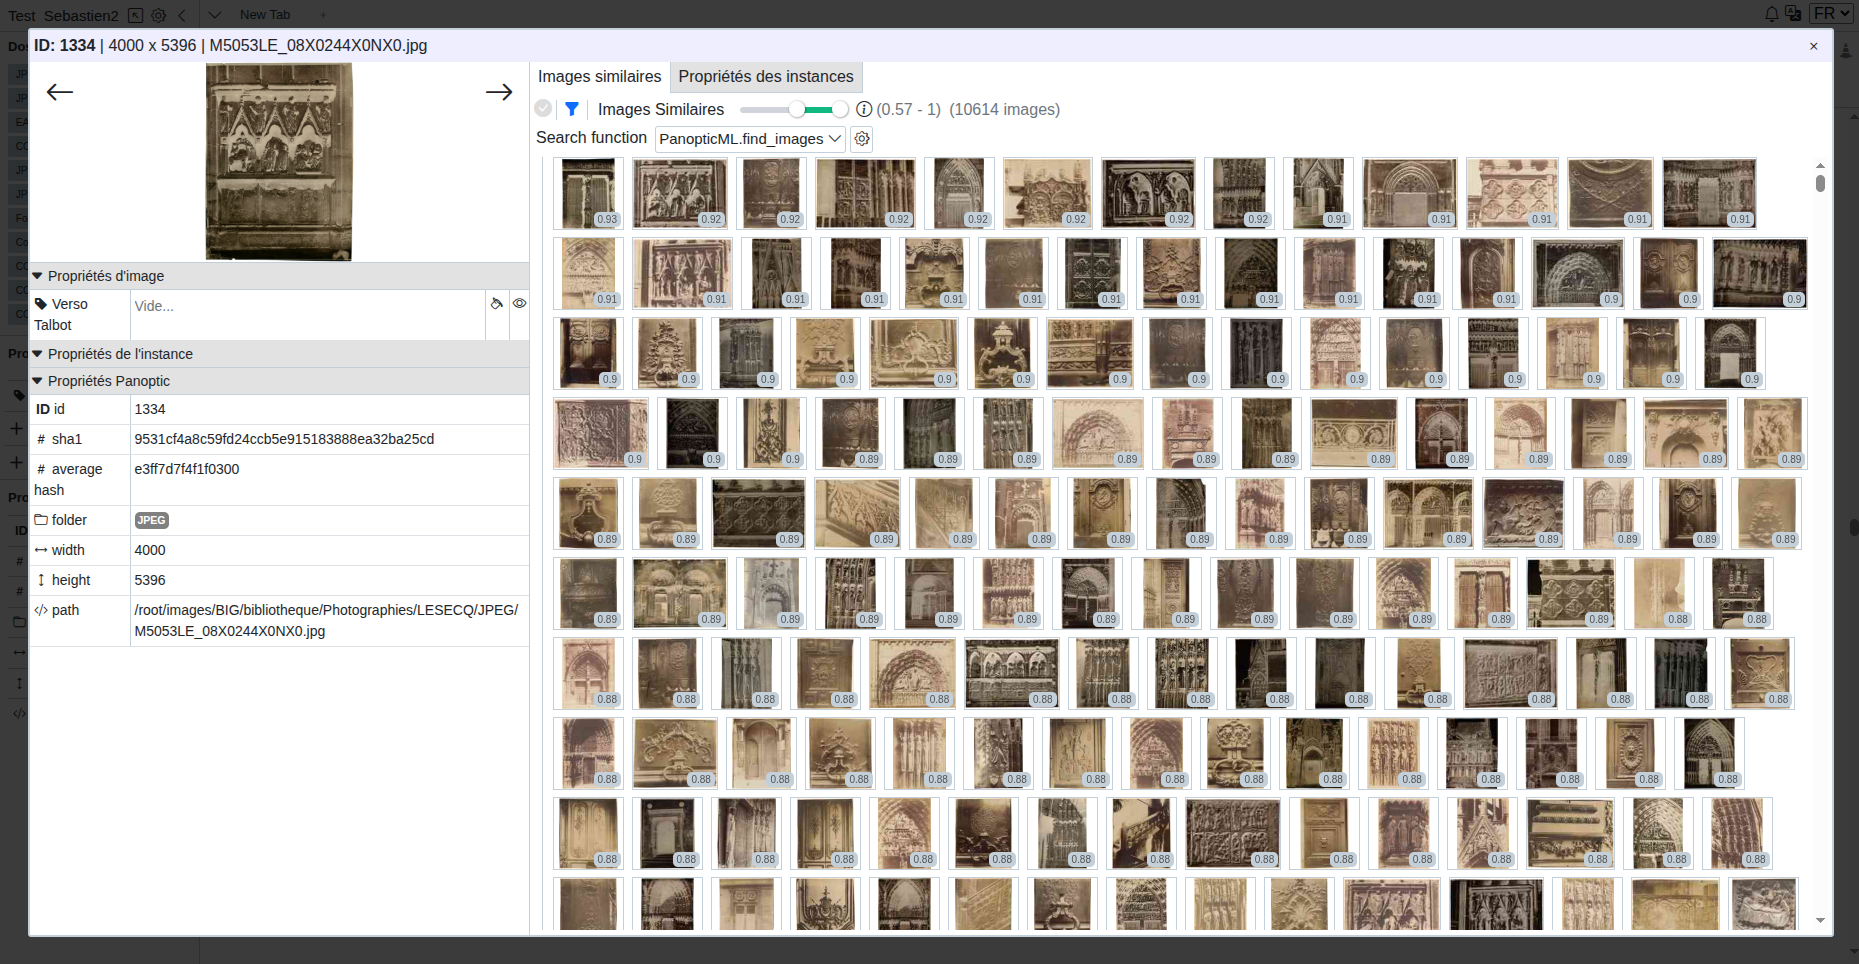
\includegraphics[width=\linewidth]{Illustrations/Panoptic3.png}
        \caption{}
    \end{subfigure}
    \caption{Illustrations de Panoptic}
    \label{fig:pellicules}
\end{figure}

De la même manière, le second outil est aussi une visionneuse d'image mais cette fois, dont le fonctionnement est différent. Ici on relie aussi les bases du musée à l'outil, on fait cependant une sélection dans les fonds puis on lance le regroupement par clusterisation. On donne à l'outil un certain nombre de regroupement à faire, imaginons 60, et il va créer des groupes avec des images qu'il pense similaire. Cet outil permet aussi de faire des recherches avec du texte, de générer les clusters en passant les images en niveau de gris. La démarche avec cet outil consiste à créer des étiquettes ou \textit{labels} et d'apposer des catégories aux images afin de décrire les œuvres. Il permet de trier, grouper ou filtrer les groupes que nous avons créés, afin de relancer la clusterisation en affinant les groupements et distinctions. La force de cet outil réside dans sa grande capacité d'absorption qui peut traiter 1 millions d'images dans un même projet, mais aussi dans la possibilité d'exporter en csv les métadonnées (les étiquettes) produites par l'agent. Cette fonctionnalité ouvre la possibilité de traiter les collections en masse, en s'aidant de la clusterisation et en gardant la maîtrise sur les données produites. Nous pouvons ainsi exporter les informations correspondantes grâce au fait que l'application garde aussi les chemins d'accès des fichiers en mémoire. Ceci évite l'écueil des mots-clefs générés par IA hors d'un vocabulaire contrôlé et qui peuvent s'avérer imprécis ou totalement erronés.


\begin{figure}[H]
    \centering
    \begin{subfigure}{0.8\textwidth}
        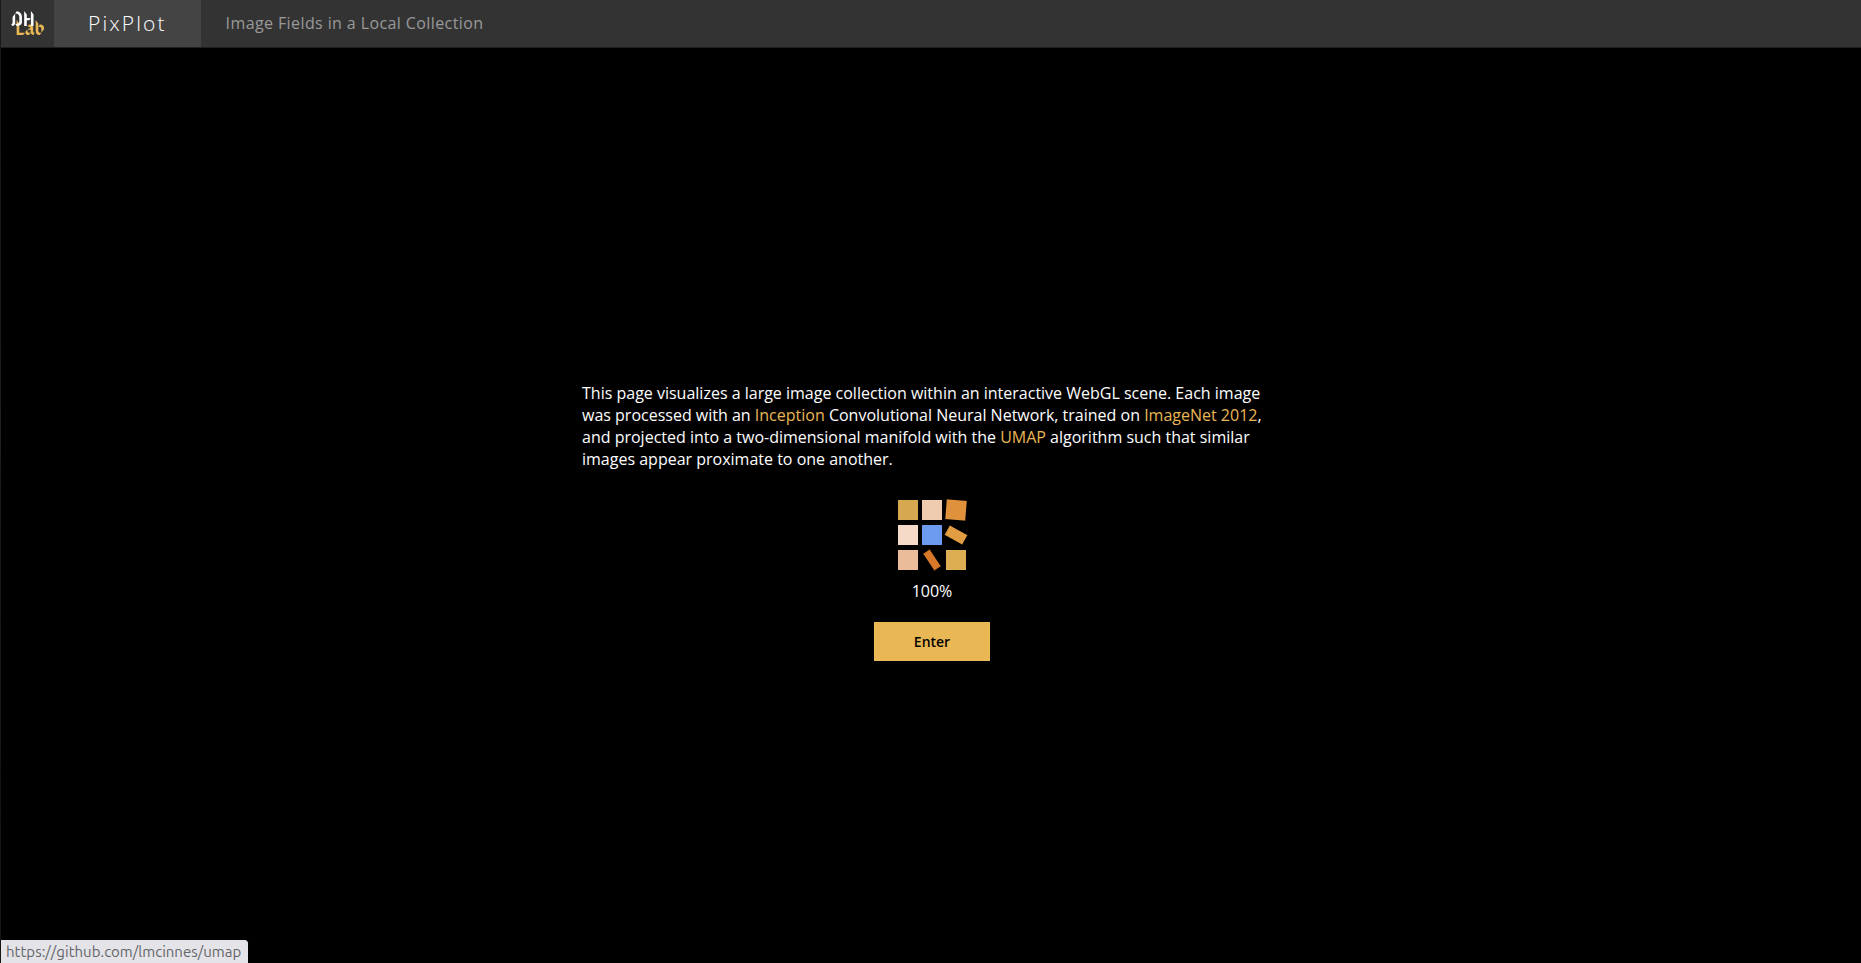
\includegraphics[width=\linewidth]{Illustrations/Pixplot1.png}
        \caption{}
    \end{subfigure}
    \begin{subfigure}{0.8\textwidth}
        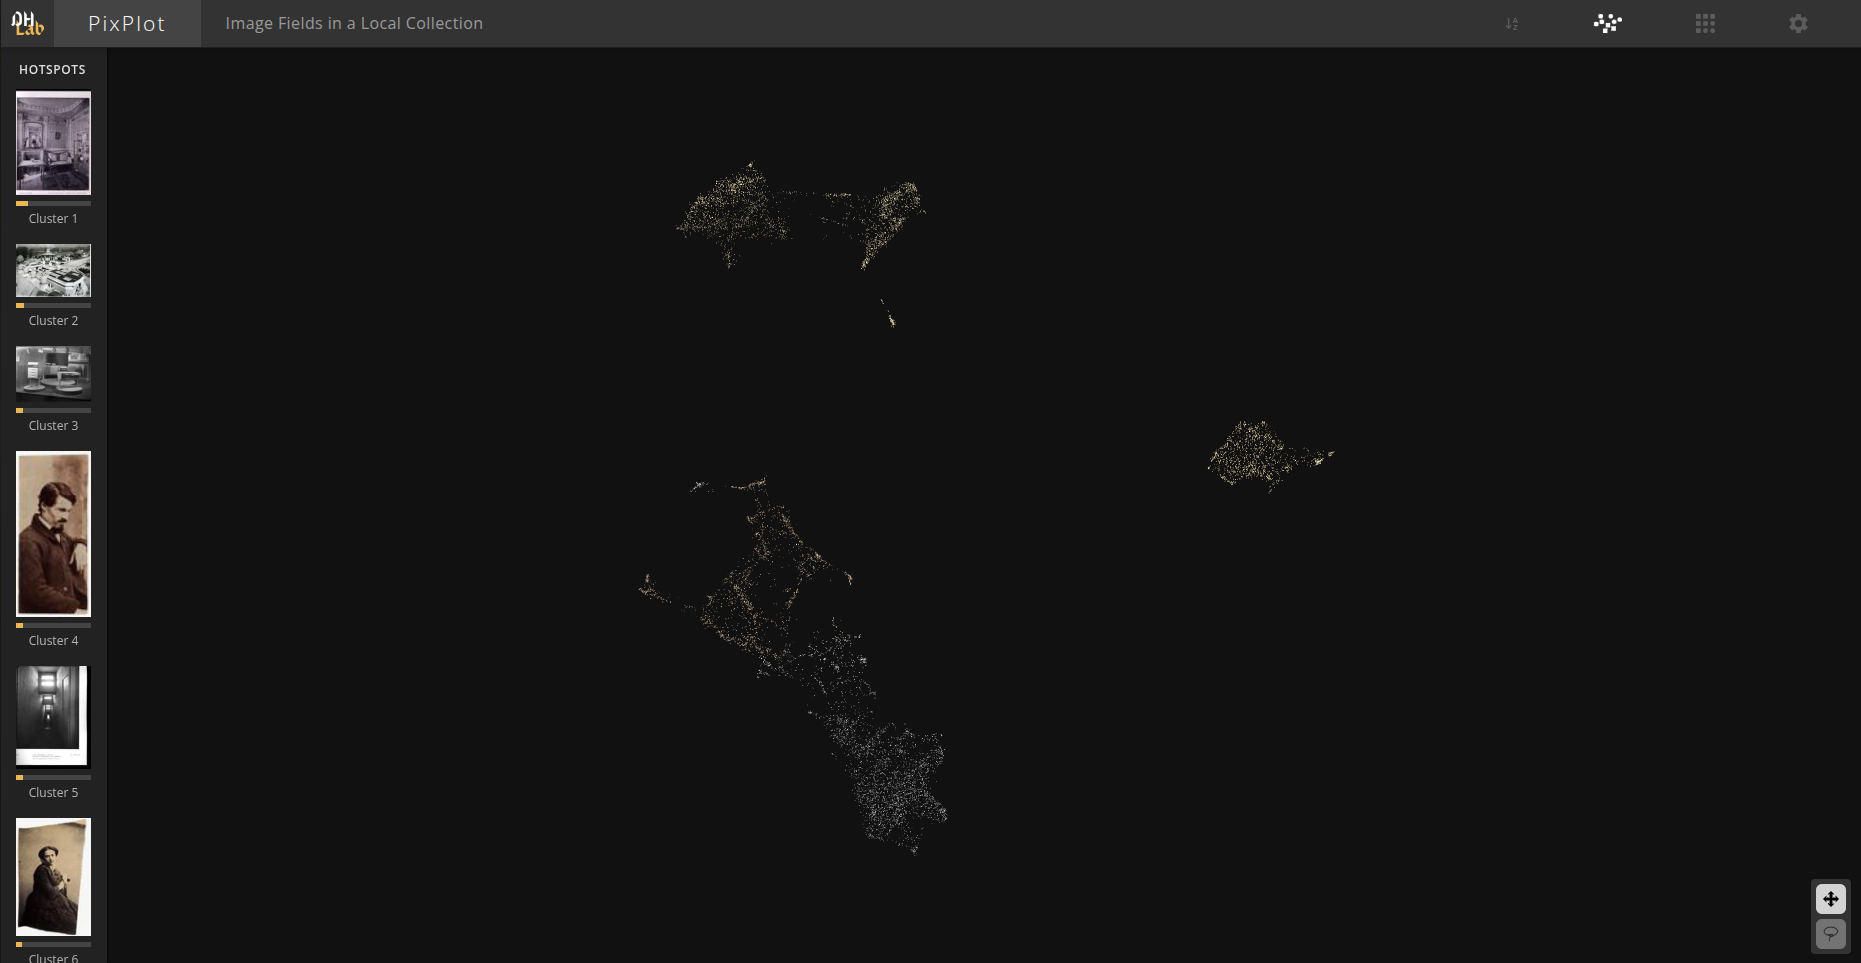
\includegraphics[width=\linewidth]{Illustrations/Pixplot2.png}
        \caption{}
    \end{subfigure}
    \begin{subfigure}{0.8\textwidth}
        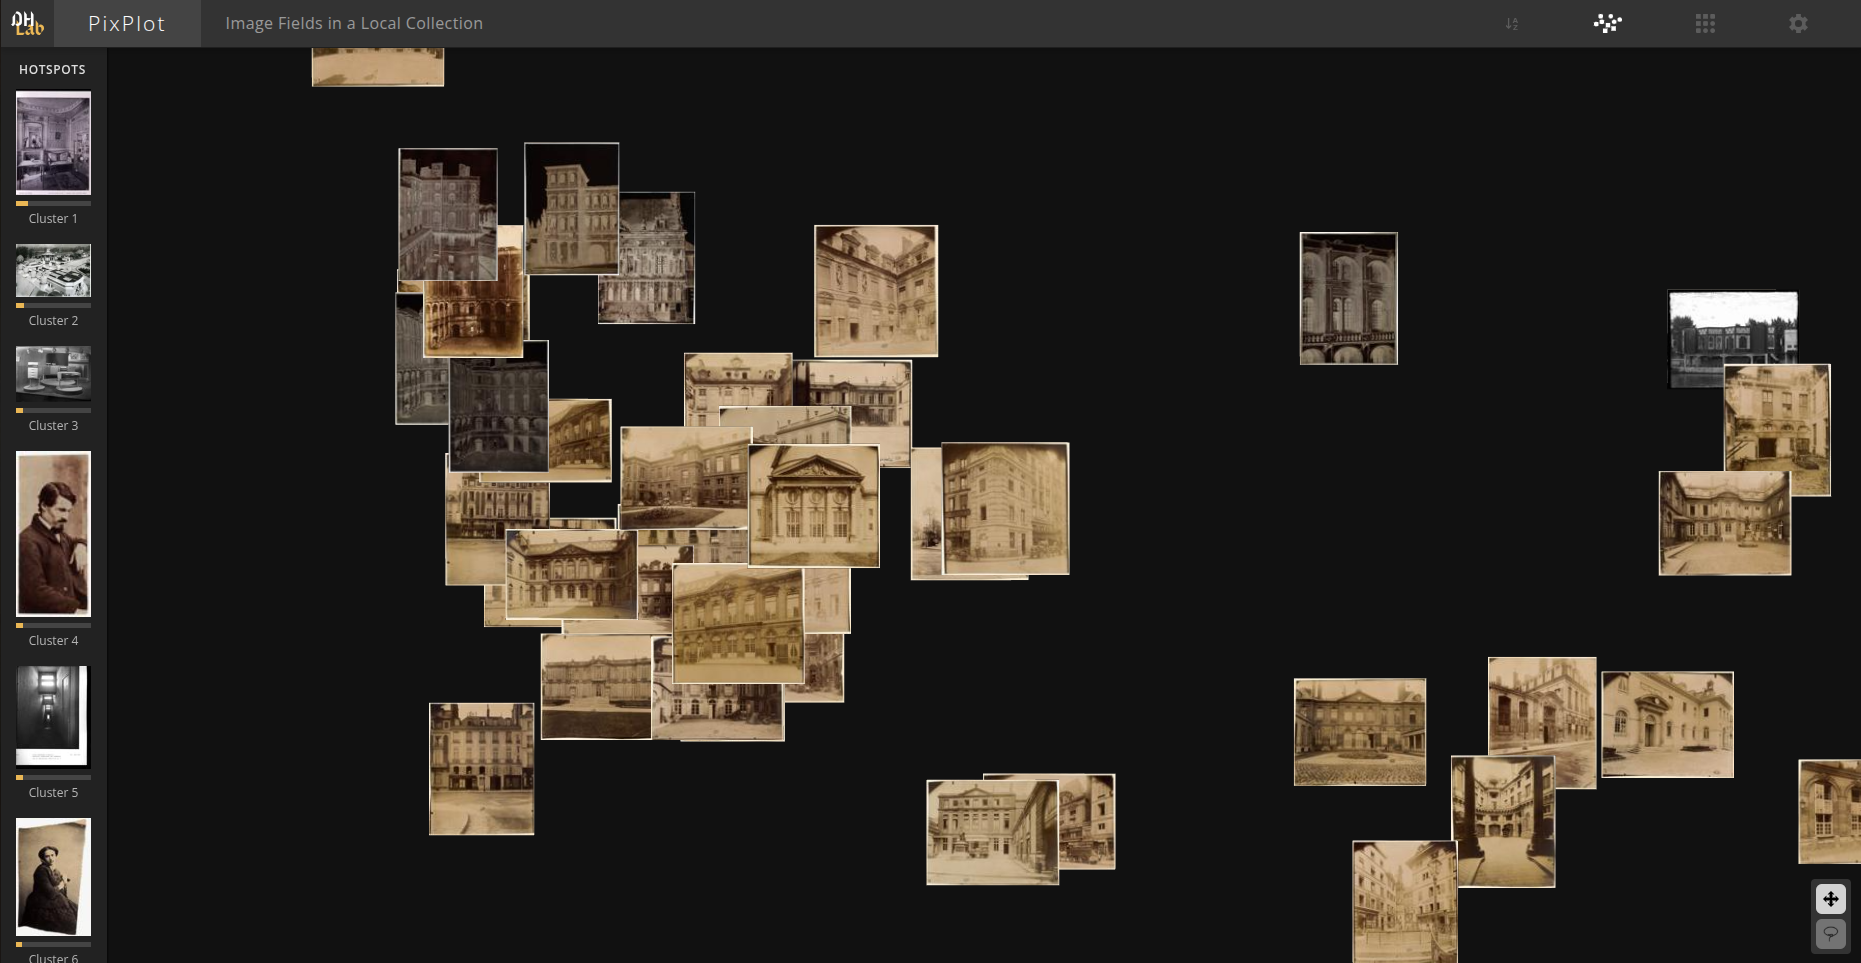
\includegraphics[width=\linewidth]{Illustrations/Pixplot3.png}
        \caption{}
    \end{subfigure}
    \caption{Illustrations de Pixplot}
    \label{fig:pellicules}
\end{figure}

Enfin, Pixplot qui est aussi un interface web et qui crée un carte en deux dimensions représentant les différences entre les images qu'on lui a fourni. C'est ce qui crée ces \enquote{continents} visuels qui rapproche les images des unes des autres ou les sépare en fonction de ce qu'elles représentent. Nous pouvons zoomer, retrouver les noms des fichiers et cliquer sur les images pour les agrandir. Cependant, l'application n'est pas reliée aux bases du musée, ce qui empêche d'avoir les chemins d'accès complet vers les dossiers où les images sont stockées.

\subsection{Le résultat des prises en main}

C'est donc l'utilisation de ces 3 outils-là que nous avons évalué au sein des équipes du département des Arts graphiques. La conduite des entretiens s'est déroulée entre juillet et août 2025 et ont tous fait l'objet d'une captation sonore et vidéo. Pour la transcription, nous avons eu recours à l'outil EchoInStone qui est un logiciel utilisant Whisper, logiciel de transcription développé par OpenAI, et qui ajoute une couche de diarisation au résultat\footnote{\cite{levy_jeanjeromeechoinstone_2025}}. Nous avons installé le logiciel sur le serveur JupyterHub du musée afin de pouvoir tirer profit des infrastructures, et spécifiquement du GPU du musée. Nous voulions la meilleure transcription possible donc nous avons lancé le modèle large pour chaque entretien, ce qui a demandé une puissance de calcul et un temps considérable qu'il n'aurait pas été possible de mobiliser avec notre ordinateur professionnel. 

Chaque outil remplit un rôle différent aux yeux des équipes et nous allons reprendre le résultat de ces prises en main ici. Nous avons, par ailleurs, produit une synthèse des entretiens qui se trouve en Annexe C\footnote{\textit{cf}. l'\textbf{\hyperref[sec:Annexe C]{Annexe C}}, p.~\pageref{sec:Entretiens_2025}.}. Tout d'abord \textit{Synesthesia} permet de raccourcir considérablement les temps de recherches dans l'inventaire et sur les bases du musée. Le cas d'usage le plus courant est celui où un\wokisme e chercheur\wokisme euse ou un particulier demande de retrouver un papier peint, un dessin ou une photographie dans les collections qu'il ou elle a pris en photo lors d'un passage au musée. Dans ce cas, l'outil est très pratique parce qu'il est relié autant à la base de données Arcadie du musée, qu'aux serveurs où se trouve l'ensemble de la production antérieure à la migration vers la base. Par similarité, l'outil retrouve l’œuvre dans les collections et indique combien il existe d'exemplaires de la même représentation d’œuvre, ses formats différents, ses emplacements. L'autre point soulevé lors des entretiens est l'aspect d'exploration que permet l'outil. En mettant une image de quelque chose de ressemblant, les personnels du musée peuvent aussi se laisser porter en explorant ce que l'outil trouve et être surpris, découvrir de nouvelles choses dans les collections, de nouvelles associations qui n'existent pas dans la base de données, etc,. Cependant l'outil reste limité en terme de cas d'usages à certains égards. En effet, la moitié des personnes sondées ne l'utilisent pas ou ne l'ont utilisé qu'une fois il y a longtemps. Les résultats peuvent s'avérer imprécis, l'outil produit du silence et l'instantanéité des résultats empêche paradoxalement l'exploration et la connaissance des fonds par tâtonnement. Aussi, l'outil met trop d'emphase sur les couleurs pour déterminer la similarité ou dissimilarité entre des images, là où, dans les cas d'usages, la question des motifs revient beaucoup plus souvent. Enfin, la recherche par texte est très peu utilisée et la recherche par métadonnées n'était pas connue des équipes. En général, l'outil est très utile pour les personnes qui s'en servent même s'il comporte des limitations.

Ensuite, en ce qui concerne Panoptic, la majorité des personnes interrogées s'est déclarée favorable à l'introduction de l'outil dans sa routine de travail. Les points en faveur de cette introduction qui sont ressortis après les manipulations sont les suivants : l'outil est rapide, il propose des regroupements indépendants d'un pré-traitement, il permet de guider la réflexion, de s'orienter dans un fonds mal connu, de requêter par texte, d'étiqueter les données et d'exporter ces étiquettes dans un csv avec les chemins de fichiers associés aux étiquettes, mais aussi de traiter les images en niveau de gris pour mitiger l'impact de la couleur sur les regroupements. Enfin, il permet de passer en revue une grande quantité d'image grâce à sa présentation sous forme de vignette et la facilité d'utilisation du zoom. Ce qui est ressorti est que pour caractériser un fonds défini, l'outil pourrait être très précieux, il est peut-être moins indiqué pour les recherches plus généralistes comme \textit{Synesthesia} en est capable. Quelques points négatifs ont été soulevés cependant, notamment certains regroupements hasardeux produits par l'outil qui ne semblaient pas faire sens pour le personnel, la possibilité de ne rechercher par texte qu'en anglais et le manque de compréhension des images. Ce dernier point vient du fait que l'outil a été pensé pour des images nativement numériques et non des photographies de supports ou d’œuvres. Ceci a pour effet de surdéterminer la similarité sur la base de la présentation physique des objets dans les photos (le même angle, la même lumière, la même table sur laquelle sont posées les œuvres) plutôt que sur le contenu, c'est-à-dire l’œuvre. Cependant, cette limitation peut être mitigée par la possibilité qu'offre l'outil d'y ajouter un plug-in avec par exemple un modèle Clip ré-entraîné qui se concentrerait plus sur les œuvres et moins sur le contexte des images. Dans l'ensemble, l'outil apparaît utile pour l'exploration et le traitement des collections, mais pas pour la médiation auprès d'un\wokisme e chercheur\wokisme euse ou du public.

Enfin, Pixplot semble être un outil intéressant pour la majorité des personnes sondées. Cependant, ils et elles précisent bien que c'est plus dans l'optique d'une première approche ou d'une visualisation très large d'un fonds qu'on ne connaît pas ou peu. Les personnes estiment que les rapprochements thématiques sont efficaces, bien que certaines anomalies et associations marginales dans les \enquote{continents} relèvent de l'erreur d'interprétation du modèle. Par exemple, les rapprochements des motifs de papiers peints étaient plus justes dans cet outil que dans Panoptic. La présentation de l'outil est esthétiquement agréable et intuitive, ce qui offre une belle première approche d'un fonds ou d'une collection de fonds. Il faut noter néanmoins, que l'impossibilité de retravailler les clusters après un premier résultat est très limitante. En général, pour l'exploration et la médiation des collections, l'outil est jugé adapté. En revanche, pour la description des collections, il ne convient pas.

\chapter*{Conclusion}

Cette partie se voulait être autant un compte-rendu du travail accompli, qu'un panorama de ce qui existe dans et autour du projet. Nous avons pu explorer la galaxie d'institutions et d'initiatives qui entourent l'entrée des humanités numériques utilisant l'IA dans les musées et le patrimoine. Nous avons aussi rendu compte des difficultés techniques, parfois organisationnelles, qui ont entourés les productions que nous avions à fournir. Nous avons pu aussi faire un premier bilan de l'introduction de l'IA au cœur d'un département de conservation. À notre sens, ce qui apparaît à l'aune de ces développements, c'est tout d'abord les opportunités et l'effervescence qui entourent ce domaine, mais aussi, en creux, l'autre face de ce genre de projets. En effet, si les opportunités sont nombreuses, les difficultés le sont tout autant. L'acculturation des équipes, les infrastructures, les limitations techniques, les spécificités des fonds, et bien d'autres domaines encore sont des points d'attention que nous devons garder à l'esprit face à la demande croissante de recours à ce genre de procédés. Depuis l'entrée de l'Intelligence Artificielle dans l'imaginaire du grand public, à la faveur de la sortie de ChatGPT le 30 novembre 2022, la notion d'IA exerce un formidable pouvoir d'attraction sur les individus comme les institutions, qui veulent s'emparer des nouvelles possibilités offertes par ces outils. Ce pouvoir d'attraction s'accompagne de réserves aussi, de la part de certain\wokisme e\wokisme s, mais aussi de certaines de confusions ou d'attentes démesurées vis-à-vis de l'outil. C'est tous ces points que se propose de traiter le prochain mouvement de ce travail, qui va s'attacher à pointer les limites, à souligner les opportunités et à proposer un certain nombre de manières d'introduire l'IA, de manière pérenne, au musée des Arts décoratifs, et plus largement dans les institutions patrimoniales françaises.	

%%%%%%%%%%%%%% PART 3 %%%%%%%%%%%%%%%%%%%%%%%%%%%%%%%%%%%
%%%%%%%%%%%%%%%%%%%%%%%%%%%%%%%%%%%%%%%%%%%%%%%%%%%%%%%%%

\part{Exigences scientifiques et pérennisation de l'IA}

%%%%%%%%%%%%%%%%%%%%%%%%%%%%%%%%%%%%%%%%%%%%%%%%%%%%%%%%%%%%%%%%%%%%%%%%%%%%%%%%%%%%
%%%%%%%%%%%%%%%%%%%%%%%%%%%%%%%%%%%%%%%%%%%%%%%%%%%%%%%%%%%%%%%%%%%%%%%%%%%%%%%%%%%%
%%%%%%%%%%%%%%%%%%%%%%%%%%%%%%%%%%%%%%CHAPITRE%%%%%%%%%%%%%%%%%%%%%%%%%%%%%%%%%%%%%%
%%%%%%%%%%%%%%%%%%%%%%%%%%%%%%%%%%%%%%%%%%%%%%%%%%%%%%%%%%%%%%%%%%%%%%%%%%%%%%%%%%%%
%%%%%%%%%%%%%%%%%%%%%%%%%%%%%%%%%%%%%%%%%%%%%%%%%%%%%%%%%%%%%%%%%%%%%%%%%%%%%%%%%%%%

\chapter{Familiarisation avec l'IA et limitations identifiées}

Au sein de cette partie nous voulons revenir sur le travail et les observations menées au sein même des équipes. Nous venons d'aborder le résultat des prises en main d'outils entre juillet et août 2025, mais le travail d'introduction et de formation à l'IA est un travail au long cours qui a été entamé dès le début de la collaboration entre le MAD et l'École des Chartes. 

\section{Enthousiasmes et réticences face à l'automatisation}

Dans le cadre des missions des musées labellisés "Musée de France", le musée des Arts décoratifs a pour mission de \enquote{Conserver, restaurer, étudier et enrichir [ses] collections}\footnote{\cite{noauthor_loi_2002}}. Cela implique entre autre la bonne tenue et documentation d'un inventaire des œuvres. Cette tâche, peut-être plus que celles concernées par l'automatisation, est souvent le point d'entrée par lequel les équipes abordent la perspective de l'introduction de l'IA dans leur travail. Nous allons donc détailler dans ce qui suit, le chemin parcouru et les éventuelles réticences soulevées par les employé\wokisme e\wokisme s au contact de l'IA.

\subsection{Le travail de pédagogie et de présentation}

Depuis le lancement du projet Royère il y a trois ans, un long travail d'expérimentation et de formation a été entamé au musée des Arts décoratifs, et pas seulement au département des Arts graphiques. Marion Charpier a formé les personnels et présenté des outils et des méthodes nouvelles à plusieurs équipes, tout en restant à l'écoute des besoins. Elle est notamment intervenue auprès du Service Informatique et de la gestionnaire de la base de données en plus du département des Arts graphiques. Ce travail de fond, d'acculturation des équipes et de vulgarisation de l'intelligence artificielle et de ses capacités à été crucial. En effet, tous les projets que nous pourrions formuler, ou qui pourraient être mis en place courent le risque de ne pas être utilisés ou de devenir accessoires, si les équipes ne s'en emparent pas. L'autre aspect est aussi que les agents ne doivent pas se sentir remplacés ou diminués par l'introduction de l'IA dans les processus de travail. C'est pourquoi le travail d'explicitation et de vulgarisation est primordial afin de montrer les limites et potentialités d'un outil d'IA.

Ces enjeux de présentation se sont poursuivis lors de notre présence au musée, que ce soit par la présentation que nous avons co-animée avec Marion Charpier et Emmanuelle Bermès face aux employés et à la direction le 24 avril 2025, ou bien par la campagne d'entretiens que nous avons menée, dans la droite lignée du travail entamé par Marion Charpier. En effet, deux ans après le début de la collaboration entre l'École des Chartes et le MAD, elle a mené une première campagne d'entretiens sur l'impact potentiel que pourrait avoir l'IA et son introduction au musée. Nous joignons ici ses conclusions et interrogations, avec ce que nous avons pu nous-même recueillir ou observer à propos des pratiques et conceptions autour de l'IA plusieurs mois après.

\subsection{Les leçons des entretiens et l'applicabilité de l'IA}

Dans la série d'entretiens menés en décembre 2024, plusieurs cas d'usages apparaissent. Il y a deux grands domaines dans lesquels l'introduction de l'IA pourrait être très utile : l'inventaire et l'exploration visuelle des collections. En ce qui concerne l'inventaire, l'IA pourrait faciliter l'indexation des œuvres et la gestion des archives historiques, en proposant des pré-indexations et de courtes descriptions sommaires afin d'attribuer des mots-clefs pertinents. Emmanuelle Bermès et Marion Charpier notent sur ce point :\enquote{Une autre possibilité réside aussi dans la création automatique de fiches d'inventaires, permettant d'attribuer systématiquement un numéro à chaque œuvre et de réduire le temps consacré aux tâches administratives}\footnote{\cite{bermes_repenser_2025}. p. 5.}. Pour les archives historiques, l'IA pourrait faciliter le traitement des numérisations et permettre l'amélioration des connaissances sur les œuvres, notamment en utilisant de l'HTR et du NER afin de croiser les informations et d'extraire les noms de personnes, lieux, organisations, etc,. mentionnés.

Pour l'exploration visuelle des collections, \enquote{l'IA pourrait considérablement enrichir l'exploration des collections en facilitant l'identification d’œuvres similaires, en optimisant la gestion des médias et en assistant les équipes dans leurs recherches de provenance}\footnote{\cite{bermes_repenser_2025}. p. 5.}. Il y a un vrai intérêt pour l'optimisation de la gestion des collections, mais cela implique plusieurs choses : \enquote{garantir la fiabilité des résultats, éviter les biais dans l'indexation, protéger la confidentialité des informations et s'assurer que les infrastructures techniques puissent supporter l'augmentation du volume de données traitées}\footnote{\cite{bermes_repenser_2025}. p. 5.}. En effet, la particularité des collections du MAD fait que beaucoup des œuvres présentes sont encore sous droits au profit de maisons ou de particuliers et que la libre diffusion de ces matériaux n'est pas possible. Il faut donc s'assurer que les traitements que nous mettons en place ne risquent pas de mettre entre les mains d'un tiers des données protégées ou sensibles. Un autre aspect qui ressort et qui invite à la prudence est le poids et le coût des numérisations. On estime que seul 30\% des collections sont numérisées, et bien que toutes les personnes que nous avons interrogées, pendant les entretiens de juillet-août 2025, citent que de nombreux fonds pourraient bénéficier de numérisations ou de traitements IA, toutes invitent à la prudence et préviennent que de trop grands volumes à traiter d'un coup seraient délétères pour la qualité et la faisabilité de leur travail quotidien. Enfin, la plupart des personnes disent être prêtes à consacrer du temps à la relecture ou correction de données générées, si cela permet d'aller plus vite que l'option manuelle, mais elles signalent aussi exiger une certaine qualité dans les données proposées. Tous\wokisme tes acceptent une marge d'erreur, tant qu'elle n'est pas inférieure à celle que pourrait faire un humain face à la même tâche, notamment pour les missions sensibles comme l'inventaire et l'indexation.

Afin de résumer, en reprenant la synthèse des entretiens de décembre 2024, le cadre d'application et l'impact de l'IA dessiné par les acteurs au fil des entretiens tient en cinq points fondamentaux. Il faut que l'IA soit appliquée dans un cadre sécurisé qui permette de garder le contrôle sur les enjeux de confidentialité et de contrôle des données sensibles. Il y a une grande motivation à appliquer l'IA afin de pouvoir traiter le volume important de passifs accumulés, que ce soit dans la base de données, l'inventaire ou la gestion des collections. L'utilisation de l'IA doit se faire dans un cadre strictement régulé, avec une tolérance partielle aux erreurs, des démarches de contrôle qualité par échantillonnage et des processus de validation sous la responsabilités des personnels scientifiques. L'absence de mise en œuvre de l'IA aurait pour conséquence de maintenir les délais actuels, parfois trop long, pour certaines tâches essentielles. Enfin, les erreurs produites par l'IA auraient un impact modéré, se traduisant principalement par des perturbations gérables dans le travail quotidien grâce à une supervision humaine régulière et à une attention particulière au volume de données générées pour ne pas submerger les personnels.

Parmi les personnes que nous avons pu interroger ou que Marion Charpier a interrogé, la plupart semblent enthousiaste à l'introduction de l'IA, mais il ne faut pas s'y tromper. Il y a bel et bien un intérêt et une volonté d'adopter l'IA au sein du musée, mais cet intérêt \enquote{repose avant tout sur la recherche d'une solution viable aux défis liés au traitement des collections. Plus que l'IA en tant que telle, c'est avant tout une réponse efficace au passif à traiter qui suscite l'intérêt des acteurs du musée}\footnote{\cite{bermes_repenser_2025}. p. 6.}. Il ne faut pas oublier non plus qu'il peut exister au sein du musée un ressentiment ou une crainte vis-à-vis de ce genre de projets. L'IA ne fait pas l'unanimité, certain\wokisme e\wokisme s redoutent d'être remplacé\wokisme e\wokisme s. Cela évoque des peurs, ou des griefs lorsque des budgets sont alloués à cela et pas à d'autres activités dans le musée, comme des restaurations ou des embauches. C'est en gardant tout cela à l'esprit que le déploiement d'un ou plusieurs projets IA doit se faire. 

Enfin, le grand absent de ces entretiens et expérimentations reste tout de même la photothèque du musée. Les projets Royère et TORNE-H s'articulant autour des collections d'arts graphiques, il est normal que l'attention se soit portée sur ce département. Cependant, au fur et à mesure de notre stage, il est apparu, de manière très claire, au gré des interactions informelles avec l'équipe de la photothèque, ou à travers certaines remarques des personnels de conservation du département des Arts graphiques, que l'équipe de la photothèque aurait aussi largement besoin d'outils pour faciliter leur travail. L'équipe a sous sa responsabilité toutes les ressources photographiques et numérisées du musée et semble effectivement être une cible de choix pour l'introduction d'outils de reconnaissance par similarité, ou de \textit{computer vision} pour leur permettre un traitement massif et structuré de ces données. 

\section{Des projets IA et des hommes}

Nous avons parlé de projets mobilisant l'IA, au sein des musées, des institutions patrimoniales ou d'entreprises, et nous mobilisons cette notion lorsque nous évoquons le projet Royère et TORNE-H, mais nous devons préciser deux distinctions fondamentales pour la suite de notre raisonnement. Tous les projets IA n'utilisent pas la même logique. Cela revient à ce que nous évoquions en Introduction lorsque nous distinguions entre IA connexionniste et IA symbolique, mais tous les projets IA n'utilisent pas les mêmes mécanismes. l'IA générative, la plus connue, celle des ChatGPT et autres agents conversationnels, se fonde sur les principes connexionnistes et offre une grande plasticité du fait de ses connaissances généralistes. Cependant, en dépit de sa facilité d'introduction dans un processus, de par l'absence de pré-configuration nécessaire, elle est celle qui rencontre le plus d'écueils dans des projets scientifiques, car sujette aux hallucinations et peu sûre en terme de confidentialité de données. De l'autre côté l'IA analytique génère des données structurées, est faite pour la catégorisation, la prédiction ou l'extraction de données et se base sur des algorithmes de machine learning pour accomplir sa tâche. Le projet TORNE-H, par exemple, se situe dans cette dernière catégorie. C'est la raison pour laquelle il est important de revenir sur quelques points d'attention et quelques exemples de projets passés ou présents qui peuvent nous en apprendre beaucoup sur les manières d'introduire ou non l'IA dans les domaines du patrimoine.

\subsection{Projets \textit{Venice Time Machine} et HikarIA}

Nous voulons vous présenter ici deux projets, l'un en cours, l'autre suspendu, afin de tenter de tirer les leçons de ces expériences dans le domaine patrimonial. Tout d'abord, un projet européen initié par l'université Ca'Foscari de Venise et l'École Polytechnique Fédérale de Lausanne (EPFL) en 2013 et concrétisé avec la signature d'un \textit{Memorandum Of Understanding} entre l'université, l'EPFL et les archives d'État de Venise en décembre 2014\footnote{\cite{castelvecchi_venice_2019}}. Le projet voulait reconstruire 1000 ans d'histoire de la cité à travers ses archives, leur numérisation et le recoupement avec les sources iconographiques et photographiques de la ville\footnote{\cite{epfl_presentation_2017}}. Le projet couplait HTR, NER, entraînement de modèle d'IA et numérisation massive des archives de la ville\footnote{\textit{cf}. le \textbf{\hyperref[sec:Glossaire]{Glossaire}} pour les termes \enquote{HTR} et \enquote{NER}, p.~\pageref{sec:Glossaire}.}. L'ambition était de mettre à disposition des historien\wokisme nes, des données massives et interrogeables afin de faire l'histoire sociale, politique et architecturale de Venise. Cependant, il semble que plusieurs problèmes aient mené à la suspension du projet, le 19 septembre 2019 par les archives d'État de Venise\footnote{\cite{noauthor_sospensione_nodate}}. Dans le communiqué, l'institution cite une absence de méthodes de travail uniforme, de norme de partage de données, une absence de communication entre les institutions, un manque d'équité, et une absence d'accord autour de la divulgation des données et des droits. En cinq ans, plus de 190 000 documents ont été numérisés, générant près de 8 TB de données\footnote{\cite{burns_venice_2019}}. Il semblerait que les deux problèmes principaux aient été les formats et l'absence de documentation idoine des numérisations qui auraient dû répondre aux exigences de la norme InterPARES utilisée par les archives d'État de Venise, et l'absence de communication entre les institutions\footnote{\cite{castelvecchi_venice_2019}}. Le second problème ayant causé le premier, les données générées se retrouvent inutilisables pour les archives en plus d'avoir été manipulées et gérées de manière opaque par l'EPFL. 

Ce que nous dit ce projet impressionnant mais malheureusement reporté \textit{sine die}, faute d'accord, est que dans les projets de numérisation et de traitement automatique la pleine transparence et maîtrise du processus par tous les acteurs est fondamentale. Pour notre cas ce ne sont pas plusieurs institutions étrangères qui doivent communiquer, mais l'incompréhension et le manque de transparence peut aussi très bien advenir entre des services ou entre une institution et un prestataire. C'est pour cette raison que le travail de pédagogie, de cadrage des besoins, d'explicitation des procédés, d'accord sur la forme des rendus finaux est primordial et doit être accompagné par des réunions de consultation et des points de passages concertés sur les projets, pouvant être inspirés des méthodes Agiles\footnote{\textit{cf}. le \textbf{\hyperref[sec:Glossaire]{Glossaire}}, p.~\pageref{sec:Glossaire}.}. 

Puis, le second projet, qui court jusqu'en 2026, est une collaboration entre l'entreprise Teklia et le musée Guimet à Paris. Il est soutenu par l’État dans le cadre du dispositif \enquote{Numérisation du patrimoine et de l’architecture} de France 2030, opéré par la Caisse des Dépôts\footnote{\cite{noauthor_projet_nodate}}. Le projet porté par Christopher Kermorvant, PDG de Teklia et Édouard de Saint-Ours, conservateur des collections photographiques au Musée Guimet a pour but d'entraîner \enquote{des algorithmes d’intelligence artificielle [...] à reconnaître des éléments visuels dans un vaste corpus produit entre le milieu du \textsc{xix}\textsuperscript{e}~siècle et le début du \textsc{xx}\textsuperscript{e}~siècle[...]. Ces algorithmes seront mis en œuvre sur une plateforme d’analyse qui feront émerger du corpus des données statistiques inédites sur les palettes de couleurs, les séquences d’images, les constantes et les ruptures iconographiques (doublons, lieux, décors, accessoires, modèles, typologies)}\footnote{\cite{noauthor_projet_nodate}}. Il y a deux volets au projet, une partie découpage automatisé des images dans les albums avec un entraînement de modèle d'extraction de photographie, qui semble avoir donné des résultats très satisfaisants. Le résultat de ces extractions sont les nombreuses vues disponibles sur le site du projet\footnote{\cite{noauthor_hikaria_nodate-1}}. De plus, la présentation des vues propose un système de \textit{clustering} par similarité, très proche des technologies que nous avons expérimentées dans le stage, qui propose des images que l'algorithme juge similaires à celle que nous regardons en bas de page.

L'autre volet, qui semble avoir été abandonné depuis la version 0.2.6 du projet, mais qui était encore présent dans la version 0.2.5, était la génération de mots-clefs et de descriptions automatiques par un LLM afin d'enrichir les métadonnées et les descriptions. En effet, quand nous avions inspecté les résultats générés sur la dixième vue de l'album 47 du fonds Dubois, on pouvait voir tant des mots-clefs établis par le documentaliste que ceux générés par IA\footnote{\cite{noauthor_hikaria_nodate}}. La photographie montre deux femmes portant des ombrelles devant un portail en bois menant à une maison. Si le grand modèle de langue avait relevé quelques termes pertinents non indexés par le documentaliste, notamment \enquote{barrière}, \enquote{portail} ou \enquote{chemin}, beaucoup de termes générés sont faux ou non pertinents, comme \enquote{bac à gaz}, \enquote{punition}, \enquote{consulat} ou, de manière plus problématique, \enquote{Chine}. Depuis, ces descriptions automatiques ont été enlevées du site et notre seule source est le travail de rédaction de Pierre Husson dans le cadre de son stage à l'INHA, qui a rédigé une partie sur le projet avant sa mise à jour, fin août, et qui nous permet de sourcer ce que nous avions vu à l'époque sans le prendre en capture d'écran ou l'archiver. 

On comprend néanmoins pourquoi ce volet du projet, pourtant si prometteur, a été retiré (peut-être seulement temporairement). Du point de vue d'un conservateur, des photographies japonaises du \textsc{xix}\textsuperscript{e}~siècle, qui se retrouvent affublées d'une description \enquote{Chine} est intolérable, et à raison . L'ancrage culturel des modèles d'IA dans des perspectives culturelles occidentales, explique l'erreur : les données d'entraînement comprennent des biais culturels, qui sont reproduits dans les analyses produites. Le projet a encore un an devant lui, et il est doté d'un corpus numériquement similaire au nôtre avec le projet Royère (environ 18 000 photos). Beaucoup de choses peuvent encore changer, et être affinées mais il nous semble que cela nous invite à deux constats importants pour nous. D'abord, la notion de marge d'erreur ne comprend pas du tout les mêmes types de problèmes que lorsque l'on parle de marge d'erreur dans le travail humain de récolement et de description. Dans les entretiens menés par Marion Charpier, il apparaît que les personnels sont prêts à accepter une certaine marge d'erreur, en vertu de la probabilité similaire qu'il existe des erreurs dans le travail humain. Cependant, du point de vue scientifique, le type d'erreur que peut générer un traitement automatisé n'est pas du tout de même nature qu'un oubli ou une erreur d'interprétation, qui elles auront toujours bien plus le contexte à l'esprit. Un LLM malheureusement est aussi emprunt de biais, tout comme les humains qui l'ont construit ou les données sur lesquelles il a été entraîné. Ce qui nous fait arriver à notre second constat : la méfiance nécessaire vis-à-vis des données générées par une IA générative de type Chat-GPT, Claude, Mistral, Deepseek, etc,. Ces modèles sont par nature des modèles probabilistes, ils génèrent en fonction de la plus ou moins haute probabilité que le mot \textit{N} suive le mot \textit{N-1} et fasse sens dans le contexte qu'il comprend via ses embeddings\footnote{\textit{cf}. le \textbf{\hyperref[sec:Glossaire]{Glossaire}}, p.~\pageref{sec:Glossaire}.}. La nature généraliste et biaisée de ces modèles invite donc à la plus grande méfiance et retenue dans leur utilisation pour des collections patrimoniales, imposant, par exemple, l'utilisation d'un vocabulaire contrôlé ou d'une ontologie fixe pour les générations, un peu à la manière de l'inférence Royère.

\subsection{Points d'attentions et moyens humains}

Dans ces projets et dans d'autres qui pourraient exister au sein du musée des Arts décoratifs ou ailleurs, il est crucial de garder à l'esprit deux choses pour la pérennité des résultats des traitements automatisés : les cas d'usages et le coût humain de la numérisation ou de l'automatisation. Le premier point est d'autant plus crucial que \enquote{réussir un projet IA, c’est avant tout répondre aux besoins des équipes terrain. Ce qui signifie, identifier avec précision l’usage futur de l’IA au sein de l’organisation afin de définir des choix technologiques, de structurer l’allocation de ressources et de s’atteler à un sujet conséquent : la préparation des données}\footnote{\cite{it_social_ia_2025}}. Nous prenons cette citation d'un magazine technologique destiné aux entreprises et qui parle des entreprises, mais il nous semble cependant qu'une partie des conclusions qu'ils tirent sur l'introduction de l'IA en entreprise, soient applicables dans notre cas. En effet, l'article cite le taux d'échec élevé des projets IA en entreprise (85\%), et bien que nous soyons bien incapables de donner une statistique similaire dans le milieu du patrimoine et des humanités numériques, il n'empêche que les raisons évoquées sont éloquentes à plusieurs égards : 
\vspace{1em}

\noindent
\hspace*{1cm}
\begin{minipage}{\dimexpr\linewidth-2cm}
\fontsize{10}{12}\selectfont
Les entreprises manquent fondamentalement d’expérience et de recul[...] Un des premiers indices de cette non-maturité est structurel. Sans expérience ni méthode, un grand nombre d’entreprises tendent à créer des couches organisationnelles redondantes. Il est ainsi fréquent de voir émerger des départements spécialisés IA en supplément de départements existants dédié à l’innovation ou à l’informatique.\footnotemark{}
\end{minipage}

\vspace{1em}

\footnotetext{{\cite{it_social_ia_2025}}} 

Le second point fait référence à l'effort consenti et conscientisé par l'institution pour intégrer durablement les données ou numérisations produites. Dans le cas des numérisations, le problème n'est pas nouveau, mais il fonctionne de manière similaire. 


\vspace{1em}

\noindent
\hspace*{1cm}
\begin{minipage}{\dimexpr\linewidth-2cm}
\fontsize{10}{12}\selectfont
De nombreux projets de numérisations, ont fleuri il y a quelques années, à la faveur de financements en ce sens. Nous nous sommes retrouvés avec quantité d'images, qui sont restées là sur des disques dur ou des drives, dont on a perdu la trace ou qui n'ont pas survécu au passage dans la base de donnée commune des musées en 2015. Certes, certaines campagnes de numérisations sont redécouvertes par la suite, mais la plupart du temps, nous les responsables des collections, n'avons pas le temps d'accomplir ce travail de fond de caractérisation et d'intégration, pourtant nécessaire. \footnotemark{}
\end{minipage}

\vspace{1em}

\footnotetext{Propos recueillis auprès de Sébastien Quéquet, attaché de conservation en charge des collections de photographie au MAD, le 12 août 2025.} 

Le point sur lequel appuyait Sébastien Quéquet lors de notre entretien est celui du manque de main-d’œuvre pour absorber et intégrer durablement, notamment dans la base Arcadie, les informations et les représentations des œuvres. Il cite évidemment l'embauche de stagiaires ou de contrats courts pour réaliser cette tâche, mais cela peut s'avérer compliqué lorsque l'on sait que les postes ponctuels comme ceux-là, sont conditionnés le plus souvent à l'obtention d'un mécénat. C'est pour cela qu'il évoquait la nécessité de penser en amont, dans la création et le financement d'un projet, à l'embauche des personnes qui pourraient faire ces intégrations. 

Une autre piste évoquée à ce moment-là, et qui est déjà fort répandue dans le monde des archives, est l'indexation collaborative. Il s'agit de campagnes ouvertes au publics, organisées par les archives départementales de nombreuses localités, qui ont pour but de mettre à disposition des numérisations d'archives, d'une même source (par exemple archives ecclésiastiques ou notariales) et de les faire annoter par les érudits locaux et les passionnés d'histoire de la région afin de faciliter le travail des archivistes. La plateforme qui réunit ces initiatives pour les Archives Nationales se nomme Girophares et a été lancée en 2023\footnote{\cite{noauthor_archives_nodate}}. Il existe aussi de nombreuses archives départementales comme celles de Haute-Garonne, du Calvados, du Bas-Rhin, de l'Oise, du Cantal et bien d'autres qui disposent d'interfaces similaires. Ce qui nous fait dire que l'option n'est pas si fantasque, est qu'un premier essai en musée a déjà eu lieu au Musée de Bretagne\footnote{\cite{noauthor_lindexation_nodate}}. En 2020, accompagné par la Bnf, la société Teklia, la société Decalog et dans le cadre d’un appel à projet à services numériques innovants, lancé par le ministère de la Culture, le musée lance sa plateforme pour indexer ses fonds photographiques.

Ce qu'il s'agit ici de démontrer est que le besoin doit toujours présider au développement d'une solution. Cette solution doit s'intégrer dans les habitudes et le travail des équipes, sans causer de doublons ou de redondances organisationnelles. Les possibilités de l'IA peuvent effectivement déclencher un effet d'attraction, mais il faut toujours réfléchir en amont aux résultats attendus ou recherchés et à la mise en place d'un environnement de données adéquat\footnote{À cet effet le guide produit par la \textit{Library of Congress} nous semble très éclairant à plusieurs égards : \cite{manchester_introducing_2023}}. Enfin, les logiques de projet doivent inclure dans leur calendrier et leur budget les moyens de la pérennisation de ces productions, que ce soit par des équipes de suivis ou le personnel scientifique nécessaire à la pleine intégration des informations dans les corpus du musée.

%%%%%%%%%%%%%%%%%%%%%%%%%%%%%%%%%%%%%%%%%%%%%%%%%%%%%%%%%%%%%%%%%%%%%%%%%%%%%%%%%%%%
%%%%%%%%%%%%%%%%%%%%%%%%%%%%%%%%%%%%%%%%%%%%%%%%%%%%%%%%%%%%%%%%%%%%%%%%%%%%%%%%%%%%
%%%%%%%%%%%%%%%%%%%%%%%%%%%%%%%%%%%%%%CHAPITRE%%%%%%%%%%%%%%%%%%%%%%%%%%%%%%%%%%%%%%
%%%%%%%%%%%%%%%%%%%%%%%%%%%%%%%%%%%%%%%%%%%%%%%%%%%%%%%%%%%%%%%%%%%%%%%%%%%%%%%%%%%%
%%%%%%%%%%%%%%%%%%%%%%%%%%%%%%%%%%%%%%%%%%%%%%%%%%%%%%%%%%%%%%%%%%%%%%%%%%%%%%%%%%%%

\chapter{La \textit{computer vision} au musée en puissance et en acte}	

Fort des connaissances sur les possibilités offertes par la recherche actuelle en humanités numériques, et conscient de l'histoire et de la particularité du musée des Arts décoratifs et de l'Union Centrale plus largement, nous nous proposons de dresser un premier bilan et un premier tableau prospectif de l'introduction de l'IA dans l'institution.

\section{MLOps et compétences techniques nécessaires}

L'un des enjeux du projet Royère puis du projet TORNE-H, était la formation des équipes aux notions fondamentales de l'IA. L'un des aspects de cette formation que nous n'avons pas encore évoqué était celle à destination du Service Informatique du musée. En effet, de par leur rôle, tout projet d'automatisation ou de \textit{Machine learning} devait aussi être réfléchi avec le service pour qu'il puisse être mis en place. C’est pourquoi Marion Charpier a assuré un certain nombre de formations sur les fondamentaux de l'IA et de son environnement auprès du SI. Les équipes du SI, curieuses d'apprendre, se sont prêtées au jeu et ont fait tout ce qui était en leur pouvoir afin de mettre en place un environnement de développement, comme nous l'évoquions dans une partie précédente. Elles ont aussi participé aux discussions autour de la conception des flux de données et ont veillés à la sécurisation des matériaux dans le cadre du projet Royère. 

Dans ce cadre, plusieurs journées de bilan, formation et ateliers ont eu lieu pendant le stage. S'est tenu un atelier de cartographie des compétences nécessaires pour la mise en place d'une opération de \textit{Machine learning}. Une intervention de la part de la Fondation SAHAR, dans le cadre d'un mécénat de compétences, pour nous introduire au DevOps et au rôle d'un \textit{Data Scientist}, et enfin une formation à Docker et à la conteneurisation d'application par un enseignant de l'École\footnote{\textit{cf}. le \textbf{\hyperref[sec:Glossaire]{Glossaire}} pour le terme \enquote{\textit{Data Scientist}}, p.~\pageref{sec:Glossaire}.}. Ces initiatives ont permis de mettre en lumière le chemin qu'il restait à parcourir avant la mise en production pérenne d'une opération de \textit{Machine learning}, mais aussi la capacité d'adaptation et la volonté d'apprendre des équipes du musée.

\subsection{Décrire une chaîne IA}

Afin de bien comprendre de quoi il retourne lorsque nous parlons de la mise en production d'une opération de \textit{Machine learning}, nous revenons ici très généralement sur la manière dont se construit une chaîne de production MLOps, puis plus précisément sur son applicabilité dans le domaine patrimonial. Nous nous appuyons sur un article de recherche généraliste et orienté vers l'application d'un MLOps dans le secteur privé pour donner un aperçu des grandes questions et enjeux qui parcourent l'élaboration et la mise en production d'un projet de \textit{machine learning}\footnote{\cite{kreuzberger_machine_2023}}. 

\begin{figure}[H]
    \centering
    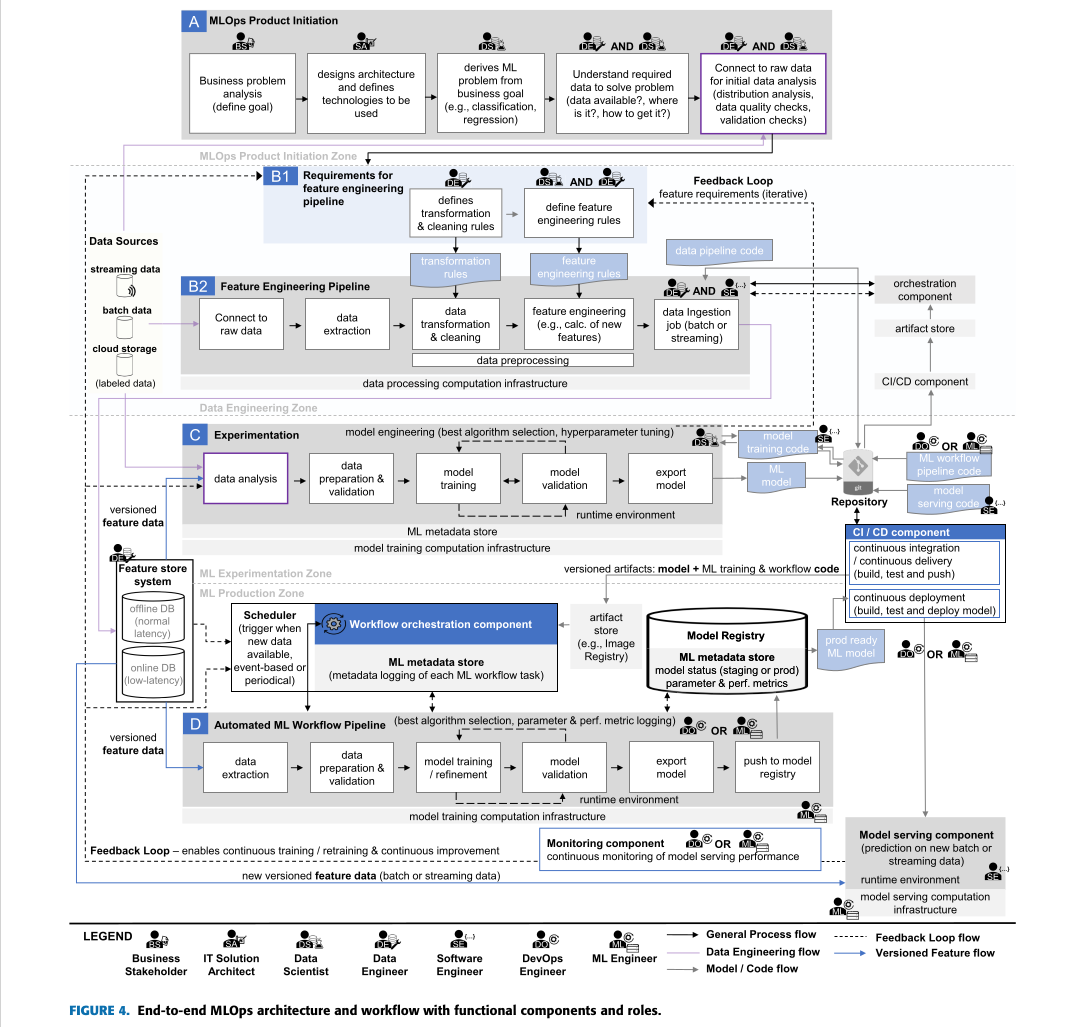
\includegraphics[width=1.08\linewidth]{Illustrations/MLOps.png}
    \caption{Schéma d'une architecture de MLOps}
    \label{fig:placeholder}
\end{figure}

Si nous reprenons le modèle exposé dans ce schéma, très complet et complexe, on voit plusieurs choses\footnote{\cite{kreuzberger_machine_2023}. p. 31873}. Il comprend quatre grandes étapes : l'initiation du projet, la conception des \textit{features}, l'expérimentation et la mise en production. Ce que nous devons garder à l'esprit est la diversité des compétences requises pour mener à bien un tel processus. Entre les personnes métiers qui prennent part au processus, les ingénieurs logiciel, DevOps, \textit{Data} et \textit{Machine learning}, un \textit{Data Scientist}, un \textit{Data engineer} et un \textit{IT Solution Architect}, beaucoup de corps de métiers entrelacés sont convoqués. Dans l'exemple donné, le schéma est appliqué à un produit commercialisable, et dans les ambitions d'un musée, une équipe aussi nombreuse ne serait sans doute pas pertinente. Cela demande tout de même que les personnes aient des compétences hybrides et transversales et qu'une certaine expérience de l'industrialisation et de la gestion de flux de données soit présente.

Aussi, il faut garder à l'esprit que l'histoire de l'art se prête assez mal aux traitements quantitatifs. C'est la raison pour laquelle Marion Charpier a dû utiliser un algorithme de déformation d'images pour enrichir le jeu de données dans son \textit{workflow} TiamaT.

\vspace{1em}
\noindent
\hspace*{1cm}
\begin{minipage}{\dimexpr\linewidth-2cm}
\fontsize{10}{12}\selectfont
While museum datasets are not complete enough to train algorithms potentially museums could work together to produce an algorithm that could be applied in the sector. There is also an opportunity for museums to partner with the data science community to create machine learning models based on smaller datasets specifically for art objects.                                                  \footnotemark{}
\end{minipage}
\vspace{1em}
\footnotetext{\cite{murphy_museum_2020}. p. 9.}

Ce sont toutes ces questions qui ont mené le projet TORNE-H à s'orienter vers une démarche résolument qualitative en privilégiant l'apprentissage supervisé à l'apprentissage machine. Nous voulons partager un extrait d'un livre collectif publié en 2010, qui illustre assez bien les questions qui se posent aujourd'hui en histoire de l'art et traitement patrimonial en lien avec l'IA : 

\vspace{1em}
\noindent
\hspace*{1cm}
\begin{minipage}{\dimexpr\linewidth-2cm}
\fontsize{10}{12}\selectfont
Pourquoi les statistiques, les graphiques et les cartes ne sont-ils pas aimés en histoire de l’art ? Les approches quantitatives dans ce domaine, souvent importées de la sociologie, portent probablement la macule de la discipline de Durkheim : réductionnisme, incapacité à rendre compte des œuvres, approche centrée sur les stratégies, le marché, l’argent, le collectif et la norme, alors que l’art et la création sont inséparables du désintéressement, des sacrifices, de l’individualité, du génie, et que le rôle de l’historien de l’art est de reconstituer des styles, de rendre compte de la valeur de l’art et des œuvres exceptionnelles.                                                \footnotemark{}
\end{minipage}
\vspace{1em}
\footnotetext{\cite{joyeux-prunel_lart_2010}. p. 17.}

Tout cela a été écrit en 2010, plusieurs années avant l'émergence des première réflexions autour de l'intelligence artificielle et de l'histoire de l'art. Cela n'empêche pas que, pour nous, nous retrouvions les mêmes problématiques, les mêmes tensions entre sciences idiographiques et sciences nomothétiques, que celles qui ont traversé les réflexions en histoire et sociologie par rapport à l'émergence au \textsc{xx}\textsuperscript{e}~siècle du quantitativisme. Les démarches statistiques fondées sur les grands ensembles de données et la répétition, qui sont l'apanage des modèles d'intelligence artificielle, ne sont pas toujours compatibles avec la particularité des fonds ou la singularité des oeuvres. C'est cette tension que l'on doit aussi garder à l'esprit pendant l'élaboration d'un projet de \textit{machine learning} dans une institution patrimoniale. En d'autres termes : que peut-on attendre, ou que ne faut-il pas attendre d'un traitement par IA sur des collections patrimoniales ?

\subsection{Le traitement Royère et le projet TORNE-H}

La tentative d'introduction d'un processus de \textit{machine learning} nous a permis de cadrer les besoins et d'explorer les possibilités et limites de cette démarche. Avant l'opérationnalisation d'un traitement IA, plusieurs étapes sont fondamentales. Nous l'avons déjà détaillé : le recueil des besoins, l'étude de l'état des données, des collections et de l'infrastructure existantes, le diagnostic des compétences et la marge d'évolution possible des personnels et infrastructures. Toutes ces composantes interviennent avant même le traitement IA à proprement parler. Pour ce qu'il en est du processus en lui-même, et de ce que nous pouvons généraliser à partir de ces deux projets, Royère et TORNE-H, nous pouvons dire deux choses. D'abord il y a un intérêt réel, tant du point de vue scientifique, que du point de vue des équipes, pour l'introduction de ce genre de traitement, et les bons résultats de l'inférence Royère nous font dire que la démarche de \textit{fine-tuning} porte ses fruits et est pleinement justifiée dans le cadre des collections patrimoniales. Cependant, nous avons du mal à amener la précision et le détail d'analyse que les équipes souhaiteraient. Nous avons pu caractériser ce qu'il se trouvait sur les 12 000 images, mais pas les motifs ou les modèles de meubles, ce qui aurait vraiment été une valeur ajoutée pour les personnels en charge des collections. Ensuite, outre les limitations techniques de puissance de calcul, la base de données Arcadie n'est pas en mesure d'absorber de grandes quantités de notices à la fois sans risque de crash. Nous sommes limités à des lots de 10 GB de médias à la fois et quand il s'agit d'une collection de 12 000 images, cela peut s'avérer très compliqué. La tâche est d'autant plus complexe que les imports doivent se faire sur les heures de travail et au prix d'un ralentissement de la base pour tous les autres utilisateurs\wokisme trices. Il n'existe aucun moyen de faire des imports la nuit ou le week-end, sans parler de l'absence d'API qui empêche de massivement importer des notices et des médias et qui force à passer par une interface web peu ergonomique. 

Le résultat du projet est très encourageant, en inversant le processus et en caractérisant d'abord les objets des collections avant de les faire relire par les personnels scientifiques, on permet qu'une quantité d'informations et de métadonnées soient déjà produites. Quand bien même ces métadonnées sont sujettes à caution, avec un marquage spécifique dans la base afin d'indiquer que les informations ont été générées, cela permet tout de même d'enrichir les possibilités d'interrogation de la base pour les personnels du musée. Aussi, les technologies de reconnaissance généralistes semblent montrer leurs limites dans un contexte d'histoire de l'art, et une approche plus qualitative semble plus indiquée pour le traitement des collections. Ce point demande donc d'arbitrer entre les projets, les fonds qui seront traités de cette manière, et ceux qu'il reste à numériser. En effet, il faut rappeler qu'on estime que seulement 30\% des collections sont numérisées et ces enjeux de numérisation représentent un défi concret pour l'introduction massive de l'IA au musée. Enfin, en dépit de la maturité avancée de l'institution dans sa réflexion sur sa stratégie numérique, on voit que certaines barrières et certains freins présentent encore des limites très concrètes à la faisabilité et l'intégration efficace des résultats d'un procédé de \textit{computer vision} au musée.

\section{Scenarii d’intégrations de l'IA}

Conscients des caractéristiques, enjeux et limitations de la mise en application de l'IA dans le domaine patrimonial, nous proposons dans cette dernière section un regard au présent et au futur sur l'intégration de l'IA au musée. Nous parlerons du contexte institutionnel et politique particulier et particulièrement favorable à ce genre d'initiatives, et des précautions que ce genre d'enthousiasme implique. Nous parlerons aussi des trois scenarii types de l'introduction de l'IA et de sa gestion dans le cadre actuel. 

\subsection{Le contexte institutionnel}

On se tourne à nouveau vers l'histoire de l'institution, et le rôle qu'elle a joué comme précurseur de l'établissement des arts décoratifs dans le paysage artistique français. Nous pouvons noter aussi sa mission patrimoniale particulière et le caractère unique de ses collections, avec notamment son musée de l'affiche et de la publicité, ou son musée du jouet. Ou bien encore sa contribution à ce qui allait devenir le Centre Pompidou avec la création du Centre de Création Industrielle (CCI) et sa fusion avec le Musée national d'Arts Moderne (MNAM) en 1992\footnote{\cite{caroll_centre_nodate}.}. Tout cela montre bien comment l'innovation est au cœur du projet de l'UCAD, et comment cette institution si particulière s'est créée sa place au sein du paysage muséal français, en explorant de nouveaux champs pour en faire des objets d'Histoire, d'étude et de préservation. Nous pouvons comprendre, dans la lignée de ce souffle, l'intérêt aussi pour les nouvelles opportunités qu'offre l'IA, qui en plus des usages que nous pouvons en faire pour le traitement des collections, représentent encore un nouveau champ à défricher et dont l'institution peut se saisir.

L'année 2025 présente un contexte favorable à l'introduction durable de l'IA dans l'écosystème patrimonial français à plusieurs égards. Premièrement, pour le musée, l'obtention pour la deuxième année de suite d'un financement du Fonds d’accompagnement à la transformation numérique et à la cybersécurité des établissements du ministère de la Culture (FTNC), assure les moyens de ces ambitions. Ensuite, la présence à temps partiel de l'ingénieur Robert Erdmann pour la mise en place d'outils utilisant l'IA pour automatiser les manipulations avec la base de données et pour aider les équipes dans le cadre de l'application \textit{Synesthesia} représente une opportunité très intéressante pour le musée. Enfin, l'annonce en fin juillet, par la Ministre de la Culture, Rachida Dati, d'un partenariat entre le Ministère et Microsoft pour l'introduction de l'IA à des fins de valorisation et de promotion du patrimoine français, représente une occasion exceptionnelle pour le musée, qui fait partie des institutions bénéficiaires du partenariat\footnote{\cite{noauthor_discours_2025}.}. Plus largement, l'année 2025 a été marquée par plusieurs annonces et discours du Président de la République, Emmanuelle Macron, à l'occasion du \enquote{Sommet pour l'action sur l'IA}, co-organisé par la France et l'Inde, et qui s'est tenu les 10 et 11 février au Grand Palais à Paris. La veille, dans une interview sur France 2, le président annonce plus de 109 milliards d'euros d'investissement dans le domaine de l'IA\footnote{\cite{noauthor_replay_2025}.}. Le lendemain, il annonce la mise en chantiers de \textit{Data centres}\footnote{\textit{cf}. le \textbf{\hyperref[sec:Glossaire]{Glossaire}}, p.~\pageref{sec:Glossaire}.} sur le territoire, et dit vouloir mettre \enquote{l'IA au service de l'humanité}\footnote{\cite{noauthor_prononce_2025}.}. 

Outre ces effets d'annonce, et si l'on garde à l'esprit que tous ces investissements n'iront pas uniquement pour la culture, il n'empêche que le moment apparaît propice à l'expérimentation et à la mise en place, à grande échelle, de chaînes de traitements IA dans les musées et institutions patrimoniales françaises. Le pouvoir de traction, et l'engouement politique autour du sujet assure, au moins pour le futur proche, un soutien financier pour ce genre d'initiatives. En revanche, il ne faut pas oublier un point que nous avons déjà soulevé par ailleurs, c'est-à-dire la précaution qui est aussi de mise dans ce genre de projets, et d'autant plus s'ils font l’objet de tels enjeux politiques. Il est primordial que les projets répondent à des besoins et s'inscrivent dans la durée au sein des institutions, au risque d'assister à une débauche de moyens pour des projets attractifs en théorie et qui finiraient par être inopérants ou peu adaptés. Pour cela, les démarches patientes d'approche des besoins, de compréhension des enjeux métiers et de la spécificité des institutions et de leur passif sont primordiales. 

Enfin, et il est important de le noter, il faut rappeler que ces projets, l'IA, les \textit{Data centres}, et les autres ressources nécessaires à la conduite et à l'opérationnalisation de processus automatisés à grande échelle, ont un coût environnemental énorme. Si les institutions patrimoniales françaises ont pour vocation de léguer aux générations futures, l'histoire, l'art, la richesse et la culture de ceux qui les ont précédés, il est, il nous semble, aussi de leur devoir de veiller à le faire de la manière la plus consciente et frugale possible. Ce dernier point va de pair avec une approche patiente et raisonnée de l'introduction de l'IA dans le paysage muséal français.

\subsection{L'arbitrage entre compétences internes et prestations}

Dans ce contexte, trois grandes voies s'offrent au musée en vue de l'intégration durable de processus IA dans son traitement des collections et ses routines de travail. La première consiste à externaliser tout le traitement et le processus auprès d'un tiers ou d'un entreprise privée, à qui on confie un cahier des charges et qui est chargé de produire les résultats dont les personnels ont besoins dans leur gestion quotidienne des collections. Cette option implique plus de flexibilité, mais aux dépens du contrôle et de la souveraineté de l'institution sur les processus et les traitements de données, qui resteront toujours opaques en l'absence d'agents interne au musée dans le processus. L'autre risque est la perte des outils et logiciels développés par le tiers ou l'entreprise en cas de cessation du contrat.

La seconde voie, à l'extrême opposé, est l'internalisation de tout le processus avec le recrutement d'une équipe de développement, l'installation d'infrastructures et la prévision au long terme des objectifs et besoins en lien avec la direction et les équipes. L'avantage indéniable est la possibilité de spécialiser une équipe sur les fonds patrimoniaux et de contrôler les connaissances et les données produites, au coût d'une dépense d'infrastructures et de personnels conséquente que le MAD ne pourra peut-être pas assumer. De plus, il faut se remémorer qu'en vertu de la convention qui lie l'association et l'État, c'est ce dernier qui contrôle le plafond d'emploi de l'institution, et qu'en l'état actuel des choses, ouvrir de nouveaux postes pour un nouveau service se fera obligatoirement aux dépens d'autres postes ailleurs. 

La troisième et dernière voie est un entre-deux entre ces deux positions. Une externalisation partielle, auprès d'une entreprise qui fournit des services et des infrastructures, un peu à la manière de Teklia, et une ou plusieurs personnes en interne qui connaissent les outils, les enjeux et les équipes et qui orientent les prestataires et affinent les outils et le cahier des charges depuis le point de vue des cas d'usages concrets et évolutifs du musée.

Répondre à la question de savoir comment procéder n'est pas facile, et plusieurs choses entrent en compte dans cet arbitrage. Les ressources financières, l'état des fonds, la capacité des personnels à s'adapter au changement, les compétences internes, la souveraineté des outils, la protection des données, des droits, les connaissances qu'on souhaite avoir en interne, celle qu'on souhaite déléguer, la maintenabilité des solutions, mais aussi le coût énergétique et environnemental des opérations sont des éléments cruciaux. Toutes ces perspectives et ces problématiques portent tout de même en elles des promesses intéressantes, et des opportunités réelles, il nous semble, afin de mieux connaître, valoriser et partager notre patrimoine. 

\chapter*{Conclusion générale}
\addcontentsline{toc}{chapter}{Conclusion générale}

Le présent travail s'est attaché à décrire, aussi fidèlement qu'il a pu, le résultat de trois années de collaboration entre l'École des Chartes et le musée des Arts décoratifs. Nous avons fait un détour par l'histoire d'une institution unique en France, au service du beau dans l'utile et de la promotion de l'art de vivre à la française, pour mieux comprendre ses origines, enjeux et ses perspectives. Nous avons pu prendre le pouls d'une institution tiraillée et parfois précaire, aux collections riches, foisonnantes et encore assez peu décrites. Nous avons tenté de naviguer au cœur des changements institutionnels et de l'émergence de nouveaux besoins et services, afin d'éclairer la situation actuelle du MAD. 

Nous avons présenté deux projets pionniers au musée, le projet Royère et le projet TORNE-H, et la constellation d'institutions et de questions de recherche qui les ont entourés. Nous avons pu apporter les premiers résultats d'une démarche de \textit{Machine learning} résolument qualitative et qui s'est attachée à rester aussi proche que possible des enjeux scientifiques et organisationnels des équipes du musée. Il nous semble que nous avons réussi à montrer l'intérêt des démarches d'apprentissage supervisées dans le cadre des collections patrimoniales. Ces dernières du fait de leur particularité et de l'exigence de scientificité qui incombe à la démarche muséale, ne se prêtent que difficilement aux apprentissages automatiques utilisant de larges corpus de données. Nous avons exploré les limites et capacités des modèles généralistes, entraînés sur des images contemporaines et qui n'ont pas l'habitude d'être confrontés à des matériaux artistiques ou culturels. Nous avons tenté de prendre la température des changements en cours auprès des équipes, de proposer des outils et des réflexions à partir du travail quotidien des personnels, au cœur duquel nous avions la chance d'être en immersion pendant le stage. Ce contact prolongé, cette connaissance des outils et des possibilités qu'offre l'IA, ainsi que le contexte favorable à son institutionnalisation, laissent ouverte la possibilité d'expérimenter et de mettre en place de nombreux outils ou solutions que nous n'avons eu le temps que d’effleurer pendant notre présence.

Enfin, nous avons tenté, en dépit de l'immédiateté, du sentiment d'accélération autour de ces technologies et de l'intérêt politique et grand public pour l'IA, de prendre un pas de côté et de refléter sur ses limites, possibilités et enjeux dans le cadre du musée et plus largement pour les institutions patrimoniales. Nous avons repris le sentiment des personnels du musée, parlé du long travail de pédagogie amorcé depuis le début de la collaboration entre l'École et le musée. Nous avons tenté de dresser un premier bilan des outils déjà introduits auprès des personnels, de regarder autour et d'apprendre des projets actuels ou de ceux qui ont précédé l'entrée de l'IA au musée. Nous avons tâché de souligner l'importance de penser une réelle conduite du changement, de penser l'impact humain que peut avoir l'introduction de données générées, de procédures automatisées et de grandes quantités de numérisations sur la charge de travail des personnels. Enfin, nous avons tenté de dessiner les contours des limites actuelles à une introduction pleine et entière de l'IA au musée, en revenant sur les compétences nécessaires et les arbitrages entre internalisation et externalisation.\\[0,5cm]

En conclusion, nous avons eu la chance d'être en immersion dans une magnifique institution, au contact de gens exceptionnels, investi\wokisme e\wokisme s d'une très belle mission, celle de sauvegarder et valoriser le patrimoine public, et nous devions comprendre ce contexte particulier et proposer, dans la mesure de nos connaissances, des solutions et pistes adaptées aux problématiques qu'ils et elles rencontraient. Il nous semble que l'institution regorge d'opportunités pour appliquer des traitements automatisés, qu'elle a la chance d'avoir une direction consciente des enjeux que pose l'accélération numérique, en plus d'être volontaire et enthousiaste. Le résultat de notre présence au musée nous fait dire que la mise en place de projets de MLOps et d'harmonisation des données à grande échelle est possible, et souhaitable au musée, à la condition de veiller à ce que les changements soient introduits de concert avec les équipes, à l'écoute des besoins et de manière pérenne et fiable. La spécificité du MAD, qui regroupe des départements qui ont à leur charge des mediums très différents, représente une opportunité réelle et un terrain d'expérimentation ambitieux qui pourrait fournir l'exemple d'un projet scientifique et muséal complet et réplicable dans d'autres institutions patrimoniales, et ainsi aider à dessiner l'avenir de l'union entre sciences informatiques et humanités dans le paysage culturel français.

\newpage{\pagestyle{empty}\cleardoublepage}		

%%%%%%%%%%%%%%%%%%%%%%%%%%%%%%%%%%%%%%%%%%%%%%%%%%%%%%%%%
%%%%%%%%%%%%%%%%%%%% ANNEXES %%%%%%%%%%%%%%%%%%%%%%%%%%%%
%%%%%%%%%%%%%%%%%%%%%%%%%%%%%%%%%%%%%%%%%%%%%%%%%%%%%%%%%

\cleardoublepage

\addcontentsline{toc}{chapter}{Annexes}

\appendix %Des appendices: tables figures, etc

\chapter{Livrables techniques du stage}

Script de nettoyage de csv en vue d'un scraping : \url{https://github.com/Baghate/Memoire_TNAH_2025/blob/main/scr/0.Nettoyage_et_manipulation_csv.ipynb}\\[2 cm]

Script de scraping utilisant Selenium : \url{https://github.com/Baghate/Memoire_TNAH_2025/blob/main/scr/1.Scraping.ipynb}\\[2 cm]

Script de nettoyage de pellicules photos numérisées utilisant Florence2 : \url{https://github.com/Baghate/Memoire_TNAH_2025/blob/main/scr/2.Florence.ipynb}\\[2 cm]

\chapter[Synthèse entretiens Décembre 2024]{Synthèse des entretiens et questionnaire sur l'impact de l'introduction de l'IA menés par Marion Charpier - Décembre 2024}
\label{sec:Entretiens_2024}

%\includepdf[pages=-, pagecommand={}, scale=0.98]{Annexes/Synthese_entretiens_Marion.pdf}

\chapter[Synthèse entretiens Juillet-Août 2025]{Synthèse des entretiens et questionnaire sur l'utilisation de l'IA au département des Arts graphiques - Juillet-Août 2025}
\label{sec:Entretiens_2025}

%\includepdf[pages=-, pagecommand={}, scale=0.98]{Annexes/Synthese_entretiens_Mathieu.pdf}
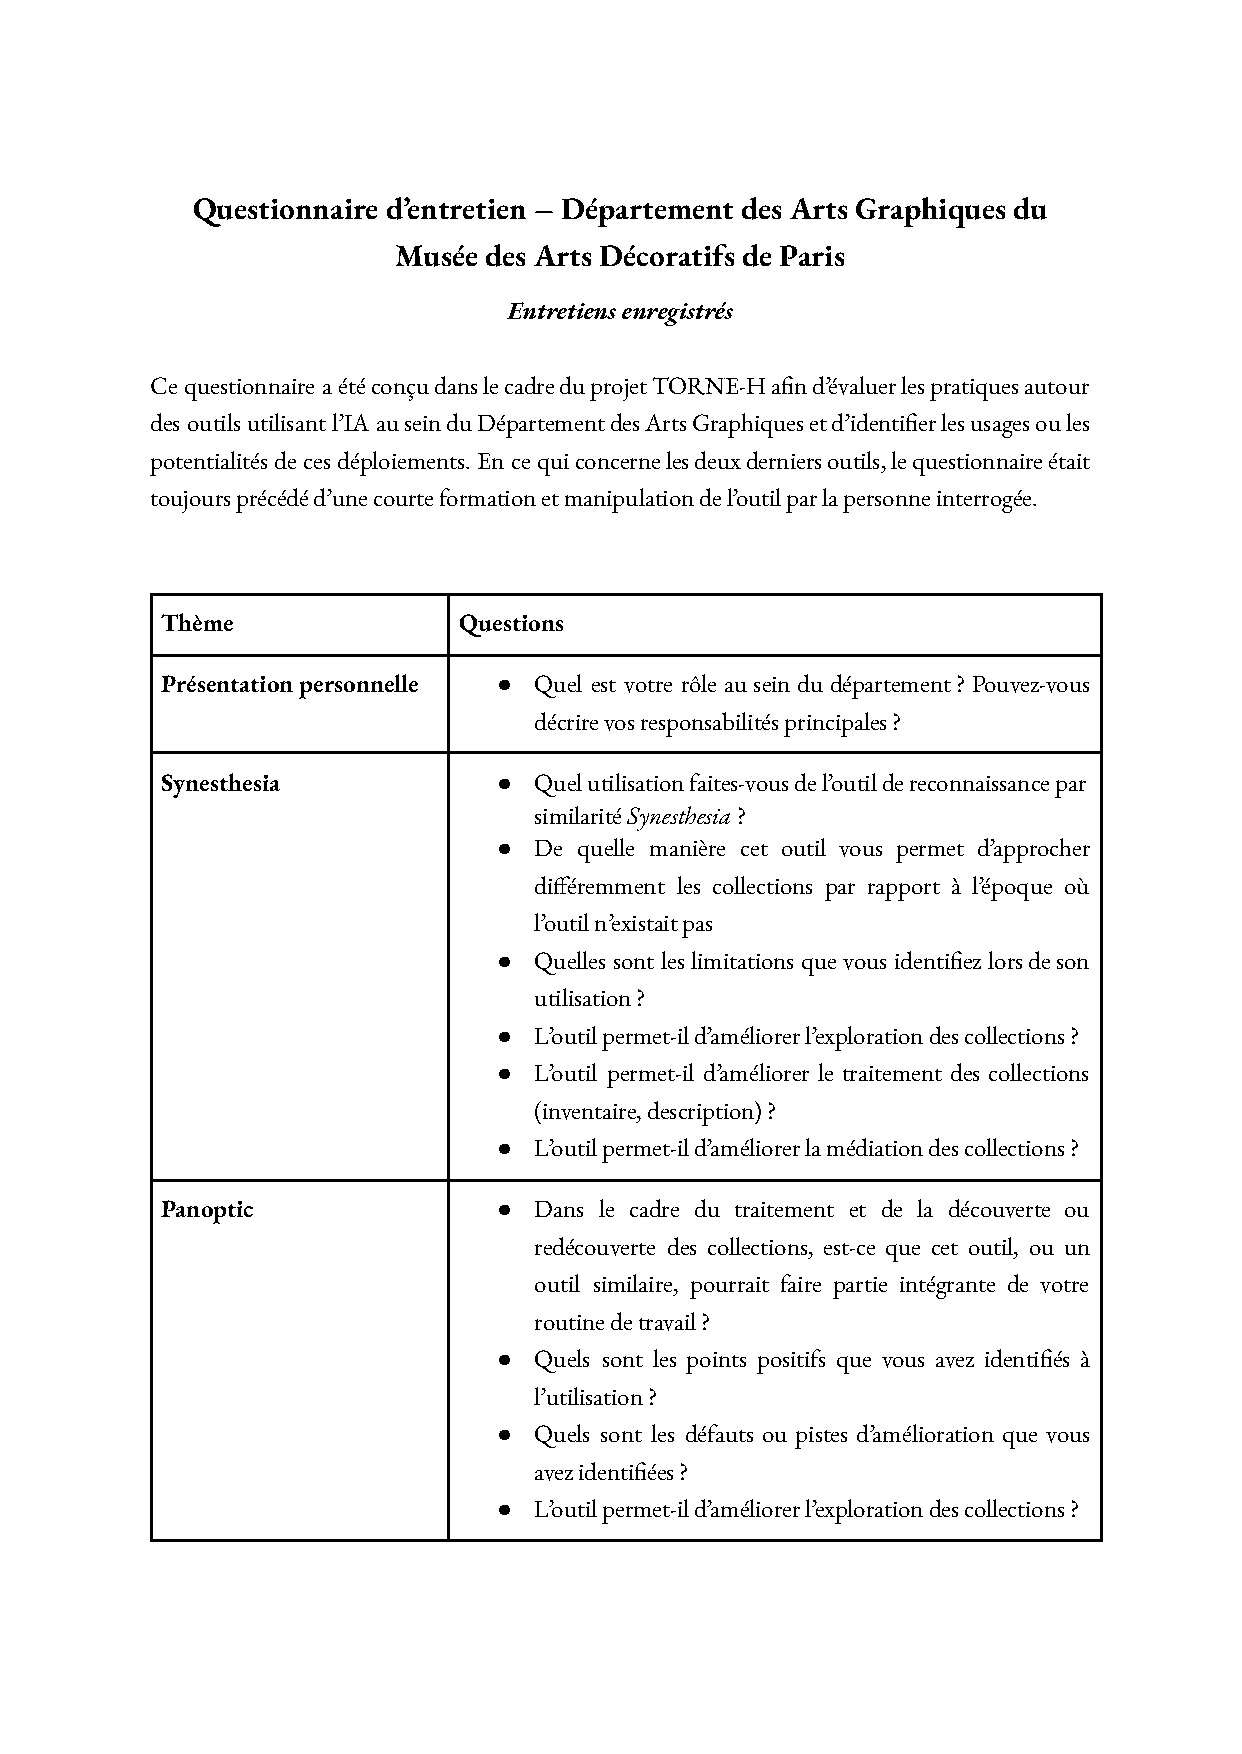
\includepdf[pages=-, pagecommand={}, scale=0.98]{Annexes/Questionnaire_d_entretien_IA_2025.pdf}

\chapter[Utilisation de Copilot]{Utilisation de Github Copilot - Modèle Claude Sonnet 3.5 pour script de scrapping}
\label{sec:Copilot}

Baghate: explique moi ligne par ligne ce que fait cette fonction

\begin{minted}[fontsize=\small,breaklines]{python}

def download\_gallica\_image(url, index):

try:

parts = url.split('ark:')

if len(parts) > 1:

image\_url = f"https://gallica.bnf.fr/iiif/ark:{parts[1]}/f1/full/max/0/default.jpg"

output\_path = os.path.join(output\_dir, f"image\_{index:02d}.jpg")

return download\_image(image\_url, output\_path)

except Exception as e:

print(f"Erreur lors du téléchargement depuis Gallica : {e}")

return False

return False

\end{minted}

GitHub Copilot: Voici une explication ligne par ligne de la fonction :

\begin{minted}[fontsize=\small,breaklines]{python}

def download\_gallica\_image(url, index):

  Déclaration de la fonction qui prend en paramètres une URL et un index pour nommer le fichier.

try:


  On tente d'exécuter le bloc de code suivant, afin de gérer proprement les erreurs.

parts = url.split('ark:')

  On découpe la chaîne de caractères 'url' à chaque occurrence de "ark:".

  Cela permet d'extraire la partie de l'URL qui suit "ark:".

if len(parts) > 1:

  On vérifie que le découpage a bien renvoyé plus d'une partie,

  ce qui signifie que "ark:" était présent dans l'URL.

image\_url = f"https://gallica.bnf.fr/iiif/ark:{parts[1]}/f1/full/max/0/default.jpg"

  On reconstruit l'URL de l'image en insérant la partie extraite (parts[1]) dans un format IIIF standard.

  Cette URL vise à obtenir l'image en haute résolution depuis Gallica.

output\_path = os.path.join(output\_dir, f"image\_{index:02d}.jpg")

  On génère le chemin complet où l'image sera enregistrée.

  'output\_dir' est le répertoire de sortie et 'index:02d' formate l'index sur 2 chiffres (par ex. 01, 02).

return download\_image(image\_url, output\_path)

  On lance le téléchargement de l'image en appelant la fonction 'download\_image'

  avec l'URL de l'image et le chemin de sortie, puis on retourne le résultat de cette opération.

except Exception as e:

  Si une erreur (Exception) survient dans le bloc try...

print(f"Erreur lors du téléchargement depuis Gallica : {e}")

  ... on affiche un message d'erreur incluant les détails de l'exception.

return False

  On retourne False pour indiquer que le téléchargement a échoué.

return False

  Si aucune condition n'a été satisfaite (par exemple, si "ark:" n'est pas trouvé dans l'URL),

  on retourne False par défaut.

\end{minted}

Cette fonction permet ainsi de transformer une URL de Gallica en URL IIIF correspondant à l'image, puis de la télécharger et de l'enregistrer localement.

Baghate: explique moi cette ligne

with open(output\_path, 'wb') as file:

GitHub Copilot: Cette ligne utilise le gestionnaire de contexte pour ouvrir un fichier en mode écriture binaire. Voici le détail :

\begin{minted}[fontsize=\small,breaklines]{python}

with open(output\_path, 'wb') as file:

\end{minted}

- **open(output\_path, 'wb')** : Ouvre le fichier situé à l'emplacement spécifié par la variable output\_path en mode "écriture binaire" ('wb'). Le mode binaire est utilisé pour écrire des données sous forme de bytes (comme des fichiers images).

- **as file** : Associe le fichier ouvert à la variable locale file, qui sera utilisée dans le bloc d'instructions suivant pour écrire dans le fichier.

- **with** : Le mot-clé with permet d'utiliser le gestionnaire de contexte. Cela garantit que lorsque le bloc est terminé, le fichier est automatiquement fermé, même en cas d'erreur, sans avoir à fermer explicitement le fichier avec file.close().

Baghate: explique moi cette ligne

\begin{minted}[fontsize=\small,breaklines]{python}

for chunk in response.iter\_content(1024):

\end{minted}

GitHub Copilot: Cette ligne itère sur le contenu de la réponse HTTP en découpant les données en blocs de 1024 octets. Cela permet d'écrire progressivement (en streaming) le contenu dans un fichier sans charger tout le fichier en mémoire.

Baghate: je veux définir une fonction pour scrapper des images, j'ai les url de ces images dans un csv, dans une colonne "URL" c'est le csv dans le variable input\_csv, et certaines images sont sur Gallica et d'autres sur le site des bibliothèques spécialisées de Paris mais je ne veux pas que tu me donnes juste le code sans rien, explique moi plutôt comment je dois m'y prendre ,quelles sont les étapes et ne me donne pas le réponse sauf si je te la demande

GitHub Copilot: Je vais vous guider à travers les étapes nécessaires pour construire cette fonction :

1. **Lecture du CSV**

- Il faut d'abord lire le fichier CSV avec pandas

- Vérifier que la colonne "URL" existe bien

- S'assurer que le CSV est bien encodé

2. **Identification de la source**

- Pour chaque URL, il faut déterminer si elle provient de :

* Gallica (contient "gallica.bnf.fr")

* Bibliothèques spécialisées de Paris (contient "bibliotheques-specialisees.paris.fr")

- Prévoir un cas par défaut si l'URL ne correspond à aucune source connue

3. **Traitement spécifique par source**

- Pour Gallica :

* Transformer l'URL en format IIIF

* Gérer le téléchargement direct

- Pour les Bibliothèques de Paris :

* Utiliser Selenium pour naviguer sur la page

* Extraire l'URL de l'image

* Gérer le téléchargement

4. **Gestion des erreurs et logging**

- Prévoir un système pour :

* Noter les échecs de téléchargement

* Enregistrer les numéros de lignes problématiques

* Gérer les timeouts et autres erreurs

5. **Sauvegarde des images**

- Créer le dossier de sortie s'il n'existe pas

- Nommer les fichiers de manière cohérente

- Vérifier l'intégrité des images téléchargées

Voulez-vous que nous commencions par implémenter une de ces étapes en particulier ?

Baghate: aide moi, propose moi juste l'étape d'après, là j'ai voulu vérifier que l'url commence par Gallica, après du coup on télécharge l'image en modifiant l'url qui se trouve dans le csv dans la colonne "URL" en y ajoutant "/f1/full/max/0/default.jpg"

GitHub Copilot: Je vois que vous avez commencé la vérification pour Gallica, mais il y a une erreur dans votre condition. Voici comment corriger et poursuivre :

1. D'abord, il faut lire le CSV et accéder aux URLs :

\begin{minted}[fontsize=\small,breaklines]{python}

def download\_image(input\_csv, output\_folder):

  Lire le CSV

df = pd.read\_csv(input\_csv)

  Pour chaque ligne du CSV

for index, row in df.iterrows():

url = row['URL']    Récupérer l'URL de la colonne

  Vérifier si c'est une URL Gallica

if url.startswith("https://gallica"):

  Ici nous traiterons la transformation de l'URL

\end{minted}

Voulez-vous que je continue avec la partie transformation de l'URL Gallica ?

Baghate: pourquoi on dit "for index" ? je ne comprends pas ?

GitHub Copilot: Le `index` dans `for index, row in df.iterrows():` représente la position de chaque ligne dans le DataFrame. C'est important pour plusieurs raisons :

1. **Nommage des fichiers** : L'index permet de donner un nom unique à chaque image téléchargée

\begin{minted}[fontsize=\small,breaklines]{python}

output\_path = f"image\_{index}.jpg"    Exemple: image\_0.jpg, image\_1.jpg, etc.

2. **Traçabilité** : Si une erreur survient, on peut facilement identifier quelle ligne du CSV pose problème

print(f"Erreur à la ligne {index} du CSV")

\end{minted}

3. **Correspondance** : L'index permet de faire le lien entre :

- L'image téléchargée

- La ligne dans le CSV original

- Les métadonnées associées

C'est comme une étiquette numérotée qui nous aide à suivre chaque image dans le processus de téléchargement.

Baghate: j'ai essayé de faire la partie conversion en IIIF des urls gallica, qu'est-ce que tu en penses ?

GitHub Copilot: Il y a quelques points à améliorer dans votre code actuel :

1. **Problème de récursion** : Vous appelez `download\_image()` à l'intérieur de `download\_image()`, ce qui créera une boucle infinie. Il faudrait plutôt avoir deux fonctions distinctes :

- Une pour le téléchargement général

- Une pour le téléchargement spécifique à Gallica

2. **Variable non définie** : Vous utilisez `folder` au lieu de `output\_folder`

3. **Problème de return** : Le `return` dans la boucle va arrêter la fonction après la première image

Voici une suggestion de correction :

\begin{minted}[fontsize=\small,breaklines]{python}

def download\_gallica\_image(url, output\_path):

  Fonction spécifique pour télécharger une image de Gallica

try:

response = requests.get(url, stream=True)

if response.status\_code == 200:

with open(output\_path, 'wb') as file:

\begin{minted}[fontsize=\small,breaklines]{python}

for chunk in response.iter\_content(1024):

file.write(chunk)

return True

except Exception as e:

print(f"Erreur: {e}")

return False


def download\_images(input\_csv, output\_folder):

df = pd.read\_csv(input\_csv)

for index, row in df.iterrows():

url = row['URL']


if url.startswith("https://gallica"):

parts = url.split('ark:')

image\_url = f"https://gallica.bnf.fr/iiif/ark:{parts[1]}/f1/full/max/0/default.jpg"

output\_path = os.path.join(output\_folder, f"image\_{index:02d}.jpg")

success = download\_gallica\_image(image\_url, output\_path)


if success:

print(f"Image {index} téléchargée avec succès")

\end{minted}

Cette version sépare les responsabilités et évite les problèmes de récursion. Voulez-vous que je vous explique plus en détail certaines parties ?

Baghate: en gros j'ai l'impression que ce qu'on pourrait faire c'est faire une fonction download\_image, et faire deux autrs fonctions dépendant de si c'est sur gallica ou le site des bibliothèques, est-ce que ça semblerait pertinent une première fonction qui appellerait les deux autres ? En termes logique vaudrait-il mieux pas du coup d'abord définir une fonction gallica et une fonction bib et enfin seulement faire une fonction download\_image qui activerait le téléchargement suivant l'un ou l'autre en fonction de l'adresse qui se trouve dans la colonne URL du csv ?

GitHub Copilot: Oui, votre raisonnement est très pertinent ! En termes de conception logicielle, il est en effet préférable de :

1. **Définir d'abord les fonctions spécialisées** :

- Une fonction pour Gallica qui sait gérer les spécificités IIIF

- Une fonction pour les Bibliothèques de Paris qui sait gérer Selenium

2. **Puis créer la fonction principale** qui :

- Lit le CSV

- Analyse l'URL

- Appelle la fonction appropriée

- Gère les erreurs globales

Cette approche suit le principe de "séparation des responsabilités" où chaque fonction a un rôle précis :

graph TD

A[download\_image] --> B{URL de quelle source?}

B -->|Gallica| C[download\_gallica]

B -->|Bibliothèques| D[download\_bib]

C --> E[Téléchargement]

D --> E[Téléchargement]

Je vous suggère de commencer par écrire les fonctions spécialisées avant la fonction principale. Voulez-vous qu'on commence par restructurer dans cet ordre ?

Baghate: donc dans l'ordre j'ai d'abord la fonction download\_image qui ne me sert qu'à distinguer la source des images c'est ça ? dans cette fonction je ne transforme pas encore l'URL gallica en format IIIF ?

GitHub Copilot: Exactement ! La fonction `download\_image` devrait servir uniquement à :

1. Lire le CSV

2. Identifier la source de chaque image

3. Appeler la fonction appropriée

Voici une suggestion de structure :

\begin{minted}[fontsize=\small,breaklines]{python}

def download\_image(input\_csv, output\_folder):

  Lire le CSV

df = pd.read\_csv(input\_csv)

  Pour chaque URL


for index, row in df.iterrows():

url = row['URL']

  Identifier la source et appeler la fonction appropriée

if "gallica.bnf.fr" in url:

download\_gallica(url, index, output\_folder)

elif "bibliotheques-specialisees.paris.fr" in url:

download\_bib(url, index, output\_folder)

else:

print(f"Source non reconnue pour l'URL à la ligne {index}")

\end{minted}

La transformation en format IIIF se fera dans la fonction `download\_gallica()`, car c'est une spécificité de Gallica. Chaque fonction spécialisée gère ses propres particularités.

Baghate: ah j'avais demandé de ne pas tout de suite me montrer le code, mais de ne me le montrer que si je demande, bon pour cette fois ça ira, mais fais attention.

Qu'est-ce que tu penses de ma fonction download\_image ?

GitHub Copilot: Désolé pour avoir donné le code directement. Analysons votre fonction `download\_image` :

**Points positifs** :

- La logique de séparation des sources est bonne

- L'utilisation de `startswith()` pour identifier la source est claire

- Le message d'erreur pour les URLs non reconnues est utile

**Points à améliorer** :

1. `df.read\_csv(input\_csv)` n'est pas correct car :

- `df` est déjà défini globalement

- La méthode `read\_csv()` appartient à pandas, pas au DataFrame

2. Structure :

- La fonction fait à la fois la lecture du CSV et le routage vers les fonctions spécialisées

- Il serait plus propre de séparer ces responsabilités

3. Gestion des erreurs :

- Pas de try/except pour gérer les erreurs potentielles

- Pas de vérification que le CSV contient bien une colonne 'URL'

Voulez-vous que nous corrigions ces points un par un ?

Baghate: montre moi juste comment séparer la lecture du csv du reste pour séparer les responsabilités

GitHub Copilot: Voici comment vous pourriez séparer la lecture du CSV de la logique de téléchargement :

\begin{minted}[fontsize=\small,breaklines]{python}

def read\_url\_csv(input\_csv):

\end{minted}

"""Lecture du CSV et vérification de la colonne URL"""

\begin{minted}[fontsize=\small,breaklines]{python}

try:

df = pd.read\_csv(input\_csv)

if 'URL' not in df.columns:

raise ValueError("Le CSV ne contient pas de colonne 'URL'")

return df

except Exception as e:

print(f"Erreur lors de la lecture du CSV: {e}")

return None

def download\_image(input\_csv, output\_folder):

"""Gestion du téléchargement selon la source"""

df = read\_url\_csv(input\_csv)    Séparation de la lecture

if df is None:

return

for index, row in df.iterrows():

url = row['URL']

  ...reste de votre code existant...

\end{minted}

Cette séparation permet de :

- Isoler la lecture du CSV dans une fonction dédiée

- Gérer les erreurs de lecture du CSV indépendamment

- Vérifier la présence de la colonne URL

- Rendre le code plus maintenable

Voulez-vous que j'explique plus en détail certains aspects ?

Baghate: df.read\_csv(input\_csv) n'est pas correct car :

df est déjà défini globalement

La méthode read\_csv() appartient à pandas, pas au DataFrame

explique moi plus ce point, je ne comprends pas, c'est pas comme ça qu'on lit un csv ?

GitHub Copilot: Non, il y a une confusion dans la syntaxe. Voici l'explication :

1. **Comment lire un CSV avec pandas** :

- La bonne syntaxe est : `pd.read\_csv()` car c'est une fonction de pandas

- On l'assigne généralement à une variable : `df = pd.read\_csv()`

2. **Ce qui ne va pas dans votre code** :

- Vous écrivez `df.read\_csv()` ce qui signifie que vous essayez d'appeler une méthode `read\_csv` sur un DataFrame existant

- De plus, `df` est déjà défini globalement dans votre code (ligne 3 de votre notebook)

3. **La correction** :

\begin{minted}[fontsize=\small,breaklines]{python}

def download\_image(input\_csv, output\_folder):

df = pd.read\_csv(input\_csv)    Correct

  ...reste du code...

\end{minted}

C'est comme si vous aviez une voiture (pandas) avec une fonction "démarrer". Vous ne dites pas à la voiture démarrée (df) de démarrer à nouveau, vous utilisez la fonction démarrer de la voiture (pandas).

Baghate: je préfère garder la lecture du csv là où elle est, et pour les try except si je comprends bien c'est par exemple si l'url ne renvoie pas 200 ou des choses comme ça ? Si je l'implémente comme ça c'est bon ?

GitHub Copilot: La structure de votre gestion d'erreurs n'est pas tout à fait optimale. Voici pourquoi :

1. **Problème avec l'ordre actuel** :

- Vous essayez d'abord de faire un `requests.get(image\_url)` avant même d'avoir lu le CSV et obtenu une URL

- La variable `image\_url` n'est pas définie à ce stade

- L'`index` n'est pas non plus défini quand vous l'utilisez dans le message d'erreur

2. **Suggestion d'organisation** :

\begin{minted}[fontsize=\small,breaklines]{python}

def download\_image(input\_csv, output\_folder):

try:

  1. D'abord lire le CSV

df = pd.read\_csv(input\_csv)

  2. Parcourir les URLs

for index, row in df.iterrows():

try:

\end{minted}

url = row['URL']

\begin{minted}[fontsize=\small,breaklines]{python}

if url.startswith("https://gallica"):

download\_gallica(url, index, output\_folder)

elif url.startswith('https://bibliotheques'):

download\_bib(url, index, output\_folder)

else:

print(f"Source non reconnue pour l'URL à la ligne {index}")

except Exception as e:

print(f"Erreur ligne {index}: {e}")

continue    Passer à l'URL suivante

except Exception as e:

print(f"Erreur lors de la lecture du CSV : {e}")

return False

\end{minted}

Cette structure permet de :

- Gérer les erreurs de lecture du CSV

- Gérer séparément les erreurs pour chaque URL

- Continuer le traitement même si une URL échoue

Voulez-vous que j'explique plus en détail certains aspects ?

Baghate: Si je reprends notre plan :

1.Lecture du CSV

Il faut d'abord lire le fichier CSV avec pandas

Vérifier que la colonne "URL" existe bien

S'assurer que le CSV est bien encodé

2.Identification de la source

Pour chaque URL, il faut déterminer si elle provient de :

Gallica (contient "gallica.bnf.fr")

Bibliothèques spécialisées de Paris (contient "bibliotheques-specialisees.paris.fr")

Prévoir un cas par défaut si l'URL ne correspond à aucune source connue

3.Traitement spécifique par source

Pour Gallica :

Transformer l'URL en format IIIF

Gérer le téléchargement direct

Pour les Bibliothèques de Paris :

Utiliser Selenium pour naviguer sur la page

Extraire l'URL de l'image

Gérer le téléchargement

4.Gestion des erreurs et logging

Prévoir un système pour :

Noter les échecs de téléchargement

Enregistrer les numéros de lignes problématiques

Gérer les timeouts et autres erreurs

5.Sauvegarde des images

Créer le dossier de sortie s'il n'existe pas

Nommer les fichiers de manière cohérente

Vérifier l'intégrité des images téléchargées

On a fait l'étape 1 et 2 maintennant il faut qu'on entame l'étape 3, le scrapping en fonction de la source

GitHub Copilot: Oui, passons à l'étape 3 ! Commençons par définir la fonction pour Gallica.

Pour Gallica, nous devons :

1. Prendre l'URL originale

2. La transformer en format IIIF (ajouter `/f1/full/max/0/default.jpg`)

3. Télécharger l'image

4. Sauvegarder avec un nom cohérent

Je propose qu'on commence par écrire la fonction `download\_gallica()`. Elle devra :

- Prendre en paramètres : l'URL, l'index (pour le nom du fichier) et le dossier de sortie

- Transformer l'URL

- Gérer les erreurs de téléchargement

- Retourner un booléen indiquant le succès ou l'échec

Voulez-vous qu'on écrive cette fonction étape par étape ?

Pour les Bibliothèques de Paris, ce sera plus complexe car il faudra :

1. Initialiser Selenium

2. Naviguer sur la page

3. Trouver l'élément contenant l'image

4. Extraire l'URL

5. Télécharger

Par quelle partie voulez-vous commencer ?

Baghate: est-ce que cette partie te semble bien ?

GitHub Copilot: Regardons la partie transformation d'URL que vous avez commencé :

\begin{minted}[fontsize=\small,breaklines]{python}

  1. Transformer l'URL

parts = url.split('ark:')

image\_url = f"https://gallica.bnf.fr/iiif/ark:{parts[1]}/f1/full/max/0/default.jpg"

\end{minted}

C'est un bon début, mais il faudrait :

1. **Vérifier que le split a fonctionné** :

- Vérifier que `parts` contient bien 2 éléments

- Gérer le cas où 'ark:' n'est pas dans l'URL

2. **Valider le format** :

- S'assurer que la partie après 'ark:' est bien formée

- Vérifier qu'il n'y a pas de caractères problématiques

3. **Gérer les erreurs explicitement** :

- Capturer l'exception avec un message clair

- Logger l'index de la ligne problématique

Voulez-vous qu'on améliore cette partie ?

Baghate: Comme ça c'est fonctionnel ? j'ai pas fait toutes les étapes que tu as recommandé parce que je pense que certaines sont dispensables

GitHub Copilot: Analysons votre code actuel :

\begin{minted}[fontsize=\small,breaklines]{python}

  1. Transformer l'URL

parts = url.split('ark:')

if len(parts) > 1:

image\_url = f"https://gallica.bnf.fr/iiif/ark:{parts[1]}/f1/full/max/0/default.jpg"

\end{minted}

C'est un bon début minimaliste qui couvre l'essentiel :

- ✅ Le split sur 'ark:'

- ✅ La vérification que le split a fonctionné avec `if len(parts) > 1`

- ✅ La construction de l'URL IIIF

Cependant, il manque :

- ❌ Le retour de l'URL transformée ou une valeur par défaut en cas d'échec

- ❌ La gestion des erreurs si `parts[1]` est malformé

Le minimum suggéré serait :

\begin{minted}[fontsize=\small,breaklines]{python}

def download\_gallica(url, index, output\_folder):

try:

  1. Transformer l'URL

parts = url.split('ark:')

if len(parts) > 1:

image\_url = f"https://gallica.bnf.fr/iiif/ark:{parts[1]}/f1/full/max/0/default.jpg"

  Continuer avec le téléchargement...

else:

print(f"URL invalide à la ligne {index}: pas d'identifiant ark")

return False

except Exception as e:

print(f"Erreur lors du traitement de l'URL ligne {index}: {e}")

return False

\end{minted}

Voulez-vous qu'on passe à l'étape du téléchargement maintenant ?

Baghate: comment ça il n'y pas le retour de l'url transformée ? elle n'est pas stockée dans la variable image\_url ?

C'est le "return False" que j'aurai dû mettre ? Mais ça veut dire quoi return False ?

GitHub Copilot: Vous soulevez deux points importants :

1. **Concernant l'URL transformée** :

- Oui, l'URL est bien stockée dans `image\_url`

- Mais cette variable n'est utilisée que dans le bloc `if`

- Si le `if` échoue, on ne sait pas ce qui se passe avec l'URL

2. **Concernant `return False`** :

- `return False` signifie que la fonction a échoué

- C'est une convention courante en Python :

- `True` = succès

- `False` = échec

- Cela permet au code appelant de savoir si l'opération a réussi

Exemple d'utilisation :

\begin{minted}[fontsize=\small,breaklines]{python}

\end{minted}

success = download\_gallica(url, index, output\_folder)

\begin{minted}[fontsize=\small,breaklines]{python}

if success:

print("Téléchargement réussi")

else:

print("Échec du téléchargement")

\end{minted}

Pour améliorer votre code :

\begin{minted}[fontsize=\small,breaklines]{python}

def download\_gallica(url, index, output\_folder):

try:

\end{minted}

  1. Transformer l'URL

parts = url.split('ark:')

\begin{minted}[fontsize=\small,breaklines]{python}

if len(parts) > 1:

image\_url = f"https://gallica.bnf.fr/iiif/ark:{parts[1]}/f1/full/max/0/default.jpg"

  Utiliser image\_url pour le téléchargement

return True    Si tout s'est bien passé

else:

print(f"URL invalide à la ligne {index}")

return False    Si l'URL n'est pas valide

except Exception as e:

print(f"Erreur: {e}")

return False    Si une erreur survient

\end{minted}

Baghate: pourquoi on dit "Exception as e", c'est quoi "e" on l'a pas définit ni rien

GitHub Copilot: Le `e` dans `except Exception as e` est une variable qui capture les détails de l'exception. C'est une convention en Python, mais on pourrait utiliser n'importe quel nom de variable.

Voici comment ça fonctionne :

1. Quand une erreur survient dans un bloc `try`, Python crée un objet Exception

2. Le `as e` capture cet objet dans la variable `e`

3. On peut ensuite utiliser `e` pour :

- Afficher le message d'erreur

- Examiner le type d'erreur

- Logger les détails

Exemple :

\begin{minted}[fontsize=\small,breaklines]{python}

try:

result = 1/0    Génère une erreur de division par zéro

except Exception as error:    On pourrait utiliser 'e', 'err', ou tout autre nom

print(f"Une erreur est survenue: {error}")    Affiche: "Une erreur est survenue: division by zero"

print(f"Type d'erreur: {type(error)}")    Affiche: "Type d'erreur: <class 'ZeroDivisionError'>"

\end{minted}

C'est utile pour :

- Le debugging

- La journalisation des erreurs

- Informer l'utilisateur de ce qui s'est mal passé

Baghate: parce que du coup dans "e" le code met le raison de l'erreur ? On a aps besoin de coder en dur les noms d'erreurs qu'il peut y avoir

GitHub Copilot: Exactement ! L'avantage d'utiliser `Exception as e` est que Python capture automatiquement tous les types d'erreurs possibles et leurs messages associés, sans qu'on ait besoin de les définir nous-mêmes.

Exemple :

\begin{minted}[fontsize=\small,breaklines]{python}

def download\_gallica(url, index, output\_folder):

try:

\end{minted}

parts = url.split('ark:')

\begin{minted}[fontsize=\small,breaklines]{python}

if len(parts) > 1:

image\_url = f"https://gallica.bnf.fr/iiif/ark:{parts[1]}/f1/full/max/0/default.jpg"

return True

except Exception as e:

  e contiendra automatiquement :

  - "Invalid URL" si l'URL est mal formée

  - "Connection timeout" si le serveur ne répond pas

  - "File not found" si le fichier n'existe pas

  etc...

print(f"Erreur ligne {index}: {e}")    e contient le message d'erreur approprié

return False

\end{minted}

C'est plus flexible que d'écrire tous les cas d'erreur possibles :

- On n'a pas besoin de prévoir toutes les erreurs

- Le message sera toujours pertinent

- C'est plus maintenable

- C'est plus court

Python gère les messages d'erreur de manière intelligente et les stocke dans la variable que nous nommons par convention `e`.

Baghate: pourquoi mon code est inatteignable ? et j'ai l'impression qu'il est redondant, si je lui dis déjà de print quelque chose si c'ets différent de status code 200 est-ce que je dois vraiment passer par un expect ?

GitHub Copilot: Votre code est inatteignable à cause de deux problèmes :

1. **Return prématuré** : Dans le premier bloc `try`, vous avez un `return True` après avoir créé l'`image\_url`. Ce `return` fait sortir de la fonction avant d'atteindre le code de téléchargement.

2. **Indentation incorrecte** : Les blocs "2. Télécharger" et "3. Sauvegarder" sont au même niveau que le premier `except`, ce qui les rend inaccessibles.

Concernant la redondance de la gestion d'erreurs, voici une version plus propre :

\begin{minted}[fontsize=\small,breaklines]{python}

def download\_gallica(url, index, output\_folder):

try:

\end{minted}

  1. Transformer l'URL

parts = url.split('ark:')

\begin{minted}[fontsize=\small,breaklines]{python}

if len(parts) <= 1:

\end{minted}

print(f"URL invalide à la ligne {index}")

return False

image\_url = f"https://gallica.bnf.fr/iiif/ark:{parts[1]}/f1/full/max/0/default.jpg"

  2. Télécharger

response = requests.get(image\_url, stream=True, timeout=10)

\begin{minted}[fontsize=\small,breaklines]{python}

if response.status\_code != 200:

\end{minted}

print(f'Problème url {index}: status code {response.status\_code}')

return False

  3. Sauvegarder

output\_path = os.path.join(output\_folder, f"image\_{index:02d}.jpg")

with open(output\_path, 'wb') as file:

\begin{minted}[fontsize=\small,breaklines]{python}

for chunk in response.iter\_content(1024):

file.write(chunk)

return True

except Exception as e:

print(f"Erreur pour l'URL Gallica ligne {index}: {e}")

return False

\end{minted}

Cette version :

- Utilise un seul bloc `try/except` global pour capturer les erreurs inattendues

- Vérifie le status code sans `try/except` redondant

- Garde une structure logique : transformation → téléchargement → sauvegarde

Baghate: pourquoi à la fin du  3 on met un return True ?

GitHub Copilot: Le `return True` à la fin du bloc  3 est important car il signale que toutes les étapes ont réussi avec succès :

1. Logique de la fonction :

- Si l'URL est invalide → `return False`

- Si le téléchargement échoue → `return False`

- Si tout fonctionne jusqu'à la fin → `return True`

2. Pourquoi c'est utile :

- Permet au code appelant de savoir si le téléchargement a réussi

- Aide à compter le nombre de téléchargements réussis

- Permet de gérer les erreurs au niveau supérieur

Exemple d'utilisation :

\begin{minted}[fontsize=\small,breaklines]{python}

\end{minted}

success = download\_gallica(url, index, output\_folder)

\begin{minted}[fontsize=\small,breaklines]{python}

if success:

successful\_downloads += 1

else:

failed\_downloads.append(index)

\end{minted}

Sans ce `return True`, la fonction retournerait `None` par défaut, ce qui ne permettrait pas de distinguer un succès d'une erreur non gérée.

Baghate: la méthode request.get permet de télécharger une image c'ets ça ? est-ce qu'il y a d'autres méthodes pour télécharger un contenu sur une page ou autre?

GitHub Copilot: Il existe plusieurs méthodes pour télécharger du contenu web en Python :

1. **requests.get()** (que vous utilisez) :

- Simple et efficace pour les requêtes HTTP basiques

- Bon pour télécharger des fichiers directement accessibles

\begin{minted}[fontsize=\small,breaklines]{python}

response = requests.get(url)

\end{minted}

2. **urllib** (bibliothèque standard Python) :

- Plus basique que requests

- Pas besoin d'installation externe

\begin{minted}[fontsize=\small,breaklines]{python}

import urllib.request

urllib.request.urlretrieve(url, "output.jpg")

\end{minted}

3. **wget** :

- Utile pour les téléchargements plus complexes

- Gère bien les interruptions/reprises

\begin{minted}[fontsize=\small,breaklines]{python}

import wget

wget.download(url, "output.jpg")

\end{minted}

4. **Selenium** (que vous utiliserez pour les Bibliothèques de Paris) :

- Pour les sites nécessitant une navigation

- Pour le contenu généré dynamiquement par JavaScript

\begin{minted}[fontsize=\small,breaklines]{python}

driver.get(url)

element = driver.find\_element(By.TAG\_NAME, "img")

image\_url = element.get\_attribute("src")

\end{minted}

5. **Beautiful Soup** :

- Pour extraire des données de pages HTML

- Souvent utilisé avec requests

\begin{minted}[fontsize=\small,breaklines]{python}

from bs4 import BeautifulSoup

soup = BeautifulSoup(response.content, 'html.parser')

images = soup.find\_all('img')

\end{minted}

Dans votre cas, `requests.get()` est le bon choix pour Gallica car :

- Les URLs IIIF sont directement accessibles

- Vous n'avez pas besoin de navigation complexe

- La méthode supporte le streaming (téléchargement par morceaux)

Baghate: est-ce qu'on ne pourrait pas tenter avec beautiful soup pour le site des bibliothèques ? Ah et est-ce possible de tester la fonction même si on a pas encore fait la partie download\_bib ?

GitHub Copilot: Pour les Bibliothèques de Paris, BeautifulSoup ne serait pas le meilleur choix car :

1. **Contenu dynamique** :

- Le site utilise JavaScript pour charger les images

- BeautifulSoup ne peut lire que le HTML statique

- Les URLs des images ne seraient pas accessibles

2. **Selenium est nécessaire** car :

- Il peut interagir avec la page web

- Il attend le chargement du JavaScript

- Il peut accéder au contenu dynamique

Pour tester la fonction `download\_gallica` sans avoir `download\_bib`, vous pouvez :

1. Créer un stub temporaire :

\begin{minted}[fontsize=\small,breaklines]{python}

def download\_bib(url, index, output\_folder):

"""Fonction temporaire pour les tests"""

print(f"Téléchargement bibliothèque non implémenté pour ligne {index}")

return False

\end{minted}

2. Tester avec un CSV ne contenant que des URLs Gallica :

\begin{minted}[fontsize=\small,breaklines]{python}

  Test avec quelques URLs

test\_df = pd.DataFrame({

'URL': [

'https://gallica.bnf.fr/ark:/12148/btv1b10234567/f1',

'https://gallica.bnf.fr/ark:/12148/btv1b89876543/f1'

]

})

test\_df.to\_csv('test\_gallica.csv', index=False)

\end{minted}

Vous pourrez ainsi tester la partie Gallica pendant que vous développez la partie bibliothèques.

Baghate: Bon super ça marche très bien, maintenant la partie difficile,  là j'ai repris la config de Selenium que j'avais trouvé ailleurs, est-ce que ça te semble bien ? Mais d'ailleurs j'ai un doute pour la ligne driver.get, comment je lui dis que c'est l'url qui se trouve dans le csv ? est-ce for url in df['URL'] doit venir avant ?

GitHub Copilot: Analysons votre code pour la partie Selenium.

**Configuration Selenium** :

- ✅ Les options de Chrome sont bien configurées

- ✅ Le mode headless est activé

- ✅ La gestion du répertoire temporaire est correcte

**Problèmes dans la structure actuelle** :

1. La boucle `for url in df['URL']` est mal placée car :

- Le driver est initialisé avant la boucle

- `df` n'est pas accessible dans cette fonction

- On ne devrait traiter qu'une seule URL à la fois

Voici comment restructurer la fonction :

\begin{minted}[fontsize=\small,breaklines]{python}

def download\_bib(url, index, output\_folder):

\end{minted}

"""Fonction pour interagir avec les pages des bibliothèques spécialisées de Paris

Args:

url (str): URL de la page à scraper

index (int): Index pour nommer l'image

output\_folder (str): Dossier de destination

"""

\begin{minted}[fontsize=\small,breaklines]{python}

try:

\end{minted}

  Configuration Selenium

chrome\_driver\_path = "/home/mathieu/snap/chromium/chromedriver-linux64/chromedriver"

service = Service(chrome\_driver\_path)

user\_data\_dir = tempfile.mkdtemp()

options = webdriver.ChromeOptions()

options.add\_argument("--no-sandbox")

options.add\_argument(f"--user-data-dir={user\_data\_dir}")

options.add\_argument("--headless")

options.add\_argument("--disable-dev-shm-usage")

options.add\_argument("--remote-debugging-port=9222")

options.add\_argument("--disable-gpu")

  Initialiser le navigateur

driver = webdriver.Chrome(service=service, options=options)

\begin{minted}[fontsize=\small,breaklines]{python}

try:

  Naviguer vers l'URL

driver.get(url)

time.sleep(5)    Attendre le chargement

  Chercher l'image (à compléter)

images = driver.find\_elements(By.TAG\_NAME, "img")

  ... logique de récupération d'image ...

return True

finally:

driver.quit()    Toujours fermer le navigateur

except Exception as e:

print(f"Erreur pour l'URL bibliothèque ligne {index}: {e}")

return False

\end{minted}

Les changements principaux :

- La fonction ne traite qu'une seule URL

- Le driver est fermé proprement avec `finally`

- La structure suit le même pattern que `download\_gallica`

Voulez-vous qu'on passe à l'implémentation de la recherche d'image ?

Baghate: la solution me semble bien mais avant de l'appliquer j'ai une question si la boucle for est mal placée, pourquoi elle n'est pas du tout reprise dans la version que tu propose ? Comment il fait pour trouver l'url là ?

GitHub Copilot: La boucle `for` n'est pas nécessaire dans la fonction `download\_bib()` car l'itération sur les URLs est déjà gérée dans la fonction principale `download\_image()`. Regardons le flux :

1. **Dans `download\_image()`** :

\begin{minted}[fontsize=\small,breaklines]{python}

for index, row in df.iterrows():

try:


url = row['URL']

if url.startswith("https://gallica"):

download\_gallica(url, index, output\_folder)

elif url.startswith('https://bibliotheques'):

download\_bib(url, index, output\_folder)    Chaque URL est passée ici

\end{minted}

2. **Dans `download\_bib()`** :

- La fonction reçoit une seule URL comme paramètre

- Elle n'a pas besoin d'itérer car elle traite une seule URL à la fois

- C'est comme `download\_gallica()` qui ne traite qu'une URL à la fois

La structure actuelle crée une double boucle inutile :

1. Une dans `download\_image()`

2. Une dans `download\_bib()`

C'est pourquoi j'ai suggéré de retirer la boucle de `download\_bib()` et de laisser la fonction principale `download\_image()` gérer l'itération sur toutes les URLs.

Voulez-vous que je montre comment modifier votre code actuel pour corriger ce problème ?

Baghate: j'ai tenté de reprendre ce que j'avais déjà fait à un autre moment, parce qu'il c'était avéré qu'il fallait d'abord dismiss les cookies avant de pouvoir procéder, je sais que c'est pas très bien implémenté, peux-tu m'expliquer en détaillant et me proposer les ajustements pour adapter ce petit bout de code à notre tâche. Déjà si j'ai bien compris c'est dans tous les cas au sein du premier "try" qu'on va faire tout le processus ? Après avoir chargé la page on va faire tous nos autres "try" qui vont être les étapes de navigation ?

GitHub Copilot: Analysons la structure actuelle et comment l'améliorer :

1. **Structure des blocs try/except**

- Le premier `try` est pour la configuration globale de Selenium

- Le deuxième `try` est pour les opérations de navigation

- C'est une bonne pratique d'avoir cette séparation

2. **Gestion des cookies** :

Votre code actuel :

\begin{minted}[fontsize=\small,breaklines]{python}

try:

body = WebDriverWait(driver, 5).until(

EC.presence\_of\_element\_located((By.TAG\_NAME, "body"))

)

ActionChains(driver).move\_to\_element(body).click().perform()

\end{minted}

Problèmes :

- `EC` n'est pas importé

- L'indentation est incorrecte

- La gestion des cookies devrait être une fonction séparée

Suggestion de restructuration :

\begin{minted}[fontsize=\small,breaklines]{python}


from selenium.webdriver.support.ui import WebDriverWait

from selenium.webdriver.support import expected\_conditions as EC

from selenium.webdriver.common.action\_chains import ActionChains


def download\_bib(url, index, output\_folder):

try:


  Configuration Selenium (votre code actuel est bon)

driver = webdriver.Chrome(service=service, options=options)

try:


  1. Charger la page

print(f"Chargement de la page {index}...")

driver.get(url)

time.sleep(5)

\end{minted}

\begin{minted}[fontsize=\small,breaklines]{python}

  2. Gérer les cookies

try:

dismiss\_cookies(driver)

except Exception as e:

print(f"Erreur cookies: {e}, on continue...")

  3. Chercher et télécharger l'image

  ... à implémenter ...

return True

finally:

driver.quit()

except Exception as e:

print(f"Erreur configuration Selenium ligne {index}: {e}")

return False

\end{minted}

\begin{minted}[fontsize=\small,breaklines]{python}

def dismiss\_cookies(driver):


"""Gère la fenêtre des cookies"""

wait = WebDriverWait(driver, 5)

body = wait.until(EC.presence\_of\_element\_located((By.TAG\_NAME, "body")))

ActionChains(driver).move\_to\_element(body).click().perform()

\end{minted}

Cette structure permet :

1. Une meilleure séparation des responsabilités

2. Une gestion plus claire des erreurs

3. Un code plus maintenable

Voulez-vous qu'on passe à l'implémentation de la recherche et du téléchargement de l'image ?

Baghate: ça me semble bien comme organisation, je vais l'appliquer, mais d'abord j'ai une question, est-ce que ça ne risque pas de nous amener à faire une fonction séparée pour chaque étape un peu compliquée ? Est-ce qu'il vaut mieux multiplier les fonctions qu'on appelle, ou est-ce qu'il vaut mieux avoir une logique compacte ?

GitHub Copilot: C'est une excellente question qui touche à des principes fondamentaux de conception logicielle.

**Avantages des fonctions séparées** :

- Code plus lisible et maintenable

- Plus facile à tester unitairement

- Réutilisable pour d'autres parties du code

- Plus facile à débugger

**Inconvénients** :

- Plus de complexité dans l'organisation du code

- Potentiellement plus difficile à suivre le flux d'exécution

- Surcharge possible si trop de petites fonctions

**Règle du pouce** :

1. Appliquer le principe de "responsabilité unique" :

- Une fonction devrait faire une seule chose

- Mais cette "chose" doit avoir un sens métier

2. Créer une fonction séparée si :

- Le code est réutilisable ailleurs

- La logique est complexe et mérite d'être isolée

- Le code fait plus de 20-30 lignes

Dans votre cas :

- `dismiss\_cookies()` mérite d'être séparé car :

- C'est une opération distincte

- Pourrait être réutilisée sur d'autres sites

- Isole la gestion des erreurs spécifiques aux cookies

Mais il ne faut pas tomber dans l'excès :


  Trop granulaire

\begin{minted}[fontsize=\small,breaklines]{python}

def click\_element(driver, element):

ActionChains(driver).move\_to\_element(element).click().perform()

[fontsize=\small,breaklines]{python}

def wait\_for\_body(driver):



return WebDriverWait(driver, 5).until(EC.presence\_of\_element\_located((By.TAG\_NAME, "body")))
\end{minted}
  Mieux

\begin{minted}[fontsize=\small,breaklines]{python}

def dismiss\_cookies(driver):

body = WebDriverWait(driver, 5).until(EC.presence\_of\_element\_located((By.TAG\_NAME, "body")))

ActionChains(driver).move\_to\_element(body).click().perform()

\end{minted}

Baghate: D'accord je vois, dans le cadre d'un fichier en .py on laisserait tout comme ça mais là vu que je suis dans un notebook est-ce que ça vaudrait le coût que je fasse une cellule par fonction par exemple ?

GitHub Copilot: Pour un notebook Jupyter, séparer les fonctions en cellules différentes présente plusieurs avantages :

1. **Lisibilité et Organisation** :

- Une cellule = une fonction logique

- Plus facile à modifier et tester individuellement

- Structure claire du workflow

2. **Debug et Tests** :

- Possibilité d'exécuter/tester chaque fonction séparément

- Voir les outputs intermédiaires

- Facilite le débogage


Structure suggérée pour votre notebook :


Cellule 1 : Imports et configuration générale

Cellule 2 : Fonction principale download\_image()

Cellule 3 : Fonction download\_gallica()

Cellule 4 : Fonction dismiss\_cookies()

Cellule 5 : Fonction download\_bib()

Cellule 6 : Variables et appel des fonctions

Cette organisation :

- Garde la logique modulaire

- Facilite les tests

- Permet de voir les résultats intermédiaires

- Reste cohérente avec les principes de clean code

Voulez-vous que je montre comment réorganiser votre code actuel en cellules ?

Baghate: ah oui tu placerais la fonction dismiss cookies avant celle download\_bib ?

GitHub Copilot: Oui, il est préférable de placer `dismiss\_cookies()` avant `download\_bib()` pour plusieurs raisons :

1. **Dépendances logiques** :

- `download\_bib()` utilise `dismiss\_cookies()`

- Il faut donc que `dismiss\_cookies()` soit définie avant

2. **Organisation du code** :

- Les fonctions "helper" (utilitaires) viennent généralement avant les fonctions principales

- Cela suit une hiérarchie du plus simple au plus complexe

Structure suggérée pour votre notebook :

Cellule 1: Imports et configuration

Cellule 2: download\_image()

  Fonction principale qui orchestre tout

Cellule 3: download\_gallica()

  Première fonction spécialisée

Cellule 4: dismiss\_cookies()

  Fonction utilitaire pour Selenium

Cellule 5: download\_bib()

  Deuxième fonction spécialisée qui utilise dismiss\_cookies

Cellule 6: Exécution

  Variables et appel des fonctions

Cette organisation permet de :

- Respecter les dépendances entre fonctions

- Avoir une progression logique dans le code

- Faciliter la lecture et la maintenance

Voulez-vous que je montre la structure détaillée de ces cellules ?

Baghate: Voilà j'ai repris l'organisation, est-ce que ça te semble bien jusque là ? Avant qu'on continue le code.

Ah et j'ai une question concernant la partie "Configuration Selenium" est-ce que je la laisse là où elle est, ou bien logiquement la fonction dismiss\_cookies() en a besoin et du coup ça coince ?

GitHub Copilot: La configuration de Selenium devrait rester dans `download\_bib()` pour plusieurs raisons :

1. **Gestion des ressources** :

- Le driver Selenium doit être initialisé une seule fois par session

- Il doit être fermé proprement après utilisation

- La fonction `download\_bib()` gère ce cycle de vie

2. **Injection de dépendance** :

- `dismiss\_cookies()` reçoit le driver comme paramètre

- Elle n'a pas besoin de connaître comment il est configuré

- Cela respecte le principe de séparation des responsabilités

Structure actuelle :

\begin{minted}[fontsize=\small,breaklines]{python}

def download\_bib(url, index, output\_folder):

try:

\end{minted}

  Configuration Selenium

chrome\_driver\_path = "/home/mathieu/snap/chromium/chromedriver-linux64/chromedriver"

service = Service(chrome\_driver\_path)

user\_data\_dir = tempfile.mkdtemp()

options = webdriver.ChromeOptions()

  ...configuration...

driver = webdriver.Chrome(service=service, options=options)

\begin{minted}[fontsize=\small,breaklines]{python}

try:

driver.get(url)

dismiss\_cookies(driver)    On passe le driver configuré

  ...reste du code...

finally:

driver.quit()

except Exception as e:

print(f"Erreur: {e}")

return False

\end{minted}

Cette organisation :

- ✅ Garde la configuration où elle est nécessaire

- ✅ Permet à `dismiss\_cookies()` d'être une fonction pure

- ✅ Facilite les tests et la maintenance

Voulez-vous qu'on passe à l'implémentation de la recherche d'image maintenant ?

Baghate: Donc l'étape d'après c'est de cliquer sur l'image pour qu'elle s'affiche dans une nouvelle fenêtre. J'ai copié le Xpath de l'image : /html/body/div[1]/div/div[1]/div/div[1]/div/div/div[2]/div/div[1]/div/div/div/main/div/div/div/div/div/div[1]/div/div/div[1]/img

Est-ce que la manière dont je l'ai fait te semble bien là au point   3

GitHub Copilot: Votre approche pour cliquer sur l'image utilise un XPath absolu, ce qui est fragile car :

1. **Les XPath absolus sont sensibles aux changements** :

- Si la structure HTML change légèrement

- Si le site est mis à jour

- Si l'élément est dynamiquement généré

2. **Suggestions d'amélioration** :

- Utiliser un sélecteur plus robuste (CSS ou XPath relatif)

- Ajouter une vérification que l'élément est bien une image

- Gérer le cas où l'image n'est pas trouvée

Voici une version plus robuste :

\begin{minted}[fontsize=\small,breaklines]{python}

\end{minted}

  3. Chercher et cliquer sur l'image

\begin{minted}[fontsize=\small,breaklines]{python}

try:

\end{minted}

  D'abord chercher par un sélecteur plus simple

image = WebDriverWait(driver, 10).until(

EC.presence\_of\_element\_located((By.CSS\_SELECTOR, "img.viewer-image"))

  ou By.XPATH, "//img[contains(@class, 'viewer-image')]"

)

  Vérifier que c'est bien une image

\begin{minted}[fontsize=\small,breaklines]{python}

if image.tag\_name == 'img':

image.click()

print(f"Image trouvée et cliquée ligne {index}")

else:

print(f"Élément trouvé mais ce n'est pas une image ligne {index}")

return False

except Exception as e:

print(f"Impossible de trouver l'image ligne {index}: {e}")

return False

\end{minted}

Avant d'implémenter ces changements, pourriez-vous :

1. Vérifier la classe CSS de l'image sur le site

2. Inspecter si d'autres attributs pourraient identifier l'image de manière unique

Baghate: je crois que c'est une classe CSS "event", c'est possible ?

GitHub Copilot: Si l'image a la classe CSS "event", nous pouvons modifier le sélecteur pour être plus spécifique :

\begin{minted}[fontsize=\small,breaklines]{python}

\end{minted}

  Dans download\_bib()

  3. Chercher et cliquer sur l'image

\begin{minted}[fontsize=\small,breaklines]{python}

try:

\end{minted}

  Attendre et trouver l'image avec la classe 'event'

image = WebDriverWait(driver, 10).until(

EC.presence\_of\_element\_located((By.CSS\_SELECTOR, "img.event"))

)

\begin{minted}[fontsize=\small,breaklines]{python}

if image.tag\_name == 'img':

\end{minted}

  Vérifier qu'on a bien trouvé une image

src = image.get\_attribute('src')

\begin{minted}[fontsize=\small,breaklines]{python}

if src:

image.click()

print(f"Image trouvée et cliquée ligne {index}")

else:

print(f"Image sans source trouvée ligne {index}")

return False

else:

print(f"Élément trouvé mais ce n'est pas une image ligne {index}")

return False

except Exception as e:

print(f"Impossible de trouver l'image ligne {index}: {e}")

return False

\end{minted}

Cette version :

- Utilise un sélecteur CSS plus simple et robuste

- Vérifie que l'élément est bien une image

- Vérifie que l'image a un attribut src

- Gère les différents cas d'erreur possibles

Pouvez-vous vérifier dans l'inspecteur du navigateur si l'image a d'autres classes ou attributs qui pourraient aider à l'identifier de manière unique ?

Baghate: la quatrième étape c'est de basculer sur la fenêtre qui vient de pop-up, comment faire ?

GitHub Copilot: Pour basculer sur la nouvelle fenêtre qui s'ouvre après avoir cliqué sur l'image, nous devons gérer les "handles" (identificateurs) de fenêtres dans Selenium. Voici comment ajouter cette étape :

\begin{minted}[fontsize=\small,breaklines]{python}

\end{minted}

  4. Basculer sur la nouvelle fenêtre

\begin{minted}[fontsize=\small,breaklines]{python}

try:

\end{minted}

  Attendre que la nouvelle fenêtre soit ouverte

WebDriverWait(driver, 10).until(lambda d: len(d.window\_handles) > 1)

  Basculer sur la nouvelle fenêtre

original\_window = driver.current\_window\_handle

\begin{minted}[fontsize=\small,breaklines]{python}

for window\_handle in driver.window\_handles:

if window\_handle != original\_window:

driver.switch\_to.window(window\_handle)

break

print(f"Basculé sur la nouvelle fenêtre pour l'image {index}")

except Exception as e:

print(f"Impossible de basculer sur la nouvelle fenêtre ligne {index}: {e}")

return False

\end{minted}

Ce code :

1. Attend l'ouverture de la nouvelle fenêtre

2. Garde une référence à la fenêtre originale

3. Bascule sur la nouvelle fenêtre

4. Gère les erreurs potentielles

Maintenant nous pourrons récupérer l'URL de l'image dans sa version haute résolution depuis cette nouvelle fenêtre.

Voulez-vous qu'on passe à l'étape de récupération de l'URL de l'image ?

Baghate: explique moi ce que c'est les handles s'il te plaît, mais aussi détaille moi la fonction lambda que t'as utilisé

GitHub Copilot: Les handles et la fonction lambda sont deux concepts importants dans ce contexte :

**Window Handles** :

- Ce sont des identifiants uniques pour chaque fenêtre/onglet du navigateur

- Stockés dans `driver.window\_handles` comme une liste

- Permettent de naviguer entre les fenêtres avec `driver.switch\_to.window(handle)`

Exemple :

\begin{minted}[fontsize=\small,breaklines]{python}


driver.window\_handles    ['CDwindow-123ABC', 'CDwindow-456DEF']

\end{minted}

**Fonction Lambda** :

\begin{minted}[fontsize=\small,breaklines]{python}


WebDriverWait(driver, 10).until(lambda d: len(d.window\_handles) > 1)

\end{minted}

Décortiquons :

- `lambda d:` : définit une fonction anonyme qui prend un paramètre `d` (le driver)

- `len(d.window\_handles) > 1` : condition à vérifier

- La fonction retourne `True` quand il y a plus d'une fenêtre

- `until()` attend que cette condition soit vraie

Version plus explicite équivalente :

\begin{minted}[fontsize=\small,breaklines]{python}

def wait\_for\_new\_window(driver):


return len(driver.window\_handles) > 1

WebDriverWait(driver, 10).until(wait\_for\_new\_window)

\end{minted}

L'avantage de la lambda :

- Plus concise

- Parfaite pour une condition simple utilisée une seule fois

- Couramment utilisée avec les fonctions `wait.until()`

Baghate: le return False à la fin de l'étape 3 empêche l'étape 4 de s'exécuter si j'ai bien compris, comment on peut faire pour maintenir la gestion d'erreur sans avoir ce problème ?

GitHub Copilot: You're correct - the `return False` in step 3 prevents step 4 from executing. Here's how to restructure the code to maintain error handling while allowing the flow to continue:

\begin{minted}[fontsize=\small,breaklines]{python}

def download\_bib(url, index, output\_folder):

\end{minted}

"""Function to interact with Paris specialized libraries pages"""

\begin{minted}[fontsize=\small,breaklines]{python}

try:

\end{minted}

  Configuration Selenium

  ...existing selenium setup code...

\begin{minted}[fontsize=\small,breaklines]{python}

try:

\end{minted}

  1. Load page

print(f"Loading page {index}...")

driver.get(url)

time.sleep(5)

  2. Handle cookies

\begin{minted}[fontsize=\small,breaklines]{python}

try:

\end{minted}

dismiss\_cookies(driver)

except Exception as e:

print(f"Cookie error: {e}, continuing...")

  3. Display image in new window

\begin{minted}[fontsize=\small,breaklines]{python}

try:

\end{minted}

image = WebDriverWait(driver, 10).until(

EC.element\_to\_be\_clickable((By.XPATH, "/html/body/div[1]/div/div[1]/div/div[1]/div/div/div[2]/div/div[1]/div/div/div/main/div/div/div/div/div/div[1]/div/div/div[1]/img"))

)

\begin{minted}[fontsize=\small,breaklines]{python}

if image.tag\_name == "img":

\end{minted}

image.click()

print(f"Image found and clicked line {index}")

else:

print(f"Element found but not an image line {index}")

raise Exception("Not an image element")

except Exception as e:

print(f"Cannot find image line {index}: {e}")

raise    Re-raise to be caught by outer try

  4. Switch to new window

\begin{minted}[fontsize=\small,breaklines]{python}

try:

\end{minted}

WebDriverWait(driver, 10).until(lambda d: len(d.window\_handles) > 1)

original\_window = driver.current\_window\_handle

\begin{minted}[fontsize=\small,breaklines]{python}

for window\_handle in driver.window\_handles:

if window\_handle != original\_window:

driver.switch\_to.window(window\_handle)

break

print(f"Switched to new window for image {index}")

except Exception as e:

print(f"Cannot switch to new window line {index}: {e}")

raise

return True

finally:

driver.quit()

except Exception as e:

print(f"Error in Selenium processing line {index}: {e}")

return False

\end{minted}

Key changes:

- Removed individual `return False` statements

- Used `raise` to propagate errors to the outer try/catch

- Maintained error logging at each step

- Single point of failure handling in the outer try/catch

- Added `return True` only after all steps succeed

This way:

1. Each step can fail and log its specific error

2. The error propagates up to the main try/catch

3. The driver always gets closed in the `finally` block

4. We only return `False` if any step fails completely

Baghate: je ne comprends pas bien ce que fait raise, et repasse en français si possible

GitHub Copilot: Je vais vous expliquer le `raise` en français :

Le mot-clé `raise` en Python permet de :

1. **Propager une erreur** vers le niveau supérieur

2. **Interrompre l'exécution** du bloc actuel

3. **Transmettre l'information** sur l'erreur

Exemple simplifié :

\begin{minted}[fontsize=\small,breaklines]{python}

def download\_bib(url, index, output\_folder):

try:

\end{minted}

  Niveau 1 : try principal

\begin{minted}[fontsize=\small,breaklines]{python}

try:

\end{minted}

  Niveau 2 : opérations sur l'image

image = WebDriverWait(driver, 10).until(...)

\begin{minted}[fontsize=\small,breaklines]{python}

if not image.tag\_name == "img":

raise Exception("Pas une image")    ← L'erreur est levée ici

  Ce code ne sera pas exécuté si l'erreur est levée

image.click()

except Exception as e:

print(f"Erreur image: {e}")

raise    ← L'erreur est propagée au niveau supérieur

except Exception as e:

print(f"Erreur globale: {e}")

return False    ← Gestion finale de l'erreur

\end{minted}

Sans `raise` :

- L'erreur serait "avalée" par le premier `except`

- Le code continuerait même en cas d'erreur

- On perdrait l'information sur l'erreur originale

Avec `raise` :

- L'erreur "remonte" jusqu'au `try/except` principal

- L'exécution s'arrête proprement

- On garde la trace complète de l'erreur

Voulez-vous un exemple plus concret avec votre code ?

Baghate: ok je pense avoir compris, et là est-ce que ma fonction download\_bib semble bien formée ?

GitHub Copilot: Analysons votre fonction `download\_bib` :

**Points positifs** :

- ✅ Bonne structure des blocs try/except imbriqués

- ✅ Configuration Selenium bien paramétrée

- ✅ Gestion des cookies séparée

- ✅ Messages d'erreur détaillés

**Points à améliorer** :

1. **Indentation** :

- Le bloc `  4. Basculer sur la nouvelle fenêtre` est mal indenté

- Il devrait être au même niveau que le bloc `  3.`

2. **Structure du try/except** :

- Le `finally` devrait être au même niveau que les blocs précédents

- Il y a un `raise` mais pas de gestion du téléchargement après

3. **Étapes manquantes** :

- Pas de code pour récupérer l'URL de l'image en haute résolution

- Pas de code pour télécharger l'image

- Pas de code pour sauvegarder l'image

Voici la structure suggérée :

\begin{minted}[fontsize=\small,breaklines]{python}

try:

\end{minted}

Configuration Selenium

\begin{minted}[fontsize=\small,breaklines]{python}

try:

1. Charger la page

2. Gérer cookies

3. Cliquer sur l'image

4. Basculer fenêtre

5. Récupérer URL haute résolution

6. Télécharger et sauvegarder

return True

finally:

driver.quit()

except Exception:

return False

\end{minted}

Voulez-vous qu'on ajoute les étapes manquantes ?

Baghate: Dis moi ce que tu pense du point n°5, j'ai repris la structure du point numéro 3 vu que c'est aussi une affaire de clic de bouton, mais juste je ne sais pas comment qualifier le "if dl.tag\_name =="

quelle catégorie mettre qui correspondrait ?

GitHub Copilot: Pour l'étape 5, la vérification du `tag\_name` n'est peut-être pas la plus appropriée car :

1. Le bouton de téléchargement est probablement :

- Un élément `<button>` ou

- Un élément `<a>` (lien) ou

- Un élément `<div>` avec un rôle de bouton

2. Une meilleure approche serait :

\begin{minted}[fontsize=\small,breaklines]{python}

\end{minted}

  5. Appuyer sur le bouton "Téléchargement"

\begin{minted}[fontsize=\small,breaklines]{python}

try:

\end{minted}

dl = WebDriverWait(driver, 10).until(

EC.element\_to\_be\_clickable((By.XPATH, "//*[@id='hires']"))

)

\begin{minted}[fontsize=\small,breaklines]{python}

if dl.get\_attribute('href') or dl.get\_attribute('role') == 'button':

dl.click()

print(f"Bouton téléchargement trouvé et cliqué ligne {index}")

else:

print(f"Élément trouvé mais ce n'est pas un bouton de téléchargement {index}")

raise Exception("Pas un bouton de téléchargement")

\end{minted}

Pour identifier le bon sélecteur, vous pourriez :

1. Inspecter l'élément dans le navigateur

2. Vérifier son type (`tag\_name`)

3. Regarder ses attributs (class, role, href, etc.)

Voulez-vous que je vous aide à identifier le bon sélecteur pour ce bouton ?

Baghate: dans le html c'est ça l'élément

GitHub Copilot: D'après le HTML que vous montrez, l'élément a :

1. **Attributs** :

- `id="hires"`

- `class="IR-ButtonContainer"`

2. **Type d'élément** :

- C'est un `<div>`, pas une `<img>`

Donc la vérification actuelle `if dl.tag\_name == "img"` n'est pas correcte. Il faudrait plutôt :

\begin{minted}[fontsize=\small,breaklines]{python}

\end{minted}

  5. Appuyer sur le bouton "Téléchargement"

\begin{minted}[fontsize=\small,breaklines]{python}

try:

\end{minted}

dl = WebDriverWait(driver, 10).until(

EC.element\_to\_be\_clickable((By.XPATH, "//*[@id='hires']"))

)

\begin{minted}[fontsize=\small,breaklines]{python}

if dl.tag\_name == "div":    Vérifie que c'est bien un div

dl.click()

print(f"Bouton téléchargement trouvé et cliqué ligne {index}")

else:

print(f"Élément trouvé mais ce n'est pas un div de téléchargement {index}")

raise Exception("Pas un bouton de téléchargement")

\end{minted}

On pourrait aussi utiliser un sélecteur plus précis comme  ou .

Baghate: Ok là c'est l'étape où il faut cocher une case, est que mon étape 6 semble adaptée pour ça ? ci-joint le screen du html pour savoir si le "if" est adapté

GitHub Copilot: D'après le HTML que vous montrez, votre étape 6 doit être ajustée car :

1. **Le sélecteur** est correct :

- `@id='checkConditions'` correspond bien à l'élément input

2. **La vérification du type** n'est pas correcte :

- Vous vérifiez `tag\_name == "div"`

- Mais c'est un `<input type="checkbox">`

Voici la correction suggérée :

\begin{minted}[fontsize=\small,breaklines]{python}

\end{minted}

  6. Cocher la checkbox

\begin{minted}[fontsize=\small,breaklines]{python}

try:

\end{minted}

checkbox = WebDriverWait(driver, 10).until(

EC.element\_to\_be\_clickable((By.XPATH, "//*[@id='checkConditions']"))

)

\begin{minted}[fontsize=\small,breaklines]{python}

if checkbox.get\_attribute('type') == "checkbox":

checkbox.click()

print(f"Checkbox des conditions trouvée et cochée ligne {index}")

else:

print(f"Élément trouvé mais ce n'est pas une checkbox ligne {index}")

raise Exception("Pas une checkbox")

except Exception as e:

print(f"Impossible de trouver la checkbox ligne {index}: {e}")

raise

\end{minted}

Les changements principaux :

- Vérification du type avec `get\_attribute('type')`

- Messages d'erreur plus précis

- Variable renommée en `checkbox` au lieu de `dl`

- Correction de la vérification de type

Baghate: Donc, on arrive vers le bout, avec le screenshot et mon étape 7 est-ce que tu peux me dire ce que t'en pense, notamment pour la condition if

GitHub Copilot: D'après le HTML montré, l'étape 7 doit être modifiée car :

1. **Le sélecteur est incorrect** :

- Vous utilisez `"//*[@id='checkConditions']"`

- Mais c'est un `<button type="button">`

2. **La condition if est incorrecte** :

- `if dl\_button.tag\_name == "?"` n'est pas valide

- Il faut vérifier que c'est un bouton

Voici la correction suggérée :

\begin{minted}[fontsize=\small,breaklines]{python}

\end{minted}

  7. Appuyer sur le bouton download

\begin{minted}[fontsize=\small,breaklines]{python}

try:

\end{minted}

dl\_button = WebDriverWait(driver, 10).until(

EC.element\_to\_be\_clickable((By.XPATH, "//button[contains(text(), 'Start the download')]"))

)

\begin{minted}[fontsize=\small,breaklines]{python}

if dl\_button.tag\_name == "button":

dl\_button.click()

print(f"Bouton de téléchargement final trouvé et cliqué ligne {index}")

else:

print(f"Élément trouvé mais ce n'est pas un bouton ligne {index}")

raise Exception("Pas un bouton de téléchargement")

except Exception as e:

print(f"Impossible de trouver le bouton de téléchargement final ligne {index}: {e}")

raise

\end{minted}

Les changements principaux :

- Sélecteur XPATH corrigé pour cibler le bon bouton

- Vérification du `tag\_name == "button"`

- Messages d'erreur plus précis

Baghate: maintenant la partie crawling sur les pages et tout est techniquement terminée, mais bien sur vu que rien n'est jamais simple il faut que le téléchargement soit un dossier zip contenant l'image. Donc pour moi il faut 1. dézipper le dossier, 2. extraire l'image du dossier dézipé, pour 3. la mettre dans le dossier /sortie tel que prévu par le code, et 4 en la renommant dans la continuité de notre nommage définit avant.

Est-ce qu'on laisse le crawling et téléchargement comme ça pour créer une nouvelle fonction ou bien on ajoute des étapes 8, 9, 10 etc..

GitHub Copilot: Je recommande de créer une nouvelle fonction séparée pour gérer le traitement du ZIP pour plusieurs raisons :

1. **Séparation des responsabilités** :

- `download\_bib()` s'occupe du crawling et du téléchargement

- Une nouvelle fonction gérerait l'extraction et le déplacement des fichiers

2. **Lisibilité et maintenance** :

- La fonction `download\_bib()` est déjà longue

- L'ajout d'étapes supplémentaires la rendrait trop complexe

Voici la structure suggérée :

\begin{minted}[fontsize=\small,breaklines]{python}

def process\_zip\_file(zip\_path, index, output\_folder):

\end{minted}

"""Traite le fichier ZIP téléchargé

Args:

zip\_path (str): Chemin du fichier ZIP téléchargé

index (int): Index pour le nommage

output\_folder (str): Dossier de destination final

Returns:

bool: True si succès, False si échec

"""

\begin{minted}[fontsize=\small,breaklines]{python}

try:

\end{minted}

  1. Dézipper dans un dossier temporaire

with tempfile.TemporaryDirectory() as temp\_dir:

with zipfile.ZipFile(zip\_path, 'r') as zip\_ref:

zip\_ref.extractall(temp\_dir)

  2. Trouver l'image dans le dossier extrait

\begin{minted}[fontsize=\small,breaklines]{python}

for root, \_, files in os.walk(temp\_dir):

for file in files:

if file.lower().endswith(('.jpg', '.jpeg', '.png')):


  3. Déplacer et renommer l'image

src = os.path.join(root, file)

dst = os.path.join(output\_folder, f"image\_{index:02d}{os.path.splitext(file)[1]}")

shutil.move(src, dst)

return True

return False

except Exception as e:

print(f"Erreur traitement ZIP ligne {index}: {e}")

return False

\end{minted}

Et modifier légèrement `download\_bib()` :

\begin{minted}[fontsize=\small,breaklines]{python}

\end{minted}

  Dans download\_bib(), après l'étape 7

  8. Attendre le téléchargement et traiter le ZIP

\begin{minted}[fontsize=\small,breaklines]{python}

try:

\end{minted}

time.sleep(5)    Attendre le téléchargement

downloads\_dir = os.path.expanduser("~/Downloads")

latest\_file = max([os.path.join(downloads\_dir, f) for f in os.listdir(downloads\_dir)],

key=os.path.getctime)

\begin{minted}[fontsize=\small,breaklines]{python}

if latest\_file.endswith('.zip'):

if not process\_zip\_file(latest\_file, index, output\_folder):
raise Exception("Échec du traitement du ZIP")

os.remove(latest\_file)    Nettoyer le ZIP

else:

raise Exception("Fichier téléchargé non trouvé")

except Exception as e:

print(f"Erreur traitement fichier téléchargé ligne {index}: {e}")

raise

\end{minted}

Cette approche :

- Maintient la clarté du code

- Facilite les tests et le débuggage

- Permet la réutilisation du traitement ZIP ailleurs si nécessaire

Qu'en pensez-vous ?

Baghate: ouai, j'ai quelques questions. D'abord la fonction process\_zip\_file doit être placée avant download\_bib c'ets ça ? comme pour la gestion des cookies ?

Ensuite, pourquoi pointer vers /Downloads ? C'est pour faire transiter d'abord le zip à cet endroit avant de l'ouvrir et de déplacer l'image ?

Est- ce que le code peut directement gérer le fait de supprimer les dossiers transitoires après extraction de l'image et son placement dans le bon dossier ?

Est-ce que shutil nécessite une installation ou un import particulier qu'on n'aurait pas encore ?

Dans la fonction process\_zip\_file je ne comprends pas le début de l'étape 2, à quoi correspont "for root, \_, files in ..." c'est quoi cet underscore ?

GitHub Copilot: Je vais répondre à vos questions dans l'ordre :

1. **Placement des fonctions** :

- Oui, `process\_zip\_file` devrait être définie avant `download\_bib` car elle est appelée par cette dernière

- Comme pour `dismiss\_cookies`, c'est une bonne pratique de définir les fonctions utilitaires avant

2. **Dossier Downloads** :

- C'est le comportement par défaut du navigateur

- Quand on clique sur "télécharger", Chrome sauvegarde automatiquement dans `~/Downloads`

- On ne peut pas directement intercepter le fichier avant qu'il n'arrive dans Downloads

3. **Gestion des fichiers temporaires** :

- Le code gère déjà le nettoyage grâce à :

\begin{minted}[fontsize=\small,breaklines]{python}

\end{minted}

with tempfile.TemporaryDirectory() as temp\_dir:

  Code d'extraction

  Une fois sorti du with, temp\_dir est automatiquement supprimé


- Le ZIP est supprimé explicitement avec : `os.remove(latest\_file)`

4. **Import shutil** :

- Oui, il faut ajouter l'import :

\begin{minted}[fontsize=\small,breaklines]{python}

\end{minted}
\begin{minted}[fontsize=\small,breaklines]{python}
import shutil    À ajouter avec les autres imports

\end{minted}

- C'est une bibliothèque standard Python, pas besoin de l'installer

5. **La boucle `for root, \_, files`** :

- C'est le résultat de `os.walk()` qui retourne 3 valeurs :

- `root` : le chemin du dossier courant

- `\_` : la liste des sous-dossiers (ignorée avec `\_`)

- `files` : la liste des fichiers

- L'underscore `\_` est une convention Python pour dire "on ignore cette valeur"

- On pourrait écrire `for root, dirs, files` mais comme on n'utilise pas `dirs`, on met `\_`

Je peux détailler davantage certains points si nécessaire.

\chapter[Formations Arkindex et Callico]{Formations préparées dans le cadre du Consortium PictorIA}
\label{sec:Formations}

\includepdf[pages=-, pagecommand={}, scale=0.98]{Annexes/Tutoriel_Utilisation_Arkindex.pdf}
\includepdf[pages=-, pagecommand={}, scale=0.98]{Annexes/Tutoriel_Callico.pdf}

%%%%%%%%%%%%%%%%%%

\backmatter % glossaire, index, table des figures, table des matières.. (la bibliographie a déjà été appelée)


\newpage{\pagestyle{empty}\cleardoublepage}

\cleardoublepage
\phantomsection
\listoffigures
\addcontentsline{toc}{chapter}{Liste des figures}


\cleardoublepage
\phantomsection
\listoftables
\addcontentsline{toc}{chapter}{Liste des tableaux}
%\printindex
%%%%%%%%%%%%%%%%%%%% Glossaire %%%%%%%%%%%%%%%%%%%%%%%%%%


%avec TexStudio: F9 pour compiler le glossaire (s'il y a aussi un index)

%mettre les entrées du glossaire ici ou les mettre dans un fichier à part que l'on appelle ici par 
%\loadglsentries{glossaire.tex}
\chapter*{Glossaire}
\label{sec:Glossaire}
\addcontentsline{toc}{chapter}{Glossaire}
\markboth{}{Glossaire}
\textbf{Annotation} = Cette tâche consiste à étiqueter et à organiser les données, en disant ce qu'il s'y trouve, de manière à ce qu’elles puissent être efficacement utilisées par les modèles de Machine Learning.

\textbf{Apprentissage auto supervisé} = \textit{Self-supervised learning}, est une position intermédiaire entre apprentissage non supervisé et supervisé. Le modèle apprend à partir de données non annotées mais structurées, en exploitant les relations intrinsèques entre les données. On l'utilise par exemple pour la supervision de parties manquantes d'une image ou pour générer les légendes d'images.

\textbf{Apprentissage machine} = \textit{Machine learning}, est une sous-catégorie de l'IA qui permet aux machines d'apprendre à partir de données sans être explicitement programmées pour chaque tâche, c'est basé sur des algorithmes qui optimisent leurs performances grâce à l'expérience.

\textbf{Apprentissage non supervisé} = \textit{Unsupervised learning}, ne comprends pas d'annotation de données, l’algorithme utilise un jeu de données brutes et obtient un résultat en se fondant sur la détection de similarités entre certaines de ces données. C'est l'approche du \textit{clustering} ou rapprochement par similarité, comme celui utilisé dans l'outil Panoptic.

\textbf{Apprentissage par renforcement} = \textit{Reinforcement learning}, processus dans lequel un programme extérieur évalue positivement ou négativement les résultats successifs de l’algorithme, l’accumulation des résultats permettant à l’algorithme d’améliorer ses performances jusqu’à ce qu’il atteigne un objectif préalablement fixé. L’apprentissage par renforcement est fréquemment utilisé dans la robotique. L’efficacité de l’apprentissage par renforcement a été attestée dans certains jeux stratégiques comme le jeu de go.

\textbf{Apprentissage profond} = \textit{Deep learning}, est une sous-catégorie de l'apprentissage machine qui utilise des réseaux de neurones artificiels profonds pour analyser des données complexes. Cette technique est capable de traiter des données volumineuses et non structurées (images, sons, vidéos), mais nécessite des ressources importantes en termes de puissances de calcul, ainsi qu'une grande quantité de données.

\textbf{Apprentissage supervisé} = \textit{Supervised learning}, repose sur l'utilisation de données annotées qui servent à former des algorithmes capables de classer des données ou de prédire des annotations. Ils nécessitent une intervention humaine. L’apprentissage supervisé recourt le plus souvent aux réseaux de neurones artificiels.

\textbf{Bash} = Interpréteur de commandes, sont équivalent Windows est le shell, il permet aux utilisateurs d'exécuter des instructions sur la ligne de commande, automatiser les tâches en utilisant des scripts et de gérer efficacement les fichiers, processus et ressources système.

\textbf{Boîte d'annotation} = \textit{Bounding box}, est un cadre rectangulaire tracé autour d'un objet ou d'une région d'intérêt dans une image numérique ou un espace 3D, afin d'en définir la position et la taille. Elle est couramment utilisée en vision par ordinateur, en traitement d'images et dans le développement de jeux vidéo pour des tâches telles que la détection d'objets, la détection de collisions ou l'annotation d'images. La boîte est généralement définie par les coordonnées de ses coins, par sa largeur et sa hauteur, ou par son centre et ses dimensions. Elle peut être alignée sur les axes (AABB) ou orientée (OBB) afin de mieux s'ajuster à la forme de l'objet. Bien qu'efficace et facile à calculer, une boîte englobante peut inclure des zones de fond et être moins précise que des méthodes plus détaillées comme la segmentation.

\textbf{Bruit} = Dans un processus automatisé, on parle de bruit quand les données contiennent des éléments indésirables, imprécis ou aléatoires qui ne reflètent pas fidèlement le signal ou l’information que l’on veut réellement analyser. Son opposé est le silence.

\textbf{CI/CD} = \textit{Continuous Integration/Continuous Delivery}, le CI/CD comble le fossé entre les activités et les équipes de développement et d'exploitation en imposant l'automatisation de la création, des tests et du déploiement des applications. Les pratiques DevOps usuelles peuvent impliquer le développement continu, le test continu, l'intégration continue, le déploiement continu et la surveillance continue des applications logicielles tout au long de leur cycle de vie.

\textbf{Clip} = \textit{Contrastive Language-Image Pre-training}, est un modèle de \textit{computer vision} développé par la société OpenAI (la société derrière ChatGPT), qui apprend à associer des images et leurs descriptions textuelles.


\textbf{CPU} = \textit{Central Processing Unit}, est constitué de milliards de transistors, le processeur (CPU) peut avoir plusieurs cœurs de traitement et est communément appelé le « cerveau » de l'ordinateur. Il est essentiel à tous les systèmes informatiques modernes, car il exécute les commandes et les processus nécessaires à votre ordinateur et à votre système d'exploitation.

\textbf{CSV} = \textit{Coma Separated Values}, est un fichier texte, par opposition aux formats dits « binaires ». Chaque ligne du texte correspond à une ligne du tableau et les virgules correspondent aux séparations entre les colonnes. Les portions de texte séparées par une virgule correspondent ainsi aux contenus des cellules du tableau.

\textbf{Centres de données} = \textit{Data centers}, sont des infrastructures composées d’un réseau d’ordinateurs et d’espaces de stockage. Ces infrastructures hautement sécurisées sont utilisées par les entreprises ou acteurs publics pour organiser, traiter, stocker et entreposer de grandes quantités de données.

\textbf{Data Scientist} = Généralement rattaché à la direction des systèmes d'information (DSI) d’une entreprise, le \textit{Data Scientist} a pour objectif d’analyser et d’exploiter toutes les datas des clients, des prospects ou bien encore des employés que l’entreprise récupère via différents canaux. L’objectif est de créer des modèles prédictifs et d’aider la prise de décision par la construction d'algorithmes.

\textbf{DevOps} = \textit{Development and operations}, est principalement par la promotion de l'automatisation et du suivi (monitoring) de toutes les étapes de la création d'un logiciel, depuis le développement, l'intégration, les tests, la livraison jusqu'au déploiement, l'exploitation et la maintenance des infrastructures.

\textbf{Docker} = Docker est une plateforme de conteneurisation open source qui permet de créer, déployer et gérer des applications virtualisées dans des conteneurs. Les conteneurs logiciels sont une forme de virtualisation légère qui offre une isolation pour les applications, rendant leur déploiement plus rapide et plus efficace par rapport aux machines virtuelles traditionnelles.

\textbf{Embeddings} = En apprentissage automatique, un \textit{embedding} désigne une technique d’apprentissage de représentations qui projette des données complexes et de haute dimension dans un espace vectoriel de dimension plus faible. Le terme désigne également la représentation obtenue, où des structures ou les relations significatives sont préservées. En tant que technique, il apprend ces vecteurs à partir de données telles que des mots, des images ou des interactions d’utilisateurs. Un espace vectoriel est un cadre mathématique dans lequel chaque entité est représentée par un vecteur, c’est-à-dire une suite ordonnée de valeurs numériques. Cette représentation permet d’exprimer des idées ou objets complexes sous la forme de points dans un espace à \textit{n} dimensions, rendant ainsi mesurables leurs similarités ou leurs différences.

\textbf{Espace vectoriel} = En \textit{machine learning}, la caractérisation d'une image par exemple sur base sur des embeddings. Ils sont des représentations vectorielles continues qui encapsulent le contexte et le sens des données. Ils traduisent des concepts complexes en un format numérique compact, capturant les relations sémantiques entre différentes entités. Cela se traduit par une représentation dense, de faible dimensionnalité, qui conserve des propriétés importantes des données d'origine.

\textbf{Fine-tuning} = Contrairement à l’entraînement initial (comme ce qui a été fait avec Clip par exemple) qui nécessite des jeux de données massifs, cet affinage se concentre sur des données plus restreintes et spécialisées. Il s’agit d’un processus itératif qui vise à améliorer la performance du modèle sur une tâche particulière, sans perdre les connaissances préalables acquises lors de l’entraînement initial.

\textbf{GPU} = \textit{Graphics Processing Unit}, c'est une unité de calcul assurant les fonctions de calcul d’image. Originellement les GPUs ont été développés pour les jeux vidéos et le calcul de déplacements en 2 ou 3 dimensions.

\textbf{Graphe de connaissance} = \textit{Knowledge graph}, est une base de connaissance modélisant ses données sous forme graphique. Beaucoup utilisé dans l'optimisation de moteurs de recherche, le plus connu est celui développé par Google qui fournit une information structurée et détaillée centrée sur l'objet de la recherche, en plus de la liste d'hyperliens vers d'autres sites. L'objectif est de permettre aux utilisateurs de résoudre leur requête sans avoir besoin de naviguer vers d'autres sites pour accéder aux informations capitales.

\textbf{HTR} = \textit{Handwritten Text Recognition}, c'est la reconnaissance automatique de caractères manuscrits sur une image.

\textbf{IDE} = \textit{Integrated development environment}, est une application logicielle qui aide les programmeurs à développer efficacement le code logiciel. Il augmente la productivité des développeurs en combinant les capacités telles que l'édition de logiciels, la construction, les tests et l'empaquetage dans une application facile à utiliser. De la même manière que les rédacteurs utilisent des éditeurs de texte et les comptables utilisent des feuilles de calcul, les développeurs de logiciels utilisent des IDE pour faciliter leur travail.

\textbf{IIIF} = \textit{International Image Interoperability Framework}, désigne à la fois une communauté et un ensemble de spécifications techniques dont l’objectif est de définir un cadre d’interopérabilité pour la diffusion et l'échange d’images haute résolution sur le Web. Le cadre normatif de IIIF définit des interfaces de programmation applicative (API) communes qui fournissent une méthode standardisée de description et d'accès aux images sur le Web, ainsi que l'exposition de métadonnées descriptives et structurelles nécessaires à la présentation d'un document numérique dans une interface.

\textbf{Layout recognition} = \textit{Document layout analysis}, est, en computer vision ou en traitement automatique du langage, le procédé par lequel on identifie ou catégorise des régions d'intérêts dans un document scanné ou une photo. On segmente les zones de textes, on détecte et annote les différentes zones d'une image. Ce procédé peut se faire par l'annotation humaine.

\textbf{LLM} = \textit{Large Language Models}, ou grand modèle de langue, est un modèle IA possédant un grand nombre de paramètres et capable de communiquer en langage naturel. Il est entraîné sur des grandes quantités de texte.
Un modèle de langue est un modèle probabiliste de la distribution d’éléments linguistiques (lettres, phonèmes, mots) dans une langue naturelle. Les plus connus sont des modèles génératifs qui calculent le mot suivant ou la lettre suivante dans une séquence de mots, selon un contexte, pour interagir avec l’utilisateur. Ce sont notamment les agents conversationnels utilisant l'intelligence artificielle comme ChatGPT, Mistral, Deepseek, etc,.

\textbf{Méthodes Agiles} = c'est une méthodologie de gestion de projet ouverte au changement, dont l’objectif est de développer un produit de haute qualité de façon incrémentale. Elle s’oppose aux méthodologies de gestion de projet traditionnelles qui s’organisent selon un mode de travail séquentiel. La méthode agile est organisée en cycles de développements courts, appelés des sprints. Le produit final est développé au fur et à mesure de l’avancement des sprints. L’équipe agile est invitée à collecter du \textit{feedback} le plus tôt possible auprès des utilisateurs du produit, afin de prendre en compte leurs remarques dans le prochain cycle de développement (le prochain sprint). Le produit est ainsi construit de façon collaborative. L’agilité, ou la méthode agile, apporte de la souplesse dans la gestion d’un projet, et offre la possibilité de changer le périmètre de projet en cours de route.

\textbf{Métriques} = \textit{Metrics}, est une valeur numérique qui permet de quantifier la qualité des prédictions d’un modèle. Son rôle est essentiel durant toutes les étapes du développement d’un modèle de Machine Learning car elle permet de déterminer si un modèle correspond à nos attentes. En fonction des résultats obtenus, les métriques permettent de comparer objectivement plusieurs modèles entre eux, de choisir le modèle le plus performant ou de changer les hyperparamètres d’un modèle.

\textbf{MLOps} = \textit{Machine Learning Model Operationalization Management}, est un ensemble de pratiques qui vise à déployer et maintenir des modèles d'apprentissage automatique en production de manière fiable et efficace.

\textbf{Modèle IA} = Un modèle d’IA est un algorithme, dont le fonctionnement est déterminé par un ensemble d’attributs, et qui est conçu pour opérer, selon les cas, différentes tâches, telles que la prédiction, la classification, l’inférence ou la génération. Par exemple, les modèles de réseaux de neurones profond, etc,.

\textbf{OCR} = \textit{Optical Character Recognition}, c'est la reconnaissance automatique de caractères imprimés sur une image. 

\textbf{Open-source} = Un logiciel Open Source est un code conçu pour être accessible au public : n'importe qui peut voir, modifier et distribuer le code à sa convenance. Ce type de logiciel est développé de manière collaborative et décentralisée, par une communauté, et repose sur l'examen par les pairs. Un logiciel Open Source est souvent moins cher, plus flexible et profite d'une longévité supérieure par rapport à ses équivalents propriétaires, car il est développé par des communautés et non par une entreprise ou un auteur.

\textbf{Orchestration des workflows} = \textit{Workflow orchestrator}, consiste à coordonner les tâches automatisées des applications et services métier afin de garantir une exécution fluide. Alors que l’automatisation des workflows consiste à automatiser les tâches individuellement, l’orchestration des workflows crée un écosystème au sein duquel ces tâches automatisées interagissent efficacement, suivent une séquence logique et s’intègrent à d’autres systèmes pour former un processus métier de bout en bout. En coordonnant les tâches (par exemple, le traitement de données, les notifications, les approbations et les mises à jour du système), l’orchestration des workflows permet de réduire le risque d’erreur et d’optimiser les opérations.

\textbf{Plug-in} = Le terme plugin provient de la métaphore de la prise électrique standardisée, et souligne le fait que le logiciel hôte est conçu pour accueillir des logiciels étendant ses fonctionnalités, par opposition aux ajouts non prévus initialement apportés à l'aide de correctifs (patchs).

\textbf{Poids et biais} = Dans l'apprentissage automatique, un modèle est entraîné pour faire des prédictions ou effectuer des tâches spécifiques basées sur des données d'entrée. Le modèle apprend les modèles et les relations au sein des données grâce à un processus appelé formation. Pendant l'entraînement, le modèle ajuste ses paramètres internes, qui incluent les pondérations et les biais, pour minimiser la différence entre ses prédictions et les valeurs réelles des données d'entraînement.

\textbf{Port} = Un port réseau est un port virtuel point final dans un réseau informatique, utilisé pour la communication entre appareils. Chaque port est identifié par un numéro, facilitant le transfert de données et les services réseau comme HTTP ou FTP.

\textbf{Prompt} = c’est tout simplement une instruction destinée à une intelligence artificielle générative. C’est-à-dire, les IA capables de générer du contenu, qu’il s’agisse d’un texte, d’une image ou même d’une musique. Grâce à sa compréhension du langage naturel, l’algorithme d’IA va ensuite analyser l’ensemble de vos instructions pour y répondre.

\textbf{Python} = Le langage Python est un langage de programmation open source multi-plateformes et orienté objet. Grâce à des bibliothèques spécialisées, Python s'utilise pour de nombreuses situations comme le développement logiciel, le \textit{machine learning}, l'analyse de données, ou la gestion d'infrastructures. 

\textbf{Reconnaissance d'Entités Nommées} = \textit{Name Entity Recognition}, (NER) est une tâche secondaire de l'extraction d'informations dans le traitement du langage naturel (NLP) qui classe les entités nommées dans des catégories prédéfinies telles que les noms de personnes, les organisations, les lieux, les codes médicaux, les expressions temporelles, les quantités, les valeurs monétaires, et bien d'autres encore.

\textbf{Réseau de neurones} = \textit{Neural network}, ils sont généralement optimisés par des méthodes d'apprentissage de type probabiliste, se compose de plusieurs couches, une couche d'entrée qui reçoit les données, plusieurs couches cachées qui transforment les données pour en extraire des caractéristiques et une couche de sortie qui produit la prédiction finale. Ils servent à détecter des catégories d'images ou des coordonnées d'objets et sont souvent utilisés en \textit{machine learning} et spécifiquement en \textit{deep learning}.

\textbf{Réseau de neurones convolutifs} = \textit{Convolutionnal neural network}, sont comme les réseaux de neurones sauf qu'ils considèrent explicitement que l'input est une image. Il est inspiré du cortex visuel des animaux. Les neurones de cette région du cerveau sont arrangés de sorte qu'ils correspondent à des régions qui se chevauchent lors du pavage du champ visuel. Leur fonctionnement est inspiré par les processus biologiques, ils consistent en un empilage multicouche de perceptrons, dont le but est de prétraiter de petites quantités d'informations. Les réseaux neuronaux convolutifs ont de larges applications dans la reconnaissance d'image et vidéo, les systèmes de recommandation et le traitement du langage naturel.

\textbf{SaaS} = \textit{Software as a Service} = ou logiciel en tant que service est un modèle d'exploitation commerciale des logiciels dans lequel ceux-ci sont installés sur des serveurs distants plutôt que sur la machine de l'utilisateur. Les clients ne paient pas de licence d'utilisation pour une version, mais utilisent librement le service en ligne ou, plus généralement, payent un abonnement.

\textbf{Scikit-learn} = est une bibliothèque libre Python destinée à l'apprentissage automatique. Elle propose dans son framework de nombreuses bibliothèques d’algorithmes à implémenter, clé en main. Ces bibliothèques sont à disposition notamment des data scientists. Elle comprend notamment des fonctions pour estimer des forêts aléatoires, des régressions logistiques, des algorithmes de classification, et les machines à vecteurs de support. Elle est conçue pour s'harmoniser avec d'autres bibliothèques libres Python, notamment NumPy et SciPy.

\textbf{Scraping} = Le scraping définit de façon générale une technique permettant d'extraire du contenu (des informations) d'un ou de plusieurs sites web de manière totalement automatique. Ce sont des scripts, des programmes informatiques, qui sont chargés d'extraire ces informations.

\textbf{Script} = En informatique, un script désigne un programme (ou un bout de programme) chargé d'exécuter une action pré-définie quand un utilisateur réalise une action ou qu'une page web est en cours d'affichage sur un écran. Il s'agit d'une suite de commandes simples et souvent peu structurées qui permettent l'automatisation de certaines tâches successives dans un ordre donné.

\textbf{Silence} = Le silence est l'opposé du bruit, là ou dans le bruit le modèle trouve des choses qu'il ne devrait pas trouver ou rapprocher de ce qu'on lui a demandé, le silence lui marque l'absence de résultat du modèle alors même qu'il devrait y avoir des résultats.

\textbf{TensorFlow} = est un outil open source d'apprentissage automatique développé par Google. Le code source a été ouvert le 9 novembre 2015 par Google et publié sous licence Apache.

\textbf{Transformers} = En apprentissage profond, un \textit{transformer} est une architecture basée sur le mécanisme d’attention multi-têtes, dans laquelle le texte est converti en représentations numériques appelées \textit{tokens}. Chaque \textit{token} est ensuite transformé en un vecteur grâce à une recherche (\textit{lookup}) dans une table d’\textit{embeddings} de mots. À chaque couche, chaque \textit{token} est ensuite contextualisé dans la limite de la fenêtre de contexte avec les autres \textit{tokens} (non masqués) via un mécanisme d’attention multi-têtes exécuté en parallèle. Ce processus permet d’amplifier le signal des \textit{tokens} importants et d’atténuer celui des \textit{tokens} moins pertinents.

\textbf{User-friendly} = est un terme qui décrit la facilité d’utilisation d’un site web ou d’un logiciel, c’est-à-dire que les utilisateurs peuvent utiliser le système technique de manière simple et intuitive. Plus l’utilisateur comprend facilement et rapidement l’application, plus elle est \enquote{\textit{User-friendly}}.

\textbf{Vérité terrain} = \textit{Ground Truth}, fait référence aux informations réelles et vérifiées qui servent de référence pour évaluer l'exactitude des modèles et des algorithmes basés sur les données. Ce sont les données annotées à la main par les personnes qui entraînent les modèles, et sur lesquels les modèles se basent pour leur prédictions. C'est notamment en comparant la vérité terrain et les données générées que nous pouvons mesurer les performances du modèle.

\textbf{Vision-language model} = les VLM sont des modèles d’intelligence artificielle qui associent des capacités de vision par ordinateur et de traitement automatique du langage naturel (NLP). Les VLM apprennent à mapper les relations entre les données textuelles et les données visuelles telles que les images ou les vidéos, ce qui permet à ces modèles de générer du texte à partir d’entrées visuelles ou de comprendre des prompts en langage naturel dans le contexte d’informations visuelles.

\textbf{Vision par ordinateur} = \textit{computer vision}, est une branche de l'intelligence artificielle dont le principal but est de permettre à une machine d'analyser et traiter une ou plusieurs images ou vidéos prises par un système d'acquisition.
%Structure d'une entrée de glossaire
%\newglossaryentry{}{%
%	name={},%
%	description={}
%}
%\printglossaries[title=Glossaire]
\tableofcontents
		

%%%%%%%%%%%%%%%%%%

\end{document}
